% Options for packages loaded elsewhere
\PassOptionsToPackage{unicode}{hyperref}
\PassOptionsToPackage{hyphens}{url}
%
\documentclass[
]{book}
\usepackage{amsmath,amssymb}
\usepackage{lmodern}
\usepackage{ifxetex,ifluatex}
\ifnum 0\ifxetex 1\fi\ifluatex 1\fi=0 % if pdftex
  \usepackage[T1]{fontenc}
  \usepackage[utf8]{inputenc}
  \usepackage{textcomp} % provide euro and other symbols
\else % if luatex or xetex
  \usepackage{unicode-math}
  \defaultfontfeatures{Scale=MatchLowercase}
  \defaultfontfeatures[\rmfamily]{Ligatures=TeX,Scale=1}
\fi
% Use upquote if available, for straight quotes in verbatim environments
\IfFileExists{upquote.sty}{\usepackage{upquote}}{}
\IfFileExists{microtype.sty}{% use microtype if available
  \usepackage[]{microtype}
  \UseMicrotypeSet[protrusion]{basicmath} % disable protrusion for tt fonts
}{}
\makeatletter
\@ifundefined{KOMAClassName}{% if non-KOMA class
  \IfFileExists{parskip.sty}{%
    \usepackage{parskip}
  }{% else
    \setlength{\parindent}{0pt}
    \setlength{\parskip}{6pt plus 2pt minus 1pt}}
}{% if KOMA class
  \KOMAoptions{parskip=half}}
\makeatother
\usepackage{xcolor}
\IfFileExists{xurl.sty}{\usepackage{xurl}}{} % add URL line breaks if available
\IfFileExists{bookmark.sty}{\usepackage{bookmark}}{\usepackage{hyperref}}
\hypersetup{
  pdftitle={Data Science for Biologists - 5023Y},
  pdfauthor={Philip Leftwich},
  hidelinks,
  pdfcreator={LaTeX via pandoc}}
\urlstyle{same} % disable monospaced font for URLs
\usepackage{color}
\usepackage{fancyvrb}
\newcommand{\VerbBar}{|}
\newcommand{\VERB}{\Verb[commandchars=\\\{\}]}
\DefineVerbatimEnvironment{Highlighting}{Verbatim}{commandchars=\\\{\}}
% Add ',fontsize=\small' for more characters per line
\usepackage{framed}
\definecolor{shadecolor}{RGB}{248,248,248}
\newenvironment{Shaded}{\begin{snugshade}}{\end{snugshade}}
\newcommand{\AlertTok}[1]{\textcolor[rgb]{0.94,0.16,0.16}{#1}}
\newcommand{\AnnotationTok}[1]{\textcolor[rgb]{0.56,0.35,0.01}{\textbf{\textit{#1}}}}
\newcommand{\AttributeTok}[1]{\textcolor[rgb]{0.77,0.63,0.00}{#1}}
\newcommand{\BaseNTok}[1]{\textcolor[rgb]{0.00,0.00,0.81}{#1}}
\newcommand{\BuiltInTok}[1]{#1}
\newcommand{\CharTok}[1]{\textcolor[rgb]{0.31,0.60,0.02}{#1}}
\newcommand{\CommentTok}[1]{\textcolor[rgb]{0.56,0.35,0.01}{\textit{#1}}}
\newcommand{\CommentVarTok}[1]{\textcolor[rgb]{0.56,0.35,0.01}{\textbf{\textit{#1}}}}
\newcommand{\ConstantTok}[1]{\textcolor[rgb]{0.00,0.00,0.00}{#1}}
\newcommand{\ControlFlowTok}[1]{\textcolor[rgb]{0.13,0.29,0.53}{\textbf{#1}}}
\newcommand{\DataTypeTok}[1]{\textcolor[rgb]{0.13,0.29,0.53}{#1}}
\newcommand{\DecValTok}[1]{\textcolor[rgb]{0.00,0.00,0.81}{#1}}
\newcommand{\DocumentationTok}[1]{\textcolor[rgb]{0.56,0.35,0.01}{\textbf{\textit{#1}}}}
\newcommand{\ErrorTok}[1]{\textcolor[rgb]{0.64,0.00,0.00}{\textbf{#1}}}
\newcommand{\ExtensionTok}[1]{#1}
\newcommand{\FloatTok}[1]{\textcolor[rgb]{0.00,0.00,0.81}{#1}}
\newcommand{\FunctionTok}[1]{\textcolor[rgb]{0.00,0.00,0.00}{#1}}
\newcommand{\ImportTok}[1]{#1}
\newcommand{\InformationTok}[1]{\textcolor[rgb]{0.56,0.35,0.01}{\textbf{\textit{#1}}}}
\newcommand{\KeywordTok}[1]{\textcolor[rgb]{0.13,0.29,0.53}{\textbf{#1}}}
\newcommand{\NormalTok}[1]{#1}
\newcommand{\OperatorTok}[1]{\textcolor[rgb]{0.81,0.36,0.00}{\textbf{#1}}}
\newcommand{\OtherTok}[1]{\textcolor[rgb]{0.56,0.35,0.01}{#1}}
\newcommand{\PreprocessorTok}[1]{\textcolor[rgb]{0.56,0.35,0.01}{\textit{#1}}}
\newcommand{\RegionMarkerTok}[1]{#1}
\newcommand{\SpecialCharTok}[1]{\textcolor[rgb]{0.00,0.00,0.00}{#1}}
\newcommand{\SpecialStringTok}[1]{\textcolor[rgb]{0.31,0.60,0.02}{#1}}
\newcommand{\StringTok}[1]{\textcolor[rgb]{0.31,0.60,0.02}{#1}}
\newcommand{\VariableTok}[1]{\textcolor[rgb]{0.00,0.00,0.00}{#1}}
\newcommand{\VerbatimStringTok}[1]{\textcolor[rgb]{0.31,0.60,0.02}{#1}}
\newcommand{\WarningTok}[1]{\textcolor[rgb]{0.56,0.35,0.01}{\textbf{\textit{#1}}}}
\usepackage{longtable,booktabs,array}
\usepackage{calc} % for calculating minipage widths
% Correct order of tables after \paragraph or \subparagraph
\usepackage{etoolbox}
\makeatletter
\patchcmd\longtable{\par}{\if@noskipsec\mbox{}\fi\par}{}{}
\makeatother
% Allow footnotes in longtable head/foot
\IfFileExists{footnotehyper.sty}{\usepackage{footnotehyper}}{\usepackage{footnote}}
\makesavenoteenv{longtable}
\usepackage{graphicx}
\makeatletter
\def\maxwidth{\ifdim\Gin@nat@width>\linewidth\linewidth\else\Gin@nat@width\fi}
\def\maxheight{\ifdim\Gin@nat@height>\textheight\textheight\else\Gin@nat@height\fi}
\makeatother
% Scale images if necessary, so that they will not overflow the page
% margins by default, and it is still possible to overwrite the defaults
% using explicit options in \includegraphics[width, height, ...]{}
\setkeys{Gin}{width=\maxwidth,height=\maxheight,keepaspectratio}
% Set default figure placement to htbp
\makeatletter
\def\fps@figure{htbp}
\makeatother
\setlength{\emergencystretch}{3em} % prevent overfull lines
\providecommand{\tightlist}{%
  \setlength{\itemsep}{0pt}\setlength{\parskip}{0pt}}
\setcounter{secnumdepth}{5}
\usepackage{booktabs}
\usepackage{amsthm}
\makeatletter

\newenvironment{kframe}{%
\medskip{}
\setlength{\fboxsep}{.8em}
 \def\at@end@of@kframe{}%
 \ifinner\ifhmode%
  \def\at@end@of@kframe{\end{minipage}}%
  \begin{minipage}{\columnwidth}%
 \fi\fi%
 \def\FrameCommand##1{\hskip\@totalleftmargin \hskip-\fboxsep
 \colorbox{shadecolor}{##1}\hskip-\fboxsep
     % There is no \\@totalrightmargin, so:
     \hskip-\linewidth \hskip-\@totalleftmargin \hskip\columnwidth}%
 \MakeFramed {\advance\hsize-\width
   \@totalleftmargin\z@ \linewidth\hsize
   \@setminipage}}%
 {\par\unskip\endMakeFramed%
 \at@end@of@kframe}
\makeatother

\makeatletter
\@ifundefined{Shaded}{
}{\renewenvironment{Shaded}{\begin{kframe}}{\end{kframe}}}
\makeatother

\newenvironment{block}[1]
  {
  \begin{itemize}
  \renewcommand{\labelitemi}{
    \raisebox{-.7\height}[0pt][0pt]{
      {\setkeys{Gin}{width=3em,keepaspectratio}\includegraphics{images/#1}}
    }
  }
  \setlength{\fboxsep}{1em}
  \begin{kframe}
  \item
  }
  {
  \end{kframe}
  \end{itemize}
  }
\newenvironment{rmdnote}
  {\begin{block}{note}}
  {\end{block}}
\newenvironment{rmdtip}
  {\begin{block}{tip}}
  {\end{block}}
\newenvironment{rmdquestion}
  {\begin{block}{question}}
  {\end{block}}
\newenvironment{rmdwarning}
  {\begin{block}{warning}}
  {\end{block}}
  
\def\thm@space@setup{%
  \thm@preskip=8pt plus 2pt minus 4pt
  \thm@postskip=\thm@preskip
}
\makeatother
\usepackage{booktabs}
\usepackage{longtable}
\usepackage{array}
\usepackage{multirow}
\usepackage{wrapfig}
\usepackage{float}
\usepackage{colortbl}
\usepackage{pdflscape}
\usepackage{tabu}
\usepackage{threeparttable}
\usepackage{threeparttablex}
\usepackage[normalem]{ulem}
\usepackage{makecell}
\usepackage{xcolor}
\ifluatex
  \usepackage{selnolig}  % disable illegal ligatures
\fi
\usepackage[]{natbib}
\bibliographystyle{apalike}

\title{Data Science for Biologists - 5023Y}
\author{Philip Leftwich}
\date{2022-02-12}

\begin{document}
\maketitle

{
\setcounter{tocdepth}{1}
\tableofcontents
}
\hypertarget{introduction}{%
\chapter{Introduction}\label{introduction}}

\hypertarget{approach-and-style}{%
\section{Approach and style}\label{approach-and-style}}

This book is designed to accompany the module BIO-5023Y for those new to R looking for best practices and tips. So it must be both accessible and succinct. The approach here is to provide just enough text explanation that someone very new to R can apply the code and follow what the code is doing. It is not a comprehensive textbook.

A few other points:

This is a code reference book accompanied by relatively brief examples - not a thorough textbook on R or data science

This is intended to be a living document - optimal R packages for a given task change often and we welcome discussion about which to emphasize in this handbook

Top tips for the course:

\textbf{DON'T} worry if you don't understand everything

\textbf{DO} ask lots of questions!

\hypertarget{teaching}{%
\section{Teaching}\label{teaching}}

We have:

\begin{itemize}
\tightlist
\item
  one lecture per week
\item
  one workshop per week
\end{itemize}

These are both timetabled in-person sessions, and you should check \href{https://timetabler.uea.ac.uk/Timetable}{Timetabler} for up to-date information on scheduling. However, all lessons can be accessed remotely through Collaborate, and \textbf{everything} you need to complete workshops will be available on this site.

If you feel unwell, or cannot attend a session in-person because you need to self-isolate then don't worry you can access everything, and follow along in real time, or work at your own pace.

Questions/issues/errors can all be posted on our \href{https://web.yammer.com/main/groups/eyJfdHlwZSI6Ikdyb3VwIiwiaWQiOiI3OTAyMTk1NzEyMCJ9/all}{Yammer} page.

\hypertarget{workshops}{%
\subsection{Workshops}\label{workshops}}

The workshops are the best way to learn, they teach you the practical skills you need to become an R wizard

\begin{figure}
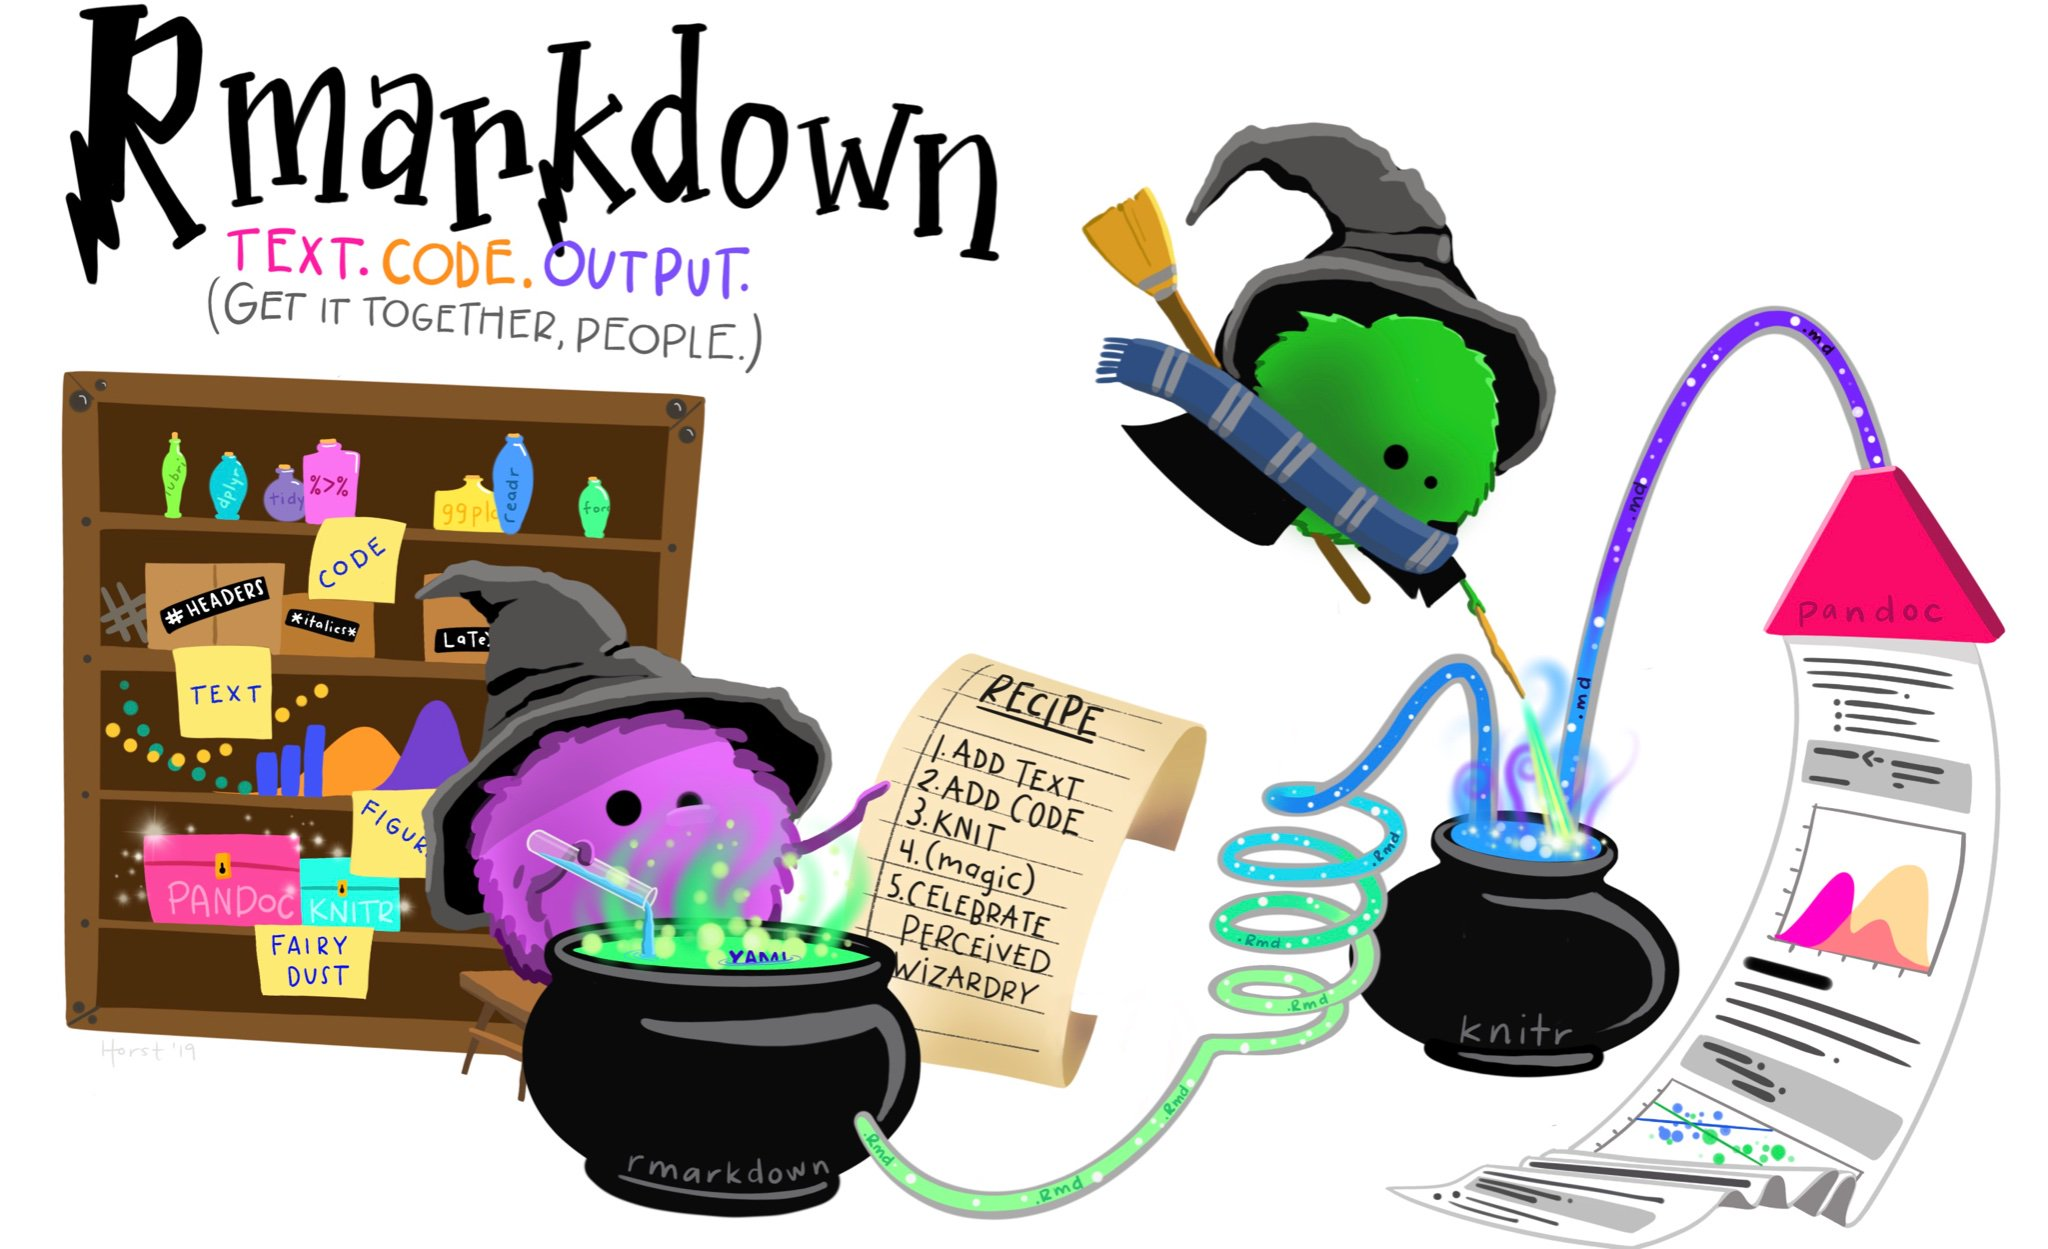
\includegraphics[width=0.8\linewidth]{images/wizard} \caption{courtesy of Allison Horst}\label{fig:unnamed-chunk-2}
\end{figure}

\hypertarget{introduction-to-r}{%
\section{Introduction to R}\label{introduction-to-r}}

\href{https://www.r-project.org/}{R} is the name of the programming language itself and \href{img/rstudio-ide.pdf}{RStudio} is a convenient interface.{]}, which we will be using throughout the course in order to learn how to organise data, produce accurate data analyses \& data visualisations.

Eventually we will also add extra tools like \href{https://www.youtube.com/watch?v=w3jLJU7DT5E}{GitHub} and \href{https://rmarkdown.rstudio.com/}{RMarkdown} for data reproducibility and collaborative programming, check out this short (and very cheesy) intro video.{]}, which are collaboration and version control systems that we will be using throughout the course. More on this in future weeks.

By the end of this module I hope you will have the tools to confidently analyze real data, make informative and beautiful data visuals, and be able to analyse lots of different types of data.

The taught content this autumn will be given to you in several \textbf{worksheets}, these will be added to this dynamic webpage each week.

\hypertarget{getting-around-on-rstudio}{%
\section{Getting around on RStudio}\label{getting-around-on-rstudio}}

All of our sessions will run on cloud-based software. All you have to do is make a free account, and join our Workspace \texttt{BIO-5023Y} the sharing link is \href{https://rstudio.cloud/spaces/84058/join?access_code=6c3uEkEUsNhbzUrttMcRq3SoSkQ4vKw\%2FeYBoyBRu}{here}.

Once you are signed up - you will see that there are two \texttt{Spaces}

\begin{itemize}
\item
  Your workspace
\item
  BIO-5023Y
\end{itemize}

Make sure you are working in the class workspace - there is a limit to the hours/month on your workspace, so all assigments and project work should take place in the \texttt{BIO-5023Y\ space}.

Watch these short explainer videos to get used to navigating the environment.

\hypertarget{an-intro-to-rstudio}{%
\subsection{An intro to RStudio}\label{an-intro-to-rstudio}}

RStudio

\begin{quote}
Note - people often mix up R and RStudio. R is the programming language (the engine), RStudio is a handy interface/wrapper that makes things a bit easier to use.
\end{quote}

\hypertarget{using-r-studio-cloud}{%
\subsection{Using R Studio Cloud}\label{using-r-studio-cloud}}

RStudio Cloud works in exactly the same way as RStudio, but means you don't have to download any software. You can access the hosted cloud server and your projects through any browser connection (Chrome works best), from any computer.

\hypertarget{reading}{%
\section{Reading}\label{reading}}

There are lots of useful books and online resources to help develop and improve your R knowledge. Throughout this webpage I will be adding useful resources for you.

The core textbook you might want to bookmark is R for Data Science \citep{R4DS} but we will add others throughout the course, and their is a bibliography at the end which collects everything together!

\hypertarget{get-help}{%
\section{Get Help!}\label{get-help}}

There are a \textbf{lot} of sources of information about using R out there.
Here are a few helpful places to get help when you have an issue, or just to learn more

\begin{itemize}
\item
  The R help system itself - we cover this in Week one \protect\hyperlink{error}{Error}
\item
  Vignettes - type \texttt{browseVignettes()} into the console and hit Enter, a list of available vignettes for all the packages we have will be displayed
\item
  \href{https://www.rstudio.com/resources/cheatsheets/}{Cheat Sheets} - available at RStudio.com. Most common packages have an associate cheat sheet covering the basics of how to use them. Download/bookmark ones we will use commonly such as \texttt{ggplot2}, \texttt{Data\ transformation\ with\ dplyr}, \texttt{Data\ tidying\ with\ tidyr} \& \texttt{Data\ import}.
\item
  Google - I use Google constantly, because I continually forget how to do even basic tasks. If I want to remind myself how to round a number, I might type something like \texttt{R\ round\ number} - if I am using a particular package I should include that in the search term as well
\item
  \href{https://web.yammer.com/main/groups/eyJfdHlwZSI6Ikdyb3VwIiwiaWQiOiI3OTAyMTk1NzEyMCJ9/all}{Ask for help} - If you are stuck, getting an error message, can't think what to do next, then ask someone. It could be me, it could be a classmate. When you do this it is very important that you \textbf{show the code}, include the \textbf{error message}. ``This doesn't work'' is not helpful. ``Here is my code, this is the data I am using, I want it to do X, and here's the problem I get''.
\end{itemize}

\begin{quote}
Note - It may be daunting to send your code to someone for help. It is natural and common to feel apprehensive, or to think that your code is really bad. I still feel the same! But we learn when we share our mistakes, and eventually you will find it funny when you look back on your early mistakes, or laugh about the mistakes you still occasionally make!
\end{quote}

\hypertarget{getting-to-know-r-week-one}{%
\chapter{Getting to know R: Week One}\label{getting-to-know-r-week-one}}

Go to RStudio Cloud and enter the Project labelled \texttt{Week\ One} - this will clone the project and provide you with your own workspace.

Follow the instructions below to get used to the R command line, and how R works as a language.

\hypertarget{your-first-r-command}{%
\section{Your first R command}\label{your-first-r-command}}

In the RStudio pane, navigate to the console (bottom left) and \texttt{type\ or\ copy} the below it should appear at the \textgreater{}

Hit Enter on your keyboard.

\begin{Shaded}
\begin{Highlighting}[]
\DecValTok{10} \SpecialCharTok{+} \DecValTok{20}
\end{Highlighting}
\end{Shaded}

You should now be looking at the below:

\begin{verbatim}
> 10 + 20
[1] 30
\end{verbatim}

The first line shows the request you made to R, the next line is R's response

You didn't type the \texttt{\textgreater{}} symbol: that's just the R command prompt and isn't part of the actual command.

It's important to understand how the output is formatted. Obviously, the correct answer to the sum \texttt{10\ +\ 20} is \texttt{30}, and not surprisingly R has printed that out as part of its response. But it's also printed out this \texttt{{[}1{]}} part, which probably doesn't make a lot of sense to you right now. You're going to see that a lot. You can think of \texttt{{[}1{]}\ 30} as if R were saying ``the answer to the 1st question you asked is 30''.

\hypertarget{typos}{%
\subsection{Typos}\label{typos}}

Before we go on to talk about other types of calculations that we can do with R, there's a few other things I want to point out. The first thing is that, while R is good software, it's still software. It's pretty stupid, and because it's stupid it can't handle typos. It takes it on faith that you meant to type \emph{exactly} what you did type. For example, suppose that you forgot to hit the shift key when trying to type \texttt{+}, and as a result your command ended up being \texttt{10\ =\ 20} rather than \texttt{10\ +\ 20}. Try it for yourself and replicate this error message:

\begin{Shaded}
\begin{Highlighting}[]
\DecValTok{10} \OtherTok{=} \DecValTok{20}
\end{Highlighting}
\end{Shaded}

\begin{verbatim}
## Error in 10 = 20: invalid (do_set) left-hand side to assignment
\end{verbatim}

What's happened here is that R has attempted to interpret \texttt{10\ =\ 20} as a command, and spits out an error message because the command doesn't make any sense to it. When a \emph{human} looks at this, and then looks down at his or her keyboard and sees that \texttt{+} and \texttt{=} are on the same key, it's pretty obvious that the command was a typo. But R doesn't know this, so it gets upset. And, if you look at it from its perspective, this makes sense. All that R ``knows'' is that \texttt{10} is a legitimate number, \texttt{20} is a legitimate number, and \texttt{=} is a legitimate part of the language too. In other words, from its perspective this really does look like the user meant to type \texttt{10\ =\ 20}, since all the individual parts of that statement are legitimate and it's too stupid to realise that this is probably a typo. Therefore, R takes it on faith that this is exactly what you meant\ldots{} it only ``discovers'' that the command is nonsense when it tries to follow your instructions, typo and all. And then it whinges, and spits out an error.

Even more subtle is the fact that some typos won't produce errors at all, because they happen to correspond to ``well-formed'' R commands. For instance, suppose that not only did I forget to hit the shift key when trying to type \texttt{10\ +\ 20}, I also managed to press the key next to one I meant do. The resulting typo would produce the command \texttt{10\ -\ 20}. Clearly, R has no way of knowing that you meant to \emph{add} 20 to 10, not \emph{subtract} 20 from 10, so what happens this time is this:

\begin{Shaded}
\begin{Highlighting}[]
\DecValTok{10} \SpecialCharTok{{-}} \DecValTok{20}
\end{Highlighting}
\end{Shaded}

\begin{verbatim}
## [1] -10
\end{verbatim}

In this case, R produces the right answer, but to the the wrong question.

\hypertarget{more-simple-arithmetic}{%
\subsection{More simple arithmetic}\label{more-simple-arithmetic}}

One of the best ways to get to know R is to play with it, it's pretty difficult to break it so don't worry too much. Type whatever you want into to the console and see what happens.

If the last line of your console looks like this

\begin{verbatim}
> 10+
+ 
\end{verbatim}

and there's a blinking cursor next to the plus sign. This means is that R is still waiting for you to finish. It ``thinks'' you're still typing your command, so it hasn't tried to execute it yet. In other words, this plus sign is actually another command prompt. It's different from the usual one (i.e., the \texttt{\textgreater{}} symbol) to remind you that R is going to ``add'' whatever you type now to what you typed last time. For example, type \texttt{20} and hit enter, then it finishes the command:

\begin{verbatim}
> 10 +
+ 20
[1] 30
\end{verbatim}

\emph{Alternatively} hit escape, and R will forget what you were trying to do and return to a blank line.

\hypertarget{try-some-maths}{%
\subsection{Try some maths}\label{try-some-maths}}

\begin{Shaded}
\begin{Highlighting}[]
\DecValTok{1}\SpecialCharTok{+}\DecValTok{7}
\end{Highlighting}
\end{Shaded}

\begin{Shaded}
\begin{Highlighting}[]
\DecValTok{13{-}10}
\end{Highlighting}
\end{Shaded}

\begin{Shaded}
\begin{Highlighting}[]
\DecValTok{4}\SpecialCharTok{*}\DecValTok{6}
\end{Highlighting}
\end{Shaded}

\begin{Shaded}
\begin{Highlighting}[]
\DecValTok{12}\SpecialCharTok{/}\DecValTok{3}
\end{Highlighting}
\end{Shaded}

Raise a number to the power of another

\begin{Shaded}
\begin{Highlighting}[]
\DecValTok{5}\SpecialCharTok{\^{}}\DecValTok{4}
\end{Highlighting}
\end{Shaded}

As I'm sure everyone will probably remember the moment they read this, the act of multiplying a number \(x\) by itself \(n\) times is called ``raising \(x\) to the \(n\)-th power''. Mathematically, this is written as \(x^n\). Some values of \(n\) have special names: in particular \(x^2\) is called \(x\)-squared, and \(x^3\) is called \(x\)-cubed. So, the 4th power of 5 is calculated like this:
\[
5^4 = 5 \times 5 \times 5 \times 5 
\]

\hypertarget{perform-some-combos}{%
\subsection{Perform some combos}\label{perform-some-combos}}

Perform some mathematical combos, noting that the order in which R performs calculations is the standard one.

That is, first calculate things inside \textbf{B}rackets \texttt{()}, then calculate \textbf{O}rders of (exponents) \texttt{\^{}}, then \textbf{D}ivision \texttt{/} and \textbf{M}ultiplication \texttt{*}, then \textbf{A}ddition \texttt{+} and \textbf{S}ubtraction \texttt{-}.

Notice the different outputs of these two commands.

\begin{Shaded}
\begin{Highlighting}[]
\DecValTok{3}\SpecialCharTok{\^{}}\DecValTok{2{-}5}\SpecialCharTok{/}\DecValTok{2}
\end{Highlighting}
\end{Shaded}

\begin{Shaded}
\begin{Highlighting}[]
\NormalTok{(}\DecValTok{3}\SpecialCharTok{\^{}}\DecValTok{2{-}5}\NormalTok{)}\SpecialCharTok{/}\DecValTok{2}
\end{Highlighting}
\end{Shaded}

Similarly if we want to raise a number to a fraction, we need to surround the fraction with parentheses ()

\begin{Shaded}
\begin{Highlighting}[]
\DecValTok{16}\SpecialCharTok{\^{}}\DecValTok{1}\SpecialCharTok{/}\DecValTok{2}
\end{Highlighting}
\end{Shaded}

\begin{Shaded}
\begin{Highlighting}[]
\DecValTok{16}\SpecialCharTok{\^{}}\NormalTok{(}\DecValTok{1}\SpecialCharTok{/}\DecValTok{2}\NormalTok{)}
\end{Highlighting}
\end{Shaded}

The first one calculates 16 raised to the power of 1, then divided this answer by two. The second one raises 16 to the power of a half. A big difference in the output.

\begin{quote}
**Note - While the cursor is in the console, you can press the up arrow to see all your previous commands.
You can run them again, or edit them. Later on we will look at scripts, as an essential way to re-use, store and edit commands.
\end{quote}

\hypertarget{true-or-false-data}{%
\section{``true or false'' data}\label{true-or-false-data}}

Time to make a sidebar onto another kind of data. A key concept in that a lot of R relies on is the idea of a \textbf{\emph{logical value}}. A logical value is an assertion about whether something is true or false. This is implemented in R in a pretty straightforward way. There are two logical values, namely \texttt{TRUE} and \texttt{FALSE}. Despite the simplicity, a logical values are very useful things. Let's see how they work.

\hypertarget{assessing-mathematical-truths}{%
\subsection{Assessing mathematical truths}\label{assessing-mathematical-truths}}

In George Orwell's classic book \emph{1984}, one of the slogans used by the totalitarian Party was ``two plus two equals five'', the idea being that the political domination of human freedom becomes complete when it is possible to subvert even the most basic of truths.

But they didn't have R. R will not be subverted. It has rather firm opinions on the topic of what is and isn't true, at least as regards basic mathematics. If I ask it to calculate \texttt{2\ +\ 2}, it always gives the same answer, and it's not bloody 5:

\begin{Shaded}
\begin{Highlighting}[]
\DecValTok{2} \SpecialCharTok{+} \DecValTok{2}
\end{Highlighting}
\end{Shaded}

Of course, so far R is just doing the calculations. I haven't asked it to explicitly assert that \(2+2 = 4\) is a true statement. If I want R to make an explicit judgement, I can use a command like this:

\begin{Shaded}
\begin{Highlighting}[]
\DecValTok{2} \SpecialCharTok{+} \DecValTok{2} \SpecialCharTok{==} \DecValTok{4}
\end{Highlighting}
\end{Shaded}

What I've done here is use the \textbf{\emph{equality operator}}, \texttt{==}, to force R to make a ``true or false'' judgement.

\begin{quote}
**Note that this is a very different operator to the assignment operator \texttt{=} you saw previously. A common typo that people make when trying to write logical commands in R (or other languages, since the ``\texttt{=} versus \texttt{==}'' distinction is important in most programming languages) is to accidentally type \texttt{=} when you really mean \texttt{==}.
\end{quote}

Okay, let's see what R thinks of the Party slogan:

\begin{Shaded}
\begin{Highlighting}[]
\DecValTok{2}\SpecialCharTok{+}\DecValTok{2} \SpecialCharTok{==} \DecValTok{5}
\end{Highlighting}
\end{Shaded}

Take that Big Brother! Anyway, it's worth having a look at what happens if I try to \emph{force} R to believe that two plus two is five by making an assignment statement like \texttt{2\ +\ 2\ =\ 5} or \texttt{2\ +\ 2\ \textless{}-\ 5}. When I do this, here's what happens:

\begin{Shaded}
\begin{Highlighting}[]
\DecValTok{2} \SpecialCharTok{+} \DecValTok{2} \OtherTok{=} \DecValTok{5}
\end{Highlighting}
\end{Shaded}

R doesn't like this very much. It recognises that \texttt{2\ +\ 2} is \emph{not} a variable (that's what the ``non-language object'' part is saying), and it won't let you try to ``reassign'' it. While R is pretty flexible, and actually does let you do some quite remarkable things to redefine parts of R itself, there are just some basic, primitive truths that it refuses to give up. It won't change the laws of addition, and it won't change the definition of the number \texttt{2}.

That's probably for the best.

\hypertarget{storing-outputs}{%
\section{Storing outputs}\label{storing-outputs}}

With simple questions like the ones above we are happy to just see the answer, but our quesitons are often more complex than this. If we need to take multiple steps, we benefit from being able to store our answers and recall them for use in later steps. This is very simple to do we can \emph{assign} outputs to a name:

\begin{Shaded}
\begin{Highlighting}[]
\NormalTok{a }\OtherTok{\textless{}{-}} \DecValTok{1}\SpecialCharTok{+}\DecValTok{2}
\end{Highlighting}
\end{Shaded}

This literally means please \emph{assign} the value of \texttt{1+2} to the name \texttt{a}. We use the \textbf{assignment operator} \texttt{\textless{}-} to make this assignment.

\begin{quote}
**Note the shortcut key for \textless- is Alt + - (Windows) or Option + - (Mac)
\end{quote}

If you perform this action you should be able to do two things

\begin{itemize}
\item
  You should be able to see that in the top right-hand pane in the \texttt{Environment} tab their is now an \texttt{object} called a with the value of 3.
\item
  You should be able to look at what a is by typing it into your Console and pressing Enter
\end{itemize}

\begin{Shaded}
\begin{Highlighting}[]
\NormalTok{a}
\end{Highlighting}
\end{Shaded}

\begin{verbatim}
> a
[1] 3
\end{verbatim}

You can now call this object at any time during your R session and perform calculations with it.

\begin{Shaded}
\begin{Highlighting}[]
\DecValTok{2} \SpecialCharTok{*}\NormalTok{ a}
\end{Highlighting}
\end{Shaded}

\begin{verbatim}
[1] 6
\end{verbatim}

What happens if we assign a value to a named object that already exists in our R environment??? for example

\begin{Shaded}
\begin{Highlighting}[]
\NormalTok{a }\OtherTok{\textless{}{-}} \DecValTok{10}
\NormalTok{a}
\end{Highlighting}
\end{Shaded}

\begin{verbatim}
[1] 10
\end{verbatim}

You should see that the previous assignment is lost, \emph{gone forever} and has been replaced by the new value.

We can assign lots of things to objects, and use them in calculations to build more objects.

\begin{Shaded}
\begin{Highlighting}[]
\NormalTok{b }\OtherTok{\textless{}{-}} \DecValTok{5}
\NormalTok{c }\OtherTok{\textless{}{-}}\NormalTok{ a }\SpecialCharTok{+}\NormalTok{ b}
\end{Highlighting}
\end{Shaded}

Note that if you now change the value of b, the value of c does \emph{not} change. Objects are totally independent from each other once they are made

\begin{Shaded}
\begin{Highlighting}[]
\NormalTok{b }\OtherTok{\textless{}{-}} \DecValTok{7}
\NormalTok{b}
\NormalTok{c}
\end{Highlighting}
\end{Shaded}

Look at the environment tab again - you should see it's starting to fill up now!

\begin{quote}
**Note - RStudio will by default save the objects in its memory when you close a session. These will then be there the next time you logon. It might seem nice to be able to close things down and pick up where you left off, but its actually quite dangerous. It's messy, and can cause lots of problems when we work with scripts later, so don't do this!!! To stop RStudio from saving objects by default go to the Preferences option and change ``Save workspace to .RData on exit'' to ``Never''. Instead we are going to learn how to use scripts to quickly re-run analyses we have been working on.
\end{quote}

\hypertarget{choosing-names}{%
\subsection{Choosing names}\label{choosing-names}}

\begin{itemize}
\item
  Use informative variable names. As a general rule, using meaningful names like \texttt{orange} and \texttt{apple} is preferred over arbitrary ones like \texttt{variable1} and \texttt{variable2}. Otherwise it's very hard to remember what the contents of different variables actually are.
\item
  Use short variable names. Typing is a pain and no-one likes doing it. So we much prefer to use a name like \texttt{apple} over a name like \texttt{pink\_lady\_apple}.
\item
  Use one of the conventional naming styles for multi-word variable names. R only lets you use certain things as \textbf{legal} names. Legal names must start with a letter \textbf{not} a number, which can then be followed by a sequence of letters, numbers, ., or \_. R does not like using spaces. Upper and lower case names are allowed, but R is case sensitive so \texttt{Apple} and \texttt{apple} are different.
\item
  My favourite naming convention is \texttt{snake\_case} short, lower case only, spaces between words are separated with a \_. It's easy to read and easy to remember.
\end{itemize}

\hypertarget{writing-scripts}{%
\section{Writing scripts}\label{writing-scripts}}

Until now we have been typing words directly into the Console. This is fine for short/simple calculations - but as soon as we have a more complex, multi-step process this becomes time consuming, error-prone and \emph{boring}. \textbf{Scripts} are a document containing all of your commands (in the order you want them to run), they are \emph{repeatable, shareable, annotated records of what you have done}. In short they are incredibly useful - and a big step towards \textbf{open} and \textbf{reproducible} research.

To create a script go to File \textgreater{} New File \textgreater{} R Script.

This will open a pane in the top-left of RStudio with a tab name of \texttt{Untitled1}. In your new script, type some of the basic arithmetic and assignment commands you used previously. When you write a script, make sure it has all of the commands you need to complete your analysis, \emph{in the order you want them to run}.

\hypertarget{commenting-on-scripts}{%
\subsection{Commenting on scripts}\label{commenting-on-scripts}}

Annotating your instructions provides yourself and others insights into why you are doing what you are doing. This is a vital aspect of a robust and reproducible workflow. And when you come back to a script, one week, one month or one year from now you will often wonder what a command was for. It is very, very useful to make notes for yourself, and its useful in case anyone else will ever read your script. Make these comments helpful they are for humans to read.

In R we signal a comment with the \# key. Everything in the line after a \# is ignored by R and won't be treated as a command. You should see that it is marked in a different colour in your script.

Put the following comment in your script. Try adding a few comments to your previous lines of code

\begin{Shaded}
\begin{Highlighting}[]
\CommentTok{\# I really love R}
\end{Highlighting}
\end{Shaded}

\hypertarget{running-your-script}{%
\subsection{Running your script}\label{running-your-script}}

To run the commands from your script, we need to get it into the Console. You could select and copy/paste this into the Console. But there are a couple of faster shortcuts.

\begin{itemize}
\item
  Hit the Run button in the top right of the script pane. Pressing this will run the line of code the cursor is sitting on.
\item
  Pressing Ctrl+Enter will do the same thing as hitting the Run button
\item
  If you want to run the whole script in one go then press Ctrl+A then either click Run or press Ctrl+Enter
\end{itemize}

\hypertarget{saving-your-script}{%
\subsection{Saving your script}\label{saving-your-script}}

Our script now contains code and comments from our first workshop. We need to save it.

Alongside our data, our script is the most precious part of our analysis. We don't need to save anything else, any outputs etc. because our script can always be used to generate everything again. Note the colour of the script - the name changes colour when we have unsaved changes. Press the Save button or go to File \textgreater{} Save as.
Give the File a sensible name like ``Simple commands in R'' and in the bottom right pane under \texttt{Files} you should now be able to see your saved script.

You could now safely quit R, and when you log on next time to this project, your script will be waiting for you.

\hypertarget{error}{%
\section{Error}\label{error}}

Things will go wrong eventually, they always do\ldots{}

R is \emph{very} pedantic, even the smallest typo can result in failure and typos are impossilbe to avoid. So we will make mistakes. One type of mistake we will make is an \textbf{error}. The code fails to run. The most common causes for an error are:

\begin{itemize}
\item
  typos
\item
  missing commas
\item
  missing brackets
\end{itemize}

There's nothing wrong with making \emph{lots} of errors. The trick is not to panic or get frustrated, but to read the error message and our script carefully and start to \emph{debug}\ldots{}

\ldots{} and sometimes we need to walk away and come back later!

\begin{figure}

\includegraphics[width=0.8\linewidth]{images/Error} \caption{courtesy of Allison Horst}\label{fig:unnamed-chunk-28}
\end{figure}

\hypertarget{functions}{%
\section{Functions}\label{functions}}

Functions are the tools of R. Each one helps us to do a different task.

Take for example the function that we use to round a number to a certain number of digits - this function is called \texttt{round}

Here's an example

\begin{Shaded}
\begin{Highlighting}[]
\FunctionTok{round}\NormalTok{(}\AttributeTok{x  =} \FloatTok{2.4326782647}\NormalTok{, }\AttributeTok{digits =} \DecValTok{2}\NormalTok{)}
\end{Highlighting}
\end{Shaded}

We start the command with the function name \texttt{round}. The name is followed by parentheses (). Within these we place the \emph{arguments} for the function, each of which is separated by a comma.

The arguments

\begin{itemize}
\item
  x = 2.4326782647
\item
  digits = 2
\end{itemize}

Arguments are the information we give to a function. These arguments are in the form \texttt{name\ =\ value} the name specifies the argument, and the value is what we are providing. That is the first argument x is the number we would like to round, it has a value of 2.4326782647. The second argument digits is how we would like the number to be rounded and we specify 2.

Ok put the above commmand in your script and add a comment with \# as to what you are doing.

\hypertarget{storing-the-output-of-functions}{%
\subsection{Storing the output of functions}\label{storing-the-output-of-functions}}

What if we need the answer from a function in a later calculation. The answer is to use the assignment operator again.

Can you work out what is going on here? If so copy this into your R script and a \#comment next to each line.

\begin{Shaded}
\begin{Highlighting}[]
\NormalTok{number\_of\_digits }\OtherTok{\textless{}{-}} \DecValTok{2}
\NormalTok{my\_number }\OtherTok{\textless{}{-}} \FloatTok{2.4326782647}
\NormalTok{rounded\_number }\OtherTok{\textless{}{-}} \FunctionTok{round}\NormalTok{(}\AttributeTok{x  =}\NormalTok{ my\_number, }
                        \AttributeTok{digits =}\NormalTok{ number\_of\_digits)}
\end{Highlighting}
\end{Shaded}

\hypertarget{more-fun-with-functions}{%
\subsection{More fun with functions}\label{more-fun-with-functions}}

Check this out

\begin{Shaded}
\begin{Highlighting}[]
\FunctionTok{round}\NormalTok{(}\FloatTok{2.4326782647}\NormalTok{, }\DecValTok{2}\NormalTok{)}
\end{Highlighting}
\end{Shaded}

We don't \emph{have} to give the names of arguments for a function to still work. This works because the function \texttt{round} expects us to give the number value first, and the argument for rounding digits second. \emph{But} this assumes we know the expected ordering within a function, this might be the case for functions we use a lot. If you give arguments their proper names \emph{then} you can actually introduce them in any order you want.

Try this:

\begin{Shaded}
\begin{Highlighting}[]
\FunctionTok{round}\NormalTok{(}\AttributeTok{digits =} \DecValTok{2}\NormalTok{, }\AttributeTok{x  =} \FloatTok{2.4326782647}\NormalTok{)}
\end{Highlighting}
\end{Shaded}

But this gives a different answer

\begin{Shaded}
\begin{Highlighting}[]
\FunctionTok{round}\NormalTok{(}\DecValTok{2}\NormalTok{, }\FloatTok{2.4326782647}\NormalTok{)}
\end{Highlighting}
\end{Shaded}

Are you happy with what is happening here? naming arguments overrides the position defaults

Ok what about this?

\begin{Shaded}
\begin{Highlighting}[]
\FunctionTok{round}\NormalTok{(}\FloatTok{2.4326782647}\NormalTok{)}
\end{Highlighting}
\end{Shaded}

We didn't specify how many digits to round to, but we still got an answer. That's because in many functions arguments have \texttt{defaults} - the default argument here is digits = 0. So we don't have to specify the argument if we are happy for round to produce whole numbers.

How do we know argument orders and defaults? Well we get to know how a lot of functions work through practice, but we can also use the inbuilt R help. This is a function - but now we specify the name of another function to provide a help menu.

\begin{Shaded}
\begin{Highlighting}[]
\FunctionTok{help}\NormalTok{(round)}
\end{Highlighting}
\end{Shaded}

\hypertarget{packages}{%
\section{Packages}\label{packages}}

An R package is a container for various things including functions and data. These make it easy to do very complicate protocols by using custom-built functions. Later we will see how we can write our own simple functions.

On RStudio Cloud I have already installed several add-on packages, all we need to do is use a simple function to load these packages into our workspace. Once this is complete we will have access to all the custom functions they contain.

Let's try that now:

\begin{Shaded}
\begin{Highlighting}[]
\FunctionTok{library}\NormalTok{(ggplot2)}
\FunctionTok{library}\NormalTok{(palmerpenguins)}
\end{Highlighting}
\end{Shaded}

\begin{quote}
Errors part 2 Another common source of errors is to call a function that is part of a package but forgetting to load the package. If R says something like ``Error in function-name'' then most likely the function was misspelled or the package containing the function hasn't been loaded.
\end{quote}

Packages are a lot like new apps extending the functionality of what your phone can do. To use the functionalities of a package they must be loaded \emph{before} we call on the funcitons or data they contain. So the most sensible place to put library calls for packages is at the very \textbf{top} of our script. So let's do that now.

\hypertarget{my-first-data-visualisation}{%
\section{My first data visualisation}\label{my-first-data-visualisation}}

Let's run our first data visualisation using the functions and data we have now loaded - this produces a plot using functions from the \texttt{ggplot2} package (\citet{R-ggplot2}) and data from the \texttt{palmerpenguins} (\citet{R-palmerpenguins}) package. Use the \# comments to add notes on what you are using each package for in your script.

Using these functions we can write a simple line of code to produce a figure. We specify the data source, the variables to be used for the x and y axis and then the type of visual object to produce, colouring them by the species.

Copy this into your console and hit Enter.

\begin{Shaded}
\begin{Highlighting}[]
\FunctionTok{ggplot}\NormalTok{(}\AttributeTok{data =}\NormalTok{ penguins,}\FunctionTok{aes}\NormalTok{(}\AttributeTok{x =}\NormalTok{ bill\_length\_mm, }\AttributeTok{y =}\NormalTok{ bill\_depth\_mm)) }\SpecialCharTok{+} \FunctionTok{geom\_point}\NormalTok{(}\FunctionTok{aes}\NormalTok{(}\AttributeTok{colour=}\NormalTok{species)) }
\end{Highlighting}
\end{Shaded}

\begin{quote}
**Note - you may have noticed R gave you a warning. Not the same as a big scary error, but R wants you to be aware of something. In this case that two of the observations had missing data in them (either bill length or bill depth), so couldn't be plotted.
\end{quote}

The above command can also be written as below, its in a longer style with each new line for each argument in the function. This style can be easier to read, and makes it easier to write comments with \#. Copy this longer command into your \texttt{script} then run it by either highlighting the entire command or placing the cursor in the first line and then hit Run or Ctrl+Enter.

\begin{Shaded}
\begin{Highlighting}[]
\FunctionTok{ggplot}\NormalTok{(}\AttributeTok{data =}\NormalTok{ penguins, }\CommentTok{\# calls ggplot function, data is penguins}
       \FunctionTok{aes}\NormalTok{(}\AttributeTok{x =}\NormalTok{ bill\_length\_mm, }\CommentTok{\# sets x axis as bill length}
           \AttributeTok{y =}\NormalTok{ bill\_depth\_mm)) }\SpecialCharTok{+} \CommentTok{\# sets y axis value as bill depth}
    \FunctionTok{geom\_point}\NormalTok{(}\FunctionTok{aes}\NormalTok{(}\AttributeTok{colour=}\NormalTok{species)) }\CommentTok{\# plot points coloured by penguin species}
\end{Highlighting}
\end{Shaded}

\hypertarget{quitting}{%
\section{Quitting}\label{quitting}}

\begin{itemize}
\item
  Make sure you have saved any changes to your R script - that's all you need to make sure you've done!
\item
  If you want me to take a look at your script let me know
\item
  If you spotted any mistakes or errors let me know
\item
  Close your RStudio Cloud Browser
\item
  Go to Blackboard to complete a short quiz!
\end{itemize}

\hypertarget{workflow-part-one-week-two}{%
\chapter{Workflow Part One: Week Two}\label{workflow-part-one-week-two}}

Last week we got acquainted with some of the core skills associated with using R and RStudio.

In this workshop we work through the journey of importing and tidying data. Once we have a curated and cleaned dataset we can work on generating insights from the data.

We are going to be working as though we are in the latter stages of a research project, where data has been collected, possibly over several years, to test against our hypotheses.

We have chosen to continue working with a dataset you have been introduced to already - the Palmer Penguins dataset. Previously we loaded a cleaned dataset, very quickly using an R package. Today we will be working in a more realistic scenario - uploading out dataset to our R workspace.

\hypertarget{meet-the-penguins}{%
\section{Meet the Penguins}\label{meet-the-penguins}}

This data, taken from the \texttt{palmerpenguins} (\citet{R-palmerpenguins}) package was originally published by \citet{Antarctic}.

The palmerpenguins data contains size measurements, clutch observations, and blood isotope ratios for three penguin species observed on three islands in the Palmer Archipelago, Antarctica over a study period of three years.

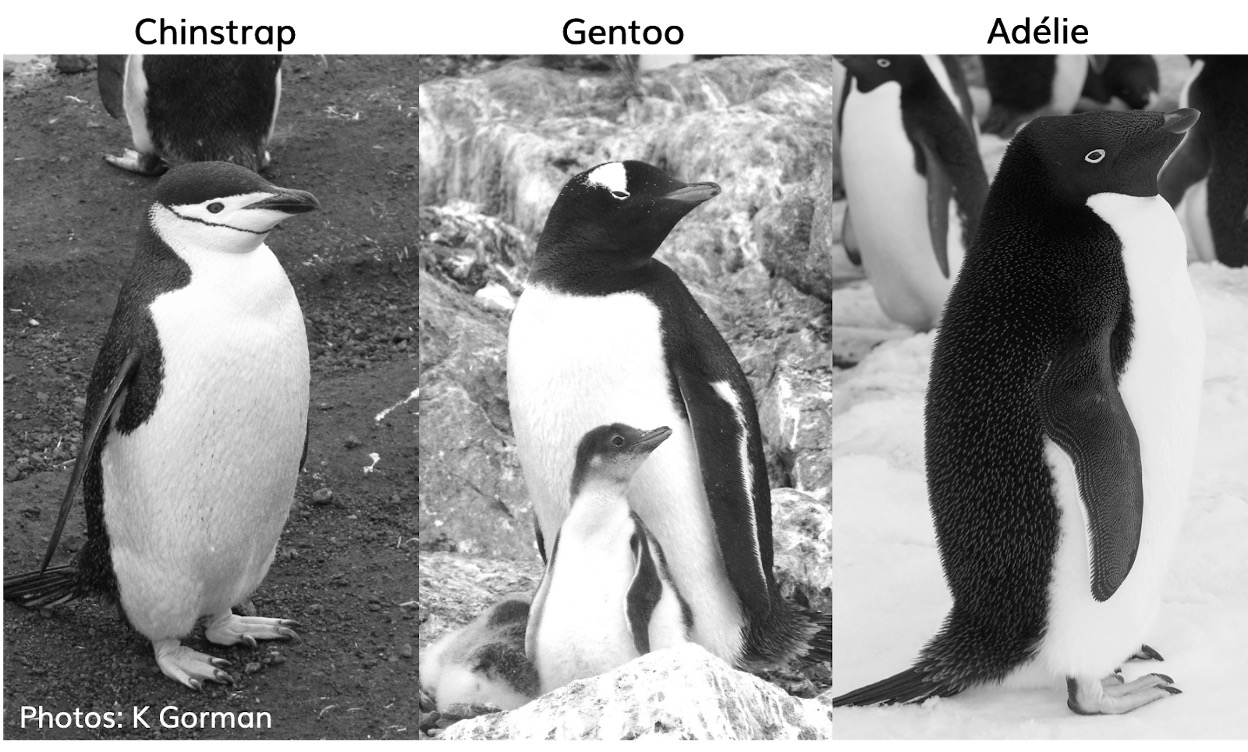
\includegraphics[width=0.8\linewidth]{images/gorman-penguins}

These data were collected from 2007 - 2009 by Dr.~Kristen Gorman with the Palmer Station Long Term Ecological Research Program, part of the US Long Term Ecological Research Network. The data were imported directly from the Environmental Data Initiative (EDI) Data Portal, and are available for use by CC0 license (``No Rights Reserved'') in accordance with the Palmer Station Data Policy. We gratefully acknowledge Palmer Station LTER and the US LTER Network. Special thanks to Marty Downs (Director, LTER Network Office) for help regarding the data license \& use. Here is our intrepid package co-author, Dr.~Gorman, in action collecting some penguin data:

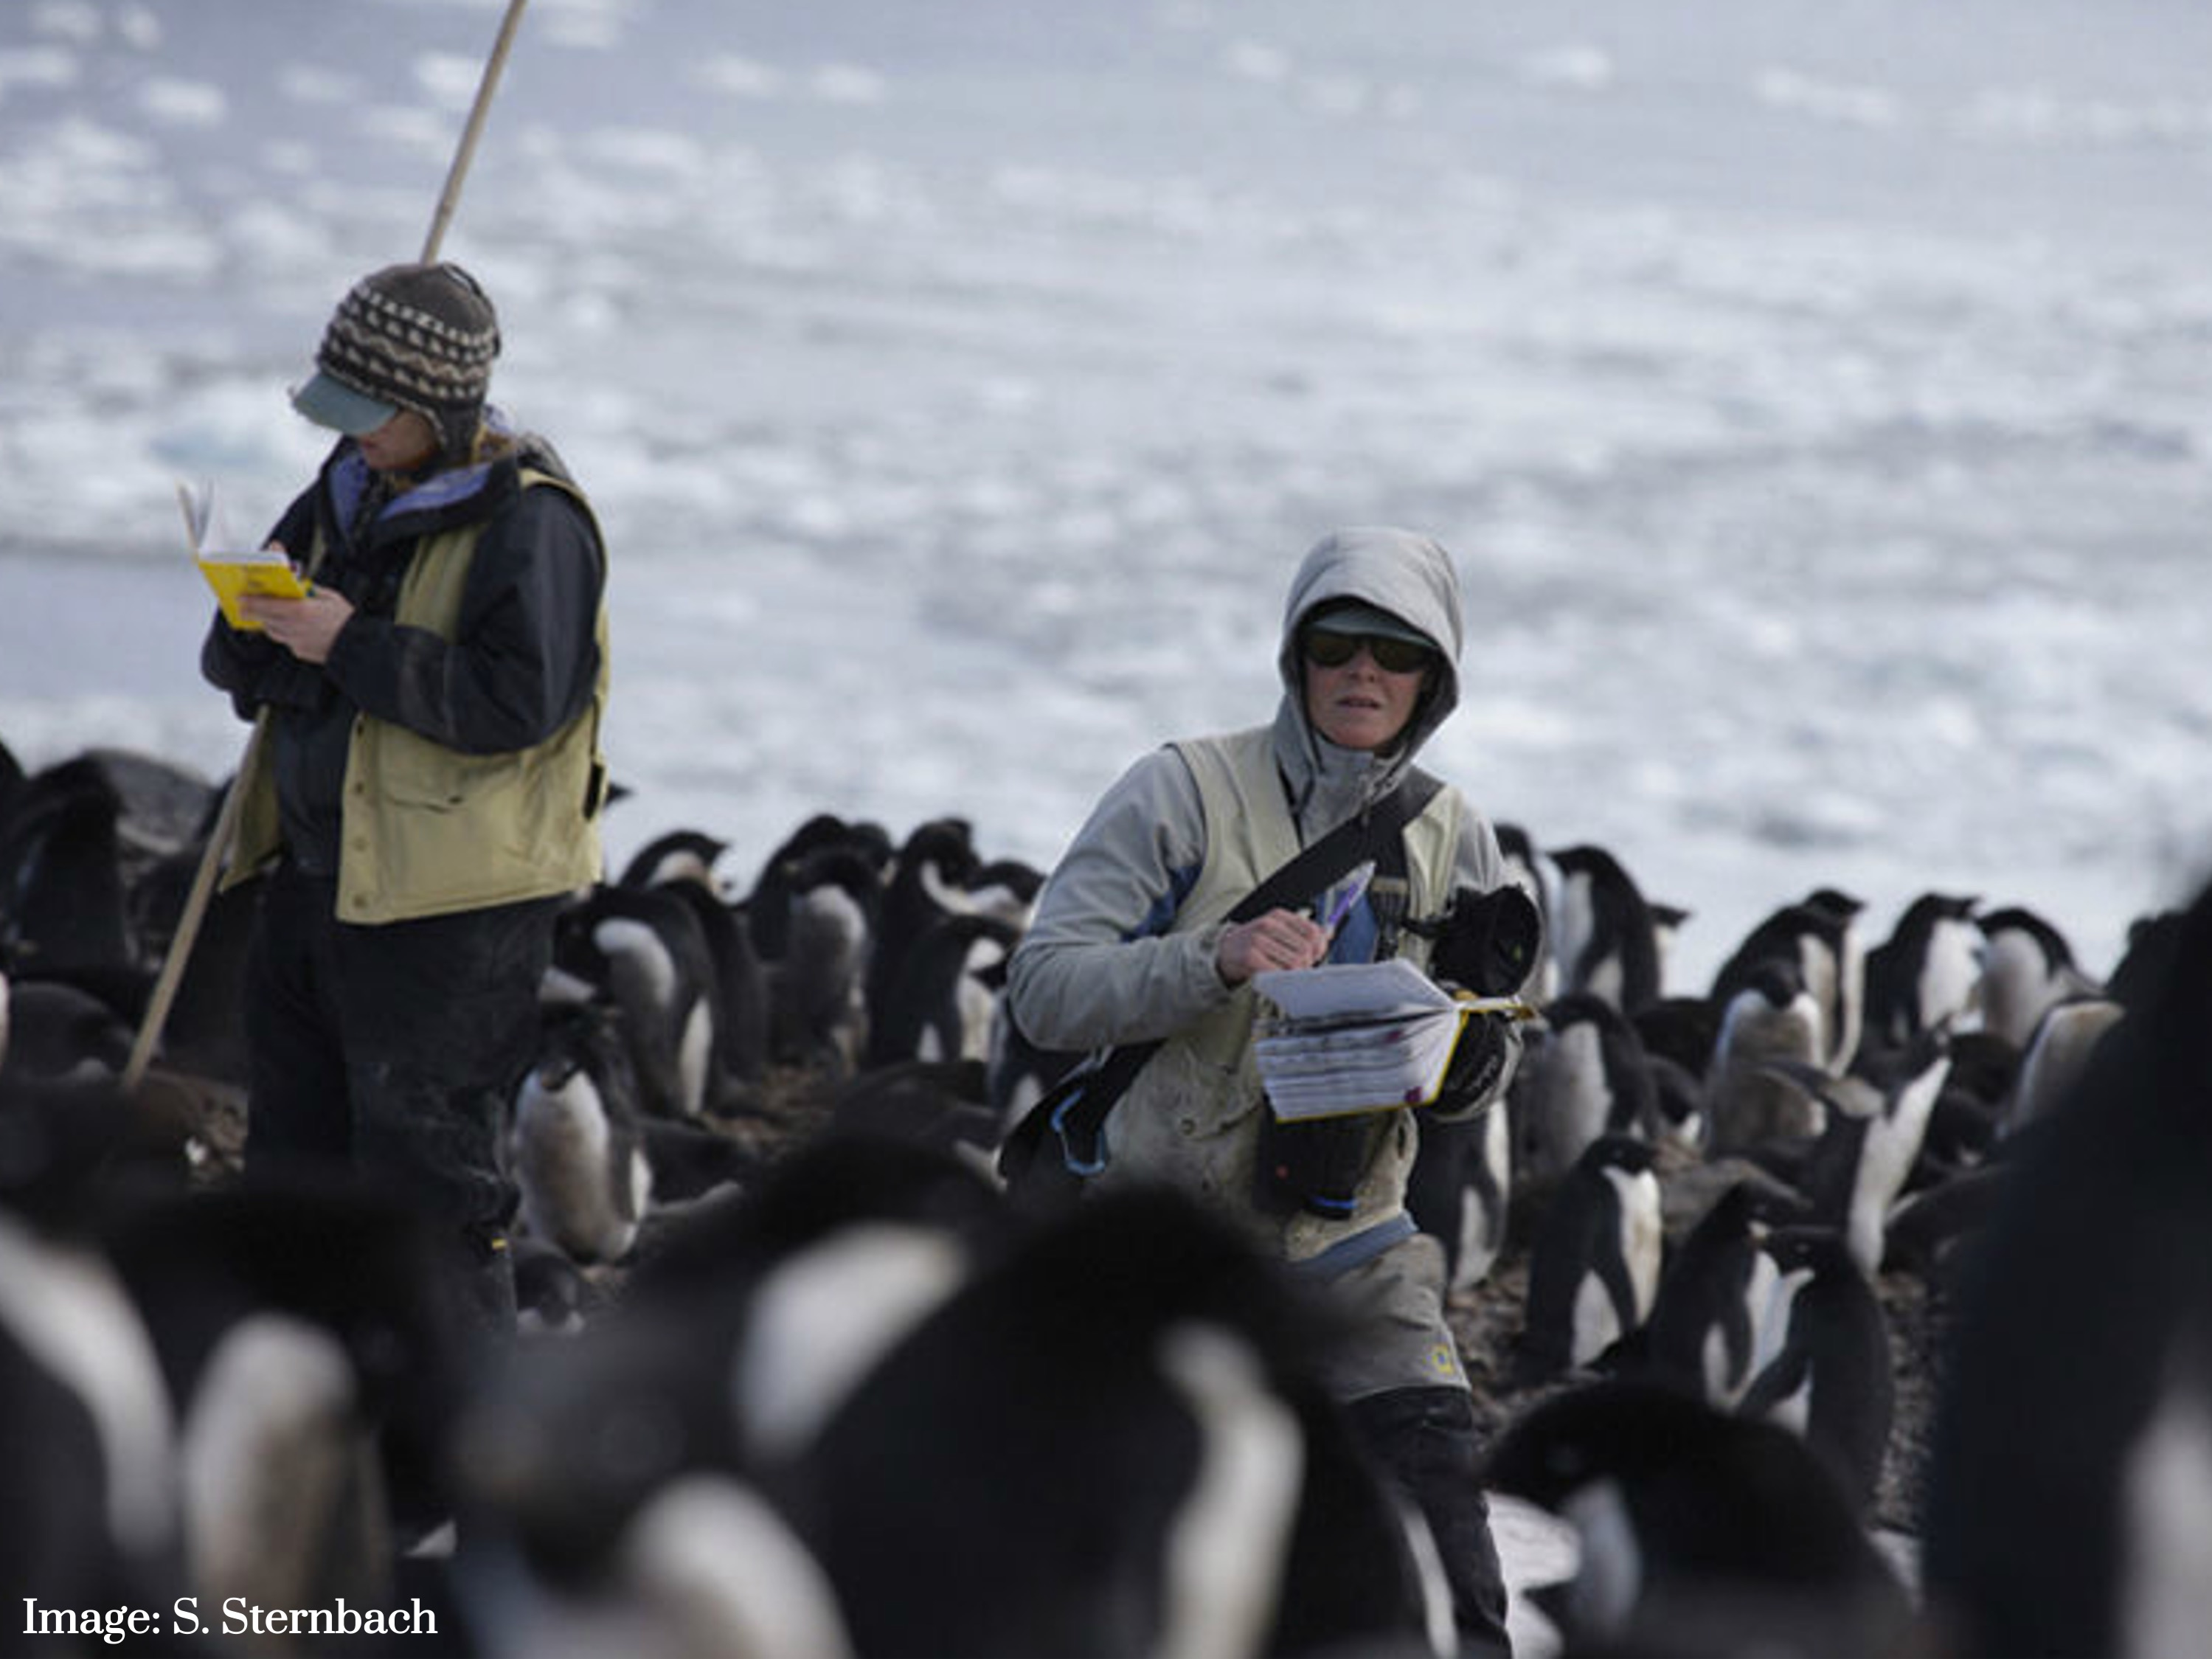
\includegraphics[width=0.8\linewidth]{images/penguin-expedition}

Here is a map of the study site

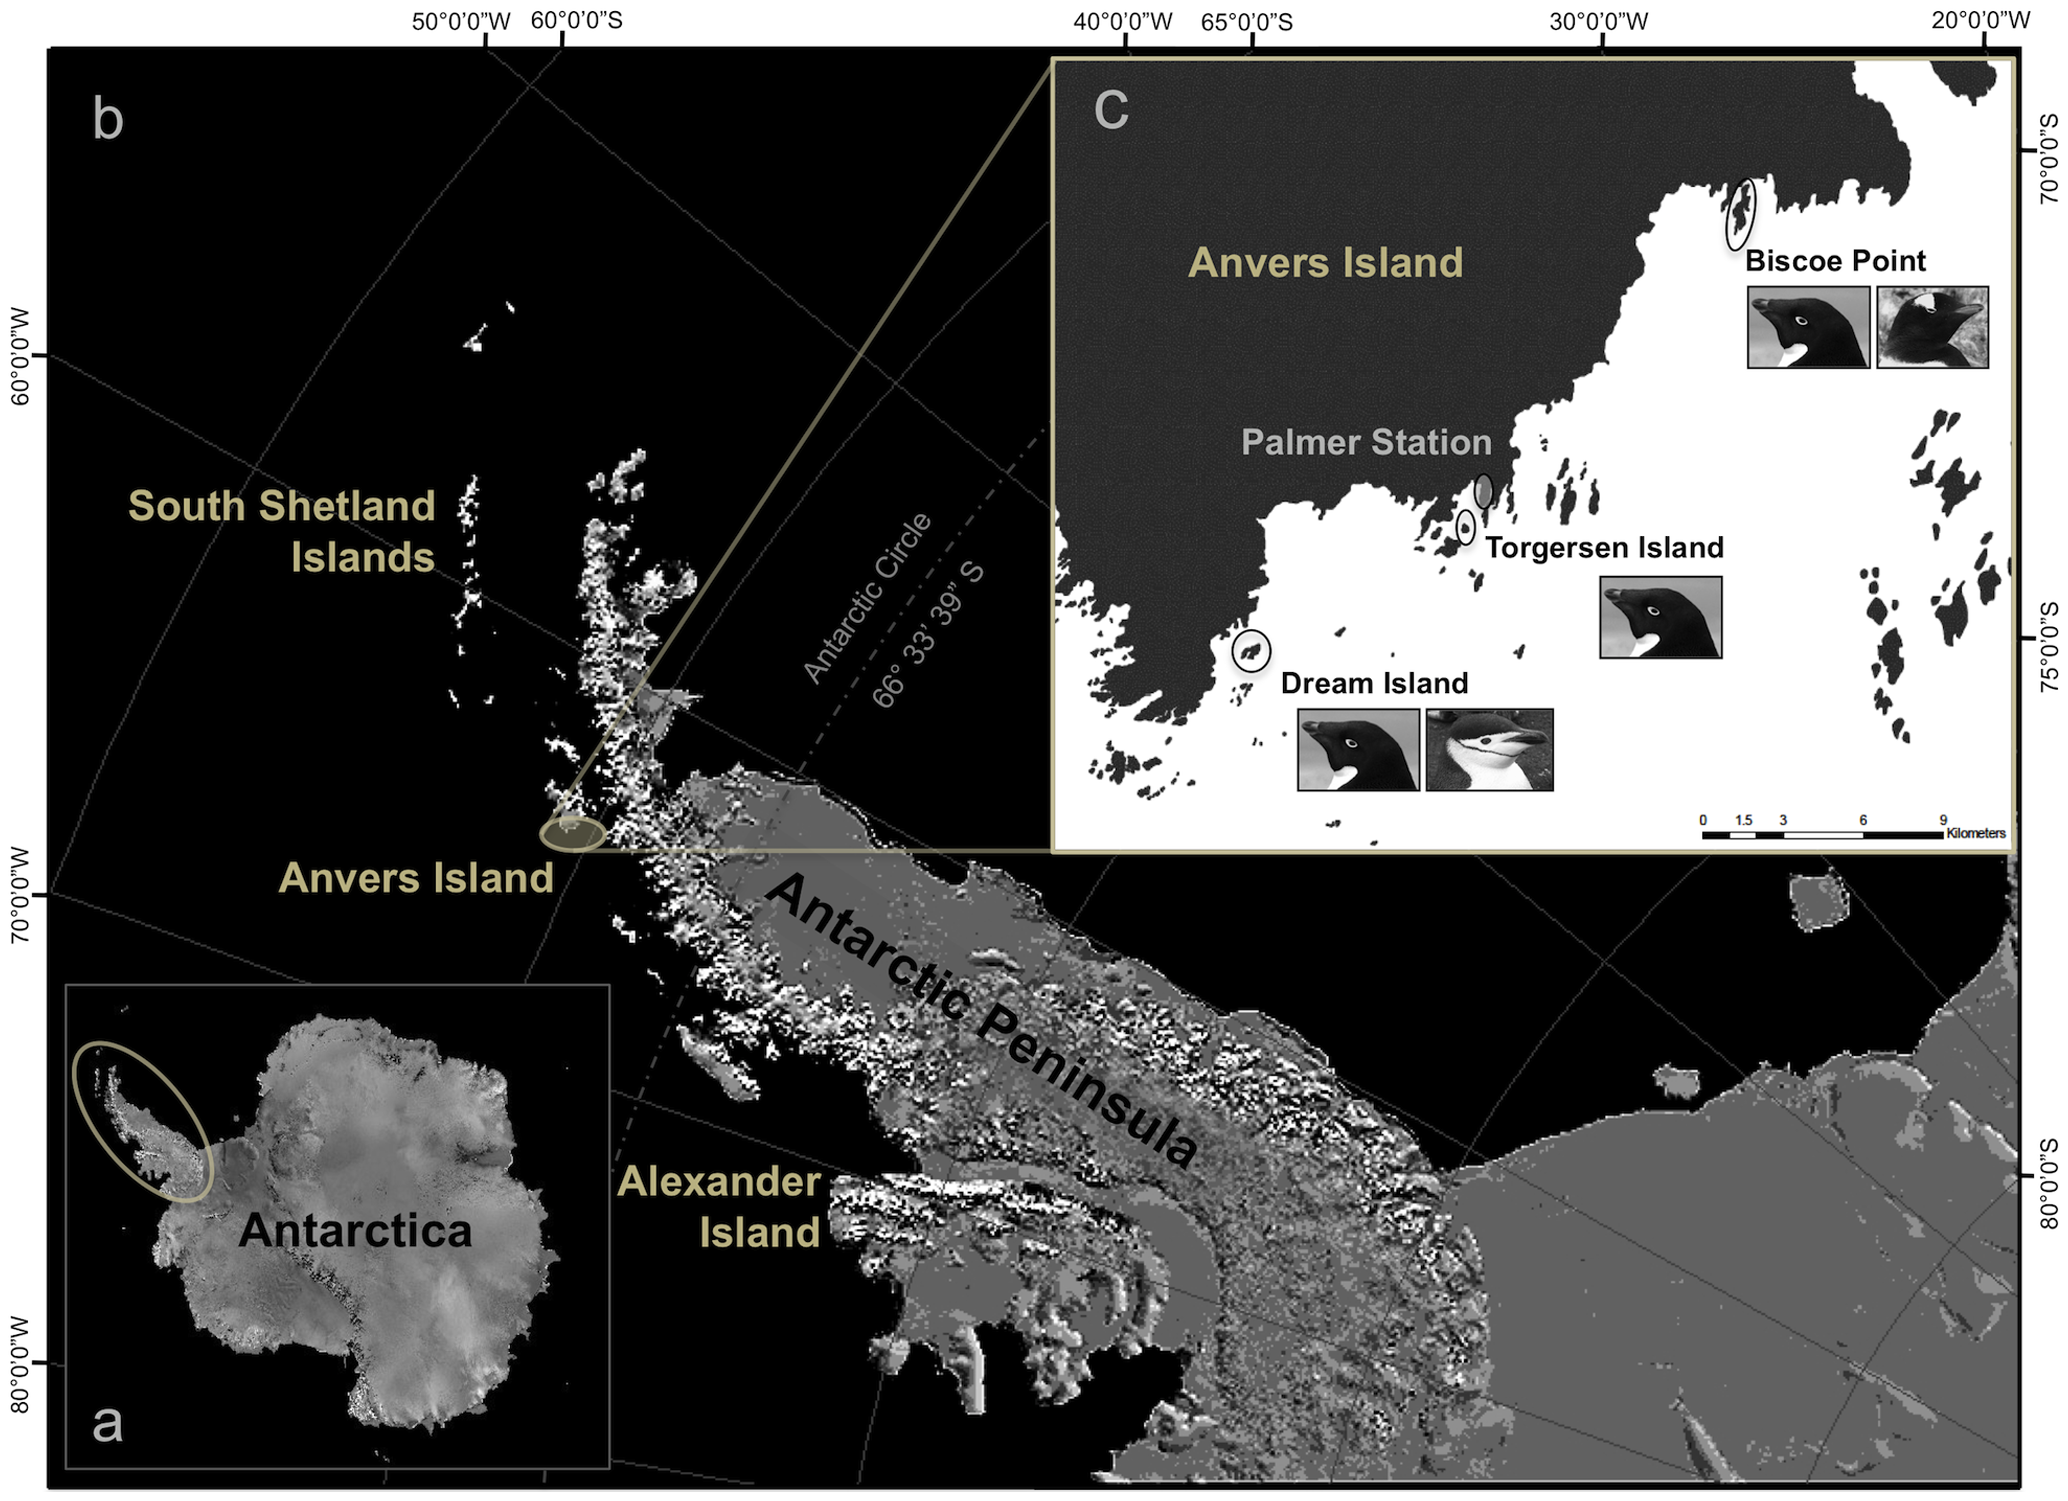
\includegraphics[width=0.8\linewidth]{images/antarctica-map}

\hypertarget{insights-from-data}{%
\subsection{Insights from data}\label{insights-from-data}}

This dataset is relatively simple, as there aren't too many variables to consider. But there are a reasonably large number of datapoints (individual penguins) making it possible to generate insights.

However, there are some specific and rather common problems in this data. Problems that we need to work through \emph{before} we can start to make any visuals or try to draw any conclusions. There are some problems with the variable names, there are some problems with some of the values. There are problems that one of the response variables isn't actually encoded on the dataset (we have to make it).

Today we are going to

\begin{itemize}
\item
  Formulate clear research questions
\item
  Import our dataset
\item
  Learn how to prepare our RStudio Project workspace
\item
  Learn how to clean, tidy and manipulate our data to allow tables, graphs and analyses to be run
\end{itemize}

Don't worry if you don't understand exactly what each function does at the moment, or struggle to remember every concept we are introduced to. We will cover these again, in lots more detail as we progress. The main point is to get familiar with our process for handling data and organising our projects.

\hypertarget{the-question}{%
\section{The Question?}\label{the-question}}

Imagine that you are a Penguin biologist. Chilly.

Imagine that you want to know more about the feeding habits of the different penguin species in the Antarctic. You also wish to characterise features such as bill morphology, and body size and compare them across species. Adelie and Chinstrap penguins are off-shore, shallow diving foragers, while Gentoo's feed closer inshort and are deep-divers. We might expect that we can find some features of Gentoo's that align with their different lifestyle/feeding habits.

With simple measuring techniques and identification skills we can sex the penguins, identify their species and take simple non-invasive measurements of features such as body size, flipper length and bill dimensions. You also recently read a paper about the ratios of different Nitrogen and Carbon isotopes in blood, and how these can be used to infer the types of prey that are forming an organism's diet.

\hypertarget{hypotheses}{%
\subsection{Hypotheses}\label{hypotheses}}

These hypotheses are fairly basic, we have not included directionality or specific expecations of the magnitude of the difference. This would come from doing more research on the subject area.

\begin{itemize}
\item
  The bill lengths/depths ratio to body size of Gentoo penguins will be different to Adelie and Chinstrap penguins.
\item
  Gentoo penguins will have a different N and carbon isotope ratio than Adelie and Chinstrap penguins.
\end{itemize}

\hypertarget{preparing-the-data}{%
\section{Preparing the data}\label{preparing-the-data}}

Imagine we have completed our practical study and have our data. The data is probably distributed in lots of places, originally notes collected in the field were probably on paper \& notebooks. Then someone will have taken time to transcribe those into a spreadsheet. This will almost certainly have been done by typing all the data in by hand.

It is very important for us to know how we would like our data to be organised at the end. We are going to learn how to organise data using the \emph{tidy} format\footnote{(\url{http://vita.had.co.nz/papers/tidy-data.pdf})}. This is because we are going to use the \texttt{tidyverse} packages by \citet{tidyverse2019}. This is an opinionated, but highly effective method for generating reproducible analyses with a wide-range of data manipulation tools. Tidy data is an easy format for computers to read.

\hypertarget{tidy-data}{%
\subsection{Tidy data}\label{tidy-data}}

Here `tidy' refers to a specific structure that lets us manipulate and visualise data with ease. In a tidy dataset each \emph{variable} is in one column and each row contains one \emph{observation}. Each cell of the table/spreadsheet contains the \emph{values}. Obe observation you might make about tidy data is it is quite long - it generates a lot of rows of data.

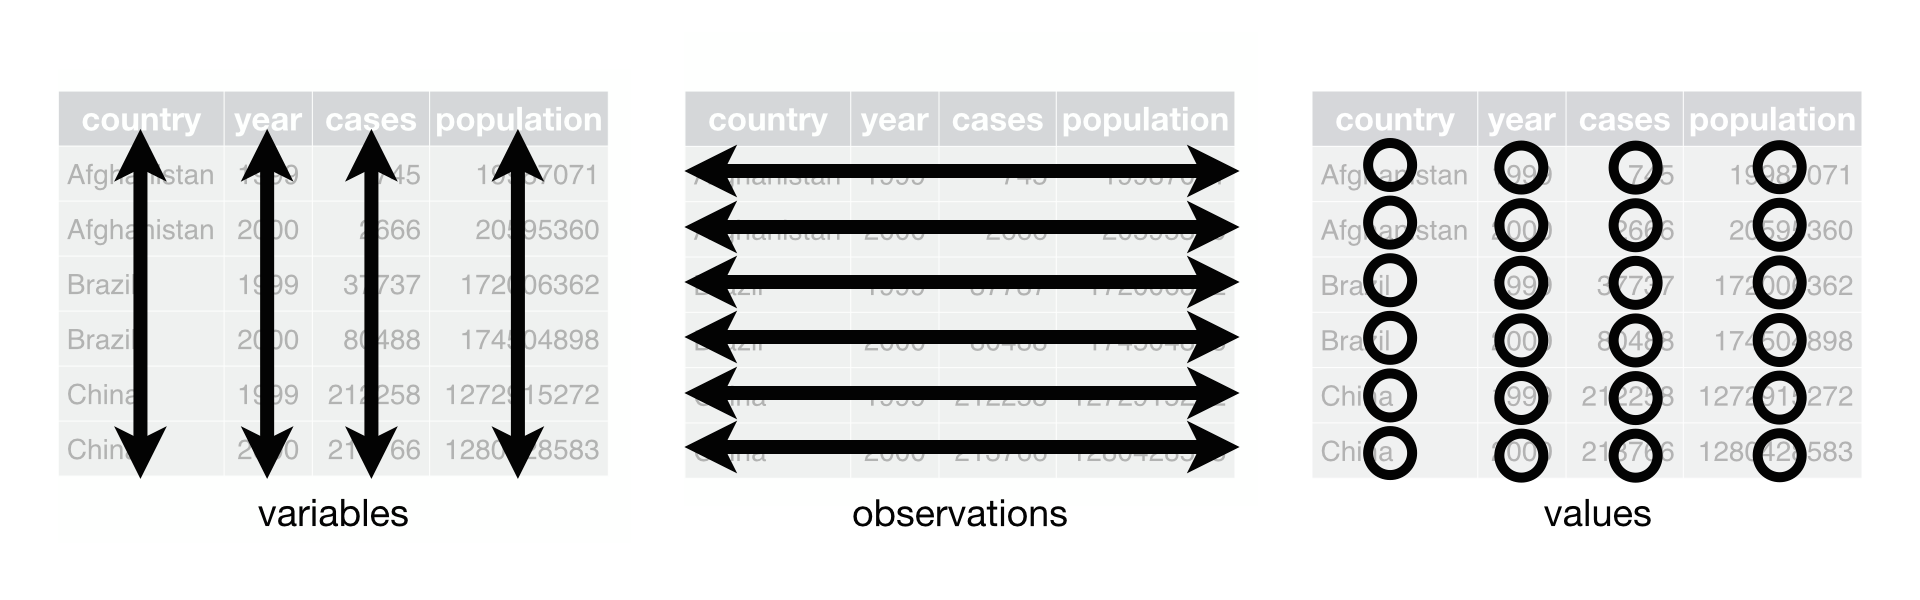
\includegraphics[width=0.8\linewidth]{images/tidy-1}

Typing data in, using any spreadsheet program (e.g.~Excel, Google sheets), if we type in the penguin data, we would make each row contain one observation about one penguin. If we made a second observation about a penguin (say in the next year of the study) it would get a new row in the dataset. You are probably thinking this is a lot of typing and a lot of repetition - and you are right! But this format allows the computer to easily make summaries at any level.

If the data we input to R is ``untidy'' then we have to spend a little bit of time tidying, we will explore this more later.

Once data has been typed up into a spreadsheet and double/triple-checked against the original paper records, then they are saved as a `comma-separated values (CSV)' file-type. These files are the simplest form of database, no coloured cells, no formulae, no text formatting. Each row is a row of the data, each value of a row (previously separate columns) is separated by a comma.

It is convenient to use something like Excel to type in our data - its much more usefully friendly than trying to tpye something in csv format. But we don't save files in the Excel format because they have a nasty habit of formatting or even losing data when the file gets large enough \footnote{\url{https://www.theguardian.com/politics/2020/oct/05/how-excel-may-have-caused-loss-of-16000-covid-tests-in-england}}.
If you need to add data to a csv file, you can always open it in an Excel-like program and add more information.

\begin{figure}
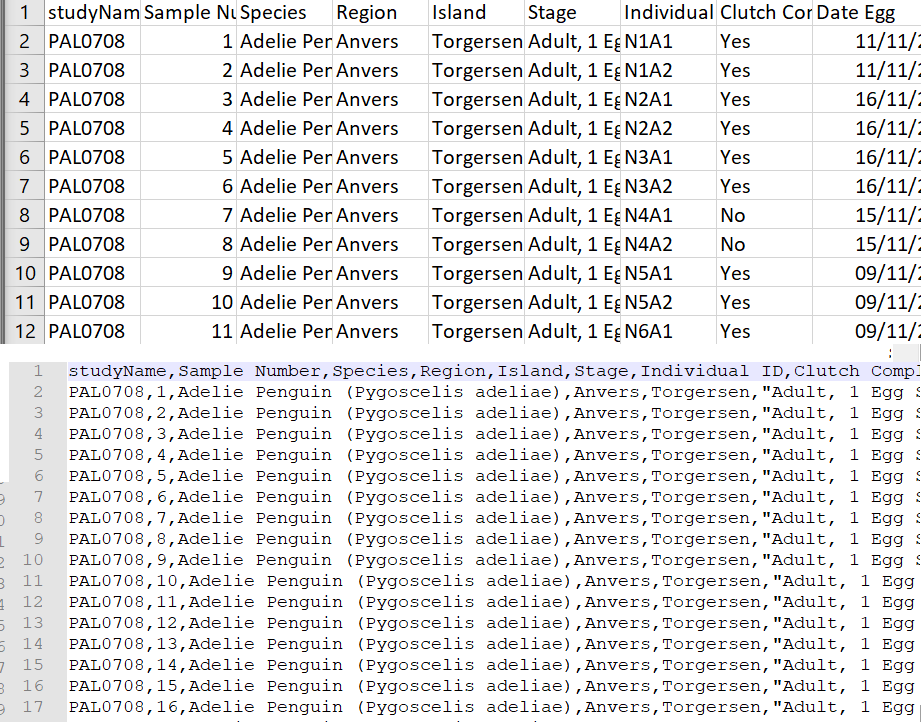
\includegraphics[width=0.8\linewidth]{images/excel_csv} \caption{Top image: Penguins data viewed in Excel, Bottom image: Penguins data in native csv format}\label{fig:unnamed-chunk-45}
\end{figure}

It is possible to import data into R in an Excel format, but I recommend sticking with csv formats. Any spreadsheet can be easily converted with the \emph{Save As..} command.

\hypertarget{the-dataset}{%
\subsection{The dataset}\label{the-dataset}}

For today's workshop we want to acquire the dataset to work on it. We can retrieve the file we need from here (\url{https://github.com/UEABIO/5023Y_Workshop/blob/main/data/penguins_raw.csv}).

\begin{figure}
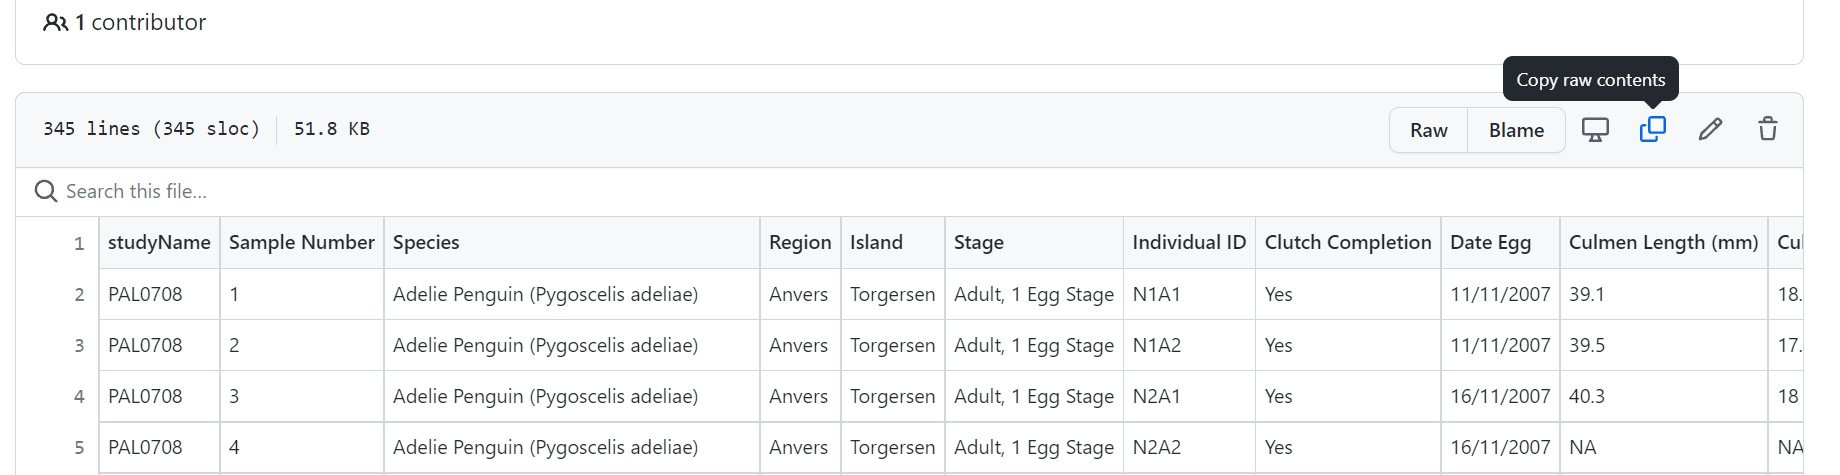
\includegraphics[width=1\linewidth]{images/penguin_github} \caption{Click on the copy raw contents button}\label{fig:unnamed-chunk-46}
\end{figure}

We then need to

\begin{enumerate}
\def\labelenumi{\arabic{enumi}.}
\item
  Select the copy raw contents button
\item
  Open a blank notepad
\item
  Paste the contents
\item
  Save the file as `penguin\_data.csv'
\item
  Open the newly saved file in Excel and take a look
\end{enumerate}

We can see a dataset with 345 rows (including the headers) and 17 variables

\begin{itemize}
\item
  \textbf{Study name}: an identifier for the year in which sets of observations were made
\item
  \textbf{Region}: the area in which the observation was recorded
\item
  \textbf{Island}: the specific island where the observation was recorded
\item
  \textbf{Stage}: Denotes reproductive stage of the penguin
\item
  \textbf{Individual} ID: the unique ID of the individual
\item
  \textbf{Clutch completion}: if the study nest observed with a full clutch e.g.~2 eggs
\item
  \textbf{Date egg}: the date at which the study nest observed with 1 egg
\item
  \textbf{Culmen length}: length of the dorsal ridge of the bird's bill (mm)
\item
  \textbf{Culmen depth}: depth of the dorsal ridge of the bird's bill (mm)
\item
  \textbf{Flipper Length}: length of bird's flipper (mm)
\item
  \textbf{Body Mass}: Bird's mass in (g)
\item
  \textbf{Sex}: Denotes the sex of the bird
\item
  \textbf{Delta 15N} : the ratio of stable Nitrogen isotopes 15N:14N from blood sample
\item
  \textbf{Delta 13C}: the ratio of stable Carbon isotopes 13C:12C from blood sample
\end{itemize}

\hypertarget{prepare-the-rstudio-workspace}{%
\section{Prepare the RStudio workspace}\label{prepare-the-rstudio-workspace}}

Now we should have our question, we understand more about where the data came from, and we have our data in a CSV format.

The next step of our workflow is to have a well organised project space. RStudio Cloud does a lot of the hard work for you, each new data project can be set up with its own Project space.

We will define a project as a series of linked questions that uses one (or sometimes several) datasets. For example a coursework assignment for a particular module would be its own project, or eventually your final year research project.

A Project will contain several files, possibly organised into sub-folders containing data, R scripts and final outputs. You might want to keep any information (wider reading) you have gathered that is relevant to your project.

Open the Week Two - workflow project on RStudio Cloud.

Within this project you will notice there is already one file \emph{.Rproj}. This is an R project file, this is a very useful feature, it interacts with R to tell it you are working in a very specific place on the computer (in this case the cloud server we have dialed into). It means R will automatically treat the location of your project file as the `working directory' and makes importing and exporting easier\footnote{More on projects can be found in the R4DS book (\url{https://r4ds.had.co.nz/workflow-projects.html})}.

\hypertarget{organise}{%
\subsection{Organise}\label{organise}}

Now we are going to organise our workspace, first its always a good first step to go to Tools \textgreater{} Project options and switch all of the options for saving and loading .Rdata to `No'

Then we create the following folders:

\begin{itemize}
\item
  data
\item
  scripts
\item
  figures
\end{itemize}

\begin{rmdwarning}
Make sure you type these \textbf{exactly} as printed here - remember
that to R is case-sensitive so `data' and `Data' are two different
things!
\end{rmdwarning}

Having these separate subfolders within our project helps keep things tidy, means it's harder to lose things, and lets you easily tell R exactly where to go to retrieve data.

Now do you remember where you saved the `penguin\_data.csv' file? I hope so!!! Go to the upload button in the Files tab of RStudio Cloud and tell it where the file is located on your local computer and upload it to the `data' folder you have made in your Project.

\begin{figure}
\includegraphics[width=0.8\linewidth]{images/project} \caption{An example of a typical R project set-up}\label{fig:unnamed-chunk-48}
\end{figure}

\hypertarget{create-a-new-r-script}{%
\subsection{Create a new R script}\label{create-a-new-r-script}}

Let's now create a new R script file in which we will write instructions and store comments for manipulating data, developing tables and figures. Use the File \textgreater{} New Script menu item and select an R Script.

Add the following:

\begin{Shaded}
\begin{Highlighting}[]
\CommentTok{\# An analysis of the bill dimensions of male and female Adelie, Gentoo and Chinstrap penguins. }

\CommentTok{\# Data first published in  Gorman, KB, TD Williams, and WR Fraser. 2014. “Ecological Sexual Dimorphism and Environmental Variability Within a Community of Antarctic Penguins (Genus Pygoscelis).” PLos One 9 (3): e90081. https://doi.org/10.1371/journal.pone.0090081.}
\end{Highlighting}
\end{Shaded}

Then load the following add-on package to the R script, just underneath these comments. Tidyverse isn't actually one package, but a bundle of many different packages that play well together - for example it \emph{includes} \texttt{ggplot2} which we used in the last session, so we don't have to call that separately

\begin{Shaded}
\begin{Highlighting}[]
\FunctionTok{library}\NormalTok{(tidyverse) }\CommentTok{\# tidy data packages}
\FunctionTok{library}\NormalTok{(janitor) }\CommentTok{\# cleaning variable names}
\FunctionTok{library}\NormalTok{(lubridate) }\CommentTok{\# make sure dates are processed properly}
\end{Highlighting}
\end{Shaded}

Now save this file in the scripts folder and call it \emph{penguin\_measurements.R}

\hypertarget{get-the-data-into-r}{%
\section{Get the data into R}\label{get-the-data-into-r}}

Now we are \emph{finally} ready to import the data into R.

Add the following code to your script, then starting at line 1 - ask your script to run in order, library function first as the \texttt{read\_csv()} function is from an add-on package \texttt{readr}

\begin{Shaded}
\begin{Highlighting}[]
\CommentTok{\# read in the data from the data folder in my project}
\NormalTok{penguins }\OtherTok{\textless{}{-}} \FunctionTok{read\_csv}\NormalTok{(}\StringTok{"data/penguins\_data.csv"}\NormalTok{)}
\end{Highlighting}
\end{Shaded}

\begin{verbatim}
Error!
\end{verbatim}

Houston we have a problem! We got an error!!! blah blah does not exist in current working directory

This usually happens if we told R to look in the wrong place, or didn't give it the correct name of what to look for. Can you spot what the mistake was?

Edit your existing line of script to replace it with the proper file name and run the command again.

\begin{Shaded}
\begin{Highlighting}[]
\CommentTok{\# read in the data from the data folder in my project}
\NormalTok{penguins }\OtherTok{\textless{}{-}} \FunctionTok{read\_csv}\NormalTok{(}\StringTok{"data/penguins\_data.csv"}\NormalTok{)}
\end{Highlighting}
\end{Shaded}

\begin{verbatim}
Parsed with column specification:
cols(
  studyName = col_character(),
  `Sample Number` = col_double(),
  Species = col_character(),
  Region = col_character(),
  Island = col_character(),
  Stage = col_character(),
  `Individual ID` = col_character(),
  `Clutch Completion` = col_character(),
  `Date Egg` = col_character(),
  `Culmen Length (mm)` = col_double(),
  `Culmen Depth (mm)` = col_double(),
  `Flipper Length (mm)` = col_double(),
  `Body Mass (g)` = col_character(),
  Sex = col_character(),
  `Delta 15 N (o/oo)` = col_double(),
  `Delta 13 C (o/oo)` = col_double(),
  Comments = col_character()
)
\end{verbatim}

Great, no error this time, the \texttt{read\_csv()} function has read the data and we \textless- assigned this data to the object \texttt{penguins}. If you look in the environment pane you should see the object \texttt{penguins}.

The lines printed in the R console tell us the names of the columns that were identified in the file and the type of variable R thinks it is

\begin{itemize}
\item
  \texttt{col\_character()} means the column contains letters or words
\item
  \texttt{col\_double()} means the column contains numbers
\end{itemize}

\begin{rmdquestion}
Have a look - do all of these seem correct to you? If not we should fix
these, and we will get onto that in a little bit.
\end{rmdquestion}

\hypertarget{view-and-refine}{%
\subsection{View and refine}\label{view-and-refine}}

So we know our data is in R, and we know the columns and names have been imported. But we still don't know whether all of our values imported, or whether it captured all the rows.

There are lots of different ways to view and check data. One useful method is \texttt{glimpse}

\begin{Shaded}
\begin{Highlighting}[]
\CommentTok{\# check the structure of the data}
\FunctionTok{glimpse}\NormalTok{(penguins)}
\end{Highlighting}
\end{Shaded}

When we run \texttt{glimpse()} we get several lines of output. The number of observations ``rows'', the number of variables ``columns''. Check this against the csv file you have - they should be the same. In the next lines we see variable names and the type of data.

We should be able to see by now, that all is not well!!! \texttt{Body\ Mass\ (g)} is being treated as character (string), as is \texttt{Date\ Egg}, meaning R thinks these contain letters and words instead of numbers and dates.

Other ways to view the data

\begin{itemize}
\item
  type \texttt{penguins} into the Console
\item
  type \texttt{view(penguins)} this will open a spreadsheet in a new tab
\item
  type \texttt{head(penguins)} will show the first 10 lines of the data, rather than the whole dataset
\end{itemize}

\begin{quote}
**Note - \texttt{view()} lets you do cool stuff like reorder rows and quickly scroll through the dataset without affecting the underlying data.
\end{quote}

\hypertarget{data-management}{%
\subsection{Data management}\label{data-management}}

We've imported the data, checked it and found some inconsistencies.

This is where we start to use some of the core functions from \texttt{tidyverse}.

If R thinks \texttt{Body\ Mass\ (g)} is a character variable, then it probably contains some words as well as numbers. So let's have a look at this and compare it to a variable which has been processed correctly

\begin{Shaded}
\begin{Highlighting}[]
\CommentTok{\# get the first 10 rows of the Flipper Length and Body Mass variables}
\NormalTok{penguins }\SpecialCharTok{\%\textgreater{}\%} 
  \FunctionTok{select}\NormalTok{(}\StringTok{\textasciigrave{}}\AttributeTok{Flipper Length (mm)}\StringTok{\textasciigrave{}}\NormalTok{, }
         \StringTok{\textasciigrave{}}\AttributeTok{Body Mass (g)}\StringTok{\textasciigrave{}}\NormalTok{) }\SpecialCharTok{\%\textgreater{}\%} 
  \FunctionTok{head}\NormalTok{(}\DecValTok{10}\NormalTok{) }\CommentTok{\# 10 rows}
\end{Highlighting}
\end{Shaded}

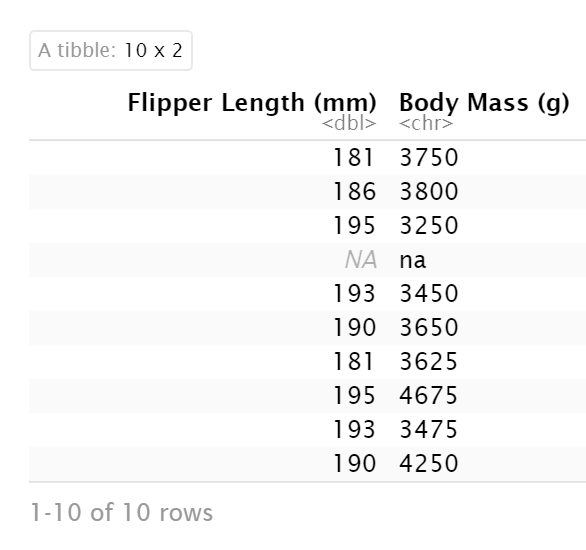
\includegraphics[width=0.8\linewidth]{images/NA}

\begin{quote}
**Note - What is the \%\textgreater\% ??? It's known as a pipe. It sends the results of one line of code to the next. So the data penguins is sent to the \texttt{select} function which picks only those variables we want. The result of this is then sent to the \texttt{head} function which with the argument for number of rows set to 10, prints the top 10 rows.
\end{quote}

\begin{quote}
The other way to write this series of functions would be to use brackets and the rules of BODMAS:
\end{quote}

\begin{verbatim}
head(select(penguins, `Flipper Length (mm)`, `Body Mass (g)`),10)
\end{verbatim}

\begin{quote}
Hopefully you agree that the pipes make the code a lot more human-reader friendly. More on pipes later
\end{quote}

So what's the problem with our data? in the Flipper length variable, missing observations have been correctly marked as \texttt{NA} signifying missing data. R can handle missing data just fine. However, in thew Body mass variable, it looks as though someone has actually typed ``na'' in observations where the data is missing. Here R has failed to recognise an \texttt{NA} and has read it as a word instead. This is because \texttt{read\_csv()} looks for gaps or \texttt{NA} but not ``na''.

No problem this is an easy fix. Head back to your script and make the following edit the line for data importing

\begin{Shaded}
\begin{Highlighting}[]
\CommentTok{\# read in the penguins data, specify that NA strings can be "na" or "NA"}
\NormalTok{penguins }\OtherTok{\textless{}{-}} \FunctionTok{read\_csv}\NormalTok{(}\StringTok{"data/penguin\_data.csv"}\NormalTok{, }\AttributeTok{na=}\FunctionTok{c}\NormalTok{(}\StringTok{"na"}\NormalTok{,}\StringTok{"NA"}\NormalTok{))}
\end{Highlighting}
\end{Shaded}

Now re-check your data using the same lines of code from before.
All ok now?

\hypertarget{dataframes-and-tibbles}{%
\section{Dataframes and tibbles}\label{dataframes-and-tibbles}}

A quick sidebar on how R stores data. When we imported the data into R it ws put into an object called a \textbf{tibble} which is a type of \textbf{dataframe}.

Let's have a quick go at making our own \textbf{tibble} from scratch.

Make a new script called `TibbleTrouble.R' in the scripts folder as before.

At the top of this new script put

\begin{Shaded}
\begin{Highlighting}[]
\CommentTok{\# just me messing about making tibbles}

\CommentTok{\# libraries}
\FunctionTok{library}\NormalTok{(tidyverse)}

\CommentTok{\# make some variables, when we have a one dimensional object like this it is known as an atomic vector!}
\NormalTok{person }\OtherTok{\textless{}{-}} \FunctionTok{c}\NormalTok{(}\StringTok{"Mark"}\NormalTok{, }\StringTok{"Phil"}\NormalTok{, }\StringTok{"Becky"}\NormalTok{, }\StringTok{"Tony"}\NormalTok{)}
\NormalTok{hobby }\OtherTok{\textless{}{-}} \FunctionTok{c}\NormalTok{(}\StringTok{"kickboxing"}\NormalTok{, }\StringTok{"coding"}\NormalTok{, }\StringTok{"dog walking"}\NormalTok{, }\StringTok{"car boot sales"}\NormalTok{)}
\NormalTok{awesomeness }\OtherTok{\textless{}{-}} \FunctionTok{c}\NormalTok{(}\DecValTok{1}\NormalTok{,}\DecValTok{100}\NormalTok{,}\DecValTok{1}\NormalTok{,}\DecValTok{1}\NormalTok{)}
\end{Highlighting}
\end{Shaded}

The function \texttt{c} lets you `concatenate' or link each of these arguments together into a single vector.

Now we put these vectors together, where they become the variables in a new tibble

\begin{Shaded}
\begin{Highlighting}[]
\CommentTok{\# make a tibble}
\NormalTok{my\_data }\OtherTok{\textless{}{-}} \FunctionTok{tibble}\NormalTok{(person, hobby, awesomeness)}
\NormalTok{my\_data}
\end{Highlighting}
\end{Shaded}

\begin{verbatim}
# A tibble: 4 x 3
  person hobby          awesomeness
  <chr>  <chr>                <dbl>
1 Mark   kickboxing               1
2 Phil   coding                 100
3 Becky  dog walking              1
4 Tony   car boot sales           1
\end{verbatim}

Have a go at messing about with your script and figure out what each of these does, add comments and save your script.

\begin{Shaded}
\begin{Highlighting}[]
\CommentTok{\# Some R functions for looking at tibbles and dataframes I will comment next to each one with what it does}

\FunctionTok{head}\NormalTok{(my\_data, }\AttributeTok{n=}\DecValTok{2}\NormalTok{)}
\FunctionTok{tail}\NormalTok{(my\_data, }\AttributeTok{n=}\DecValTok{1}\NormalTok{)}
\FunctionTok{nrow}\NormalTok{(my\_data)}
\FunctionTok{ncol}\NormalTok{(my\_data)}
\FunctionTok{colnames}\NormalTok{(my\_data)}
\FunctionTok{view}\NormalTok{(my\_data)}
\FunctionTok{glimpse}\NormalTok{(my\_data)}
\FunctionTok{str}\NormalTok{(my\_data)}
\end{Highlighting}
\end{Shaded}

\hypertarget{clean-and-tidy}{%
\section{Clean and tidy}\label{clean-and-tidy}}

Back to your penguins script.

We have checked the data imported correctly, now its time to \emph{clean and tidy} the data.

\hypertarget{tidy}{%
\subsection{Tidy}\label{tidy}}

In this example our data is already in \texttt{tidy} format i.e.~one observation per row. We will cover what to do if data isn't tidy later.

\hypertarget{clean}{%
\subsection{Clean}\label{clean}}

Here are a few things we might want to do to our data to make it `clean'.

\begin{itemize}
\item
  Refine variable names
\item
  Format dates and times
\item
  Rename some values
\item
  Check for any duplicate records
\item
  Check for any implausible data or typos
\item
  Check and deal with missing values
\end{itemize}

\begin{quote}
**Note - Remember because we are doing everything in a script, the original data remains unchanged. This means we have data integrity, and a clear record of what we did to tidy and clean a dataset in order to produce summaries and data visuals
\end{quote}

\hypertarget{refine-variable-names}{%
\subsection{Refine variable names}\label{refine-variable-names}}

Often we might want to change the names of our variables. They might be non-intuitive, or too long. Our data has a couple of issues:

\begin{itemize}
\item
  Some of the names contain spaces
\item
  Some of the names contain brackets
\end{itemize}

Let's correct these quickly

\begin{Shaded}
\begin{Highlighting}[]
\CommentTok{\#clean all variable names to snake\_case using the clean\_names function from the janitor package}
\CommentTok{\# note we are using assign \textless{}{-} to overwrite the old version of penguins with a version that has updated names}
\CommentTok{\# this changes the data in our R workspace but not the original csv file}

\NormalTok{penguins }\OtherTok{\textless{}{-}}\NormalTok{ penguins }\SpecialCharTok{\%\textgreater{}\%} \CommentTok{\#}
\NormalTok{  janitor}\SpecialCharTok{::}\FunctionTok{clean\_names}\NormalTok{()}

\FunctionTok{colnames}\NormalTok{(penguins) }\CommentTok{\# quickly check the new variable names}
\end{Highlighting}
\end{Shaded}

\begin{quote}
**Note - in this example you can see that I put the name of the package janitor, in front of the function \texttt{clean\_names}. But if I have already loaded the package with library(janitor) then this isn't strictly necessary and penguins \%\textgreater\% clean\_names() would also have worked just fine. So why do this? Remember when we loaded the tidyverse package - we got a warning about conflicts - this was because two of our packages \texttt{dplyr} and \texttt{stats} have functions that are different, but share the same name. But we can make sure we call the one we want by specifying which package we are calling a function from. We don't need to do this very often, but it's good to know.
\end{quote}

\begin{verbatim}
> library(tidyverse)
-- Attaching packages --------------------------------------- tidyverse 1.3.0 --
v ggplot2 3.3.2     v purrr   0.3.4
v tibble  3.0.4     v dplyr   1.0.2
v tidyr   1.1.2     v stringr 1.4.0
v readr   1.3.1     v forcats 0.5.0
-- Conflicts ------------------------------------------ tidyverse_conflicts() --
x dplyr::filter() masks stats::filter()
x dplyr::lag()    masks stats::lag()
\end{verbatim}

The \texttt{clean\_names} function quickly converts all variable names into snake case. The N and C blood isotope ratio names are still quite long though, so let's clean those with \texttt{dplyr::rename()} where ``new\_name'' = ``old\_name''.

\begin{Shaded}
\begin{Highlighting}[]
\CommentTok{\# shorten the variable names for N and C isotope blood samples}

\NormalTok{penguins }\OtherTok{\textless{}{-}}\NormalTok{ penguins }\SpecialCharTok{\%\textgreater{}\%} 
  \FunctionTok{rename}\NormalTok{(}\StringTok{"delta\_15n"}\OtherTok{=}\StringTok{"delta\_15\_n\_o\_oo"}\NormalTok{,  }\CommentTok{\# use rename from the dplyr package}
         \StringTok{"delta\_13c"}\OtherTok{=}\StringTok{"delat\_13\_c\_o\_oo"}\NormalTok{)}
\end{Highlighting}
\end{Shaded}

\hypertarget{dates}{%
\subsection{Dates}\label{dates}}

We can also see there is a \texttt{date\_egg} variable. If you check it (using any of the new functions you have learned), you should see that it all looks like its been inputted correctly, but R is treating it as words, rather than assigning it a date value. We can fix that with the \texttt{lubridate} package. If we use the function \texttt{dmy} then we tell R this is date data in date/month/year format.

\begin{Shaded}
\begin{Highlighting}[]
\CommentTok{\# use dmy from stringr package to encode date properly}
\NormalTok{penguins }\OtherTok{\textless{}{-}}\NormalTok{ penguins }\SpecialCharTok{\%\textgreater{}\%} 
  \FunctionTok{mutate}\NormalTok{(}\AttributeTok{date\_egg\_proper=}\FunctionTok{dmy}\NormalTok{(date\_egg))}
\end{Highlighting}
\end{Shaded}

\begin{rmdquestion}
What is the deliberate mistake in my code comment above? By now you may
have picked up there are the odd mistakes (possibly some non-deliberate
ones) - to make sure you aren't just copy-pasting on autpilot.
\end{rmdquestion}

Here we use the \texttt{mutate} function from \texttt{dplyr} to create a new variable called \texttt{date\_egg\_proper} based on the output of converting the characters in \texttt{date\_egg} to date format. The original variable is left intact, if we had specified the ``new'' variable was also called \texttt{date\_egg} then it would have overwritten the original variable.

\hypertarget{rename-some-values}{%
\subsection{Rename some values}\label{rename-some-values}}

Sometimes we may want to rename the values in our variables in order to make a shorthand that is easier to follow.

\begin{Shaded}
\begin{Highlighting}[]
\CommentTok{\# use mutate and case\_when for an if{-}else statement that changes the names of the values in a variable}
\NormalTok{penguins }\OtherTok{\textless{}{-}}\NormalTok{ penguins }\SpecialCharTok{\%\textgreater{}\%} 
  \FunctionTok{mutate}\NormalTok{(}\AttributeTok{species =} \FunctionTok{case\_when}\NormalTok{(species }\SpecialCharTok{==} \StringTok{"Adelie Penguin (Pygoscelis adeliae)"} \SpecialCharTok{\textasciitilde{}} \StringTok{"Adelie"}\NormalTok{,}
\NormalTok{                             species }\SpecialCharTok{==} \StringTok{"Gentoo penguin (Pygoscelis papua)"} \SpecialCharTok{\textasciitilde{}} \StringTok{"Gentoo"}\NormalTok{,}
\NormalTok{                             species }\SpecialCharTok{==} \StringTok{"Chinstrap penguin (Pygoscelis antarctica)"} \SpecialCharTok{\textasciitilde{}} \StringTok{"Chinstrap"}\NormalTok{))}
\end{Highlighting}
\end{Shaded}

\hypertarget{check-for-duplication}{%
\subsection{Check for duplication}\label{check-for-duplication}}

It is very easy when inputting data to make mistakes, copy something in twice for example, or if someone did a lot of copy-pasting to assemble a spreadsheet (yikes!). We can check this pretty quickly

\begin{Shaded}
\begin{Highlighting}[]
\CommentTok{\# check for duplicate rows in the data}
\NormalTok{penguins }\SpecialCharTok{\%\textgreater{}\%} 
  \FunctionTok{duplicated}\NormalTok{() }\SpecialCharTok{\%\textgreater{}\%} \CommentTok{\# produces a list of TRUE/FALSE statements for duplicated or not}
  \FunctionTok{sum}\NormalTok{() }\CommentTok{\# sums all the TRUE statements}
\end{Highlighting}
\end{Shaded}

\begin{verbatim}
[1] 0
\end{verbatim}

Great!

\hypertarget{check-for-typos-or-implausible-values}{%
\subsection{Check for typos or implausible values}\label{check-for-typos-or-implausible-values}}

We can also explore our data for very obvious typos by checking for implausibly small or large values

\begin{Shaded}
\begin{Highlighting}[]
\CommentTok{\# use summarise to make calculations}
\NormalTok{penguins }\SpecialCharTok{\%\textgreater{}\%} 
  \FunctionTok{summarise}\NormalTok{(}\AttributeTok{min=}\FunctionTok{min}\NormalTok{(body\_mass\_g, }\AttributeTok{na.rm=}\ConstantTok{TRUE}\NormalTok{), }
            \AttributeTok{max=}\FunctionTok{max}\NormalTok{(body\_mass\_g, }\AttributeTok{na.rm=}\ConstantTok{TRUE}\NormalTok{))}
\end{Highlighting}
\end{Shaded}

The minimum weight for our penguins is 2.7kg, and the max is 6.3kg - not outrageous. If the min had come out at 27g we might have been suspicious. We will use \texttt{summarise} again to calculate other metrics in the future.

\begin{quote}
**Note - our first data insight, the difference the smallest adult penguin in our dataset is nearly half the size of the largest penguin.
\end{quote}

We can also look for typos by asking R to produce all of the distinct values in a variable. This is more useful for categorical data, where we expect there to be only a few distinct categories

\begin{Shaded}
\begin{Highlighting}[]
\NormalTok{penguins }\SpecialCharTok{\%\textgreater{}\%} 
  \FunctionTok{distinct}\NormalTok{(sex)}
\end{Highlighting}
\end{Shaded}

Here if someone had mistyped e.g.~`FMALE' it would be obvious. We could do the same thing (and probably should have before we changed the names) for species.

\hypertarget{missing-values-na}{%
\subsection{Missing values: NA}\label{missing-values-na}}

There are multiple ways to check for missing values in our data

\begin{Shaded}
\begin{Highlighting}[]
\CommentTok{\# Get a sum of how many observations are missing in our dataframe}
\NormalTok{penguins }\SpecialCharTok{\%\textgreater{}\%} 
  \FunctionTok{is.na}\NormalTok{() }\SpecialCharTok{\%\textgreater{}\%} 
  \FunctionTok{sum}\NormalTok{()}
\end{Highlighting}
\end{Shaded}

But this doesn't tell us where these are, fortunately the function \texttt{summary} does this easily

\begin{Shaded}
\begin{Highlighting}[]
\CommentTok{\# produce a summary of our data}
\FunctionTok{summary}\NormalTok{(penguins)}
\end{Highlighting}
\end{Shaded}

This provides a quick breakdown of the max and min for all numeric variables, as well as a list of how many missing observations there are for each one. As we can see there appear to be two missing observations for measurements in body mass, bill lengths, flipper lengths and several more for blood measures. We don't know for sure without inspecting our data further, \emph{but} it is likely that the two birds are missing multiple measurements, and that several more were measured but didn't have their blood drawn.

We will leave the NA's alone for now, but it's useful to know how many we have.

We've now got a clean \& tidy dataset!!

\hypertarget{summing-up}{%
\section{Summing up}\label{summing-up}}

\hypertarget{what-we-learned}{%
\subsection{What we learned}\label{what-we-learned}}

There was a lot of preparation here, and we haven't really got close to make any major insights. But you have:

\begin{itemize}
\item
  Organised your project space
\item
  Dealt with file formats
\item
  Put data into a specific location and imported into R
\item
  Checked the data import
\item
  Cleaned and tidied the data
\end{itemize}

You have also been introduced to the \texttt{tidyverse} and two of its packages

\begin{itemize}
\item
  \texttt{readr} \citet{R-readr}
\item
  \texttt{dplyr} \citet{R-dplyr}
\end{itemize}

As well as:

\begin{itemize}
\item
  \texttt{janitor} \citet{R-janitor}
\item
  \texttt{lubridate} \citet{R-lubridate}
\end{itemize}

\hypertarget{quitting-1}{%
\subsection{Quitting}\label{quitting-1}}

\begin{rmdwarning}
Remember to \textbf{save} your RScript before you leave. And ideally
don't save your .Rdata!
\end{rmdwarning}

\begin{itemize}
\item
  Close your RStudio Cloud Browser
\item
  Go to Blackboard to complete this week's quiz!
\end{itemize}

\hypertarget{workflow-part-two-week-three}{%
\chapter{Workflow Part Two: Week Three}\label{workflow-part-two-week-three}}

Last week we worked through the journey of importing and tidying data to produce a clean dataset.

It's important to remember what questions you have about the data collected, and to make an outline about what you want to do.

\begin{rmdquestion}
Now is a good time to think about what figures might we want to produce
from our data?

We are mostly interested in observable `differences' between our three
penguin species. What sort of figures might illustrate that?

Sometimes it's good to get a pen/pencil and paper - and sketch the
figure you might want to make.
\end{rmdquestion}

\hypertarget{initial-insights}{%
\section{Initial insights}\label{initial-insights}}

Let's start with some basic insights, perhaps by focusing on further questions about specific variables.

\begin{itemize}
\item
  How many penguins were observed?
\item
  How many Adelie, Gentoo and Chinstrap penguins
\item
  What is the distribution of morphologies such as bill length, body size, flipper length
\end{itemize}

Some of these are very simple in that they are summaries of single variables. Some are more complex, like evaluating the numbers of males and females which are the two groups in the sex variable.

These are `safety-checking' insights. You might already know the answers to some of these questions because you may have been responsible for collecting the data. Checking your answers against what you expect is a good way to check your data has been cleaned properly.

\hypertarget{numbers-and-sex-of-the-penguins}{%
\section{Numbers and sex of the penguins}\label{numbers-and-sex-of-the-penguins}}

\begin{Shaded}
\begin{Highlighting}[]
\CommentTok{\# how many observations of penguins were made}

\NormalTok{penguins }\SpecialCharTok{\%\textgreater{}\%} 
  \FunctionTok{summarise}\NormalTok{(}\FunctionTok{n}\NormalTok{())}

\CommentTok{\# but there are multiple observations of penguins across different years}
\CommentTok{\# n\_distinct deals with this}

\NormalTok{penguins }\SpecialCharTok{\%\textgreater{}\%} 
  \FunctionTok{summarise}\NormalTok{(}\FunctionTok{n\_distinct}\NormalTok{(individual\_id))}
\end{Highlighting}
\end{Shaded}

The answer we get is that there are 190 different penguins observed across our multi-year study.

This answer is provided in a tibble, but the variable name is an ugly composition of the functions applied, but we can modify the code

\begin{Shaded}
\begin{Highlighting}[]
\NormalTok{penguins }\SpecialCharTok{\%\textgreater{}\%} 
  \FunctionTok{summarise}\NormalTok{(}\AttributeTok{num\_penguin\_id=}\FunctionTok{n\_distinct}\NormalTok{(individual\_id))}
\end{Highlighting}
\end{Shaded}

How about the number of penguins observed from each species?

\begin{Shaded}
\begin{Highlighting}[]
\NormalTok{penguins }\SpecialCharTok{\%\textgreater{}\%} 
  \FunctionTok{group\_by}\NormalTok{(species) }\SpecialCharTok{\%\textgreater{}\%} \CommentTok{\# ask for distinct counts in each species}
  \FunctionTok{summarise}\NormalTok{(}\AttributeTok{num\_penguin\_id=}\FunctionTok{n\_distinct}\NormalTok{(individual\_id))}
\end{Highlighting}
\end{Shaded}

By adding the \texttt{group\_by} function we tell R to apply any subsequent functions separately according to the group specified. Let's do this again for male and female penguins

\begin{Shaded}
\begin{Highlighting}[]
\NormalTok{penguins }\SpecialCharTok{\%\textgreater{}\%} 
  \FunctionTok{group\_by}\NormalTok{(sex) }\SpecialCharTok{\%\textgreater{}\%} \CommentTok{\# ask for distinct counts in each species}
  \FunctionTok{summarise}\NormalTok{(}\AttributeTok{num\_penguin\_id=}\FunctionTok{n\_distinct}\NormalTok{(individual\_id))}
\end{Highlighting}
\end{Shaded}

Now what about the number of female Gentoo penguins?

\begin{Shaded}
\begin{Highlighting}[]
\NormalTok{penguins }\SpecialCharTok{\%\textgreater{}\%} 
  \FunctionTok{group\_by}\NormalTok{(sex, species) }\SpecialCharTok{\%\textgreater{}\%} \CommentTok{\# ask for distinct counts in each species}
  \FunctionTok{summarise}\NormalTok{(}\AttributeTok{num\_penguin\_id=}\FunctionTok{n\_distinct}\NormalTok{(individual\_id))}
\end{Highlighting}
\end{Shaded}

Now we have a table that shows each combination of penguin species by sex, we can see for example that 65 unique Male Adelie penguins were observed in our study. We can also see that for 6 Adelie and 5 Gentoo penguins, sex was not recorded.

\begin{quote}
**Note - You have just had a crash course in using the \texttt{pipe} and \texttt{dplyr} to produce quick data summaries. Have a go at making some other summaries of your data, perhaps the numbers of penguins by island or region. Try some combinations.
\end{quote}

\hypertarget{making-a-simple-figure}{%
\subsection{Making a simple figure}\label{making-a-simple-figure}}

Let's translate some of our simple summaries into graphs.

\begin{Shaded}
\begin{Highlighting}[]
\CommentTok{\# make summary data and assign to an object with a sensible name we can use}
\NormalTok{penguin\_species\_sex }\OtherTok{\textless{}{-}}\NormalTok{ penguins }\SpecialCharTok{\%\textgreater{}\%} 
  \FunctionTok{group\_by}\NormalTok{(sex, species) }\SpecialCharTok{\%\textgreater{}\%} \CommentTok{\# ask for distinct counts in each species}
  \FunctionTok{summarise}\NormalTok{(}\AttributeTok{num\_penguin\_id=}\FunctionTok{n\_distinct}\NormalTok{(individual\_id)) }\SpecialCharTok{\%\textgreater{}\%} 
  \FunctionTok{drop\_na}\NormalTok{() }\CommentTok{\# remove the missing data}
\end{Highlighting}
\end{Shaded}

\begin{Shaded}
\begin{Highlighting}[]
\CommentTok{\# basic ggplot function to make a stacked barplot}
\NormalTok{penguin\_species\_sex }\SpecialCharTok{\%\textgreater{}\%} 
  \FunctionTok{ggplot}\NormalTok{(}\FunctionTok{aes}\NormalTok{(}\AttributeTok{x=}\NormalTok{species, }
             \AttributeTok{y=}\NormalTok{num\_penguin\_id, }
             \AttributeTok{fill=}\NormalTok{sex))}\SpecialCharTok{+}
  \FunctionTok{geom\_col}\NormalTok{()}
\end{Highlighting}
\end{Shaded}

\begin{figure}
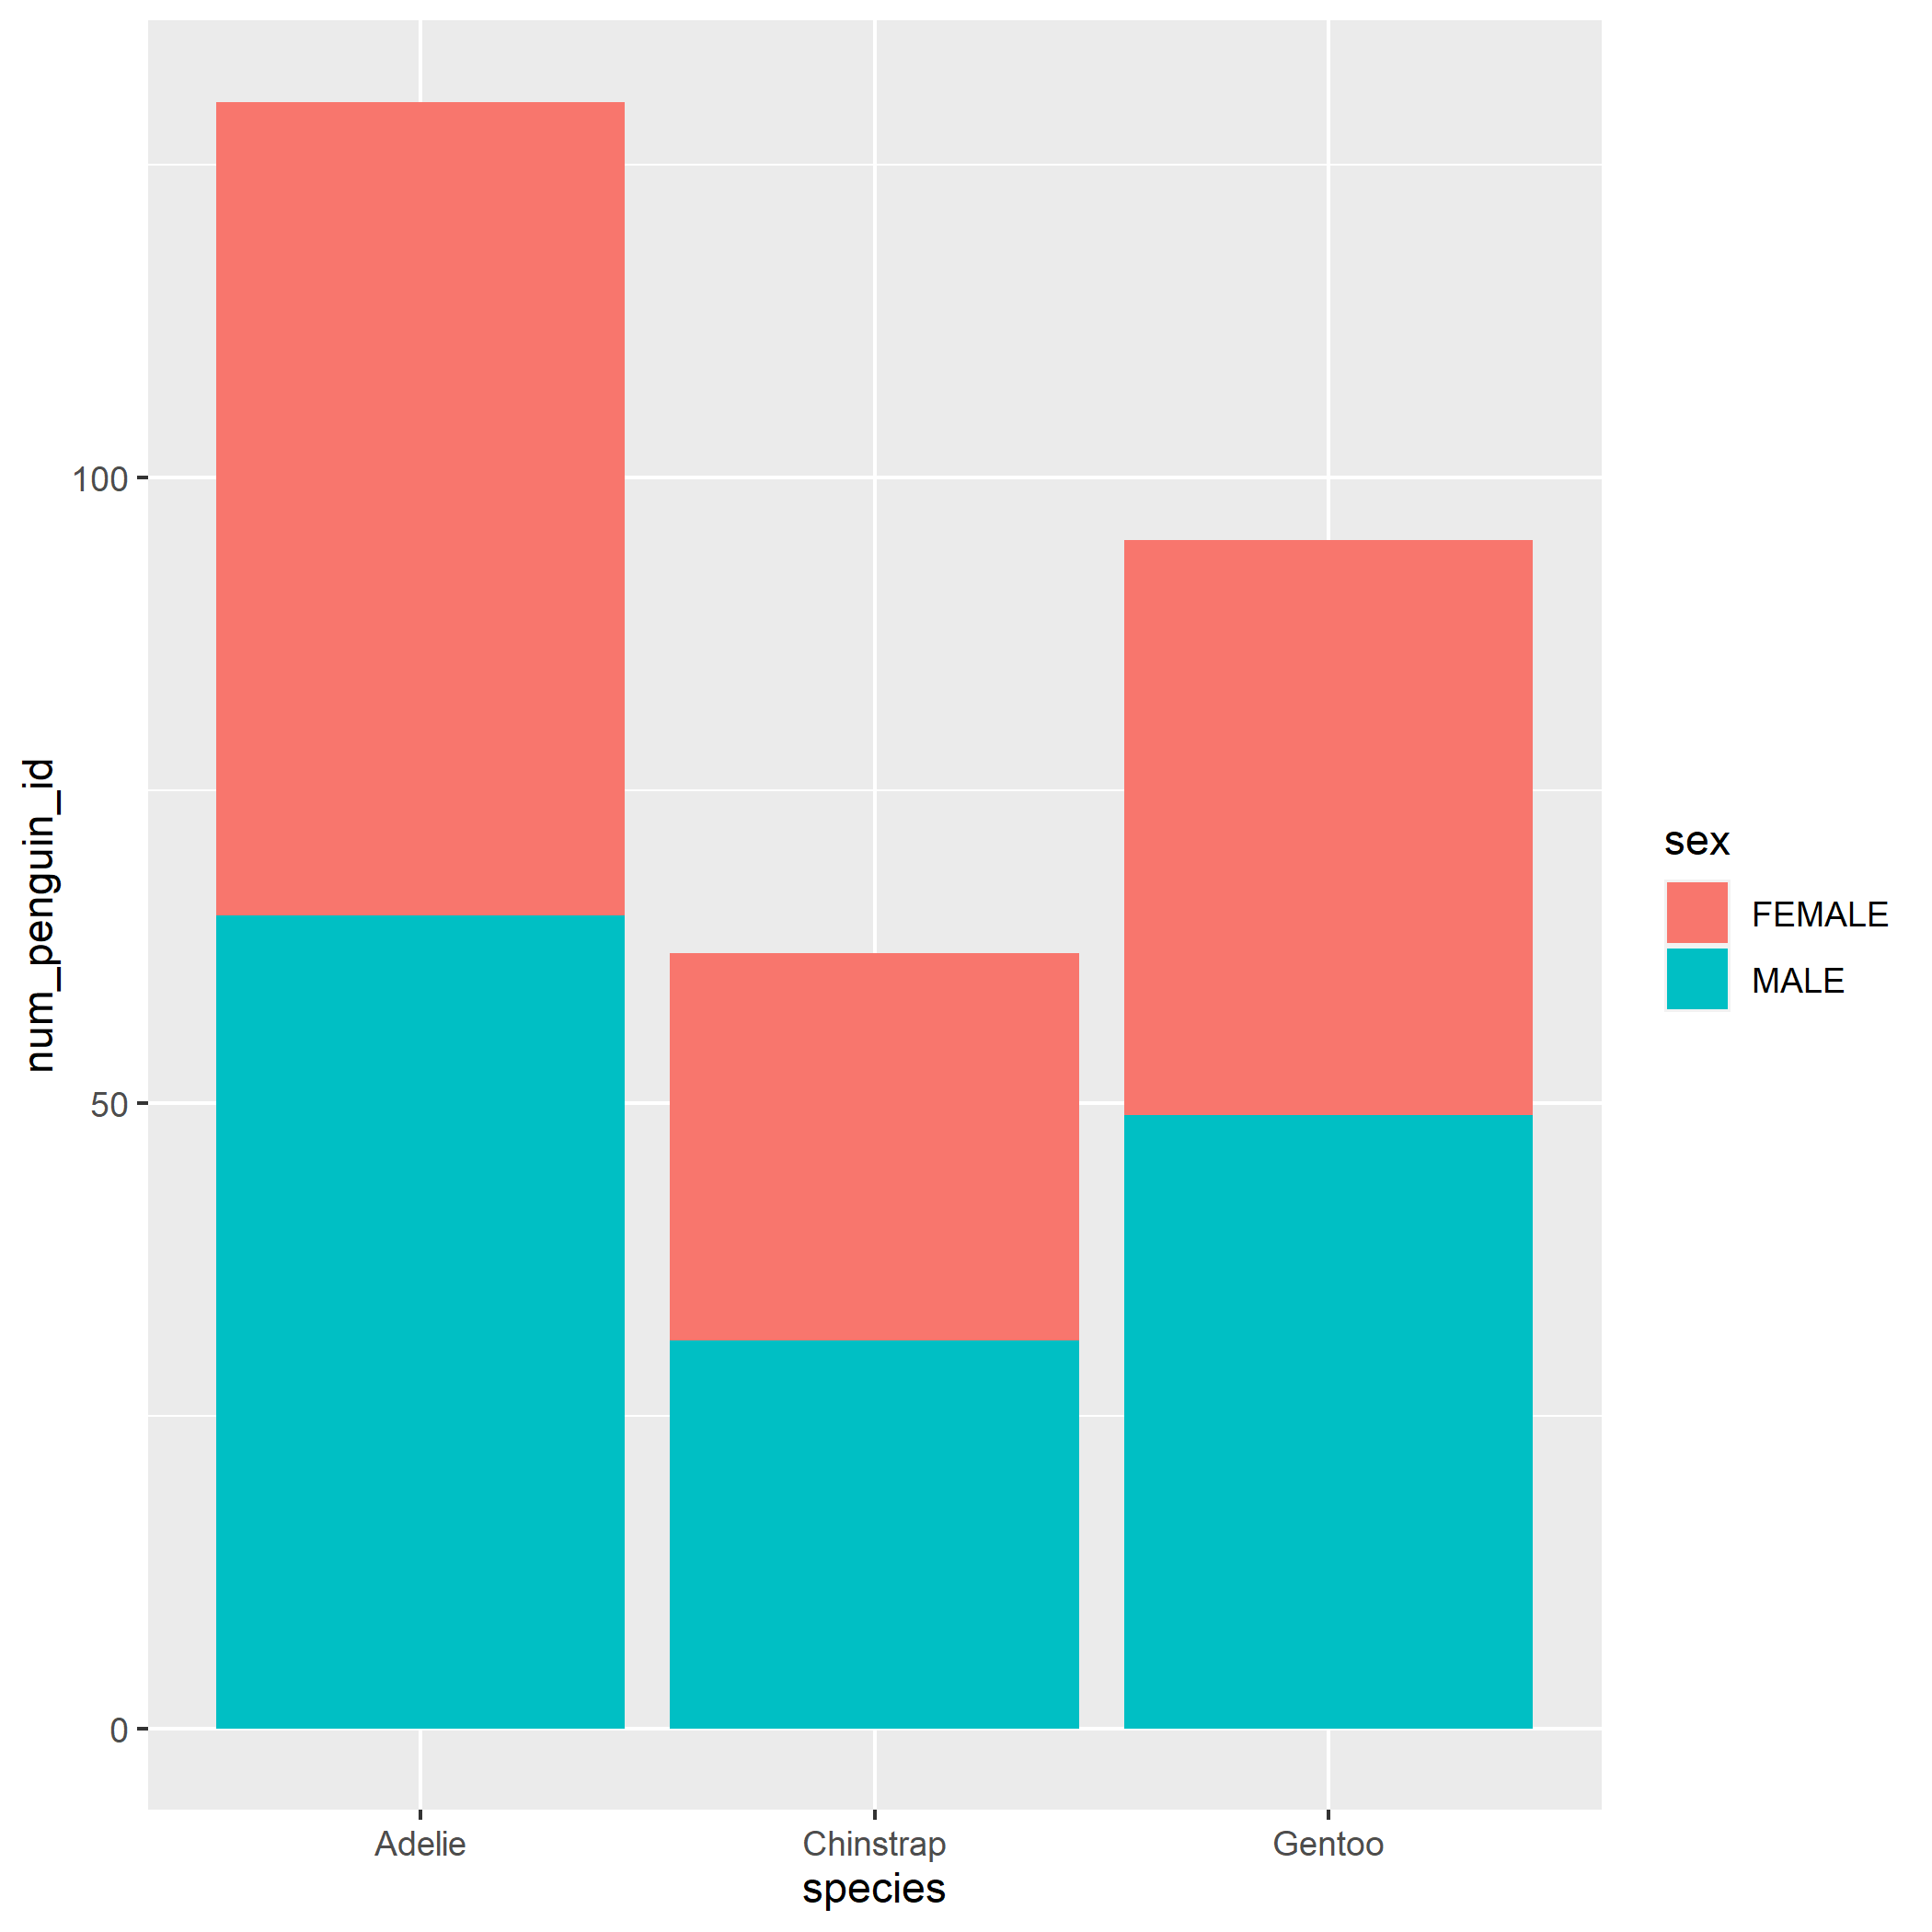
\includegraphics[width=0.8\linewidth]{images/stacked_bar} \caption{A first insight the number of male and female penguins of each species in our study}\label{fig:unnamed-chunk-82}
\end{figure}

We will cover how ggplot works in more detail next week. But in brief, to get the graph we first use the \texttt{ggplot} function, we give \texttt{ggplot} the `aesthetic mappings' of the plot, the values we wish to assign to the x axis, y axis and how we want to ``fill in'' the objects we will draw.

This first line of code will just draw a blank plot, with the \emph{plus} + sign we signify that we want to add a new layer, this builds on top of the first layer and by specifying the function \texttt{geom\_col} we request columns are layered onto the plot. This layer inherits all of the specifications of x,y and fill from \texttt{ggplot()}. And it produces a handy legend.

\hypertarget{challenge}{%
\subsection{Challenge}\label{challenge}}

\begin{rmdquestion}
Can you write and run a script, with appropriate comments, that produces
a summary tibble and graph for the number of penguins of each species,
on the three study islands?
\end{rmdquestion}

\hypertarget{distributions}{%
\section{Distributions}\label{distributions}}

We now know how many penguins were surveyed. Let's move on to look at some distributions. One of our interests was the size of bill lengths, so let's look at the distribution of values in this variable.

Looking at frequency distributions is very \emph{useful} because it shows the shape of the \emph{sample distribution}, that shape is very important for the types of formal statistics we can do later.

Here is the script to plot frequency distribution, as before we pipe the data into ggplot. This time we only specify an x variable because we intend to plot a histogram and the y variable is always the count of observations. We then ask for the data to be presented in 50 equally sized bins of data. So in this case we have chopped the range of the x axis into 50 equal parts and counted the number of observations that fall within each one.

\begin{Shaded}
\begin{Highlighting}[]
\NormalTok{penguins }\SpecialCharTok{\%\textgreater{}\%} 
  \FunctionTok{ggplot}\NormalTok{(}\FunctionTok{aes}\NormalTok{(}\AttributeTok{x=}\NormalTok{culmen\_length\_mm))}\SpecialCharTok{+}
  \FunctionTok{geom\_histogram}\NormalTok{(}\AttributeTok{bins=}\DecValTok{50}\NormalTok{)}
\end{Highlighting}
\end{Shaded}

\begin{figure}
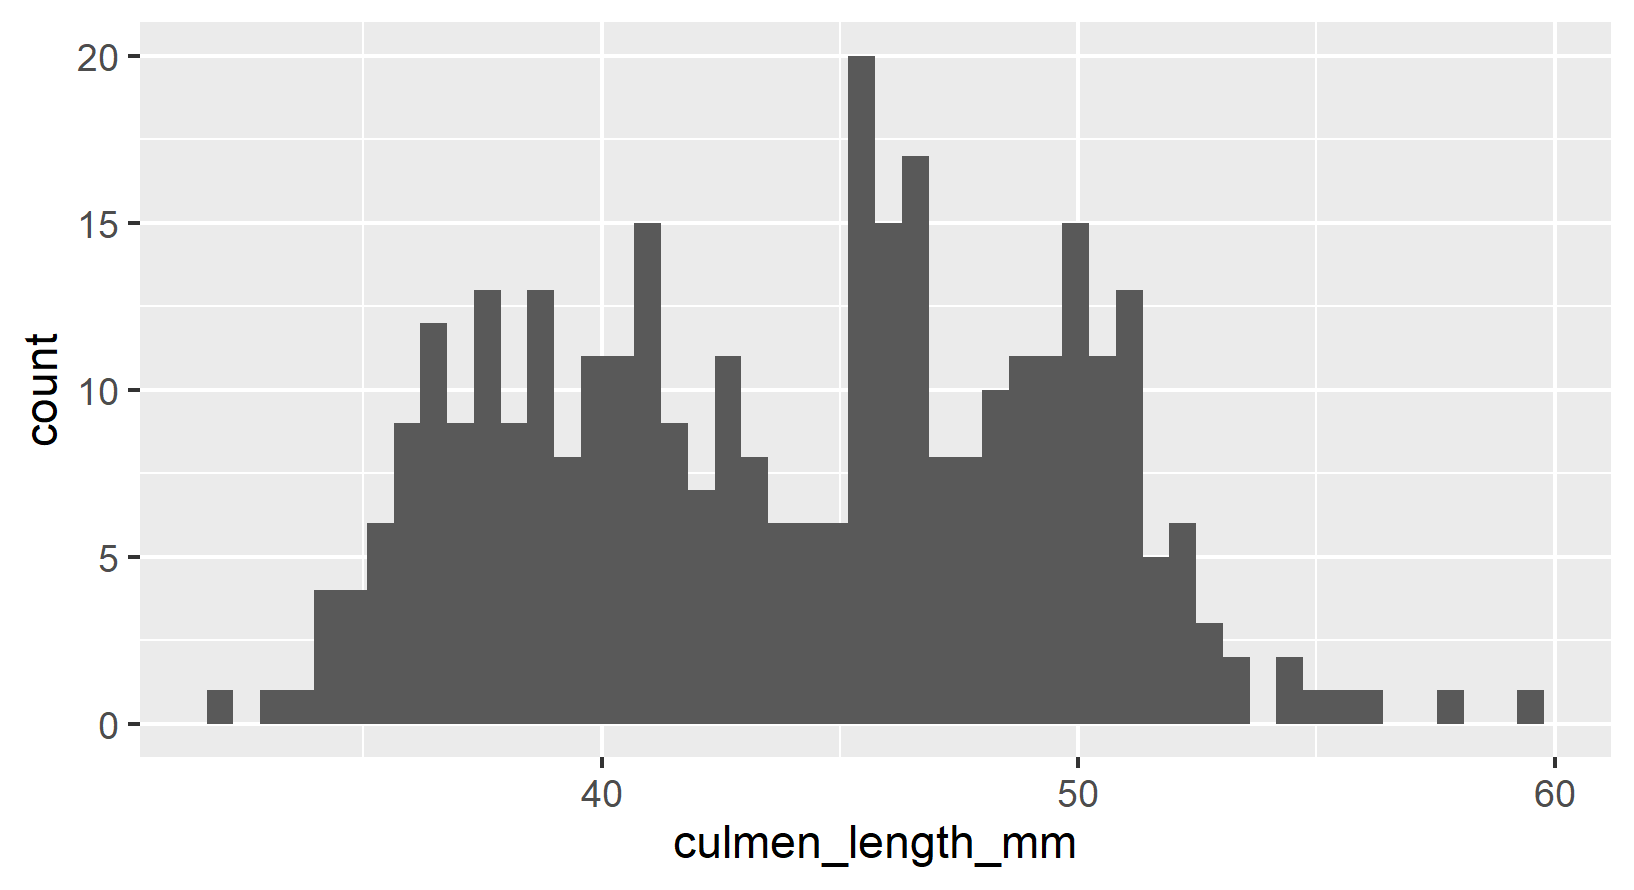
\includegraphics[width=0.8\linewidth]{images/Distribution} \caption{Frequency distribution of culmen length in penguins}\label{fig:unnamed-chunk-85}
\end{figure}

\begin{quote}
** Note - Bins. Have a go at changing the value specified to the bins argument, and observe how the figure changes.
\end{quote}

\hypertarget{insights}{%
\subsection{Insights}\label{insights}}

\begin{rmdquestion}
\begin{itemize}
\item
  Are you surprised at all by the distribution? We have drawn a
  continuous variable from a natural population, what did you expect the
  distribution to look like?
\item
  Can you change the code for the histogram plot to produce
  distributions for each sex?
\item
  How has this changed your interpretation of the distributions?
\end{itemize}
\end{rmdquestion}

\hypertarget{more-distributions}{%
\section{More distributions}\label{more-distributions}}

From the figures you have made, you should be able to make some guesses about the means and medians of the data. But we can use \texttt{dplyr} to get more accurate answers.

\begin{Shaded}
\begin{Highlighting}[]
\CommentTok{\# generate the mean, median and standard deviation of culmen length in three species of penguins}

\NormalTok{penguins }\SpecialCharTok{\%\textgreater{}\%} 
  \FunctionTok{group\_by}\NormalTok{(species) }\SpecialCharTok{\%\textgreater{}\%} 
  \FunctionTok{summarise}\NormalTok{(}\AttributeTok{mean\_culmen\_length=}\FunctionTok{mean}\NormalTok{(culmen\_length\_mm),}
            \AttributeTok{median\_culmen\_length=}\FunctionTok{median}\NormalTok{(culmen\_length\_mm),}
            \AttributeTok{sd\_culmen\_length=}\FunctionTok{sd}\NormalTok{(culmen\_length\_mm))}
\end{Highlighting}
\end{Shaded}

Huh??? What's going on??? We get NAs because there are NAs in our dataset any calculation involving nothing produces nothing. Try this

\begin{Shaded}
\begin{Highlighting}[]
\CommentTok{\# messing about with NA calculations}
\DecValTok{4}\SpecialCharTok{+}\ConstantTok{NA}

\DecValTok{3}\SpecialCharTok{*}\ConstantTok{NA}

\ConstantTok{NA}\SpecialCharTok{\^{}}\DecValTok{2}

\NormalTok{(}\DecValTok{1}\SpecialCharTok{+}\DecValTok{2}\SpecialCharTok{+}\ConstantTok{NA}\NormalTok{)}\SpecialCharTok{/}\DecValTok{2}
\end{Highlighting}
\end{Shaded}

We need to remember to specify the argument to remove \texttt{NA}

\begin{Shaded}
\begin{Highlighting}[]
\CommentTok{\# generate the mean, median and standard deviation of culmen length in three species of penguins}
\CommentTok{\# specify the removal of NA values}
\NormalTok{penguins }\SpecialCharTok{\%\textgreater{}\%} 
  \FunctionTok{group\_by}\NormalTok{(species)}
  \FunctionTok{summarise}\NormalTok{(}\AttributeTok{mean\_culmen\_length=}\FunctionTok{mean}\NormalTok{(culmen\_length\_mm, }\AttributeTok{na.rm=}\ConstantTok{TRUE}\NormalTok{),}
            \AttributeTok{median\_culmen\_length=}\FunctionTok{median}\NormalTok{(culmen\_length\_mm, }\AttributeTok{na.rm=}\ConstantTok{TRUE}\NormalTok{),}
            \AttributeTok{sd\_culmen\_length=}\FunctionTok{sd}\NormalTok{(culmen\_length\_mm, }\AttributeTok{na.rm=}\ConstantTok{TRUE}\NormalTok{))}
\end{Highlighting}
\end{Shaded}

\begin{quote}
The mean and median values for each species are \emph{very} similar, which indicates we do not have much \emph{skew} in our data. This detail is important because statistical analyses make lots of assumptions about the underlying distributions of the data.
\end{quote}

\hypertarget{initial-conclusions}{%
\subsection{Initial conclusions}\label{initial-conclusions}}

In these data we are already able to make some useful insights

\begin{itemize}
\item
  Fewer Chinstrap penguins were surveyed than Adelie or Gentoo's
\item
  The average bill length for Adelie penguins is 38.8 mm, on average 8.7mm shorter than Gentoo's and 10mm shorter than Chinstrap's
\item
  There does not appear to be much difference between Chinstrap and Gentoo bill lengths (on average 1.3mm)
\end{itemize}

These might appear to be modest insights - but have learned several data manipulation and summary techniques. We can also start to take a look at some of our initial hypotheses!!!

\begin{rmdquestion}
\begin{itemize}
\tightlist
\item
  How does this data stack up against the hypothesis about bill
  morphology we put forward last week?
\end{itemize}
\end{rmdquestion}

To make more and conclusive insights we have a bit further to go, but I think you deserve a pat on the back

\begin{Shaded}
\begin{Highlighting}[]
\CommentTok{\# R generate some praise}
\NormalTok{praise}\SpecialCharTok{::}\FunctionTok{praise}\NormalTok{()}
\end{Highlighting}
\end{Shaded}

\hypertarget{data-transformation}{%
\section{Data transformation}\label{data-transformation}}

In the previous section we made some basic insights into observation numbers, distributed by species, sex and location. We also started to gain core insights into some of our central hypotheses, but you have probably noticed we don't actually have a variable on the \texttt{relative\ bill\ lengths/depths}. Why is this important? Well we clearly saw there was a difference in bill lengths between our three species. But we haven't taken into account that some of these species might be very different in body size. Our measure of bill lengths as an indicator of feeding strategy, might be confounded by body size (a bigger penguin is likely to have a bigger bill).

We don't have a variable explicitly called body size. Instead we have to use ``proxies'' suitable proxies might be `flipper length' or `body mass'. Neither is perfect

\begin{itemize}
\tightlist
\item
  Flipper length

  \begin{itemize}
  \tightlist
  \item
    Pros: linked to skeletal structure, constant
  \item
    Cons: relative flipper length could also vary by species
  \end{itemize}
\item
  Body mass

  \begin{itemize}
  \tightlist
  \item
    Pros: more of an indication of central size?
  \item
    Cons: condition dependent, likely to change over the year
  \end{itemize}
\end{itemize}

Let's take a look at the distribution of body mass among our three species.

\begin{Shaded}
\begin{Highlighting}[]
\CommentTok{\# frequency distribution of body mass by species}
\NormalTok{penguins }\SpecialCharTok{\%\textgreater{}\%} 
  \FunctionTok{ggplot}\NormalTok{(}\FunctionTok{aes}\NormalTok{(}\AttributeTok{x=}\NormalTok{body\_mass\_g, }\AttributeTok{fill=}\NormalTok{species))}\SpecialCharTok{+}
  \FunctionTok{geom\_histogram}\NormalTok{(}\AttributeTok{bins=}\DecValTok{50}\NormalTok{)}
\end{Highlighting}
\end{Shaded}

How does the distribution you have found compare with your insights on bill length? We can do this using the \texttt{cor\_test} function from the package \texttt{rstatix} (\citet{R-rstatix}). This package contains a number of `pipe-friendly' simple statistics functions

Add the \texttt{library()} for \texttt{rstatix} at the \textbf{top} of your RScript with an appropriate comment \#

\begin{Shaded}
\begin{Highlighting}[]
\CommentTok{\# a simple correlation test from the rstatix package}
\NormalTok{penguins }\SpecialCharTok{\%\textgreater{}\%} 
  \FunctionTok{group\_by}\NormalTok{(species) }\SpecialCharTok{\%\textgreater{}\%} \CommentTok{\# group by species}
  \FunctionTok{cor\_test}\NormalTok{(body\_mass\_g, culmen\_length\_mm) }\CommentTok{\# correlation between body mass and bill length}
\end{Highlighting}
\end{Shaded}

We can see that these two variables `co-vary' a lot, but this appears to be quite species specific. We can already make the insight that Chinstrap penguins appear to have the shortest bill length relative to body mass.

We can make a new variable that is the `relative size of culmen length compared to flipper length'

\begin{Shaded}
\begin{Highlighting}[]
\CommentTok{\# use mutate to produce a new variable that is a ratio of culmen length to flipper length}
\NormalTok{penguins }\OtherTok{\textless{}{-}}\NormalTok{ penguins }\SpecialCharTok{\%\textgreater{}\%} 
  \FunctionTok{mutate}\NormalTok{(}\AttributeTok{relative\_bill\_length =}\NormalTok{ culmen\_length\_mm}\SpecialCharTok{/}\NormalTok{body\_mass\_g)}
\end{Highlighting}
\end{Shaded}

We are probably also interested in bill depth?

\begin{Shaded}
\begin{Highlighting}[]
\CommentTok{\# use mutate to produce a new variable that is a ratio of culmen depth to flipper length}
\NormalTok{penguins }\OtherTok{\textless{}{-}}\NormalTok{ penguins }\SpecialCharTok{\%\textgreater{}\%} 
  \FunctionTok{mutate}\NormalTok{(}\AttributeTok{relative\_bill\_depth =}\NormalTok{ culmen\_depth\_mm}\SpecialCharTok{/}\NormalTok{body\_mass\_g)}

\CommentTok{\# check that these new variables have been included in the dataset}
\NormalTok{penguins }\SpecialCharTok{\%\textgreater{}\%} 
  \FunctionTok{names}\NormalTok{()}
\end{Highlighting}
\end{Shaded}

\hypertarget{developing-insights}{%
\section{Developing insights}\label{developing-insights}}

First let's focus on the distributions of four variables of interest. Then we will progress on to look at their relationships and differences

\begin{itemize}
\item
  relative\_bill\_length
\item
  relative\_bill\_depth
\item
  delta\_15n
\item
  delta\_13c
\end{itemize}

\hypertarget{distributions-of-the-relative-bill-length}{%
\subsection{Distributions of the relative bill length}\label{distributions-of-the-relative-bill-length}}

We will examine the shape of the \emph{sample distribution} of the data again by using histograms.

\begin{Shaded}
\begin{Highlighting}[]
\CommentTok{\# frequency distribution of relative bill length by species}
\CommentTok{\# we already know we are interested in looking at the distributions \textquotesingle{}within\textquotesingle{} each species}
\NormalTok{penguins }\SpecialCharTok{\%\textgreater{}\%} 
  \FunctionTok{ggplot}\NormalTok{(}\FunctionTok{aes}\NormalTok{(}\AttributeTok{x=}\NormalTok{relative\_bill\_length, }\AttributeTok{fill=}\NormalTok{species))}\SpecialCharTok{+}
  \FunctionTok{geom\_histogram}\NormalTok{(}\AttributeTok{bins=}\DecValTok{50}\NormalTok{)}
\end{Highlighting}
\end{Shaded}

\begin{figure}
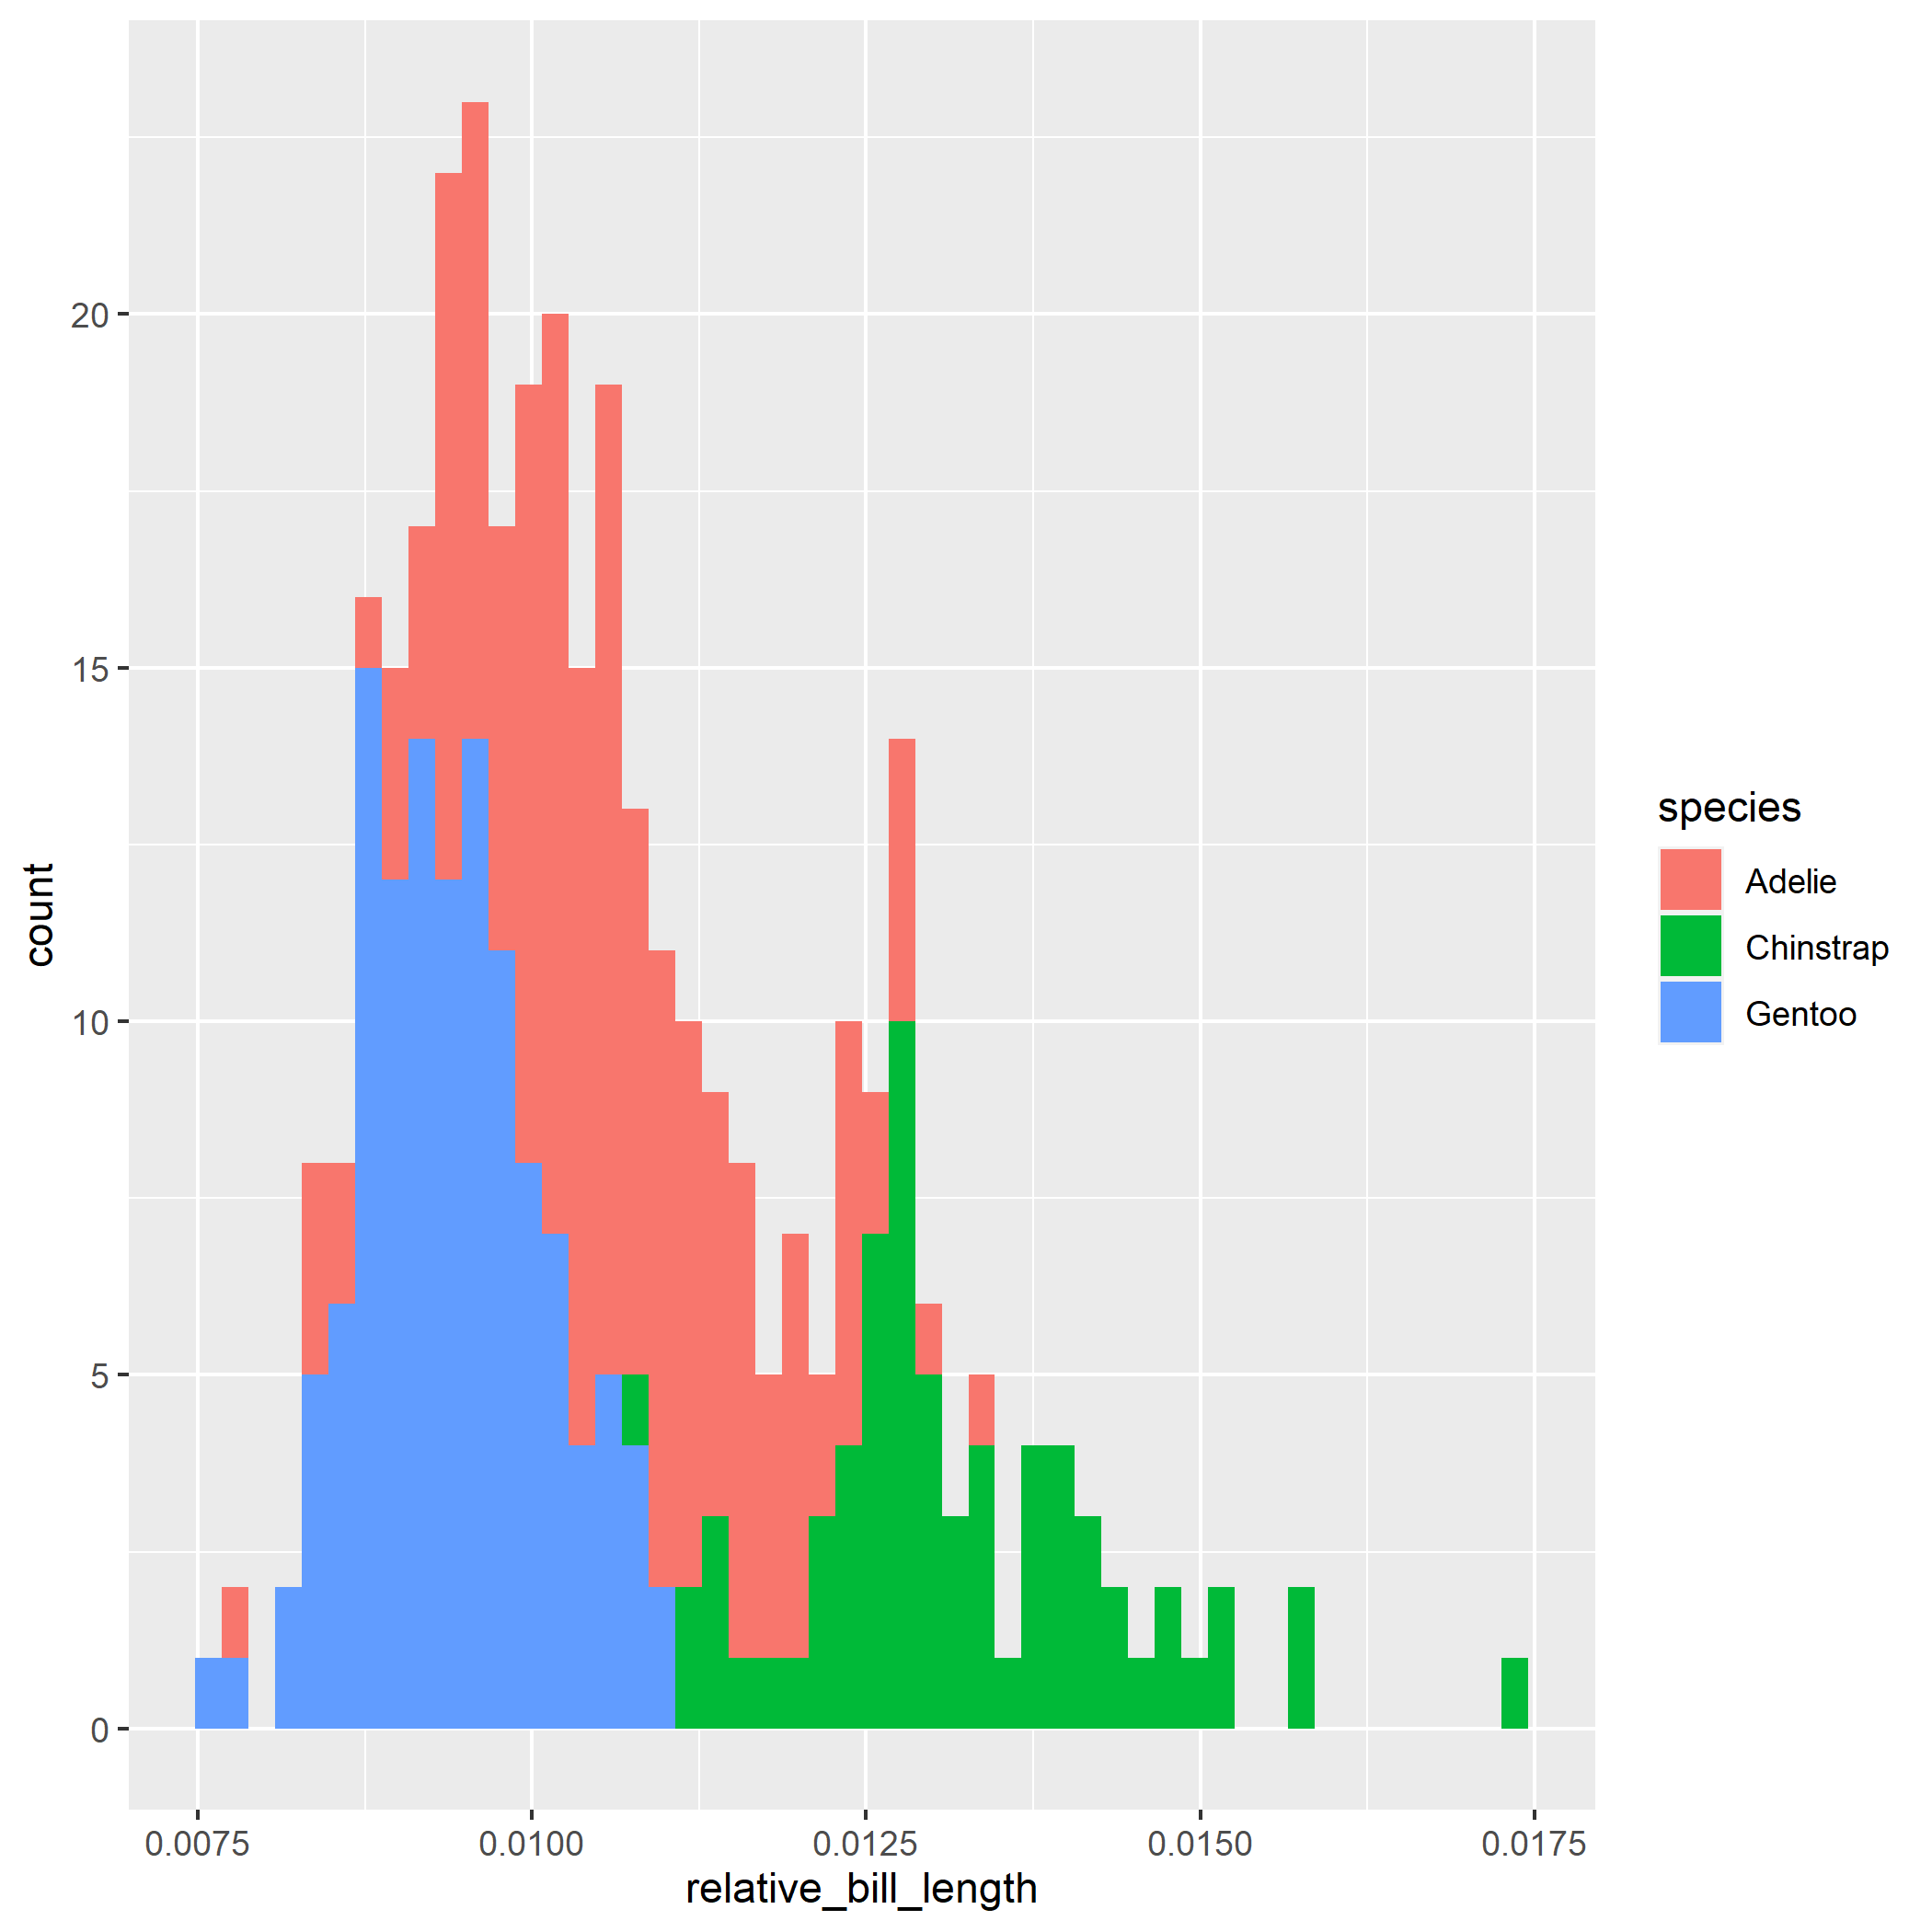
\includegraphics[width=0.8\linewidth]{images/bill_length_distribution} \caption{Frequency distribution of relative bill length in three species of penguins, Adelie, Chinstrap and Gentoo}\label{fig:unnamed-chunk-97}
\end{figure}

Important questions, what shape is the distribution?

\begin{itemize}
\item
  First there must be a lower limit of zero (penguins cannot have negative length bills), does this lead to any truncating of the expected normal distribution bell curve? It doesn't look it.
\item
  Is it symmetrical? Mostly.
\end{itemize}

If it's a little difficult to see - we can separate out these figures using the handy function \texttt{facet\_wrap}

\begin{Shaded}
\begin{Highlighting}[]
\CommentTok{\# frequency distribution of relative bill length by species}
\CommentTok{\# we already know we are interested in looking at the distributions \textquotesingle{}within\textquotesingle{} each species}
\NormalTok{penguins }\SpecialCharTok{\%\textgreater{}\%} 
  \FunctionTok{ggplot}\NormalTok{(}\FunctionTok{aes}\NormalTok{(}\AttributeTok{x=}\NormalTok{relative\_bill\_length, }\AttributeTok{fill=}\NormalTok{species))}\SpecialCharTok{+}
  \FunctionTok{geom\_histogram}\NormalTok{(}\AttributeTok{bins=}\DecValTok{50}\NormalTok{)}\SpecialCharTok{+}
  \FunctionTok{facet\_wrap}\NormalTok{(}\SpecialCharTok{\textasciitilde{}}\NormalTok{species) }\CommentTok{\# facet wrap to look at the separate species more easily}
\end{Highlighting}
\end{Shaded}

\textbackslash begin\{figure\}
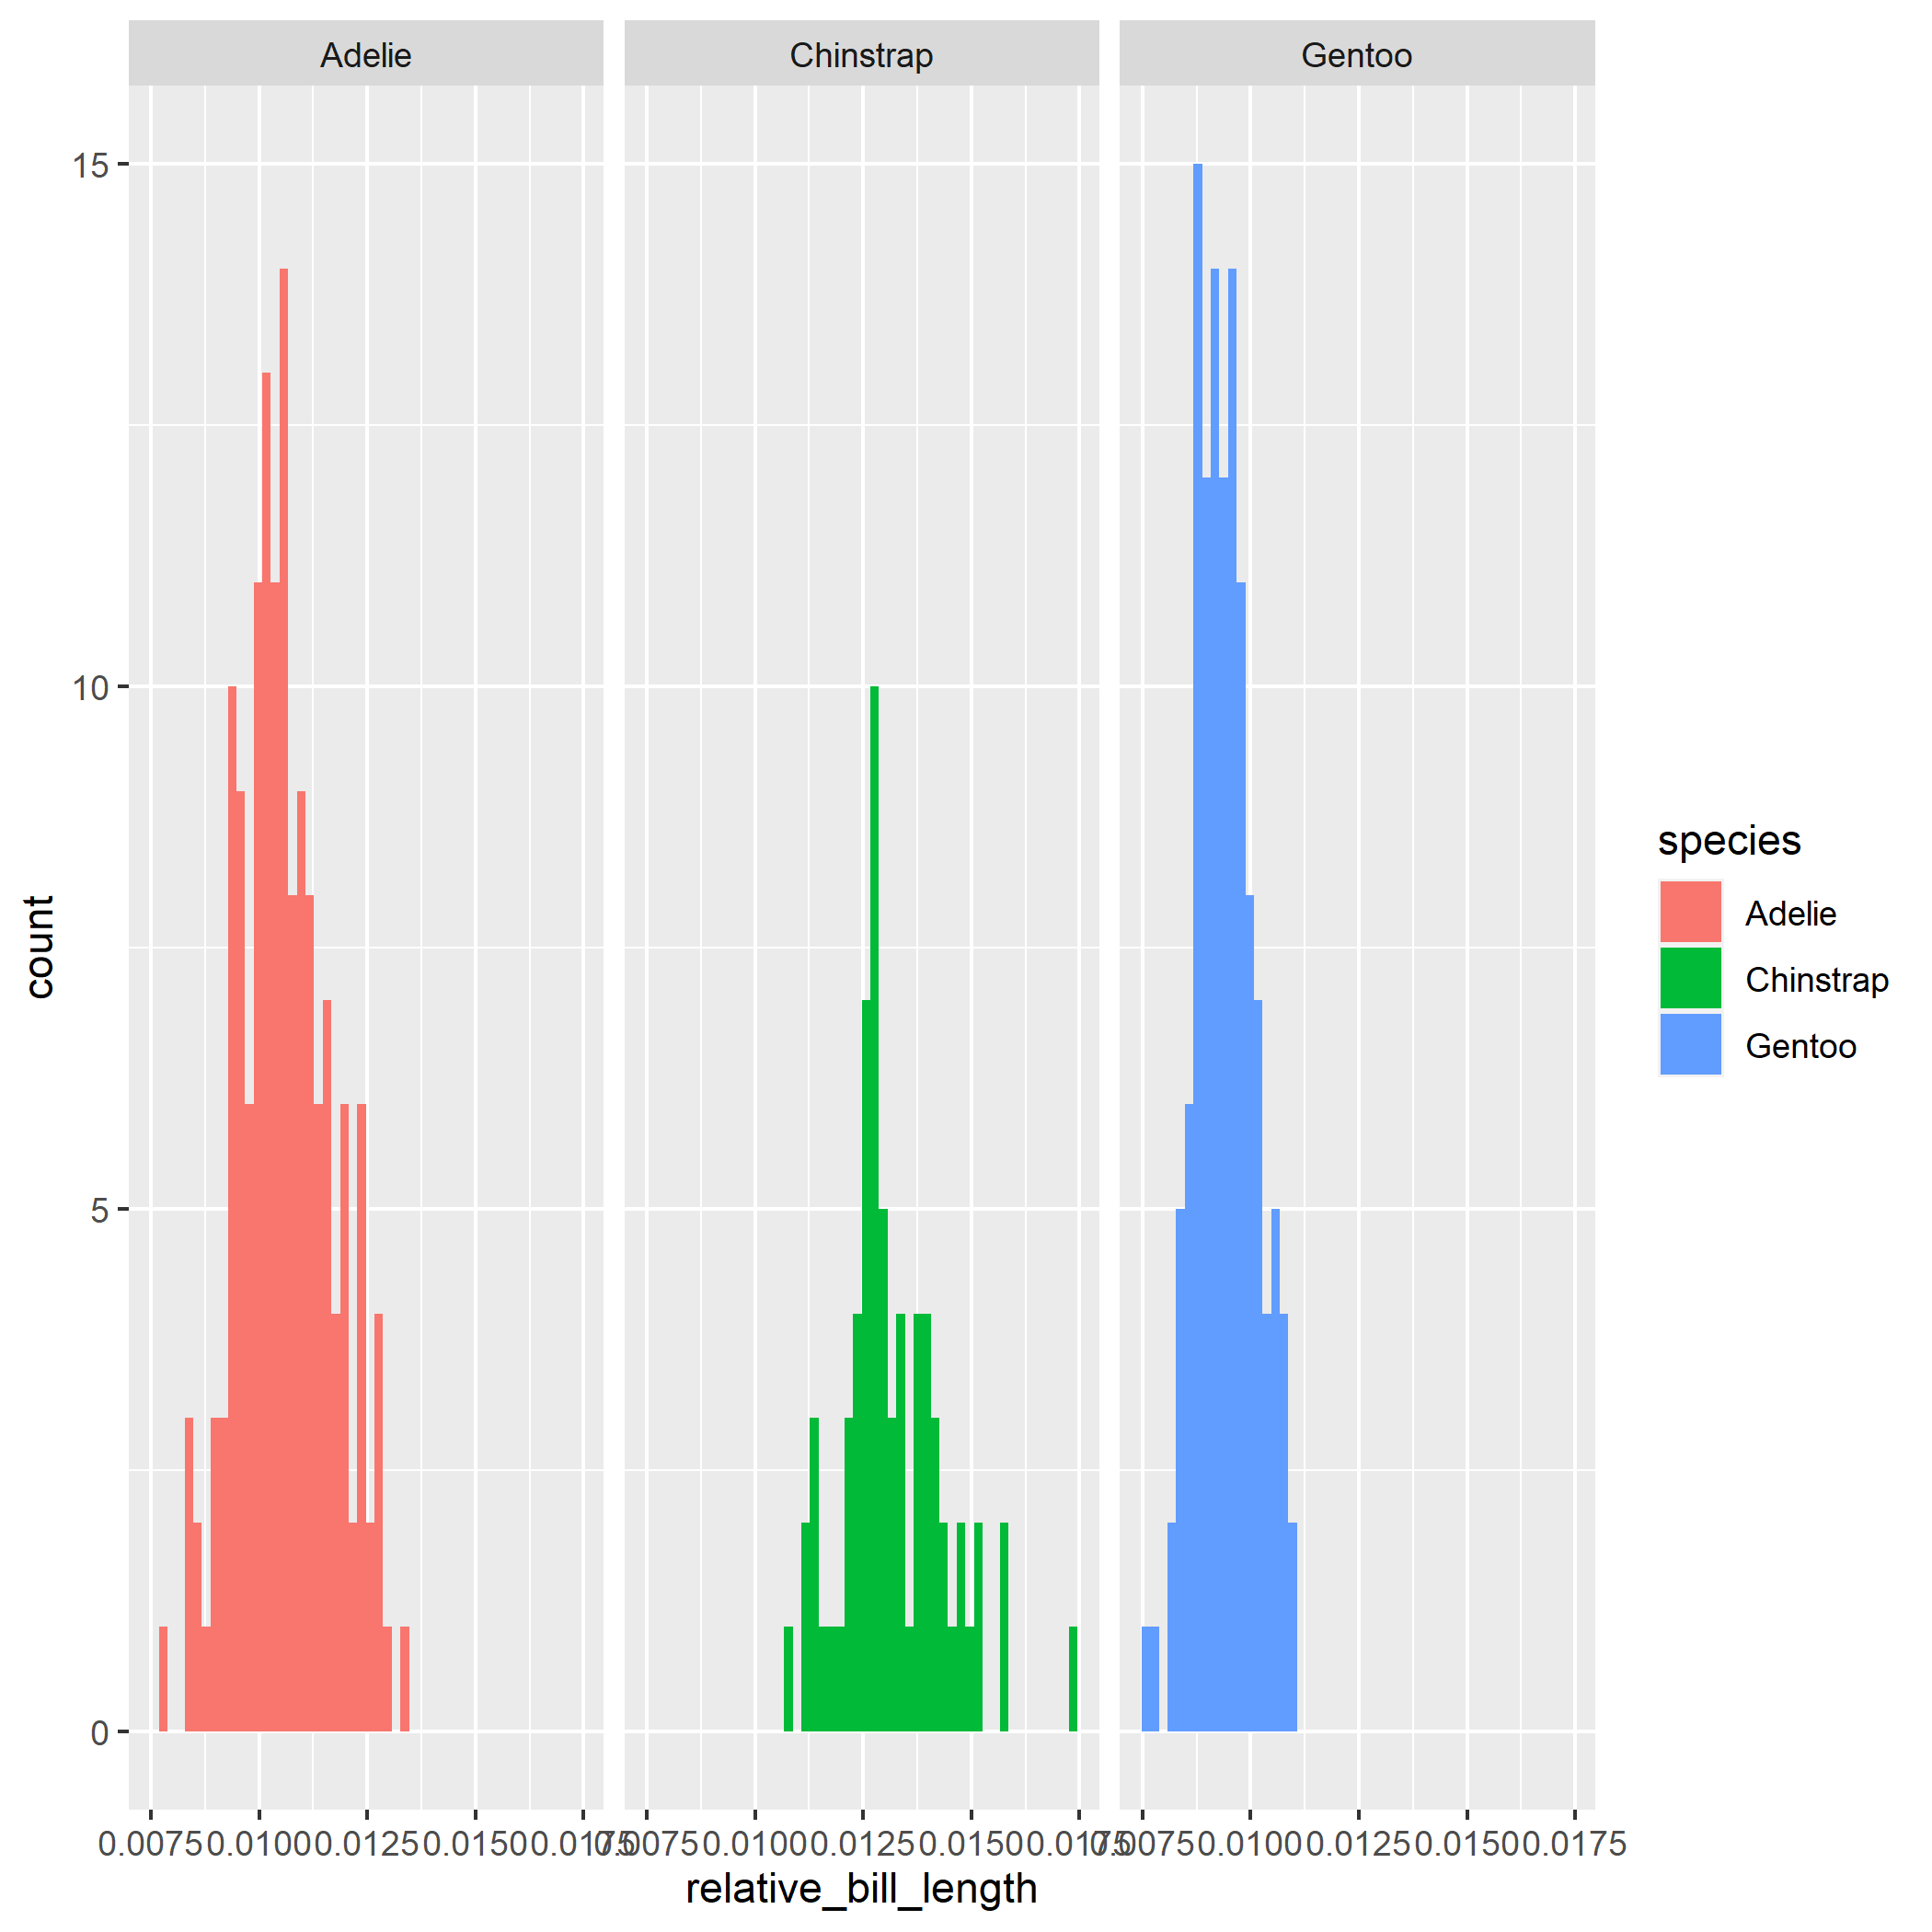
\includegraphics[width=1\linewidth]{images/facetdistribution} \textbackslash caption\{Frequency distribution of relative bill length in three species of penguins, Adelie, Chinstrap and Gentoo - histograms split into three panes by facet\_wrap\}\label{fig:unnamed-chunk-99}
\textbackslash end\{figure\}

\begin{rmdquestion}
Looking at these distributions, how do you think the mean \& median
values will compare in these three species? Think about it first - then
run the code below.
\end{rmdquestion}

\begin{Shaded}
\begin{Highlighting}[]
\CommentTok{\# Mean and Median summaries}
\NormalTok{penguins }\SpecialCharTok{\%\textgreater{}\%} 
  \FunctionTok{group\_by}\NormalTok{(species) }\SpecialCharTok{\%\textgreater{}\%} 
  \FunctionTok{summarise}\NormalTok{(}\AttributeTok{mean\_relative\_bill\_length=}\FunctionTok{mean}\NormalTok{(relative\_bill\_length, }\AttributeTok{na.rm=}\ConstantTok{TRUE}\NormalTok{),}
            \AttributeTok{median\_relative\_bill\_length=}\FunctionTok{median}\NormalTok{(relative\_bill\_length, }\AttributeTok{na.rm=}\ConstantTok{TRUE}\NormalTok{))}
\end{Highlighting}
\end{Shaded}

\begin{verbatim}
# A tibble: 3 x 3
  species   mean_relative_bill_length median_relative_bill_length
  <chr>                         <dbl>                       <dbl>
1 Adelie                      0.0106                      0.0105 
2 Chinstrap                   0.0132                      0.0129 
3 Gentoo                      0.00941                     0.00939
\end{verbatim}

We can see that the mean and median values are almost identical for each species. This indicates we \emph{aren't} dealing with a lot of skew, this is important for when using statistics, which are based on a lot of assumptions like normal distribution.

\begin{rmdquestion}
Can you \textbf{repeat} these steps for the variable
\texttt{relative\_bill\_depth}, \texttt{delta\_15n} and
\texttt{delta\_13c} - add all appropriate comments and commands to your
R Script.
\end{rmdquestion}

\hypertarget{relationshipdifferences}{%
\section{Relationship/differences}\label{relationshipdifferences}}

Getting proper data insights involves looking for relationships or differences.
Remember, if we have a manipulated variable in a well-designed experiment, we may be able to identify a causal effect. With a study without this manipulation, like this penguin study - we cannot be sure any relationships or differences are causal. We have to include some caution in our interpretations.

\hypertarget{differences}{%
\subsection{Differences}\label{differences}}

We have already looked at frequency distributions of the data, where it is possible to see differences. However we can use ggplot and \texttt{geom\_point} to produce difference plots.

\begin{Shaded}
\begin{Highlighting}[]
\CommentTok{\# specifying position with a jitter argument positions points randomly across the x axis this prevents overcrowding}
\NormalTok{penguins }\SpecialCharTok{\%\textgreater{}\%} 
    \FunctionTok{ggplot}\NormalTok{(}\FunctionTok{aes}\NormalTok{(}\AttributeTok{x=}\NormalTok{species, }
               \AttributeTok{y=}\NormalTok{culmen\_length\_mm, }
               \AttributeTok{colour=}\NormalTok{species))}\SpecialCharTok{+} \CommentTok{\# some geoms use color rather than fill to specify colour}
    \FunctionTok{geom\_point}\NormalTok{(}\AttributeTok{position=}\FunctionTok{position\_jitter}\NormalTok{(}\AttributeTok{width=}\FloatTok{0.2}\NormalTok{)) }
\end{Highlighting}
\end{Shaded}

\begin{figure}
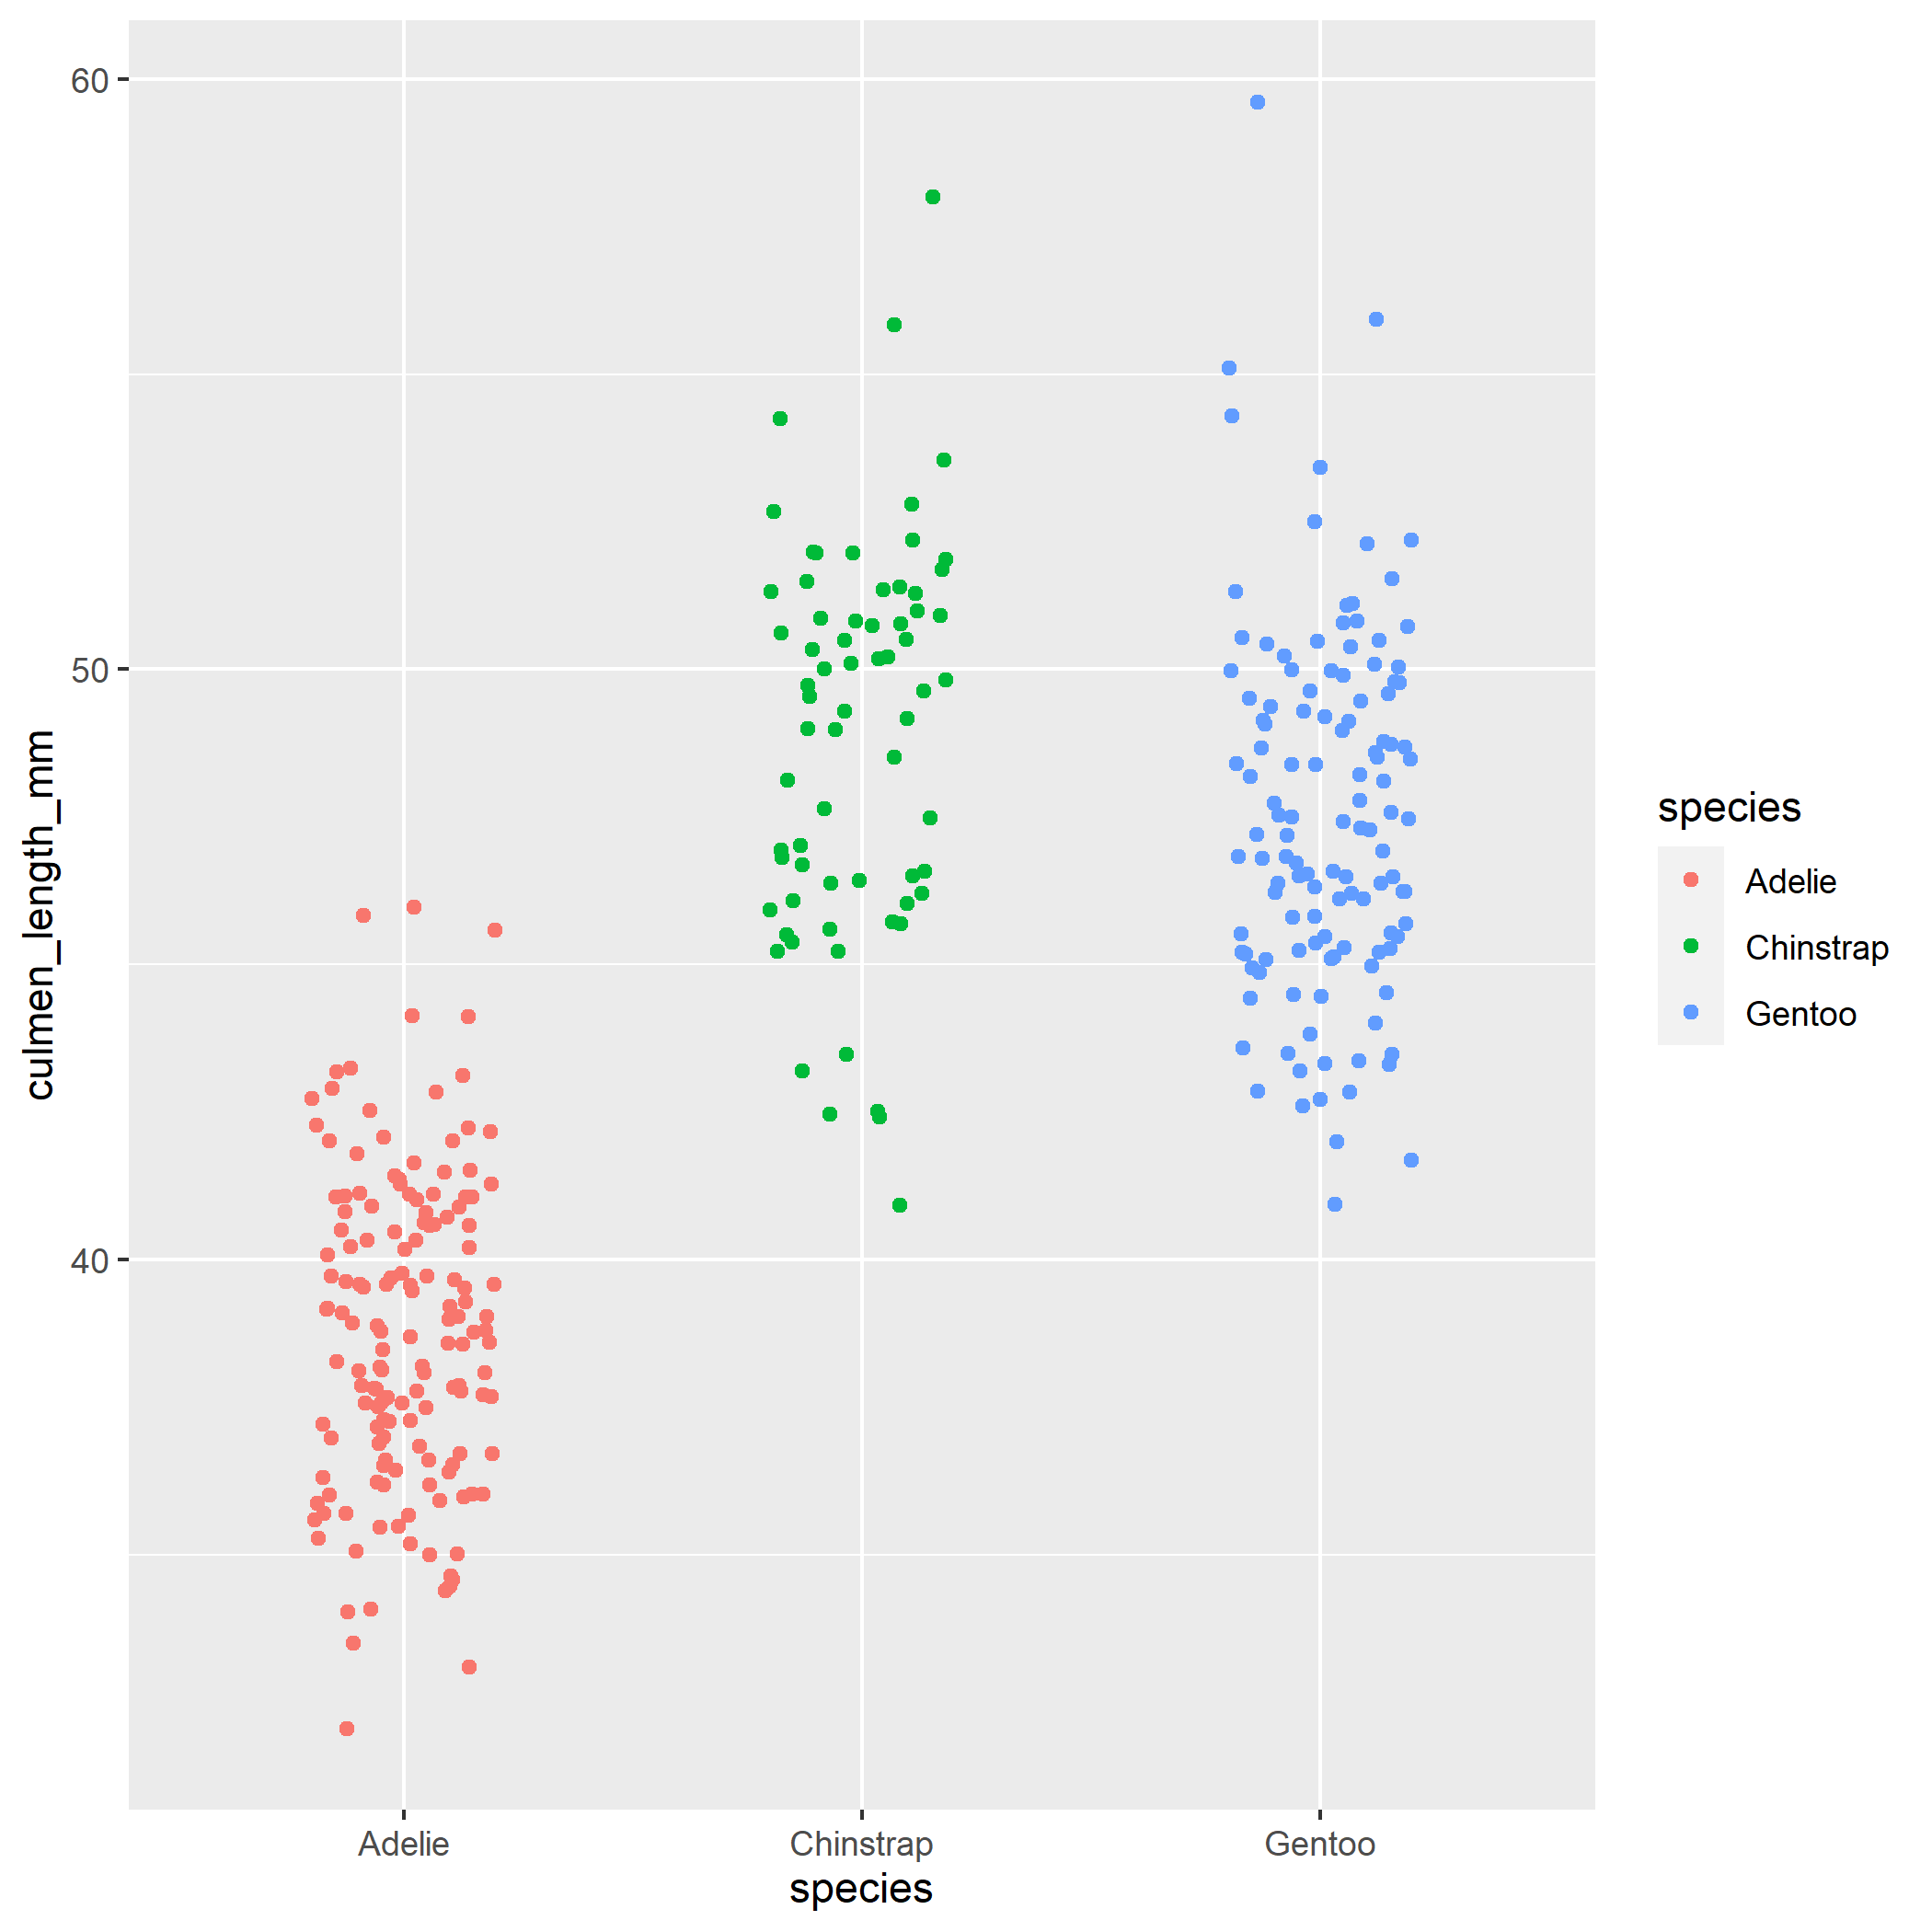
\includegraphics[width=1\linewidth]{images/jitterplot} \caption{Differences in relative bill length of three different species of Antarctic Penguin.}\label{fig:unnamed-chunk-104}
\end{figure}

\begin{quote}
**Note - try altering the width argument and see how it affects the output of the plot.
We will do a deeper dive into ggplot later.
\end{quote}

\begin{rmdquestion}
Try producing these figures for the \texttt{culmen\_depth\_mm},
\texttt{delta\_15n} and \texttt{delta\_13c} variables as well.

What are you observations of the relative differences?
\end{rmdquestion}

\hypertarget{associations}{%
\subsection{Associations}\label{associations}}

It might also be of interest to look at whether any of our variables of interest are strongly associated. For example what is the relationship between heavy carbon/heavy nitrogen isotopes?

\begin{Shaded}
\begin{Highlighting}[]
\NormalTok{penguins }\SpecialCharTok{\%\textgreater{}\%} 
    \FunctionTok{ggplot}\NormalTok{(}\FunctionTok{aes}\NormalTok{(}\AttributeTok{x=}\NormalTok{delta\_15n, }\AttributeTok{y=}\NormalTok{delta\_13c, }\AttributeTok{colour=}\NormalTok{species))}\SpecialCharTok{+}
    \FunctionTok{geom\_point}\NormalTok{()}\SpecialCharTok{+}
    \FunctionTok{geom\_smooth}\NormalTok{(}\AttributeTok{method=}\StringTok{"lm"}\NormalTok{, }\CommentTok{\# produces a simple regression line}
                \AttributeTok{se=}\ConstantTok{FALSE}\NormalTok{)    }\CommentTok{\# no standard error intervals}
\end{Highlighting}
\end{Shaded}

\begin{figure}
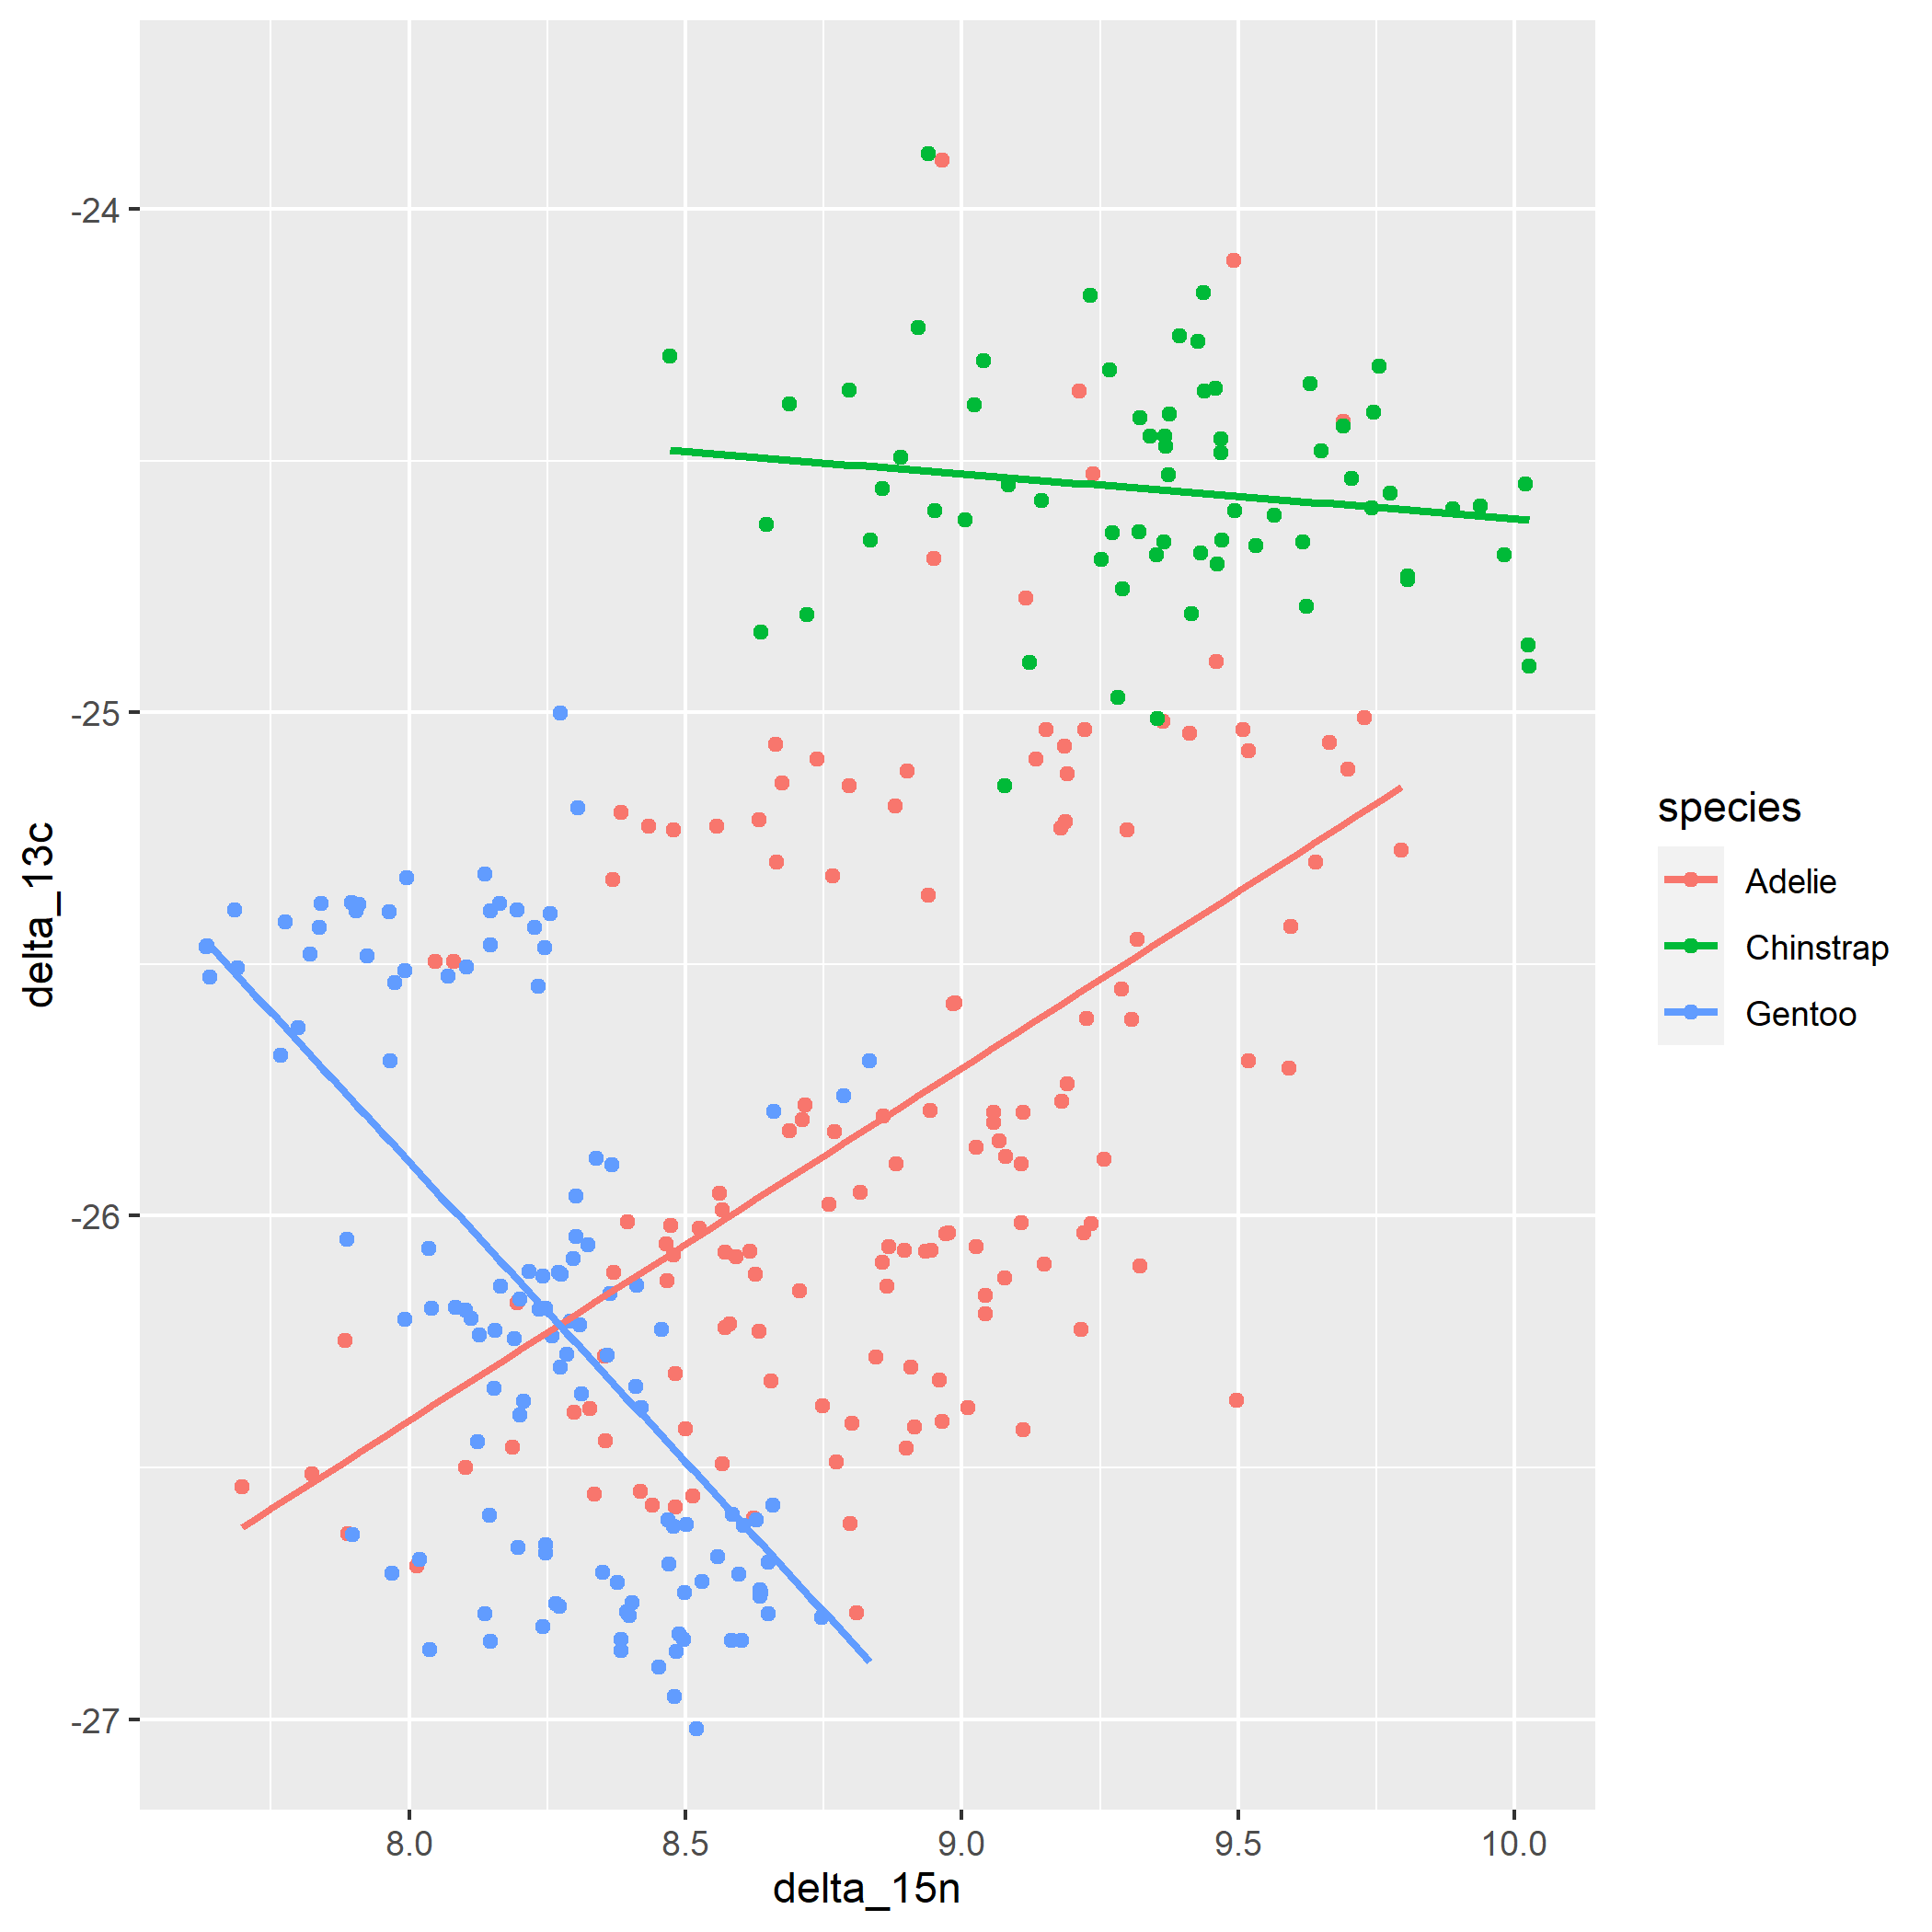
\includegraphics[width=1\linewidth]{images/corrplot} \caption{Asssocation between heavy Nitrogen and heavy Carbon isotopes in blood samples from three Antarctic Penguin species}\label{fig:unnamed-chunk-107}
\end{figure}

We can see here that the association between these isotopes varies a lot by different species, there is probably quite a complex relationship here. It also indicates we should probably investigate these two isotopes separately.

\begin{itemize}
\tightlist
\item
  Have a look at the relative bill length and depth relationships as well
\end{itemize}

\hypertarget{sex-interactions}{%
\section{Sex interactions}\label{sex-interactions}}

Now let's concern ourselves with interactions. We have \emph{already} seen how our interpretation of certain variables can be heavily altered if we don't take into account important contexts - like morphology in relation to species.

Thinking about sensible interactions takes patience and good biological understanding, the payoff is it can produce unique insights.

Focusing on relative bill length, we have seen there are differences between species, however we have not considered the potential association of sex. In many species males and females are `dimorphic' and this has the potential to influence our observations if:

\begin{itemize}
\item
  sex has a substantial/bigger effect on morphology than species
\item
  uneven numbers of males/females were scored in our studies
\end{itemize}

Using \texttt{summarise} \texttt{group\_by} and \texttt{n\_distinct} you should quickly be able to check the numbers of males and females surveyed within each species.

\begin{verbatim}
# A tibble: 6 x 3
# Groups:   species [3]
  species   sex    num_penguin_id
  <chr>     <chr>           <int>
1 Adelie    FEMALE             65
2 Adelie    MALE               65
3 Chinstrap FEMALE             31
4 Chinstrap MALE               31
5 Gentoo    FEMALE             46
6 Gentoo    MALE               49
\end{verbatim}

Looks like numbers are even, which is good. Again focusing on relative bill length let's generate some figures breaking down this variable by sex and species.

First let's generate some more simple summary stats - this time we are assigning it to an object to use later

\begin{Shaded}
\begin{Highlighting}[]
\NormalTok{penguin\_stats }\OtherTok{\textless{}{-}}\NormalTok{ penguins }\SpecialCharTok{\%\textgreater{}\%} 
  \FunctionTok{group\_by}\NormalTok{(sex, species) }\SpecialCharTok{\%\textgreater{}\%} 
  \FunctionTok{summarise}\NormalTok{(}\AttributeTok{mean\_relative\_bill\_length=}\FunctionTok{mean}\NormalTok{(relative\_bill\_length, }\AttributeTok{na.rm=}\ConstantTok{TRUE}\NormalTok{))}
\end{Highlighting}
\end{Shaded}

Now we are going to make our first figure which includes both raw and summary data. Copy and run the code below, and see if you can add comments next to the arguments you are unfamiliar with about what they might be doing.

\begin{Shaded}
\begin{Highlighting}[]
\NormalTok{penguins }\SpecialCharTok{\%\textgreater{}\%} 
  \FunctionTok{drop\_na}\NormalTok{(sex) }\SpecialCharTok{\%\textgreater{}\%} 
  \FunctionTok{ggplot}\NormalTok{(}\FunctionTok{aes}\NormalTok{(}\AttributeTok{x=}\NormalTok{sex, }
             \AttributeTok{y=}\NormalTok{relative\_bill\_length))}\SpecialCharTok{+}
  \FunctionTok{geom\_jitter}\NormalTok{(}\AttributeTok{position=}\FunctionTok{position\_jitter}\NormalTok{(}\AttributeTok{width=}\FloatTok{0.2}\NormalTok{), }
              \AttributeTok{alpha=}\FloatTok{0.4}\NormalTok{)}\SpecialCharTok{+}
  \FunctionTok{geom\_point}\NormalTok{(}\AttributeTok{data=}\NormalTok{penguin\_stats, }\FunctionTok{aes}\NormalTok{(}\AttributeTok{x=}\NormalTok{sex, }
                                     \AttributeTok{y=}\NormalTok{mean\_relative\_bill\_length), }
             \AttributeTok{size=}\DecValTok{4}\NormalTok{, }
             \AttributeTok{color=}\StringTok{"blue"}\NormalTok{)}\SpecialCharTok{+}
  \FunctionTok{facet\_wrap}\NormalTok{(}\SpecialCharTok{\textasciitilde{}}\NormalTok{species)}
\end{Highlighting}
\end{Shaded}

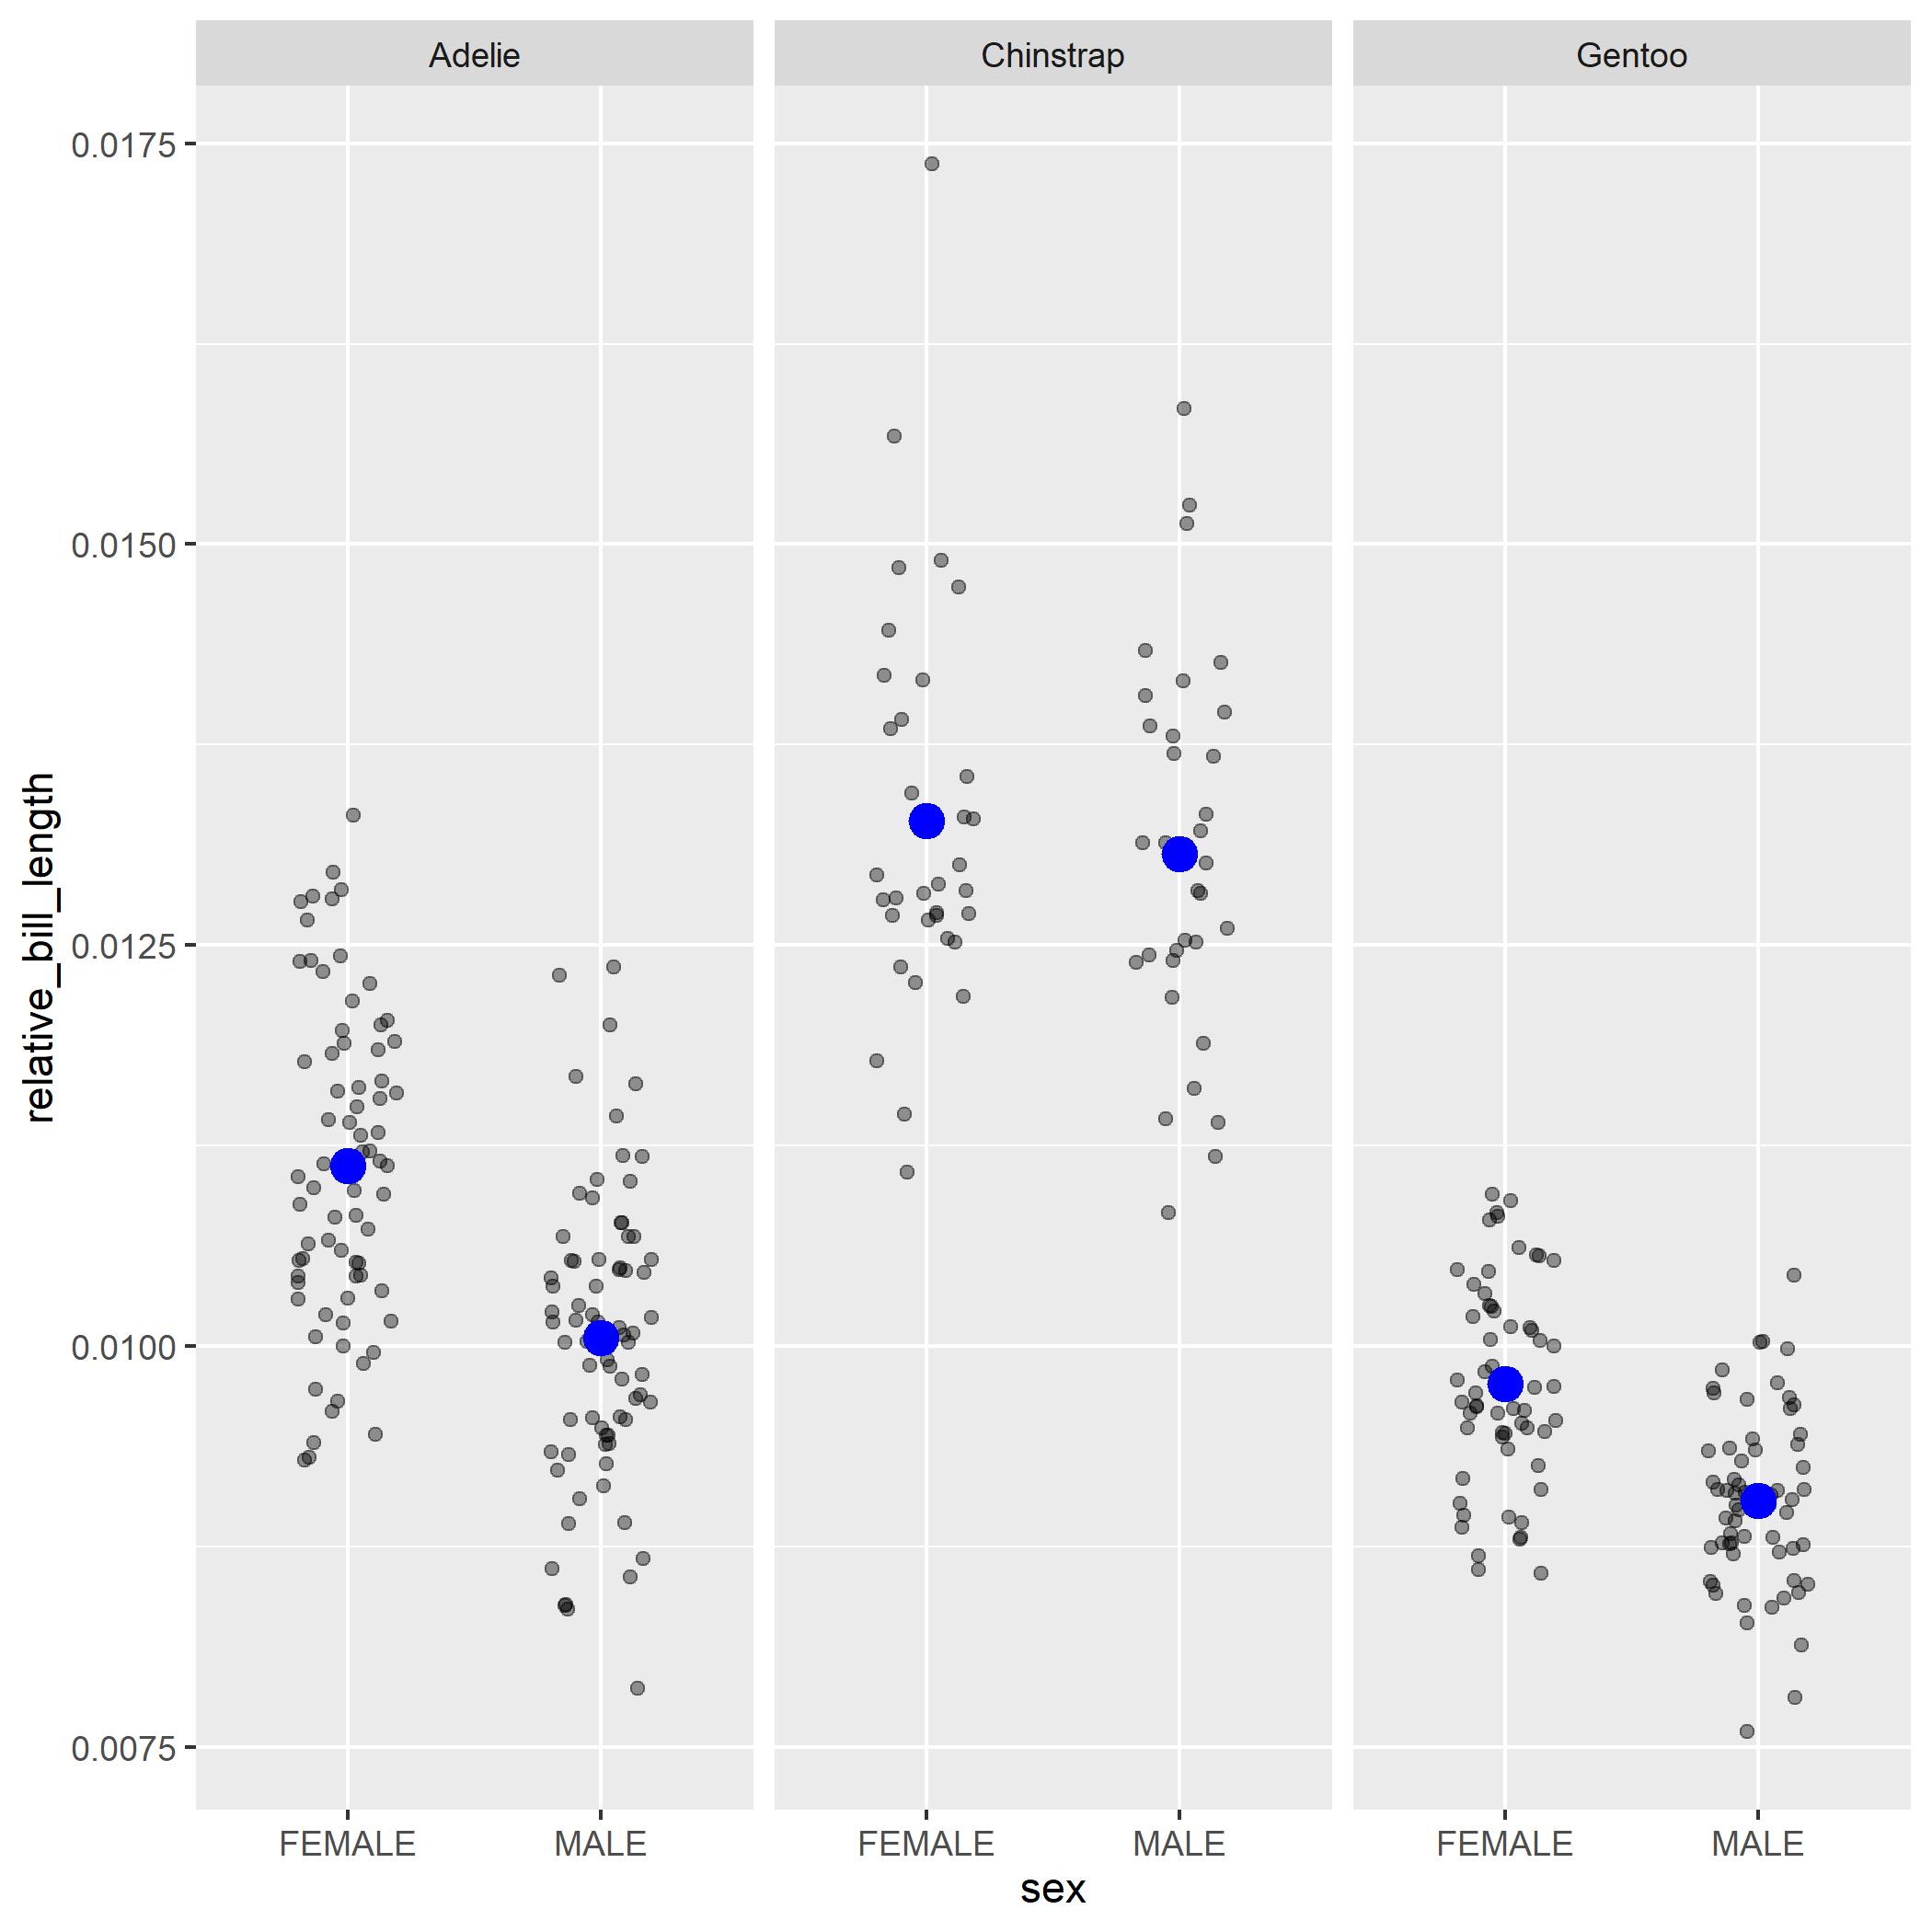
\includegraphics[width=1\linewidth]{images/bluedotplot}
\textgreater{} Note - we could be producing something much simpler, like a box and whisker plot. It is often better to plot the data points rather than summaries of them

Imagine a line connects the two blue dots in each facet, these blue dots are the mean values. The slope of the line (if we drew them) would be downwards from females to males, indicating that on average females are larger. But the slop would not be very large. If we drew slope between \emph{each} of the three female averages these would be much steeper. So we can say that size `on average' varies more \emph{between} species than \emph{between} sexes.

See if you can make figures for all four of our variables of interest, then compare them to our initial hypotheses.

At this stage we do not have enough evidence to formally ``reject'' any of our null hypotheses, however we can describe the trends which appear to be present.

\begin{figure}
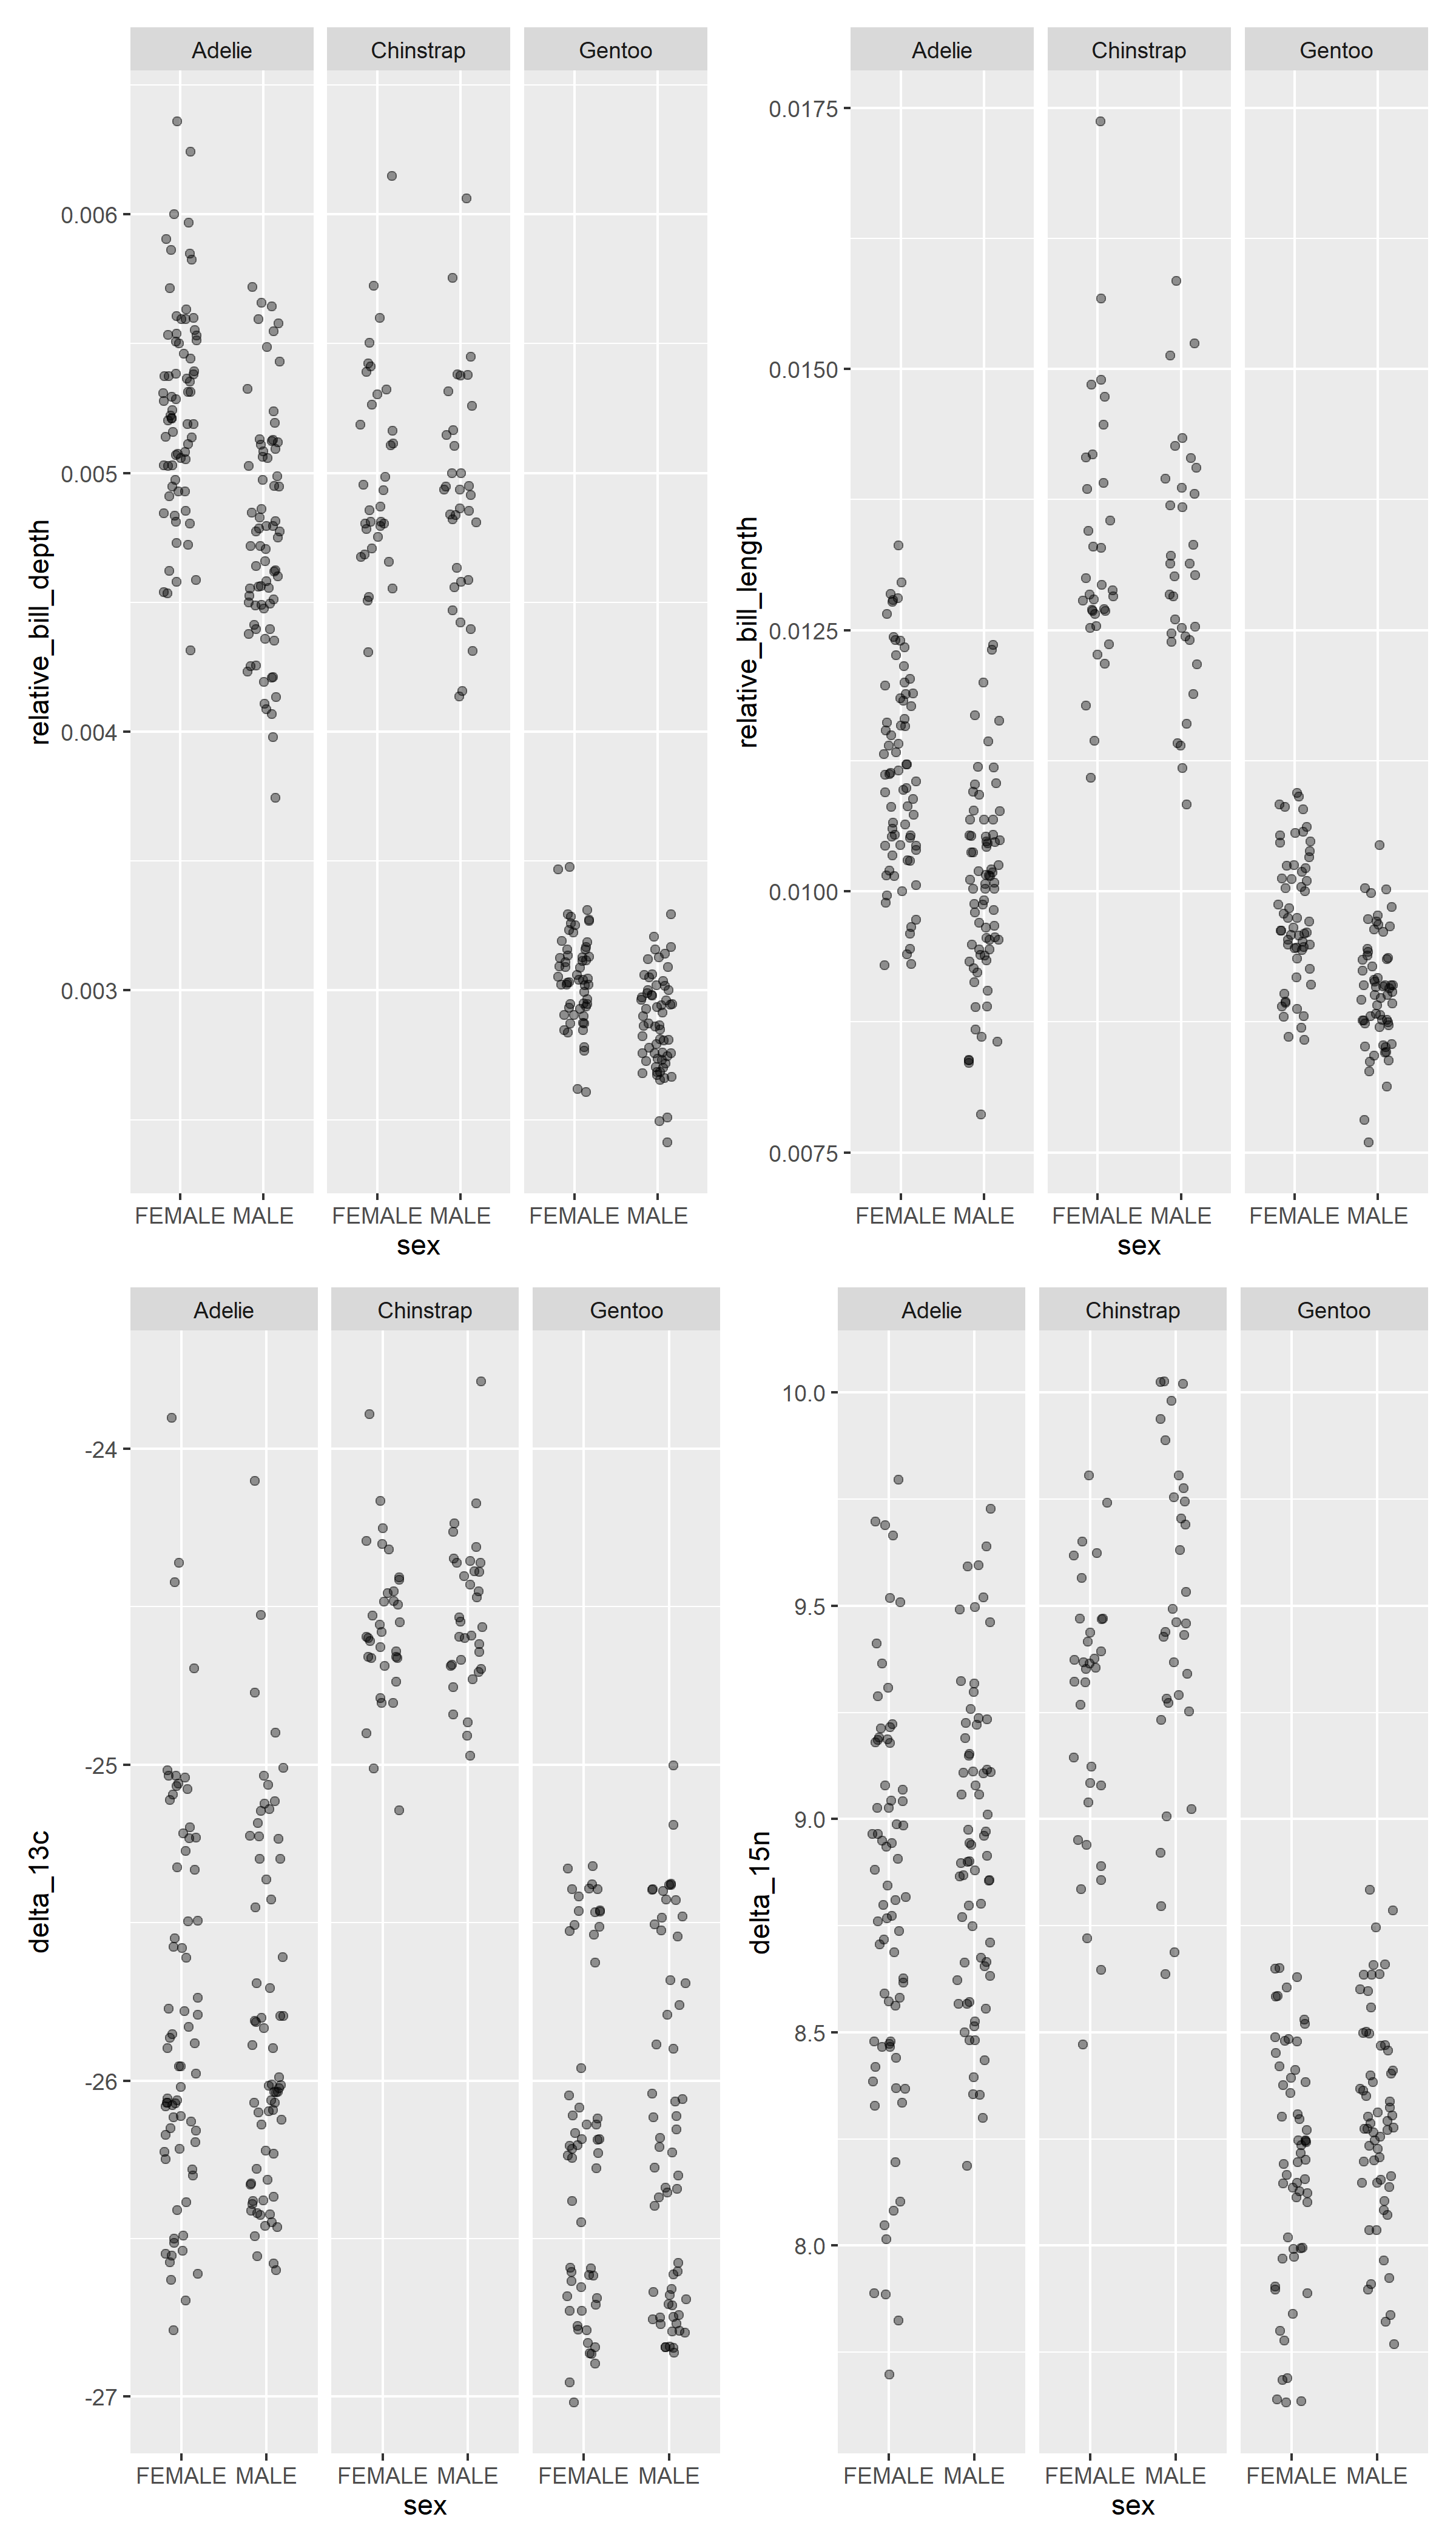
\includegraphics[width=0.8\linewidth]{images/summary} \caption{Difference in relative bill length and depth, and heavy carbon and nitrogen ratios, in male and female penguins from three different species - Adelie, Chinstrap and Gentoo}\label{fig:unnamed-chunk-111}
\end{figure}

\hypertarget{making-our-graphs-more-attractive}{%
\section{Making our graphs more attractive}\label{making-our-graphs-more-attractive}}

We will dive into making attractive ggplots in more detail later. But let's spend a little time now fixing some of the more serious issues with our figures.

The aim with making a good figure, is that it is:

\begin{itemize}
\item
  Accurate - the figure must present the data properly, and not distort or mislead
\item
  Beautiful - attractive figures will invite people to spend more time studying them
\item
  Clear - a good figure should be able to stand on its own - see the answer or insight without prompting from the text
\end{itemize}

There are lots of things we could change here, but we will stick with the basics for now. We will:

\begin{itemize}
\item
  Change the axis labels
\item
  Add some colours
\item
  Remove the grey background
\end{itemize}

\begin{Shaded}
\begin{Highlighting}[]
\NormalTok{penguins }\SpecialCharTok{\%\textgreater{}\%} 
    \FunctionTok{drop\_na}\NormalTok{(sex) }\SpecialCharTok{\%\textgreater{}\%} 
    \FunctionTok{ggplot}\NormalTok{(}\FunctionTok{aes}\NormalTok{(}\AttributeTok{x=}\NormalTok{sex, }
               \AttributeTok{y=}\NormalTok{relative\_bill\_depth,}
               \AttributeTok{colour=}\NormalTok{sex))}\SpecialCharTok{+}
    \FunctionTok{geom\_jitter}\NormalTok{(}\AttributeTok{position=}\FunctionTok{position\_jitter}\NormalTok{(}\AttributeTok{width=}\FloatTok{0.2}\NormalTok{), }
                \AttributeTok{alpha=}\FloatTok{0.4}\NormalTok{)}\SpecialCharTok{+}
  \FunctionTok{scale\_color\_manual}\NormalTok{(}\AttributeTok{values=}\FunctionTok{c}\NormalTok{(}\StringTok{"darkorange"}\NormalTok{, }\StringTok{"blue"}\NormalTok{))}\SpecialCharTok{+}
        \FunctionTok{facet\_wrap}\NormalTok{(}\SpecialCharTok{\textasciitilde{}}\NormalTok{species)}\SpecialCharTok{+}
  \FunctionTok{ylab}\NormalTok{(}\StringTok{"Culmen depth relative to body mass"}\NormalTok{)}\SpecialCharTok{+}
  \FunctionTok{xlab}\NormalTok{(}\StringTok{"Sex"}\NormalTok{)}\SpecialCharTok{+}
  \FunctionTok{scale\_x\_discrete}\NormalTok{(}\AttributeTok{labels=}\FunctionTok{c}\NormalTok{(}\StringTok{"Female"}\NormalTok{, }\StringTok{"Male"}\NormalTok{))}\SpecialCharTok{+}
  \FunctionTok{theme\_classic}\NormalTok{()}\SpecialCharTok{+}
  \FunctionTok{theme}\NormalTok{(}\AttributeTok{legend.position=}\StringTok{"none"}\NormalTok{)}
\end{Highlighting}
\end{Shaded}

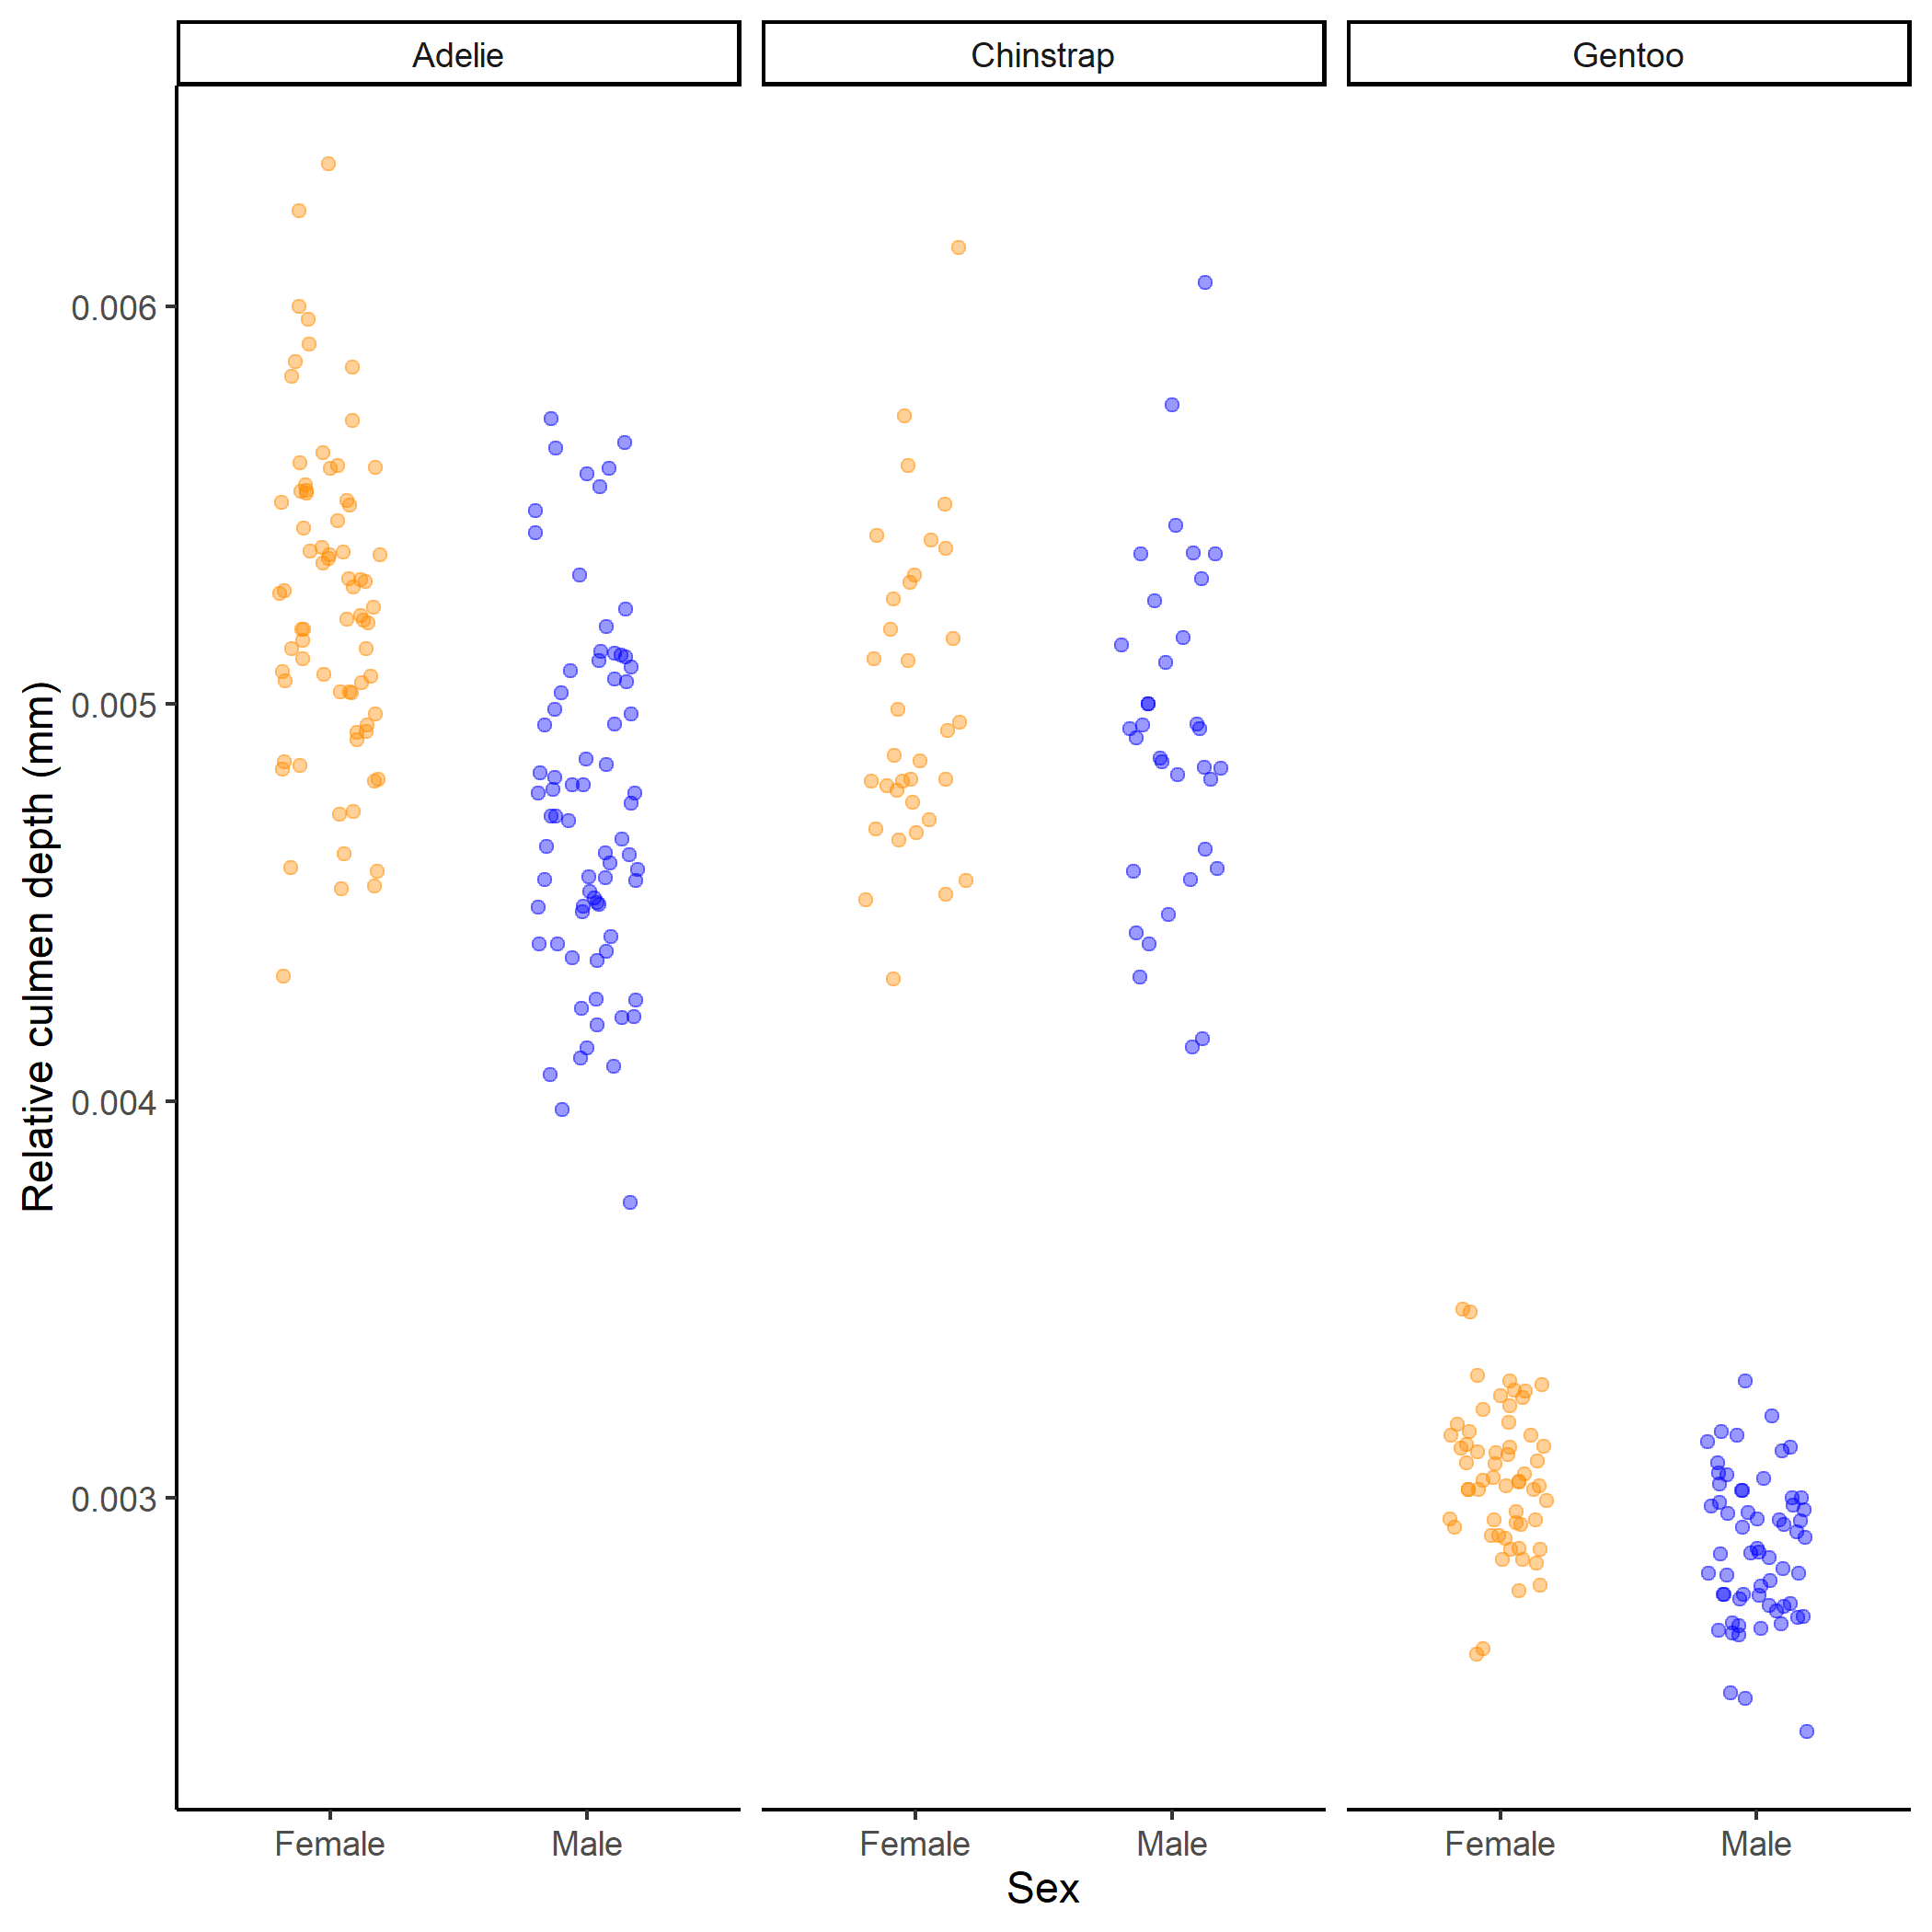
\includegraphics[width=0.8\linewidth]{images/final_figure_penguins}

\hypertarget{saving-your-output}{%
\subsection{Saving your output}\label{saving-your-output}}

Now we have made a plot, that perhaps we think is worth saving. We can use the \texttt{ggsave} function.
Just like when we imported data, when we output we specify a relative file path, this time we are saying where we want to `send' the output. At the start of our project set-up we made a folder for figures to end up.

\begin{Shaded}
\begin{Highlighting}[]
\CommentTok{\# save the last figure to a .png file in the figures folder}

\FunctionTok{ggsave}\NormalTok{(}\StringTok{"figures/Jitter plot of relative culmen depth.png"}\NormalTok{, }
       \AttributeTok{dpi=}\DecValTok{300}\NormalTok{, }\CommentTok{\# resolution}
       \AttributeTok{width=}\DecValTok{7}\NormalTok{, }\CommentTok{\# width in inches}
       \AttributeTok{height=}\DecValTok{7}\NormalTok{)}
\end{Highlighting}
\end{Shaded}

\begin{rmdwarning}
Be careful here, if you ran this command again it would overwrite your
previous file with a new output.
\end{rmdwarning}

Check your Files tab - your image file should be saved in the appropriate folder

\hypertarget{quitting-2}{%
\section{Quitting}\label{quitting-2}}

\begin{rmdwarning}
Make sure you have saved your script!
\end{rmdwarning}

\begin{rmdquestion}
Complete this week's Blackboard Quiz!
\end{rmdquestion}

\hypertarget{ggplot2-a-grammar-of-graphics-week-four}{%
\chapter{ggplot2 A grammar of graphics: Week Four}\label{ggplot2-a-grammar-of-graphics-week-four}}

\hypertarget{intro-to-grammar}{%
\section{Intro to grammar}\label{intro-to-grammar}}

The ggplot2 package is widely used and valued for its simple, consistent approach to making plots.

The `grammar' of graphics relates to the different components of a plot that function like different parts of linguistic grammar. For example, all plots require axes, so the x and y axes form one part of the `language' of a plot. Similarly, all plots have data represented between the axes, often as points, lines or bars. The visual way that the data is represented forms another component of the grammar of graphics. Furthermore, the colour, shape or size of points and lines can be used to encode additional information in the plot. This information is usually clarified in a key, or legend, which can also be considered part of this `grammar'.

The most common components of a ggplot are:

\begin{itemize}
\item
  aesthetics
\item
  geometric representations
\item
  facets
\item
  coordinate space
\item
  coordinate labels
\item
  plot theme
\end{itemize}

We will cover each below.

The philosophy of ggplot is much better explained by the package author, Hadley Wickham (\citet{R-ggplot2}). For now, we just need to be aware that ggplots are constructed by specifying the different components that we want to display, based on underlying information in a data frame.

\hypertarget{building-a-plot}{%
\section{Building a plot}\label{building-a-plot}}

We are going to use the \emph{simple} penguin data set contained in the \texttt{palmerpenguins} package (\citet{R-palmerpenguins}).

\begin{rmdwarning}
Make sure you have a folder structure for your project - scripts - data
(won't be needed this week) - figures

Make sure your new script is in the scripts folder!

Throughout this practical you will be introduced to new R packages.
Please remember to include all the library() calls at the TOP of your
script.

And if you need to install a package, the command is
`install.packages("") - but DON'T include this in your script
\end{rmdwarning}

\begin{Shaded}
\begin{Highlighting}[]
\FunctionTok{library}\NormalTok{(palmerpenguins)}
\end{Highlighting}
\end{Shaded}

Let's check the first 6 rows of information contained in the data frame, using the head() function:

\begin{Shaded}
\begin{Highlighting}[]
\FunctionTok{head}\NormalTok{(penguins)}
\end{Highlighting}
\end{Shaded}

\begin{verbatim}
# A tibble: 344 x 8
   species island    bill_length_mm bill_depth_mm flipper_length_mm body_mass_g sex     year
   <fct>   <fct>              <dbl>         <dbl>             <int>       <int> <fct>  <int>
 1 Adelie  Torgersen           39.1          18.7               181        3750 male    2007
 2 Adelie  Torgersen           39.5          17.4               186        3800 female  2007
 3 Adelie  Torgersen           40.3          18                 195        3250 female  2007
 4 Adelie  Torgersen           NA            NA                  NA          NA NA      2007
 5 Adelie  Torgersen           36.7          19.3               193        3450 female  2007
 6 Adelie  Torgersen           39.3          20.6               190        3650 male    2007
 7 Adelie  Torgersen           38.9          17.8               181        3625 female  2007
 8 Adelie  Torgersen           39.2          19.6               195        4675 male    2007
 9 Adelie  Torgersen           34.1          18.1               193        3475 NA      2007
10 Adelie  Torgersen           42            20.2               190        4250 NA      2007
# ... with 334 more rows
\end{verbatim}

Here, we aim to produce a scatter plot

\hypertarget{plot-background}{%
\section{Plot background}\label{plot-background}}

To start building the plot, we first specify the data frame that contains the relevant data. We can do this in two ways

\begin{enumerate}
\def\labelenumi{\arabic{enumi})}
\tightlist
\item
  Here we are `sending the penguins data set into the ggplot function':
\end{enumerate}

\begin{Shaded}
\begin{Highlighting}[]
\CommentTok{\# render the plot background}
\NormalTok{penguins }\SpecialCharTok{\%\textgreater{}\%} 
  \FunctionTok{ggplot}\NormalTok{()}
\end{Highlighting}
\end{Shaded}

\begin{enumerate}
\def\labelenumi{\arabic{enumi})}
\setcounter{enumi}{1}
\tightlist
\item
  Here we are specifying the dataframe \emph{within} the \texttt{ggplot()} function
\end{enumerate}

\begin{Shaded}
\begin{Highlighting}[]
\FunctionTok{ggplot}\NormalTok{(}\AttributeTok{data=}\NormalTok{penguins)}
\end{Highlighting}
\end{Shaded}

The output is identical


\includegraphics[width=0.8\linewidth]{images/empty}
\textgreater{} **Note - Running this command will produce an empty grey panel. This is because we need to specify how different columns of the data frame should be represented in the plot.

\hypertarget{aesthetics---aes}{%
\section{Aesthetics - aes()}\label{aesthetics---aes}}

We can call in different columns of data from any dataset based on their column names. Column names are given as `aesthetic' elements to the ggplot function, and are wrapped in the aes() function.

Because we want a scatter plot, each point will have an x and a y coordinate. We want the x axis to represent flipper length ( x = flipper\_length\_mm ), and the y axis to represent the body mass ( y = body\_mass\_g ).

We give these specifications separated by a comma. Quotes are not required when giving variables within aes().

\begin{quote}
**Note - Those interested in why quotes aren't required can read about {[}non-standard evaluation{]} (\url{https://edwinth.github.io/blog/nse/}).
\end{quote}

\begin{Shaded}
\begin{Highlighting}[]
\NormalTok{penguins }\SpecialCharTok{\%\textgreater{}\%} 
  \FunctionTok{ggplot}\NormalTok{(}\FunctionTok{aes}\NormalTok{(}\AttributeTok{x=}\NormalTok{flipper\_length\_mm, }
             \AttributeTok{y =}\NormalTok{ body\_mass\_g))}
\end{Highlighting}
\end{Shaded}

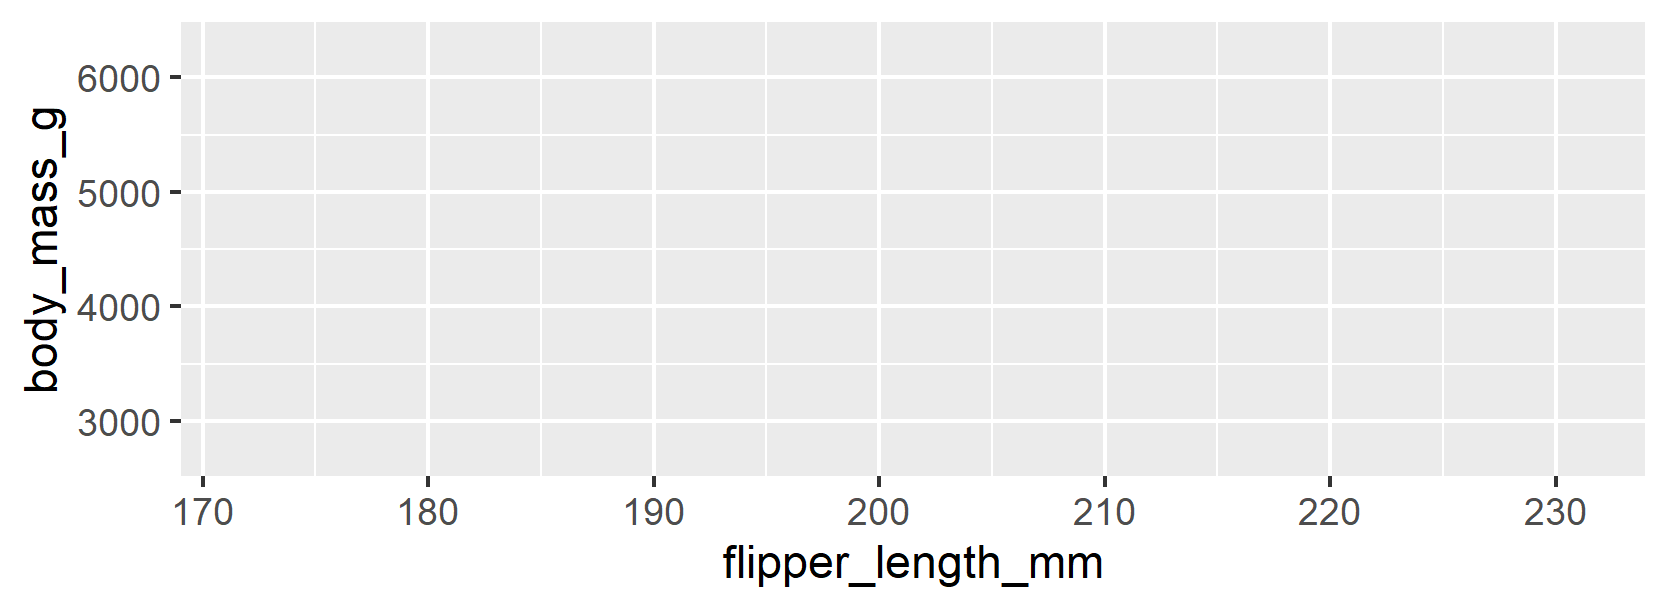
\includegraphics[width=0.8\linewidth]{images/axes}
So far we have the grid lines for our x and y axis. ggplot knows the variables required for the plot, and thus the scale, but has no information about how to display the data points.

\hypertarget{geometric-representations---geom}{%
\section{Geometric representations - geom()}\label{geometric-representations---geom}}

Given we want a scatter plot, we need to specify that the geometric representation of the data will be in point form, using geom\_point().

Here we are adding a layer (hence the + sign) of points to the plot. We can think of this as similar to e.g.~Adobe Photoshop which uses layers of images that can be reordered and modified individually. Because we add to plots layer by layer \textbf{the order} of your geoms may be important for your final aesthetic design.

For ggplot, each layer will be added over the plot according to its position in the code. Below I first show the full breakdown of the components in a layer. Each layer requires information on

\begin{itemize}
\tightlist
\item
  data
\item
  aesthetics
\item
  geometric type
\item
  any summary of the data
\item
  position
\end{itemize}

\begin{Shaded}
\begin{Highlighting}[]
\NormalTok{penguins }\SpecialCharTok{\%\textgreater{}\%} 
  \FunctionTok{ggplot}\NormalTok{(}\FunctionTok{aes}\NormalTok{(}\AttributeTok{x=}\NormalTok{flipper\_length\_mm, }
             \AttributeTok{y =}\NormalTok{ body\_mass\_g))}\SpecialCharTok{+}
  \FunctionTok{layer}\NormalTok{(                }\CommentTok{\# layer inherits data and aesthetic arguments from previous}
    \AttributeTok{geom=}\StringTok{"point"}\NormalTok{,       }\CommentTok{\# draw point objects}
    \AttributeTok{stat=}\StringTok{"identity"}\NormalTok{,    }\CommentTok{\# each individual data point gets a geom (no summaries)}
    \AttributeTok{position=}\FunctionTok{position\_identity}\NormalTok{()) }\CommentTok{\# data points are not moved in any way e.g. we could specify jitter or dodge if we want to avoid busy overlapping data}
\end{Highlighting}
\end{Shaded}

This is quite a complicate way to write new layers - and it is more usual to see a simpler more compact approach

\begin{Shaded}
\begin{Highlighting}[]
\NormalTok{penguins }\SpecialCharTok{\%\textgreater{}\%} 
  \FunctionTok{ggplot}\NormalTok{(}\FunctionTok{aes}\NormalTok{(}\AttributeTok{x=}\NormalTok{flipper\_length\_mm, }
             \AttributeTok{y =}\NormalTok{ body\_mass\_g))}\SpecialCharTok{+}
  \FunctionTok{geom\_point}\NormalTok{() }\CommentTok{\# geom\_point function will always draw points, and unless specified otherwise the arguments for position and stat are both "identity".}
\end{Highlighting}
\end{Shaded}

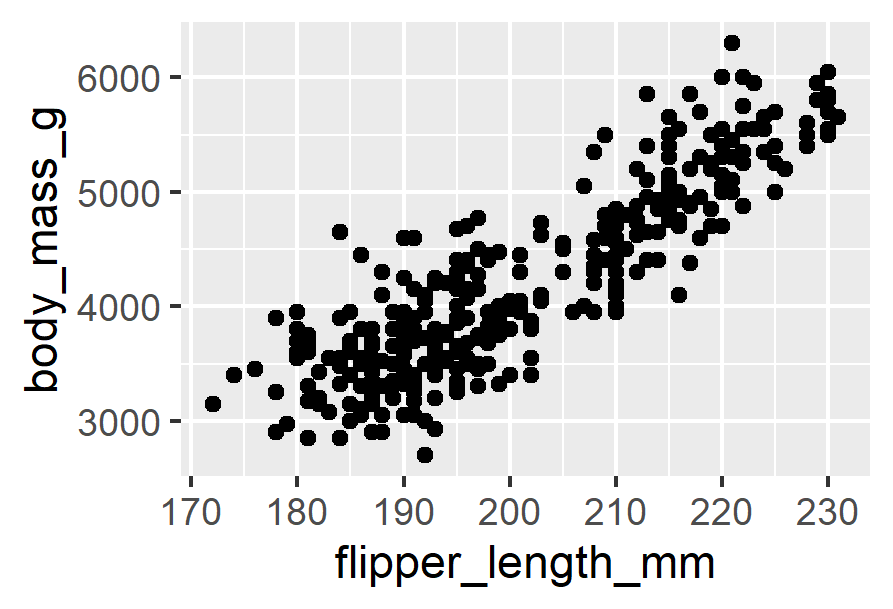
\includegraphics[width=0.8\linewidth]{images/simplepoints}

Now we have the scatter plot! Each row (except for two rows of missing data) in the penguins data set now has an x coordinate, a y coordinate, and a designated geometric representation (point).

From this we can see that smaller penguins tend to have smaller flipper lengths.

\hypertarget{and}{%
\section{\%\textgreater\% and +}\label{and}}

ggplot2, an early component of the tidyverse package, was written before the pipe was introduced. The + sign in ggplot2 functions in a similar way to the pipe in other functions in the tidyverse: by allowing code to be written from left to right.

\hypertarget{colour}{%
\section{Colour}\label{colour}}

The current plot could be more informative, to include information about the species of each penguin.

In order to achieve this we need to use aes() again, and specify which column we want to be represented as the colour of the points.
Here, the aes() function containing the relevant column name, is given within the geom\_point() function.

\begin{Shaded}
\begin{Highlighting}[]
\NormalTok{penguins }\SpecialCharTok{\%\textgreater{}\%} 
  \FunctionTok{ggplot}\NormalTok{(}\FunctionTok{aes}\NormalTok{(}\AttributeTok{x=}\NormalTok{flipper\_length\_mm, }
             \AttributeTok{y =}\NormalTok{ body\_mass\_g))}\SpecialCharTok{+}
  \FunctionTok{geom\_point}\NormalTok{(}\FunctionTok{aes}\NormalTok{(}\AttributeTok{colour=}\NormalTok{species))}
\end{Highlighting}
\end{Shaded}

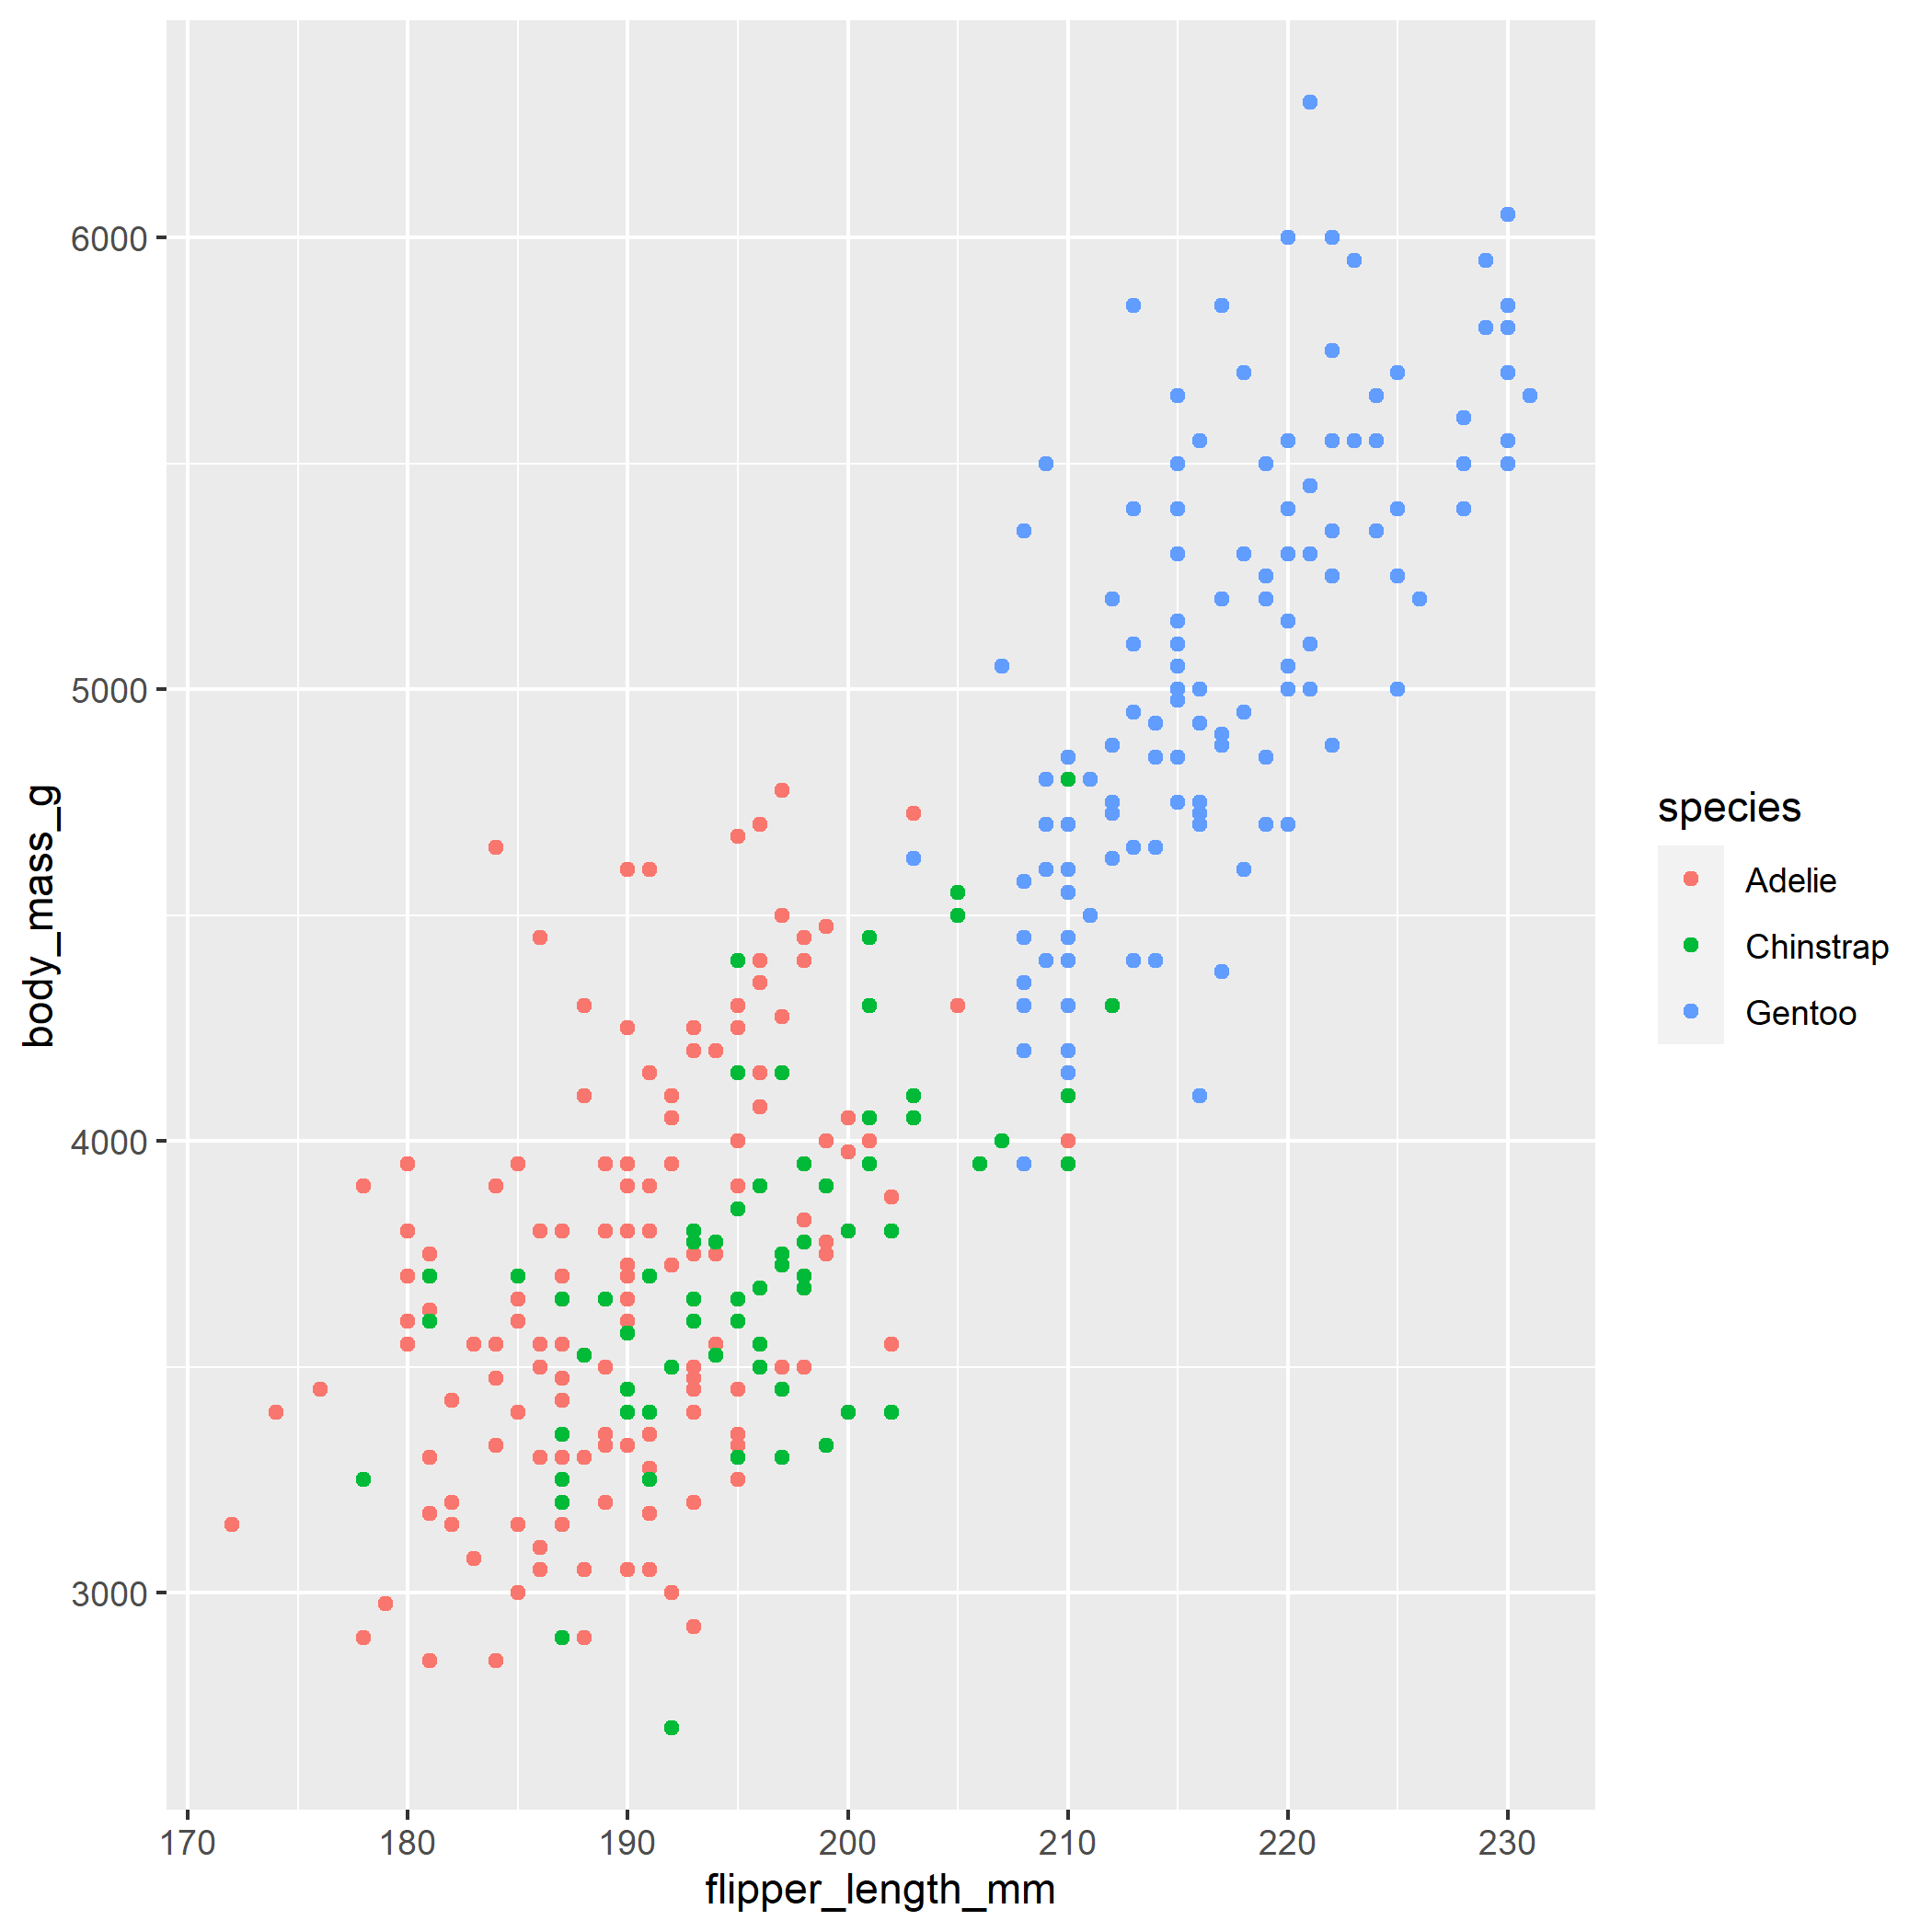
\includegraphics[width=0.8\linewidth]{images/colourpoints}

\begin{quote}
**Note - you may (or may not) have noticed that the grammar of ggplot (and tidyverse in general) accepts British/Americanization for spelling!!!
\end{quote}

So now we can see that the Gentoo penguins tend to be both larger and have longer flippers

Remember to keep adding carriage returns (new lines), which must be inserted after the \%\textgreater\% or + symbols.
In most cases, R is blind to white space and new lines, so this is simply to make our code more readable, and allow us to add readable comments.

\hypertarget{more-layers}{%
\section{More layers}\label{more-layers}}

We can see the relationship between body size and flipper length. But what if we want to model this relationship with a trend line? We can add another `layer' to this plot, using a different geometric representation of the data. In this case a trend line, which is in fact a summary of the data rather than a representation of each point.

The geom\_smooth() function draws a trend line through the data. The default behaviour is to draw a local regression line (curve) through the points, however these can be hard to interpret. We want to add a straight line based on a linear model (`lm') of the relationship between x and y.

This is our \textbf{first} encounter with linear models in this course, but we will learn a lot more about them later on.

\begin{Shaded}
\begin{Highlighting}[]
\NormalTok{penguins }\SpecialCharTok{\%\textgreater{}\%} 
  \FunctionTok{ggplot}\NormalTok{(}\FunctionTok{aes}\NormalTok{(}\AttributeTok{x=}\NormalTok{flipper\_length\_mm, }
             \AttributeTok{y =}\NormalTok{ body\_mass\_g))}\SpecialCharTok{+}
  \FunctionTok{geom\_point}\NormalTok{(}\FunctionTok{aes}\NormalTok{(}\AttributeTok{colour=}\NormalTok{species))}\SpecialCharTok{+}
  \FunctionTok{geom\_smooth}\NormalTok{(}\AttributeTok{method=}\StringTok{"lm"}\NormalTok{,    }\CommentTok{\#add another layer of data representation.}
              \AttributeTok{se=}\ConstantTok{FALSE}\NormalTok{,}
              \FunctionTok{aes}\NormalTok{(}\AttributeTok{colour=}\NormalTok{species)) }\CommentTok{\# note layers inherit information from the top ggplot() function but not previous layers {-} if we want separate lines per species we need to either specify this again *or* move the color aesthetic to the top layer. }
\end{Highlighting}
\end{Shaded}

\begin{Shaded}
\begin{Highlighting}[]
\NormalTok{penguins }\SpecialCharTok{\%\textgreater{}\%} 
  \FunctionTok{ggplot}\NormalTok{(}\FunctionTok{aes}\NormalTok{(}\AttributeTok{x=}\NormalTok{flipper\_length\_mm, }
             \AttributeTok{y =}\NormalTok{ body\_mass\_g,}
             \AttributeTok{colour=}\NormalTok{species))}\SpecialCharTok{+} \DocumentationTok{\#\#\# now colour is set here it will be inherited by ALL layers}
  \FunctionTok{geom\_point}\NormalTok{()}\SpecialCharTok{+}
  \FunctionTok{geom\_smooth}\NormalTok{(}\AttributeTok{method=}\StringTok{"lm"}\NormalTok{,    }\CommentTok{\#add another layer of data representation.}
              \AttributeTok{se=}\ConstantTok{FALSE}\NormalTok{)}
\end{Highlighting}
\end{Shaded}

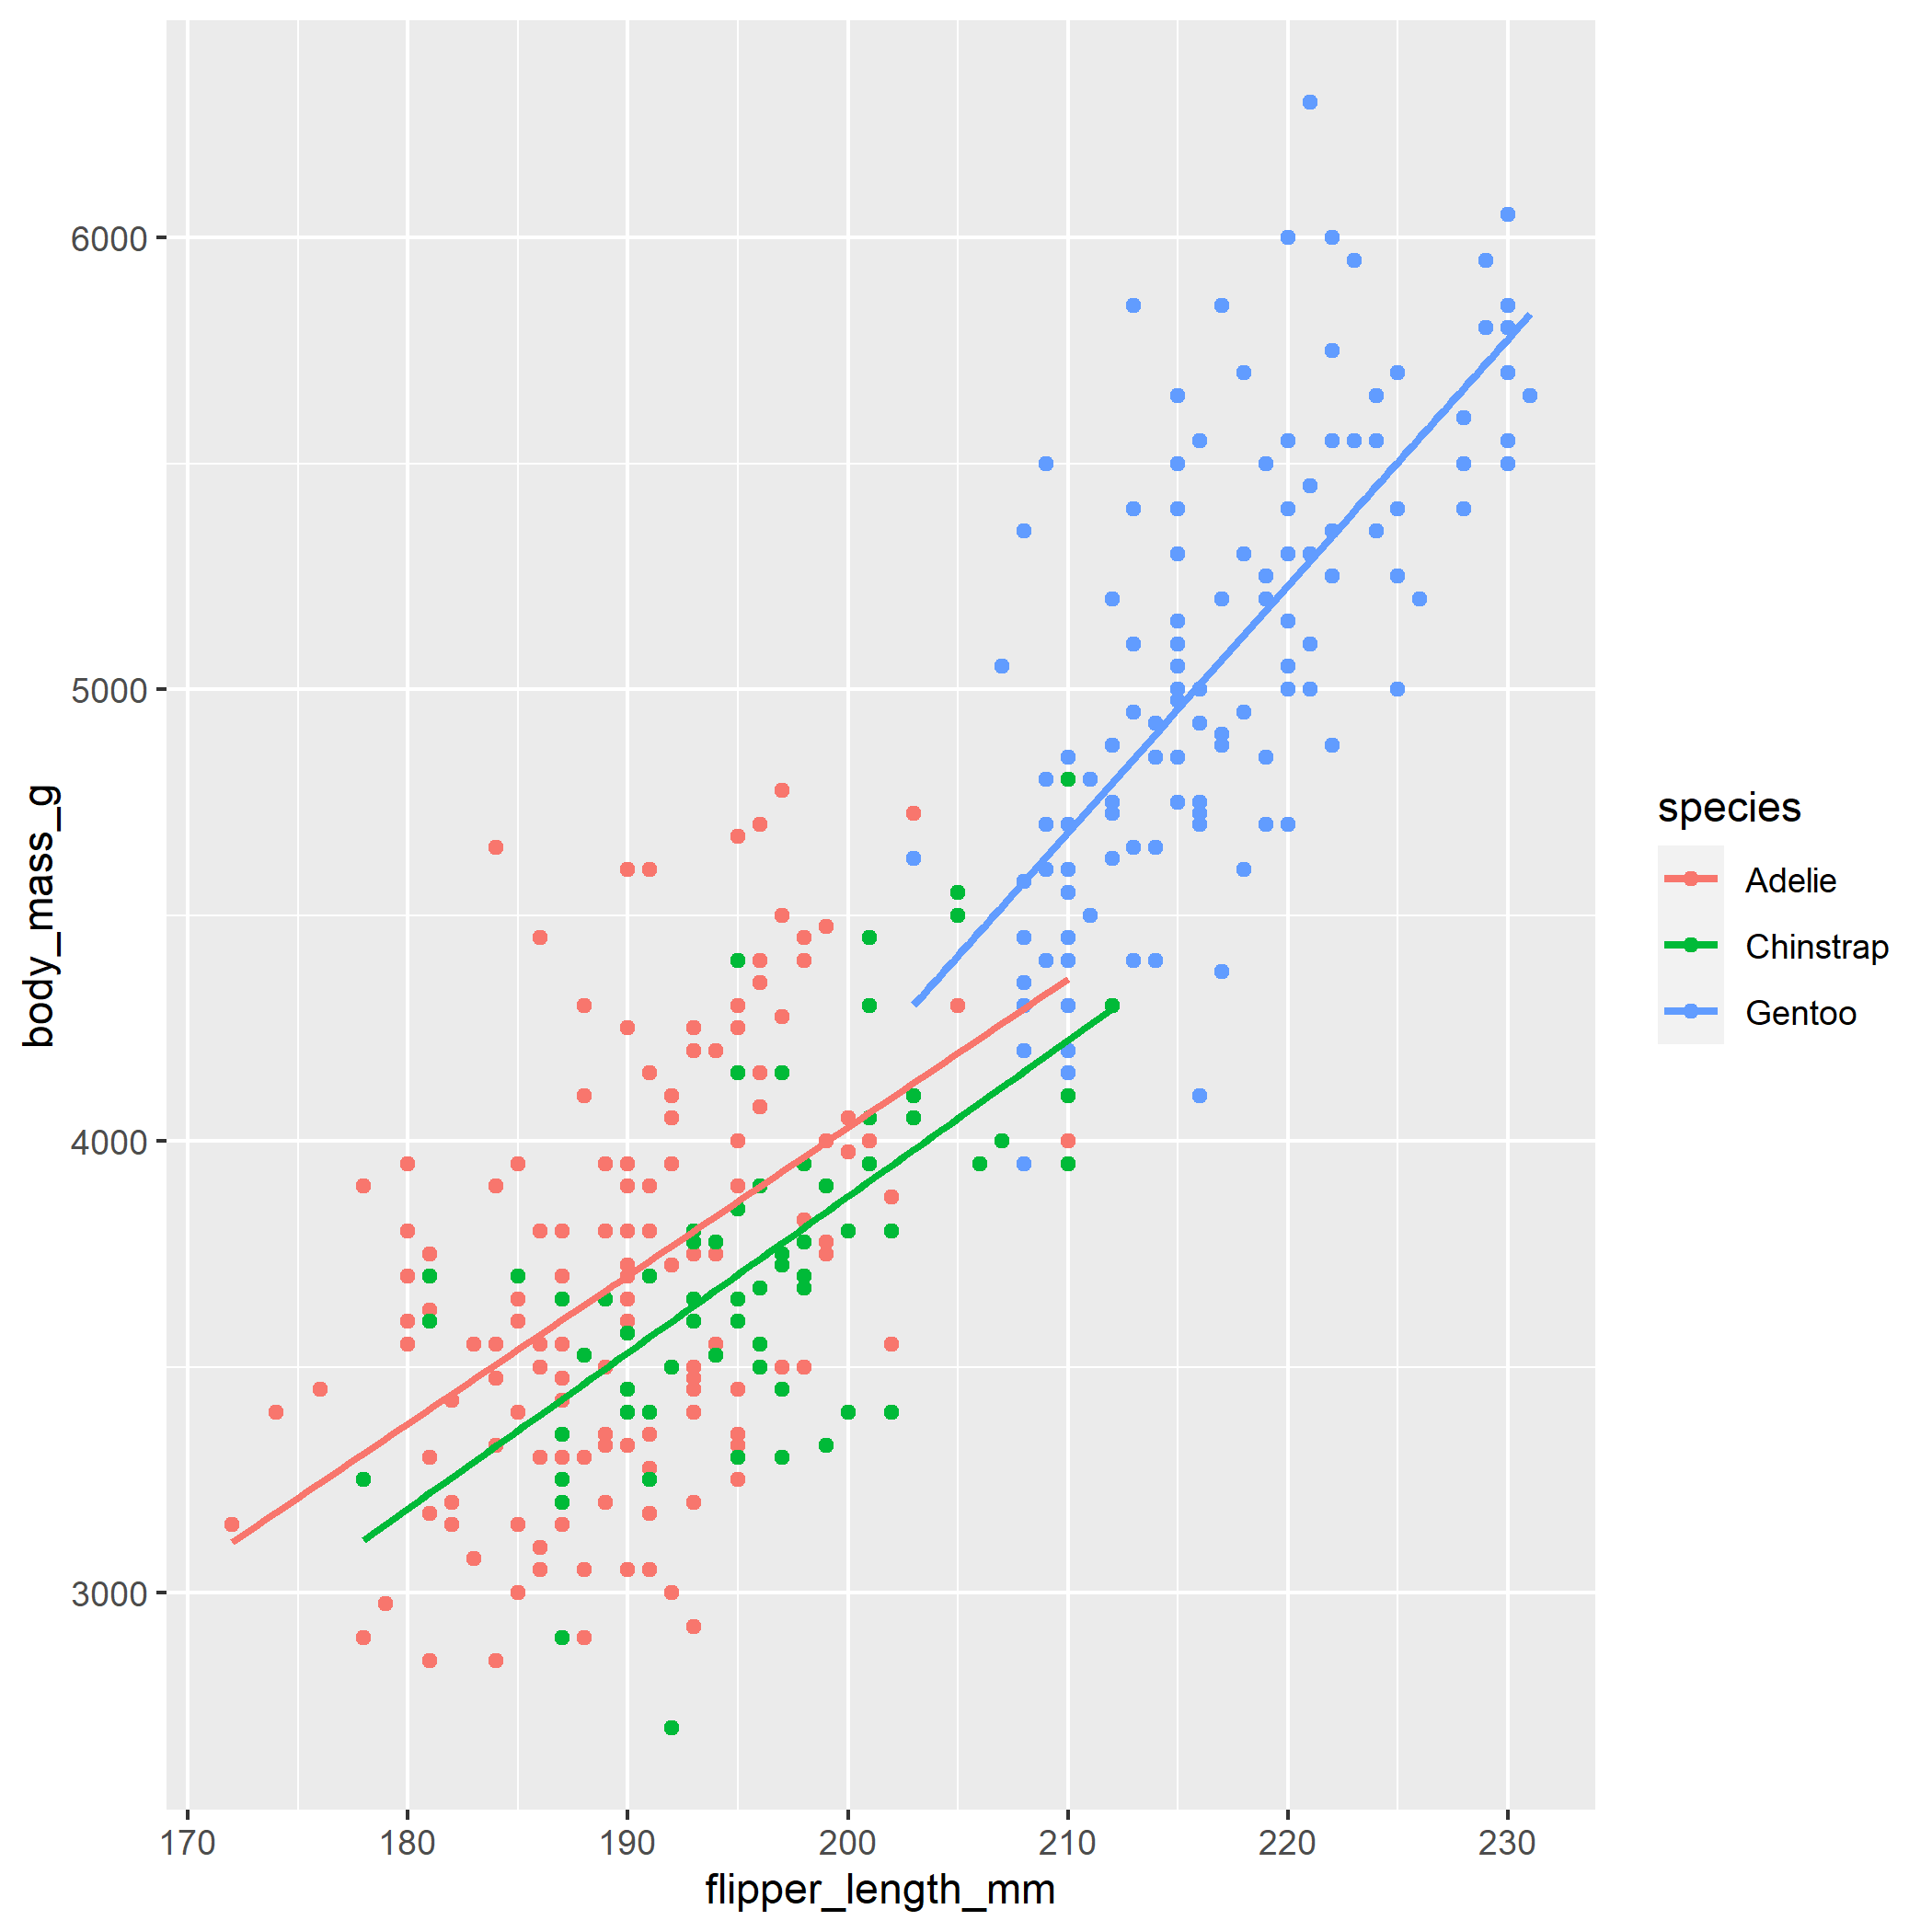
\includegraphics[width=0.8\linewidth]{images/linearmodel}
\textgreater{} **Note - that the trend line is blocking out certain points, because it is the `top layer' of the plot. The geom layers that appear early in the command are drawn first, and can be obscured by the geom layers that come after them.

\begin{rmdquestion}
What happens if you switch the order of the geom\_point() and
geom\_smooth() functions above? What do you notice about the trend line?
\end{rmdquestion}

\hypertarget{facets}{%
\section{Facets}\label{facets}}

In some cases we want to break up a single plot into sub-plots, called `faceting'. Facets are commonly used when there is too much data to display clearly in a single plot. We will revisit faceting below, however for now, let's try to facet the plot according to species.
To do this we use the tilde symbol `\textasciitilde{}' to indicate the column name that will form each facet.

\begin{Shaded}
\begin{Highlighting}[]
\NormalTok{penguins }\SpecialCharTok{\%\textgreater{}\%} 
  \FunctionTok{ggplot}\NormalTok{(}\FunctionTok{aes}\NormalTok{(}\AttributeTok{x=}\NormalTok{flipper\_length\_mm, }
             \AttributeTok{y =}\NormalTok{ body\_mass\_g,}
             \AttributeTok{colour=}\NormalTok{species))}\SpecialCharTok{+} 
  \FunctionTok{geom\_point}\NormalTok{()}\SpecialCharTok{+}
  \FunctionTok{geom\_smooth}\NormalTok{(}\AttributeTok{method=}\StringTok{"lm"}\NormalTok{,    }
              \AttributeTok{se=}\ConstantTok{FALSE}\NormalTok{)}\SpecialCharTok{+}
  \FunctionTok{facet\_wrap}\NormalTok{(}\SpecialCharTok{\textasciitilde{}}\NormalTok{species)}
\end{Highlighting}
\end{Shaded}

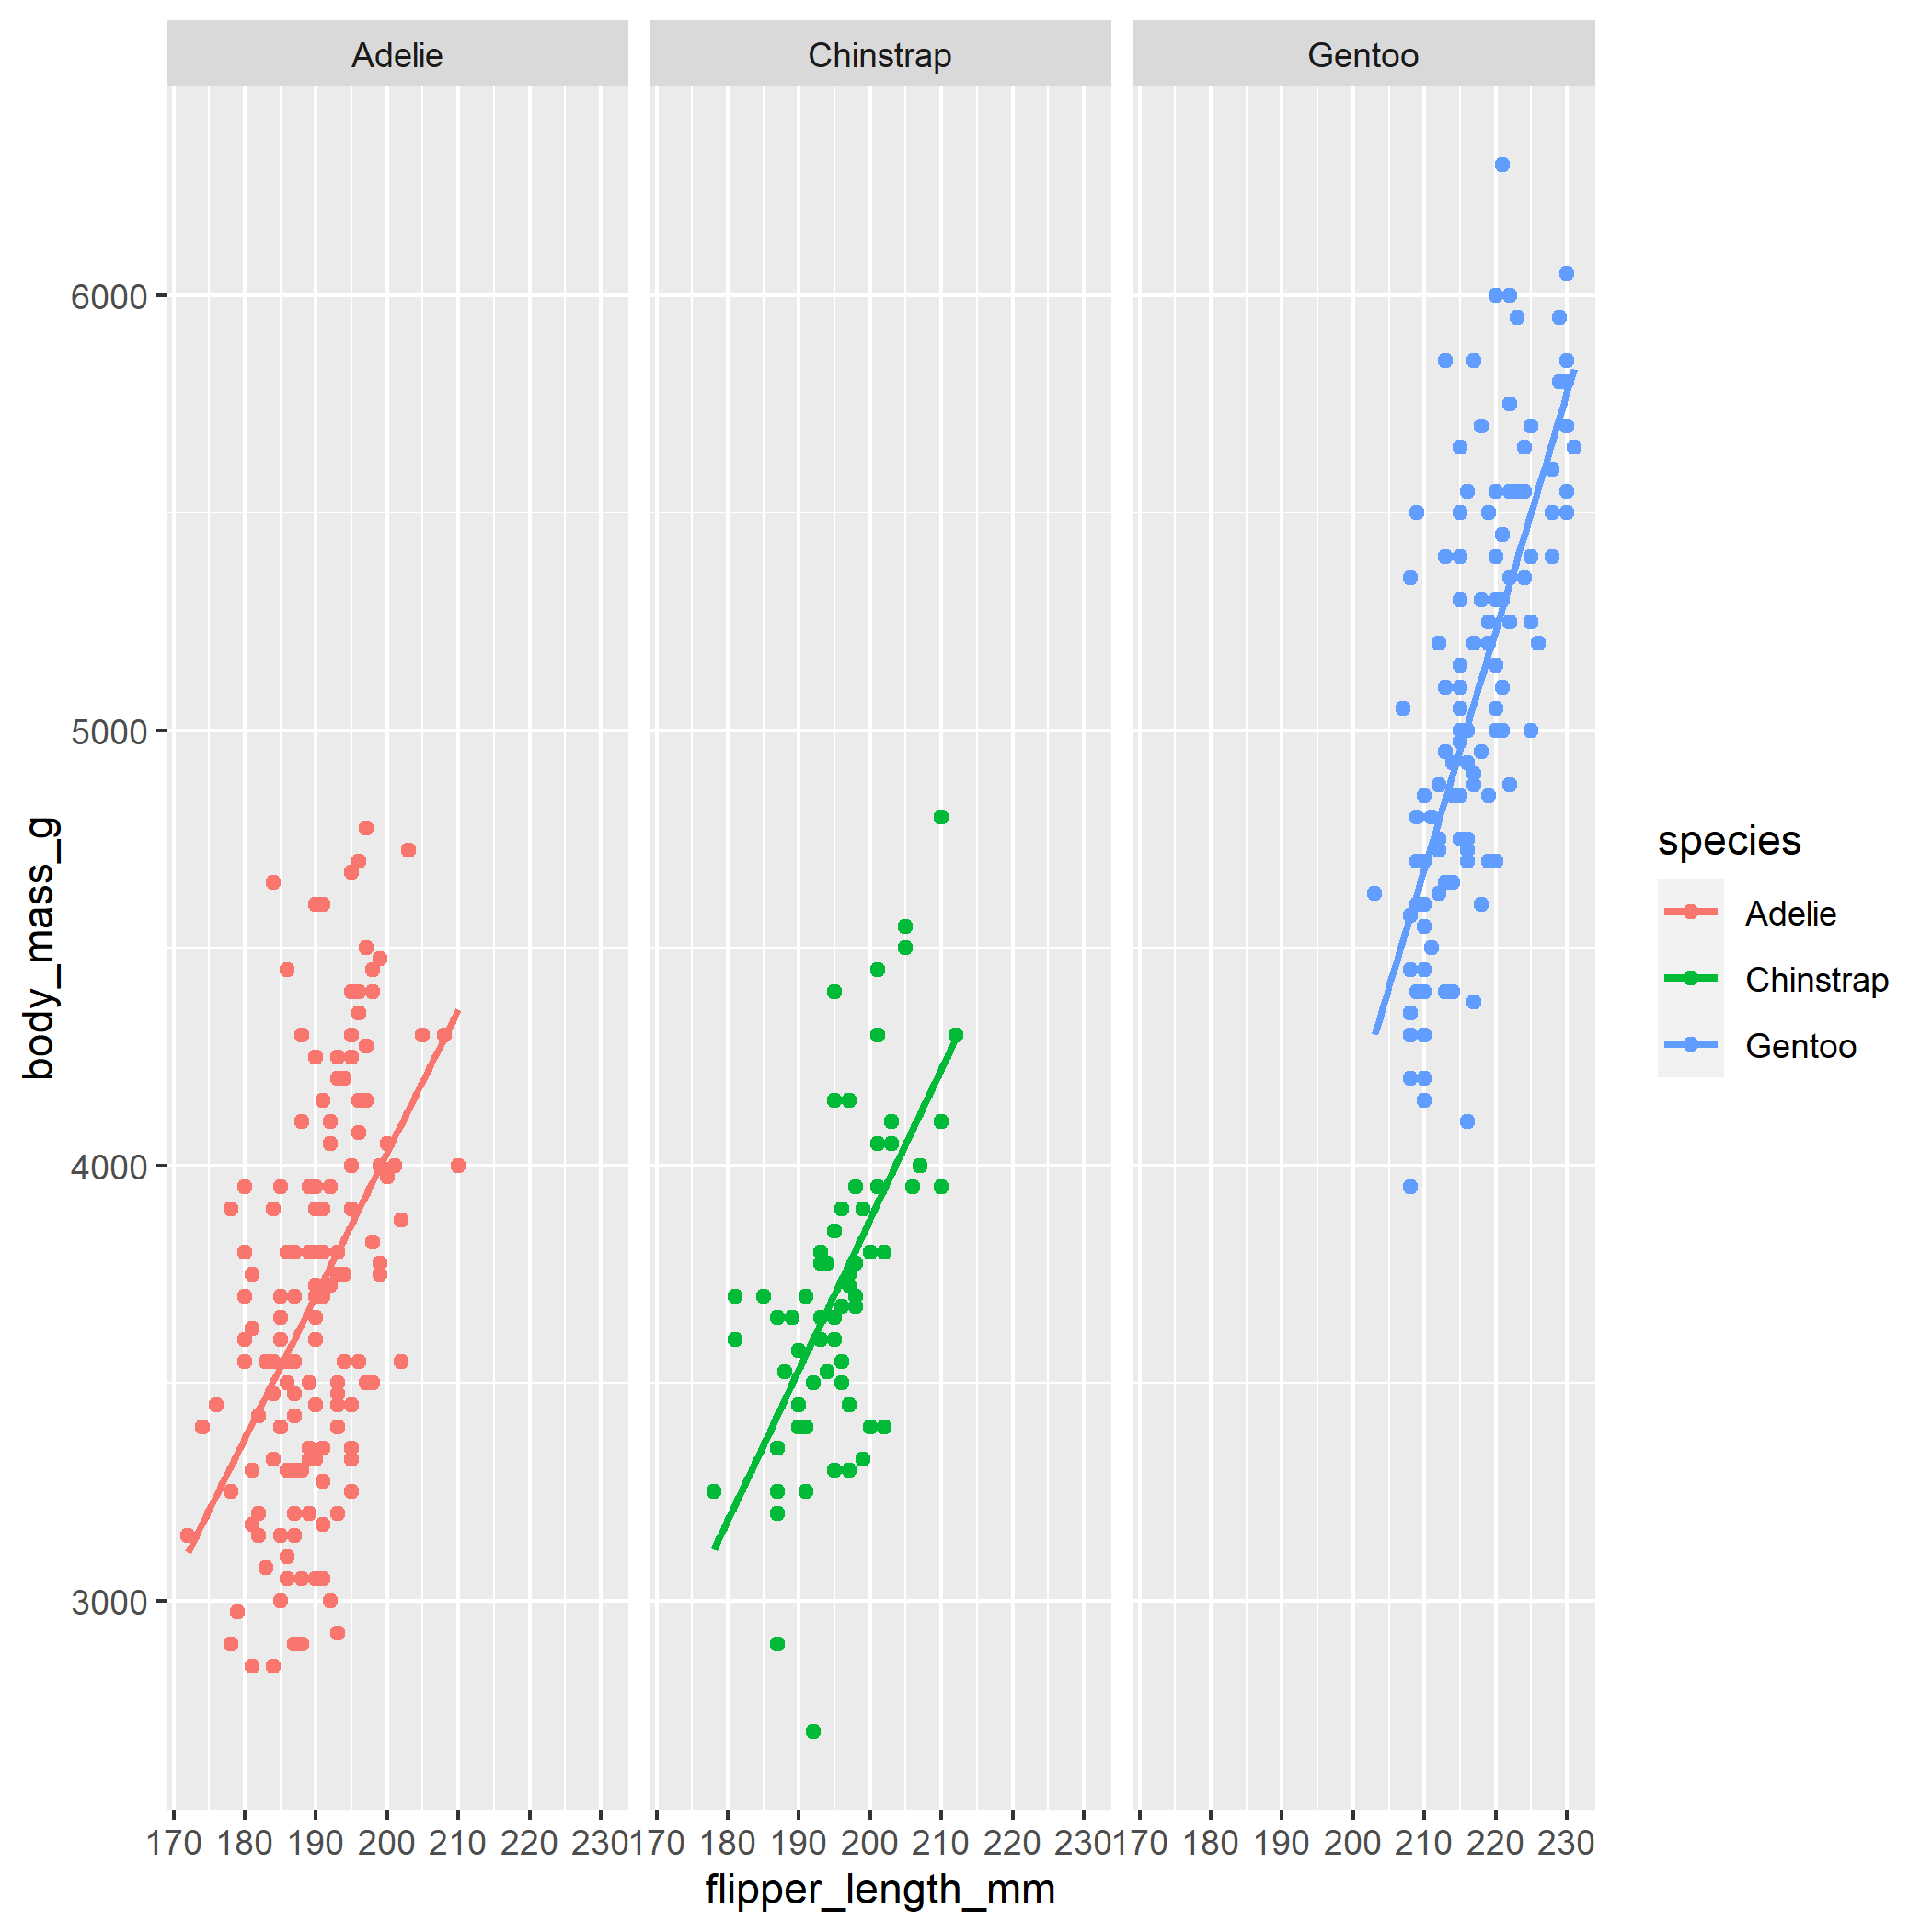
\includegraphics[width=0.8\linewidth]{images/facet}

\begin{quote}
**Note - the aesthetics and geoms including the regression line that were specified for the original plot, are applied to each of the facets.
\end{quote}

\hypertarget{co-ordinate-space}{%
\section{Co-ordinate space}\label{co-ordinate-space}}

ggplot will automatically pick the scale for each axis, and the type of coordinate space. Most plots are in Cartesian (linear X vs linear Y) coordinate space.

For this plot, let's say we want the x and y origin to be set at 0. To do this we can add in xlim() and ylim() functions, which define the limits of the axes:

\begin{Shaded}
\begin{Highlighting}[]
\NormalTok{penguins }\SpecialCharTok{\%\textgreater{}\%} 
  \FunctionTok{ggplot}\NormalTok{(}\FunctionTok{aes}\NormalTok{(}\AttributeTok{x=}\NormalTok{flipper\_length\_mm, }
             \AttributeTok{y =}\NormalTok{ body\_mass\_g,}
             \AttributeTok{colour=}\NormalTok{species))}\SpecialCharTok{+} 
  \FunctionTok{geom\_point}\NormalTok{()}\SpecialCharTok{+}
  \FunctionTok{geom\_smooth}\NormalTok{(}\AttributeTok{method=}\StringTok{"lm"}\NormalTok{,    }
              \AttributeTok{se=}\ConstantTok{FALSE}\NormalTok{)}\SpecialCharTok{+}
  \FunctionTok{xlim}\NormalTok{(}\DecValTok{0}\NormalTok{,}\DecValTok{240}\NormalTok{) }\SpecialCharTok{+} \FunctionTok{ylim}\NormalTok{(}\DecValTok{0}\NormalTok{,}\DecValTok{7000}\NormalTok{)}
\end{Highlighting}
\end{Shaded}

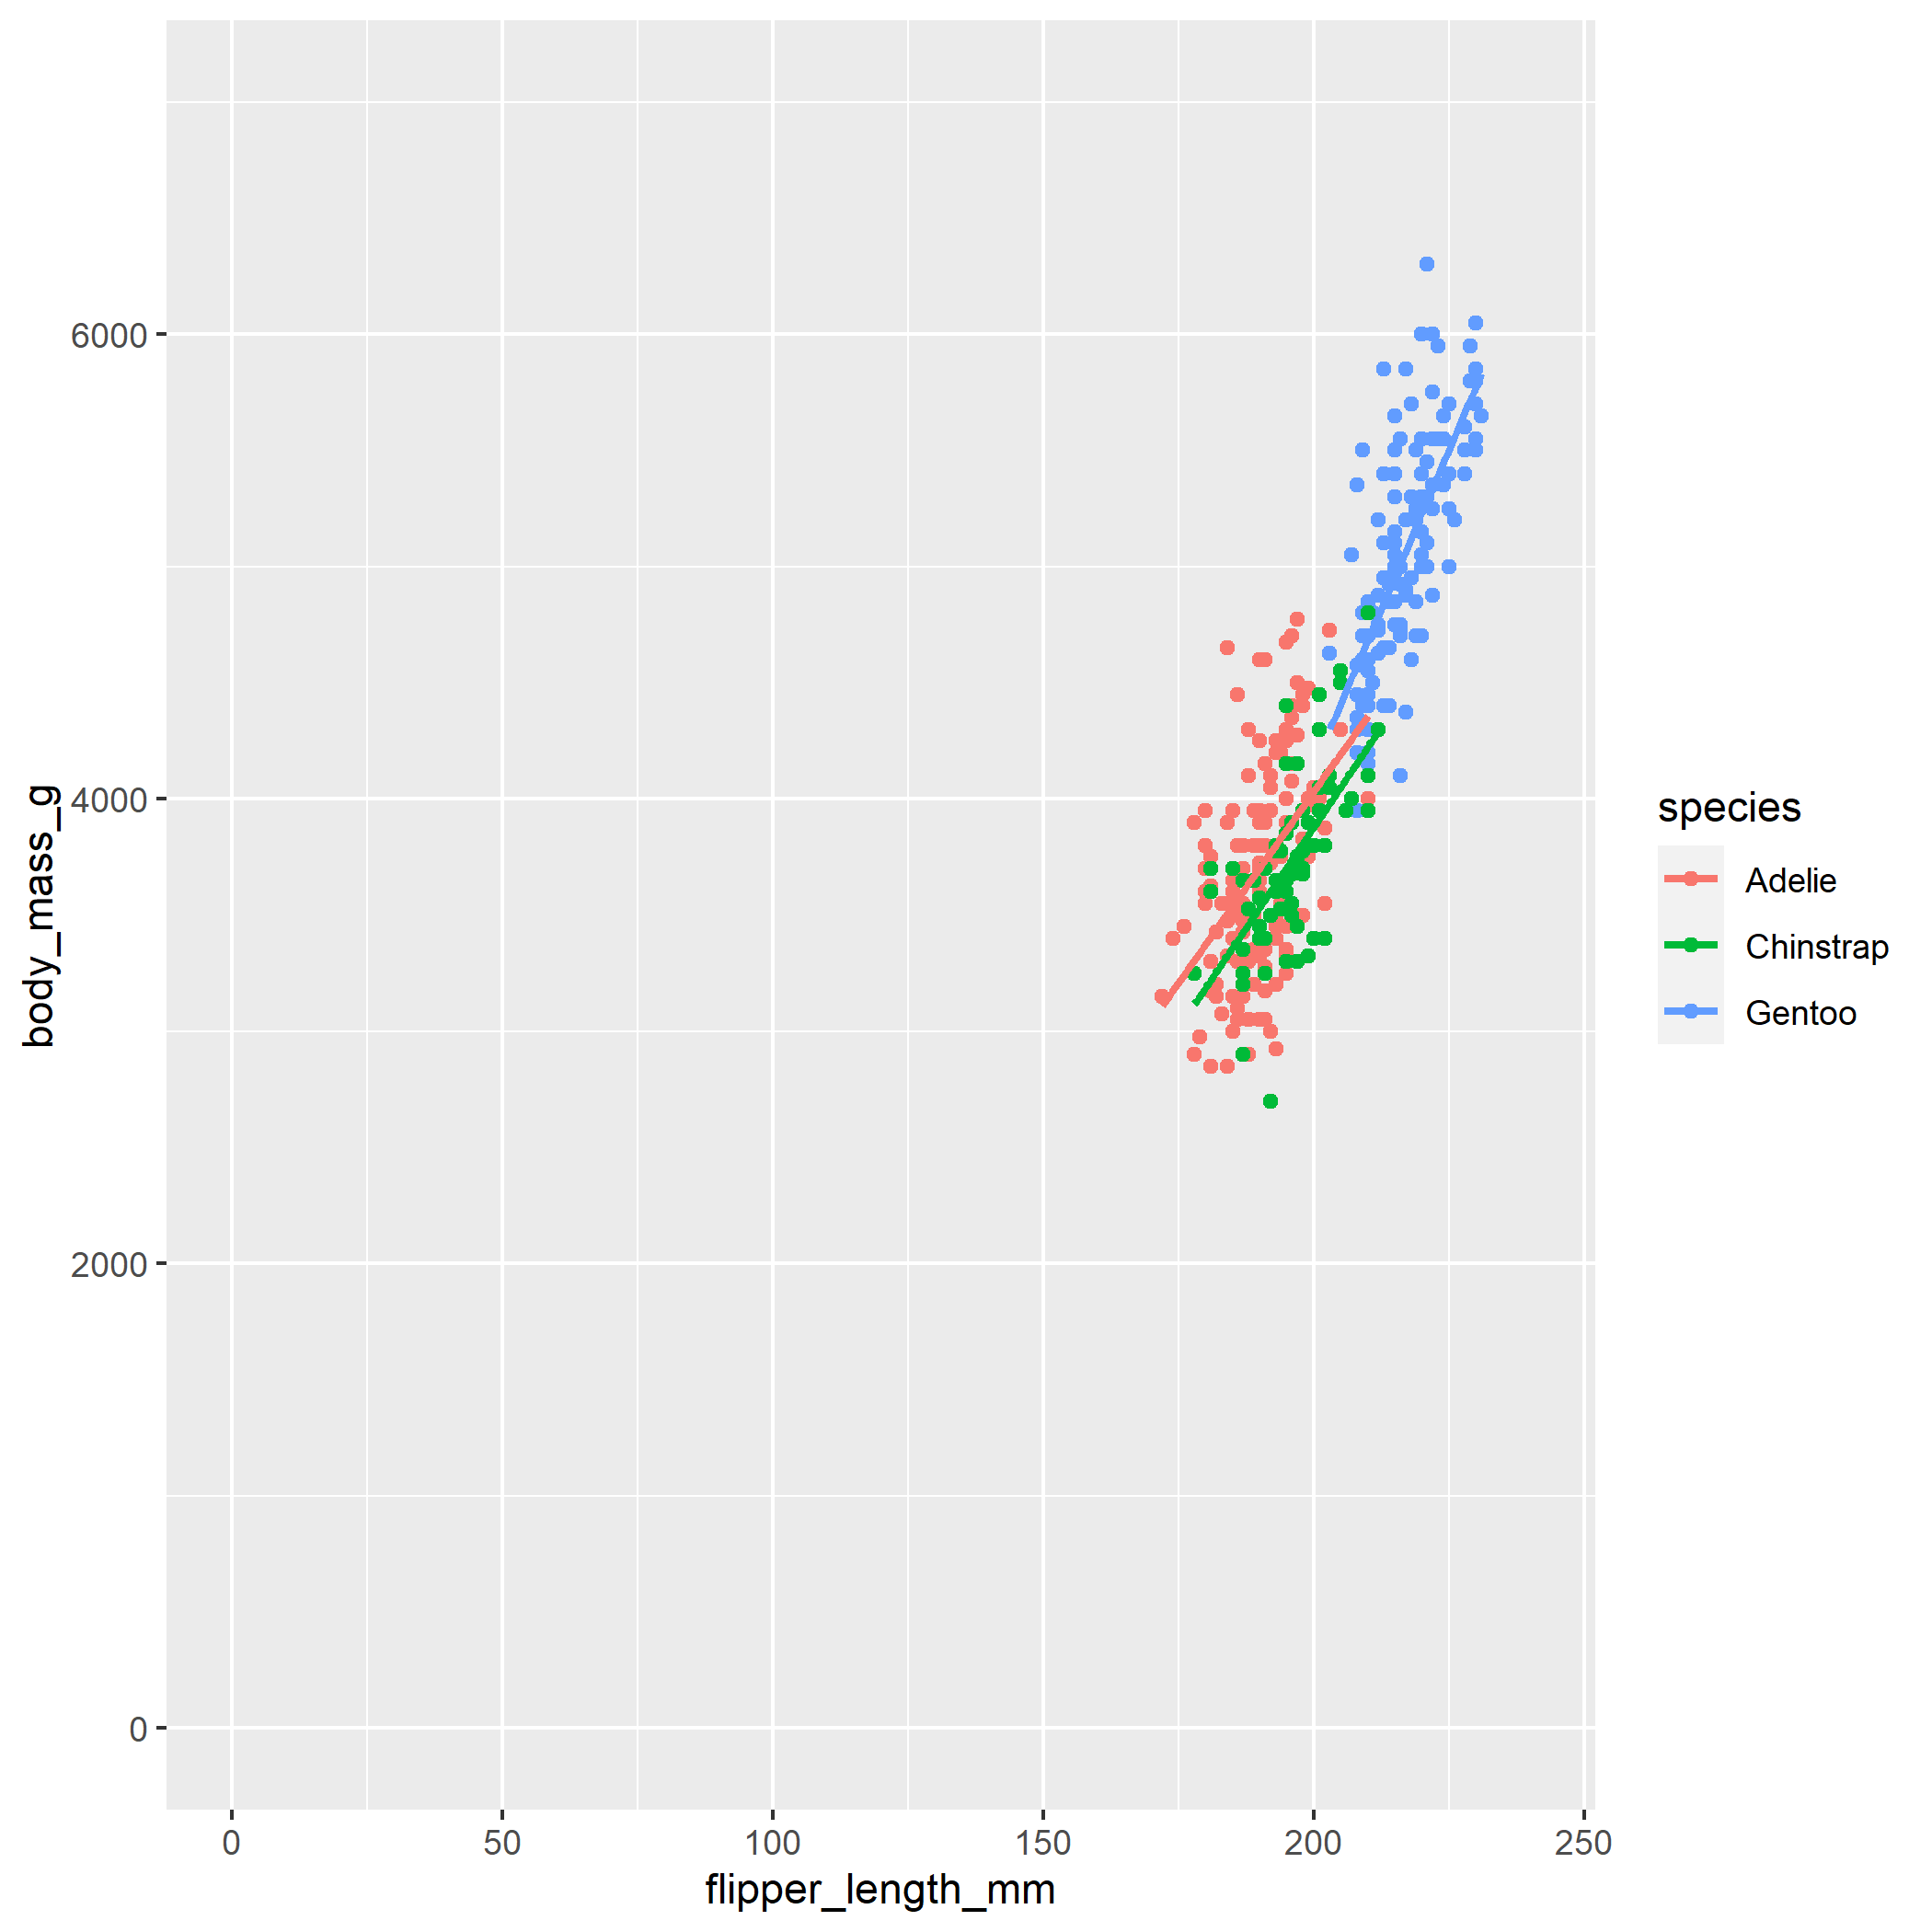
\includegraphics[width=0.8\linewidth]{images/zerolim}

Further, we can control the coordinate space using coord() functions. Say we want to flip the x and y axes, we add coord\_flip():

\begin{Shaded}
\begin{Highlighting}[]
\NormalTok{penguins }\SpecialCharTok{\%\textgreater{}\%} 
  \FunctionTok{ggplot}\NormalTok{(}\FunctionTok{aes}\NormalTok{(}\AttributeTok{x=}\NormalTok{flipper\_length\_mm, }
             \AttributeTok{y =}\NormalTok{ body\_mass\_g,}
             \AttributeTok{colour=}\NormalTok{species))}\SpecialCharTok{+} 
  \FunctionTok{geom\_point}\NormalTok{()}\SpecialCharTok{+}
  \FunctionTok{geom\_smooth}\NormalTok{(}\AttributeTok{method=}\StringTok{"lm"}\NormalTok{,    }
              \AttributeTok{se=}\ConstantTok{FALSE}\NormalTok{)}\SpecialCharTok{+}
  \FunctionTok{xlim}\NormalTok{(}\DecValTok{0}\NormalTok{,}\DecValTok{240}\NormalTok{) }\SpecialCharTok{+} \FunctionTok{ylim}\NormalTok{(}\DecValTok{0}\NormalTok{,}\DecValTok{7000}\NormalTok{)}\SpecialCharTok{+}
  \FunctionTok{coord\_flip}\NormalTok{()}
\end{Highlighting}
\end{Shaded}

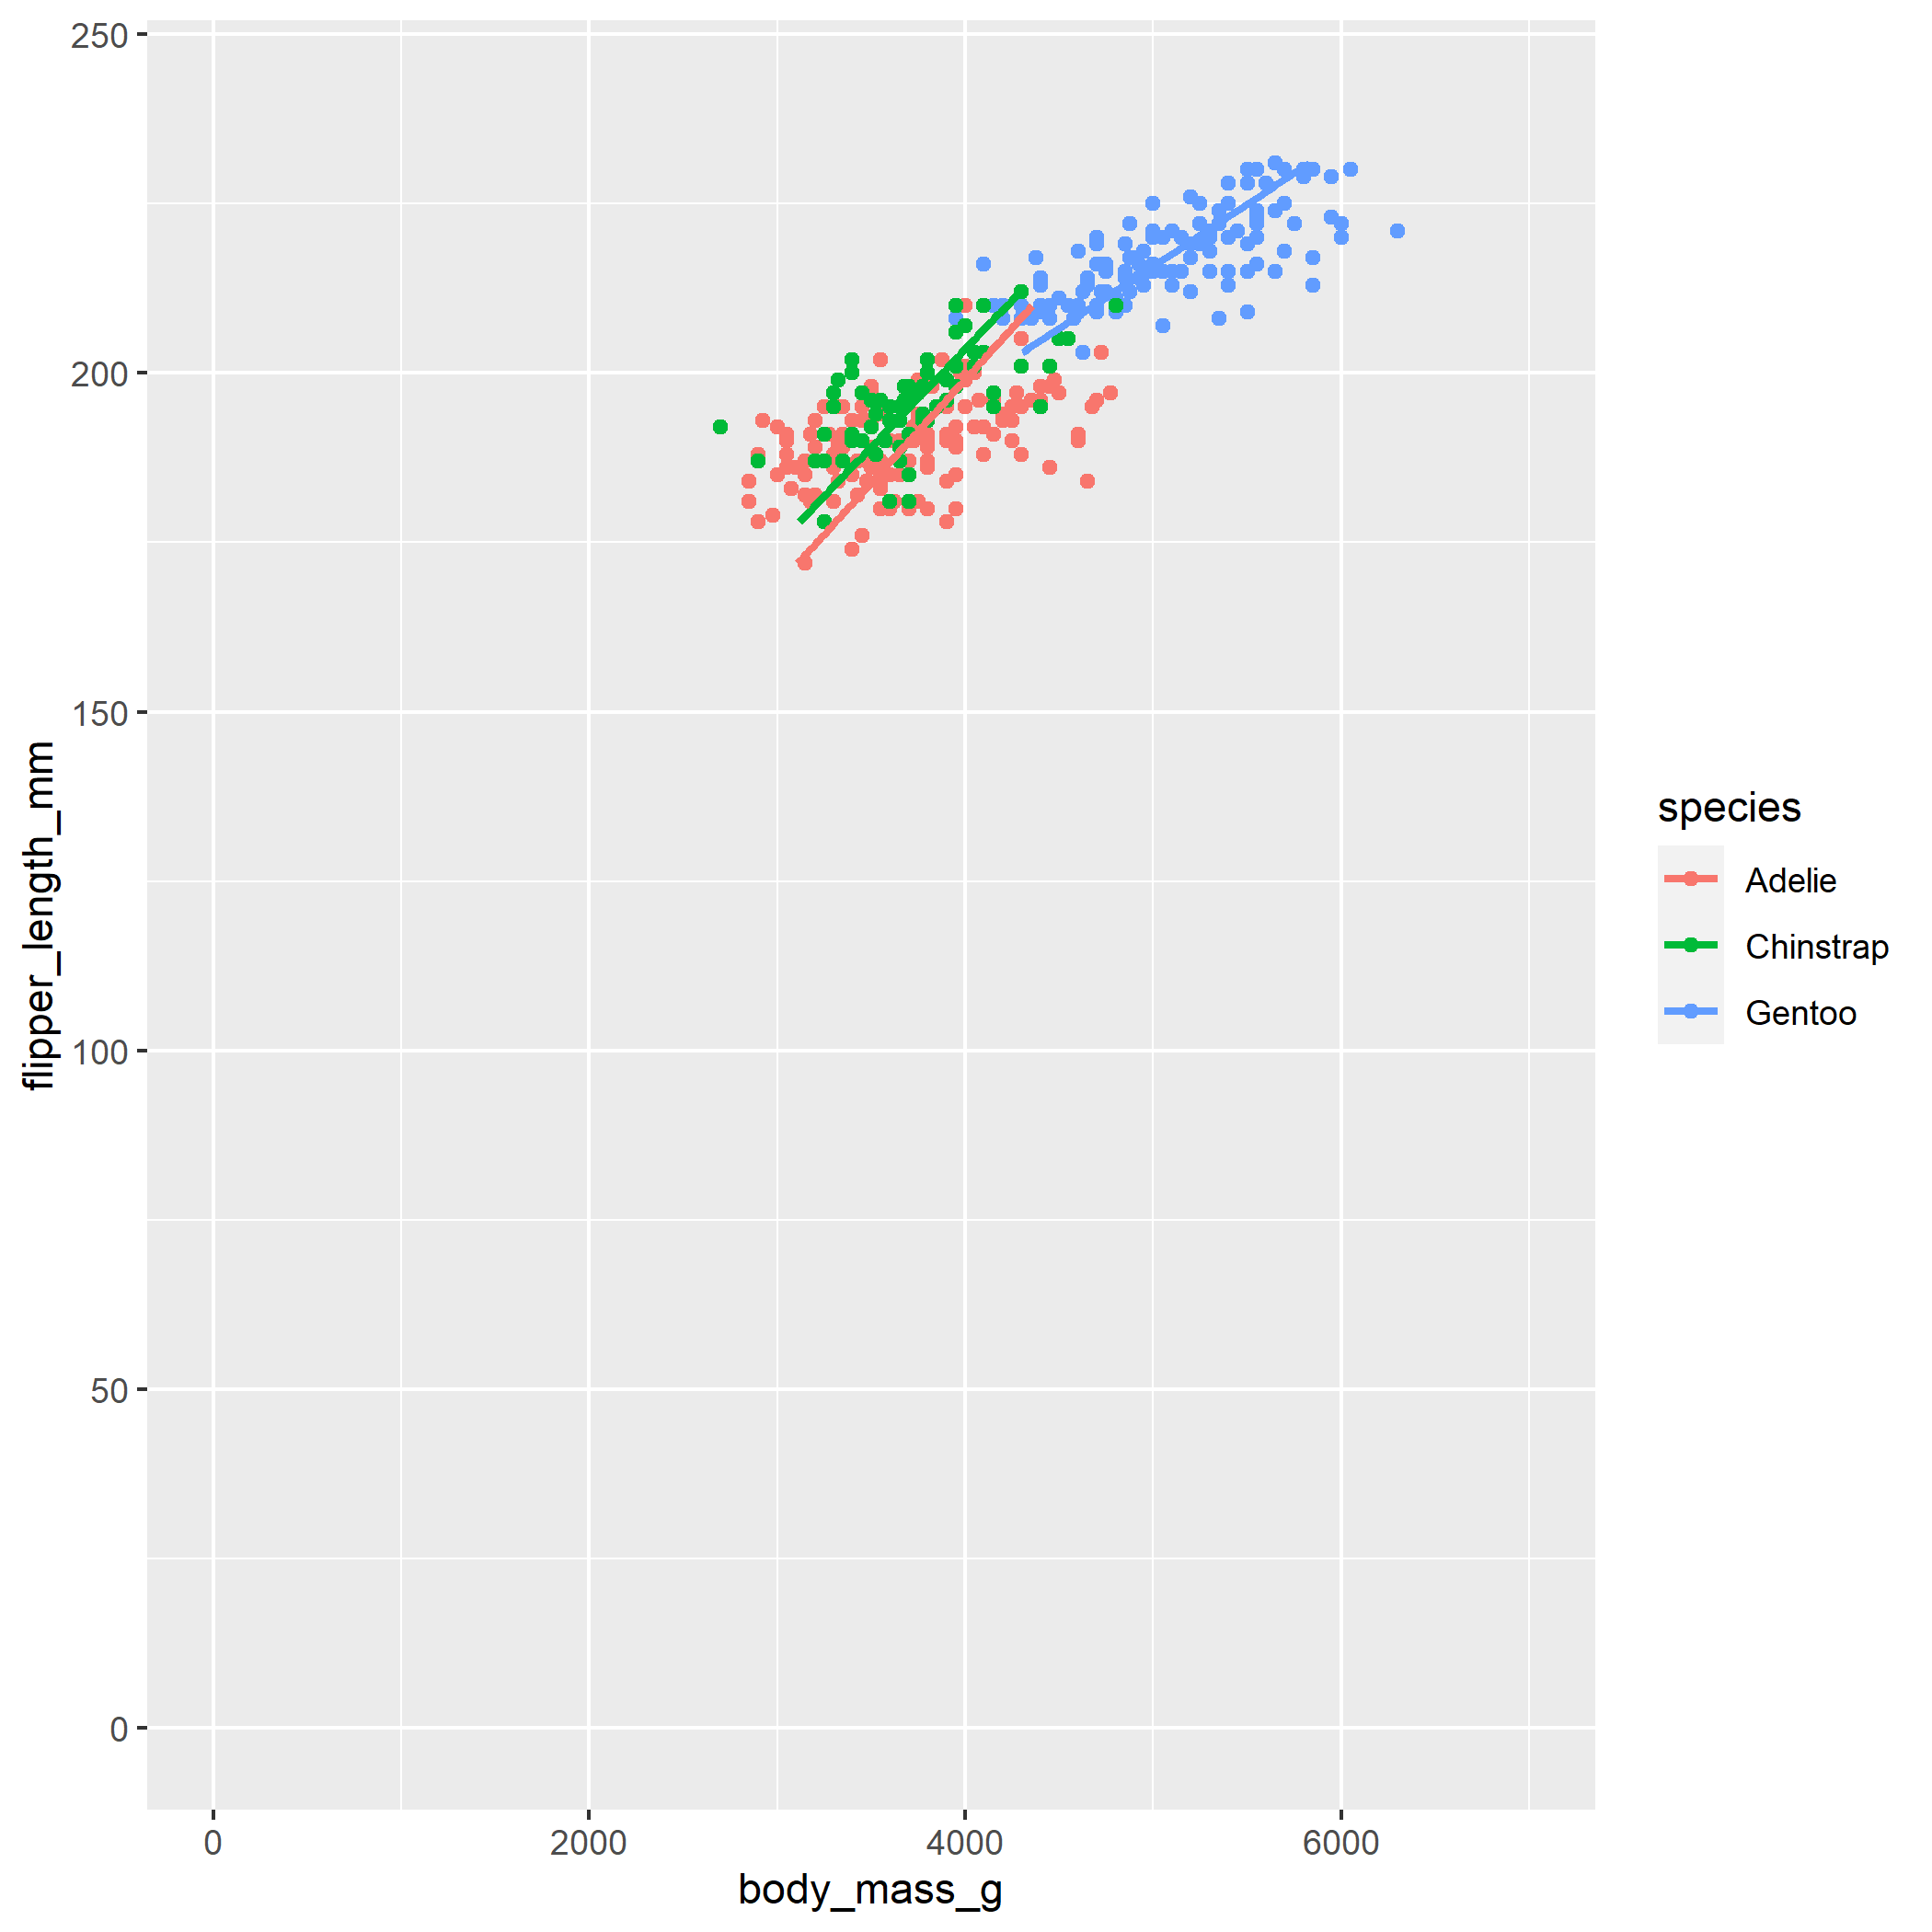
\includegraphics[width=0.8\linewidth]{images/flip}

\hypertarget{labels}{%
\section{Labels}\label{labels}}

By default, the axis labels will be the column names we gave as aesthetics aes(). We can change the axis labels using the xlab() and ylab() functions. Given that column names are often short and can be cryptic, this functionality is particularly important for effectively communicating results.

\begin{Shaded}
\begin{Highlighting}[]
\NormalTok{penguins }\SpecialCharTok{\%\textgreater{}\%} 
  \FunctionTok{ggplot}\NormalTok{(}\FunctionTok{aes}\NormalTok{(}\AttributeTok{x=}\NormalTok{flipper\_length\_mm, }
             \AttributeTok{y =}\NormalTok{ body\_mass\_g,}
             \AttributeTok{colour=}\NormalTok{species))}\SpecialCharTok{+} 
  \FunctionTok{geom\_point}\NormalTok{()}\SpecialCharTok{+}
  \FunctionTok{geom\_smooth}\NormalTok{(}\AttributeTok{method=}\StringTok{"lm"}\NormalTok{,    }
              \AttributeTok{se=}\ConstantTok{FALSE}\NormalTok{)}\SpecialCharTok{+}
  \FunctionTok{labs}\NormalTok{(}\AttributeTok{x =} \StringTok{"Flipper length (mm)"}\NormalTok{,}
       \AttributeTok{y =} \StringTok{"Body mass (g)"}\NormalTok{)}
\end{Highlighting}
\end{Shaded}

We can also add titles and subtitles

\begin{Shaded}
\begin{Highlighting}[]
\NormalTok{penguins }\SpecialCharTok{\%\textgreater{}\%} 
  \FunctionTok{ggplot}\NormalTok{(}\FunctionTok{aes}\NormalTok{(}\AttributeTok{x=}\NormalTok{flipper\_length\_mm, }
             \AttributeTok{y =}\NormalTok{ body\_mass\_g,}
             \AttributeTok{colour=}\NormalTok{species))}\SpecialCharTok{+} 
  \FunctionTok{geom\_point}\NormalTok{()}\SpecialCharTok{+}
  \FunctionTok{geom\_smooth}\NormalTok{(}\AttributeTok{method=}\StringTok{"lm"}\NormalTok{,    }
              \AttributeTok{se=}\ConstantTok{FALSE}\NormalTok{)}\SpecialCharTok{+}
  \FunctionTok{labs}\NormalTok{(}\AttributeTok{x =} \StringTok{"Flipper length (mm)"}\NormalTok{,}
       \AttributeTok{y =} \StringTok{"Body mass (g)"}\NormalTok{,}
       \AttributeTok{title=} \StringTok{"Penguin Size, Palmer Station LTER"}\NormalTok{,}
       \AttributeTok{subtitle=} \StringTok{"Flipper length and body mass for Adelie, Chinstrap and Gentoo penguins"}\NormalTok{)}
\end{Highlighting}
\end{Shaded}

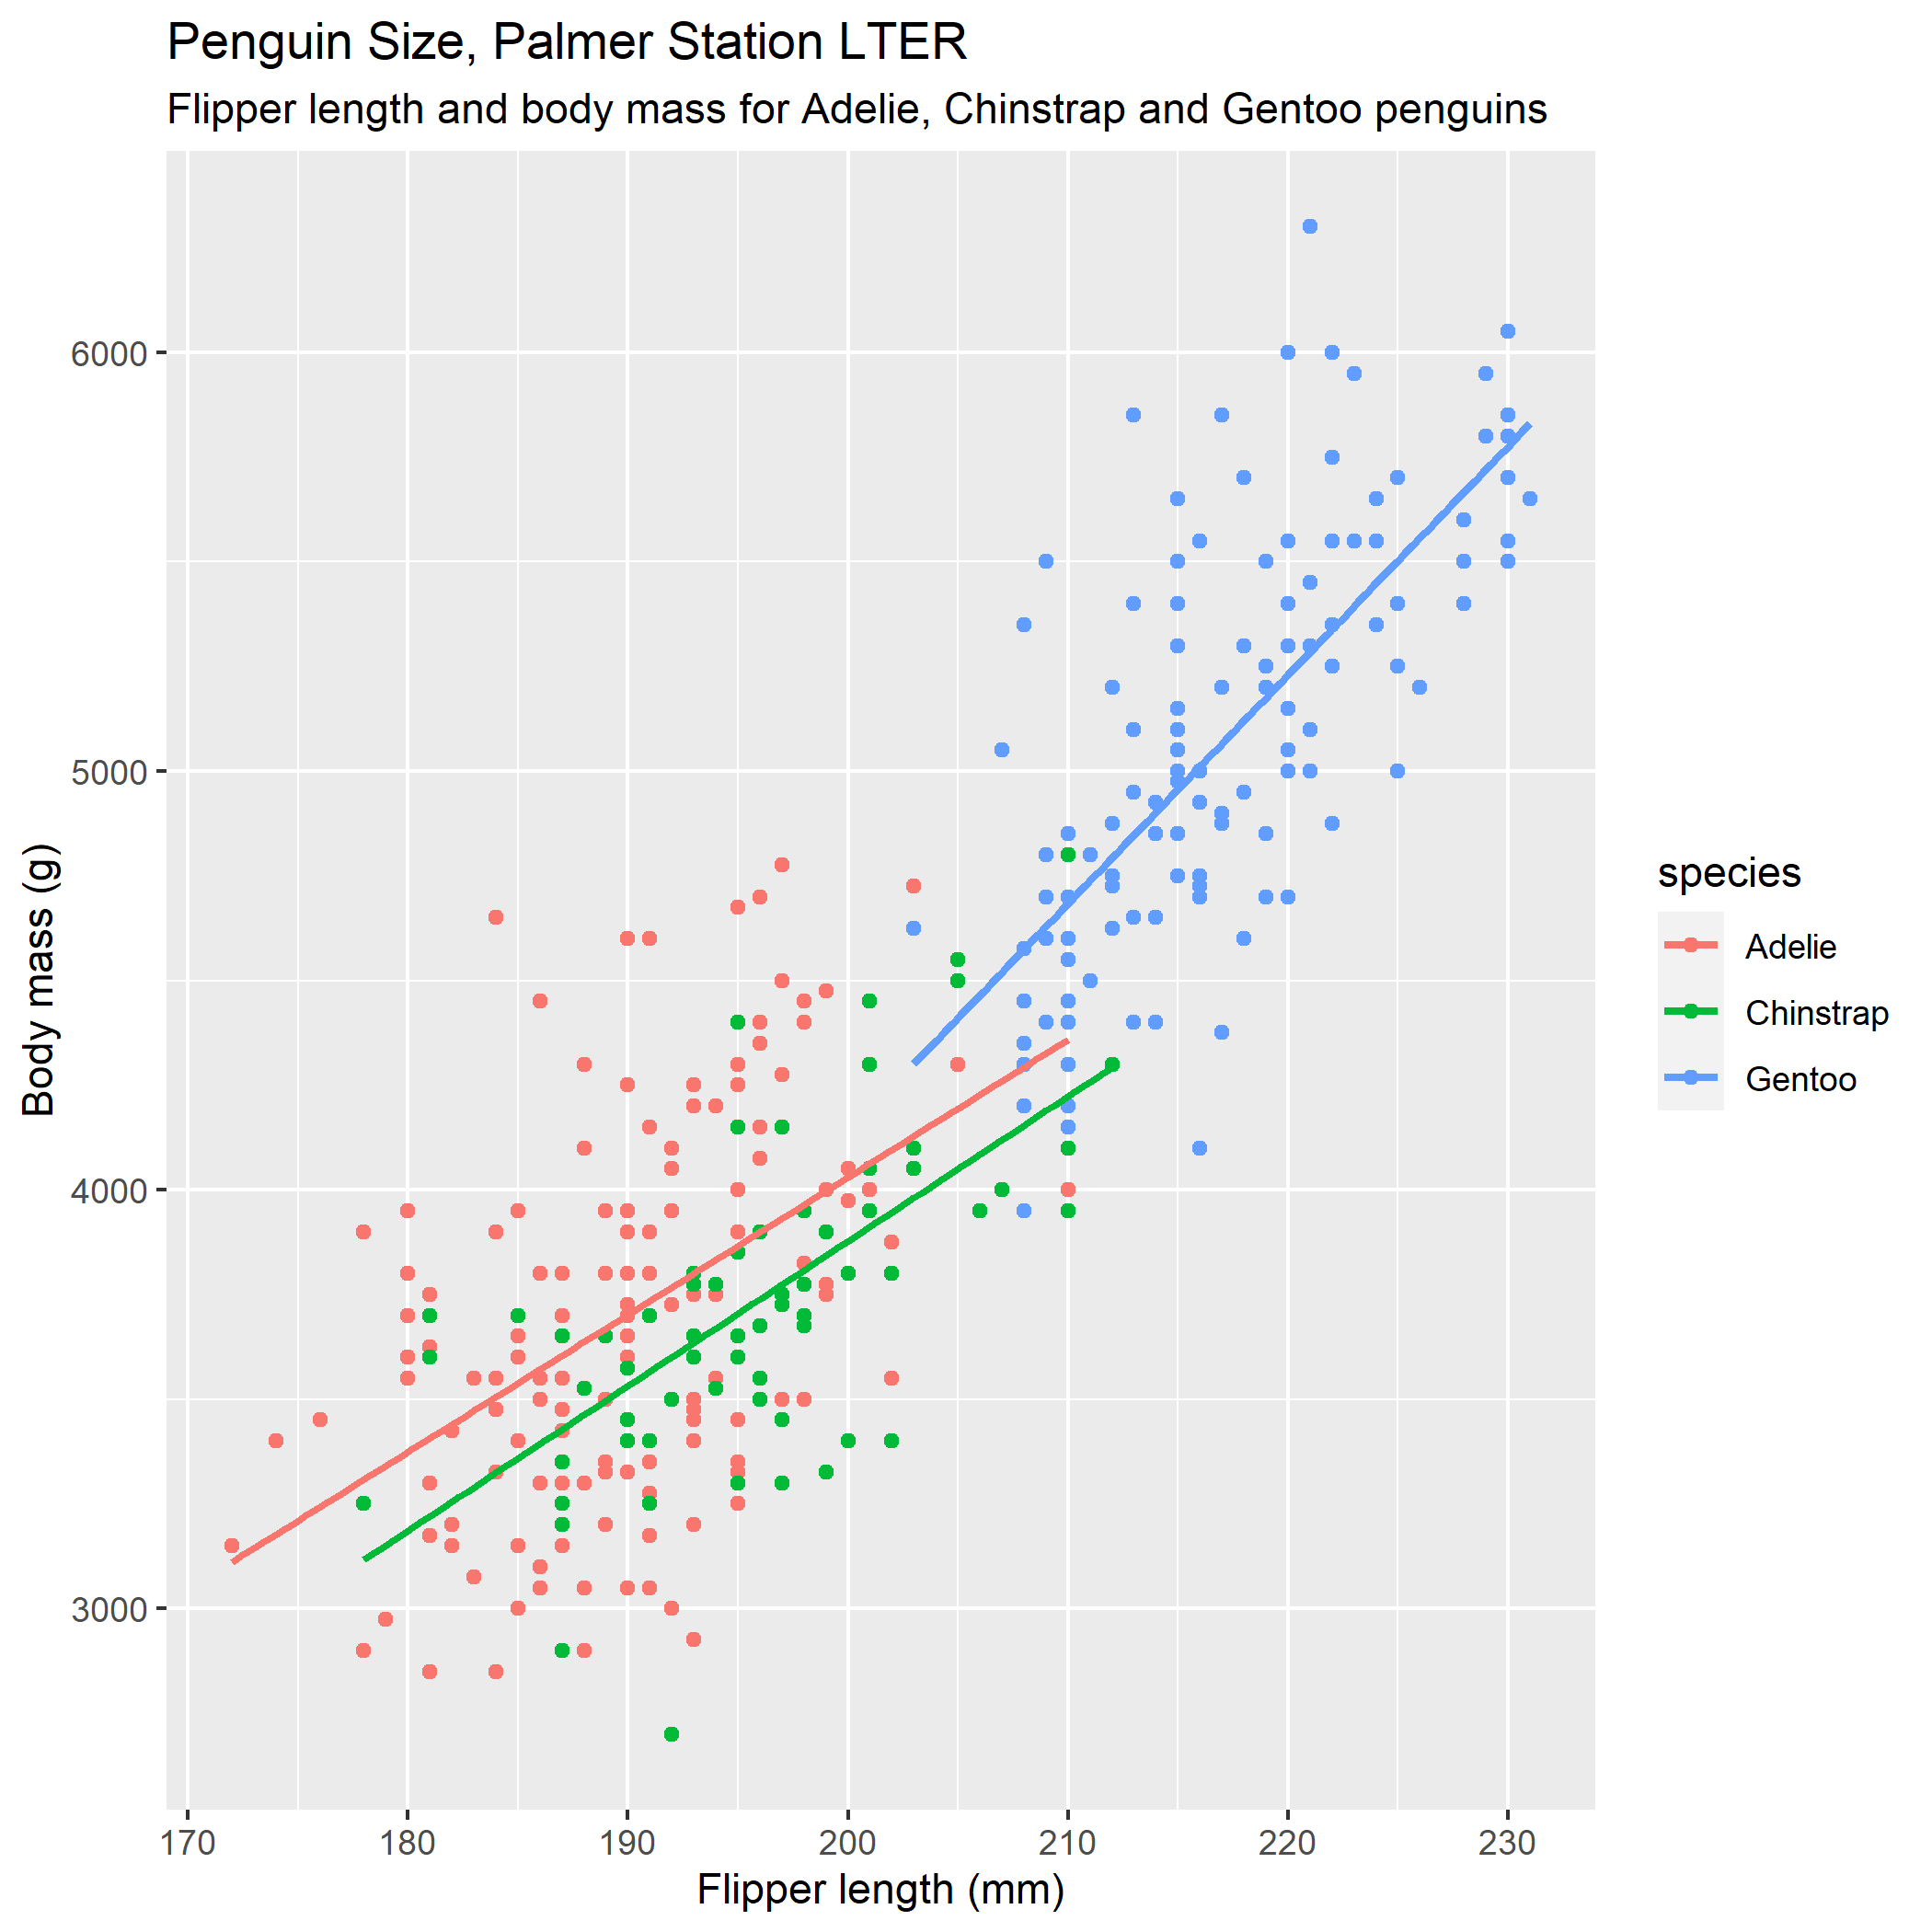
\includegraphics[width=0.8\linewidth]{images/title}

\hypertarget{themes}{%
\section{Themes}\label{themes}}

Finally, the overall appearance of the plot can be modified using theme() functions. The default theme has a grey background which maximizes contrast with other contrasts.
You may prefer \texttt{theme\_classic()}, a \texttt{theme\_minimal()} or even \texttt{theme\_void()}. Try them out.

\begin{Shaded}
\begin{Highlighting}[]
\NormalTok{penguins }\SpecialCharTok{\%\textgreater{}\%} 
  \FunctionTok{ggplot}\NormalTok{(}\FunctionTok{aes}\NormalTok{(}\AttributeTok{x=}\NormalTok{flipper\_length\_mm, }
             \AttributeTok{y =}\NormalTok{ body\_mass\_g,}
             \AttributeTok{colour=}\NormalTok{species))}\SpecialCharTok{+} 
  \FunctionTok{geom\_point}\NormalTok{()}\SpecialCharTok{+}
  \FunctionTok{geom\_smooth}\NormalTok{(}\AttributeTok{method=}\StringTok{"lm"}\NormalTok{,    }
              \AttributeTok{se=}\ConstantTok{FALSE}\NormalTok{)}\SpecialCharTok{+}
  \FunctionTok{labs}\NormalTok{(}\AttributeTok{x =} \StringTok{"Flipper length (mm)"}\NormalTok{,}
       \AttributeTok{y =} \StringTok{"Body mass (g)"}\NormalTok{,}
       \AttributeTok{title=} \StringTok{"Penguin Size, Palmer Station LTER"}\NormalTok{,}
       \AttributeTok{subtitle=} \StringTok{"Flipper length and body mass for Adelie, Chinstrap and Gentoo penguins"}\NormalTok{)}\SpecialCharTok{+}
  \FunctionTok{theme\_bw}\NormalTok{()}
\end{Highlighting}
\end{Shaded}

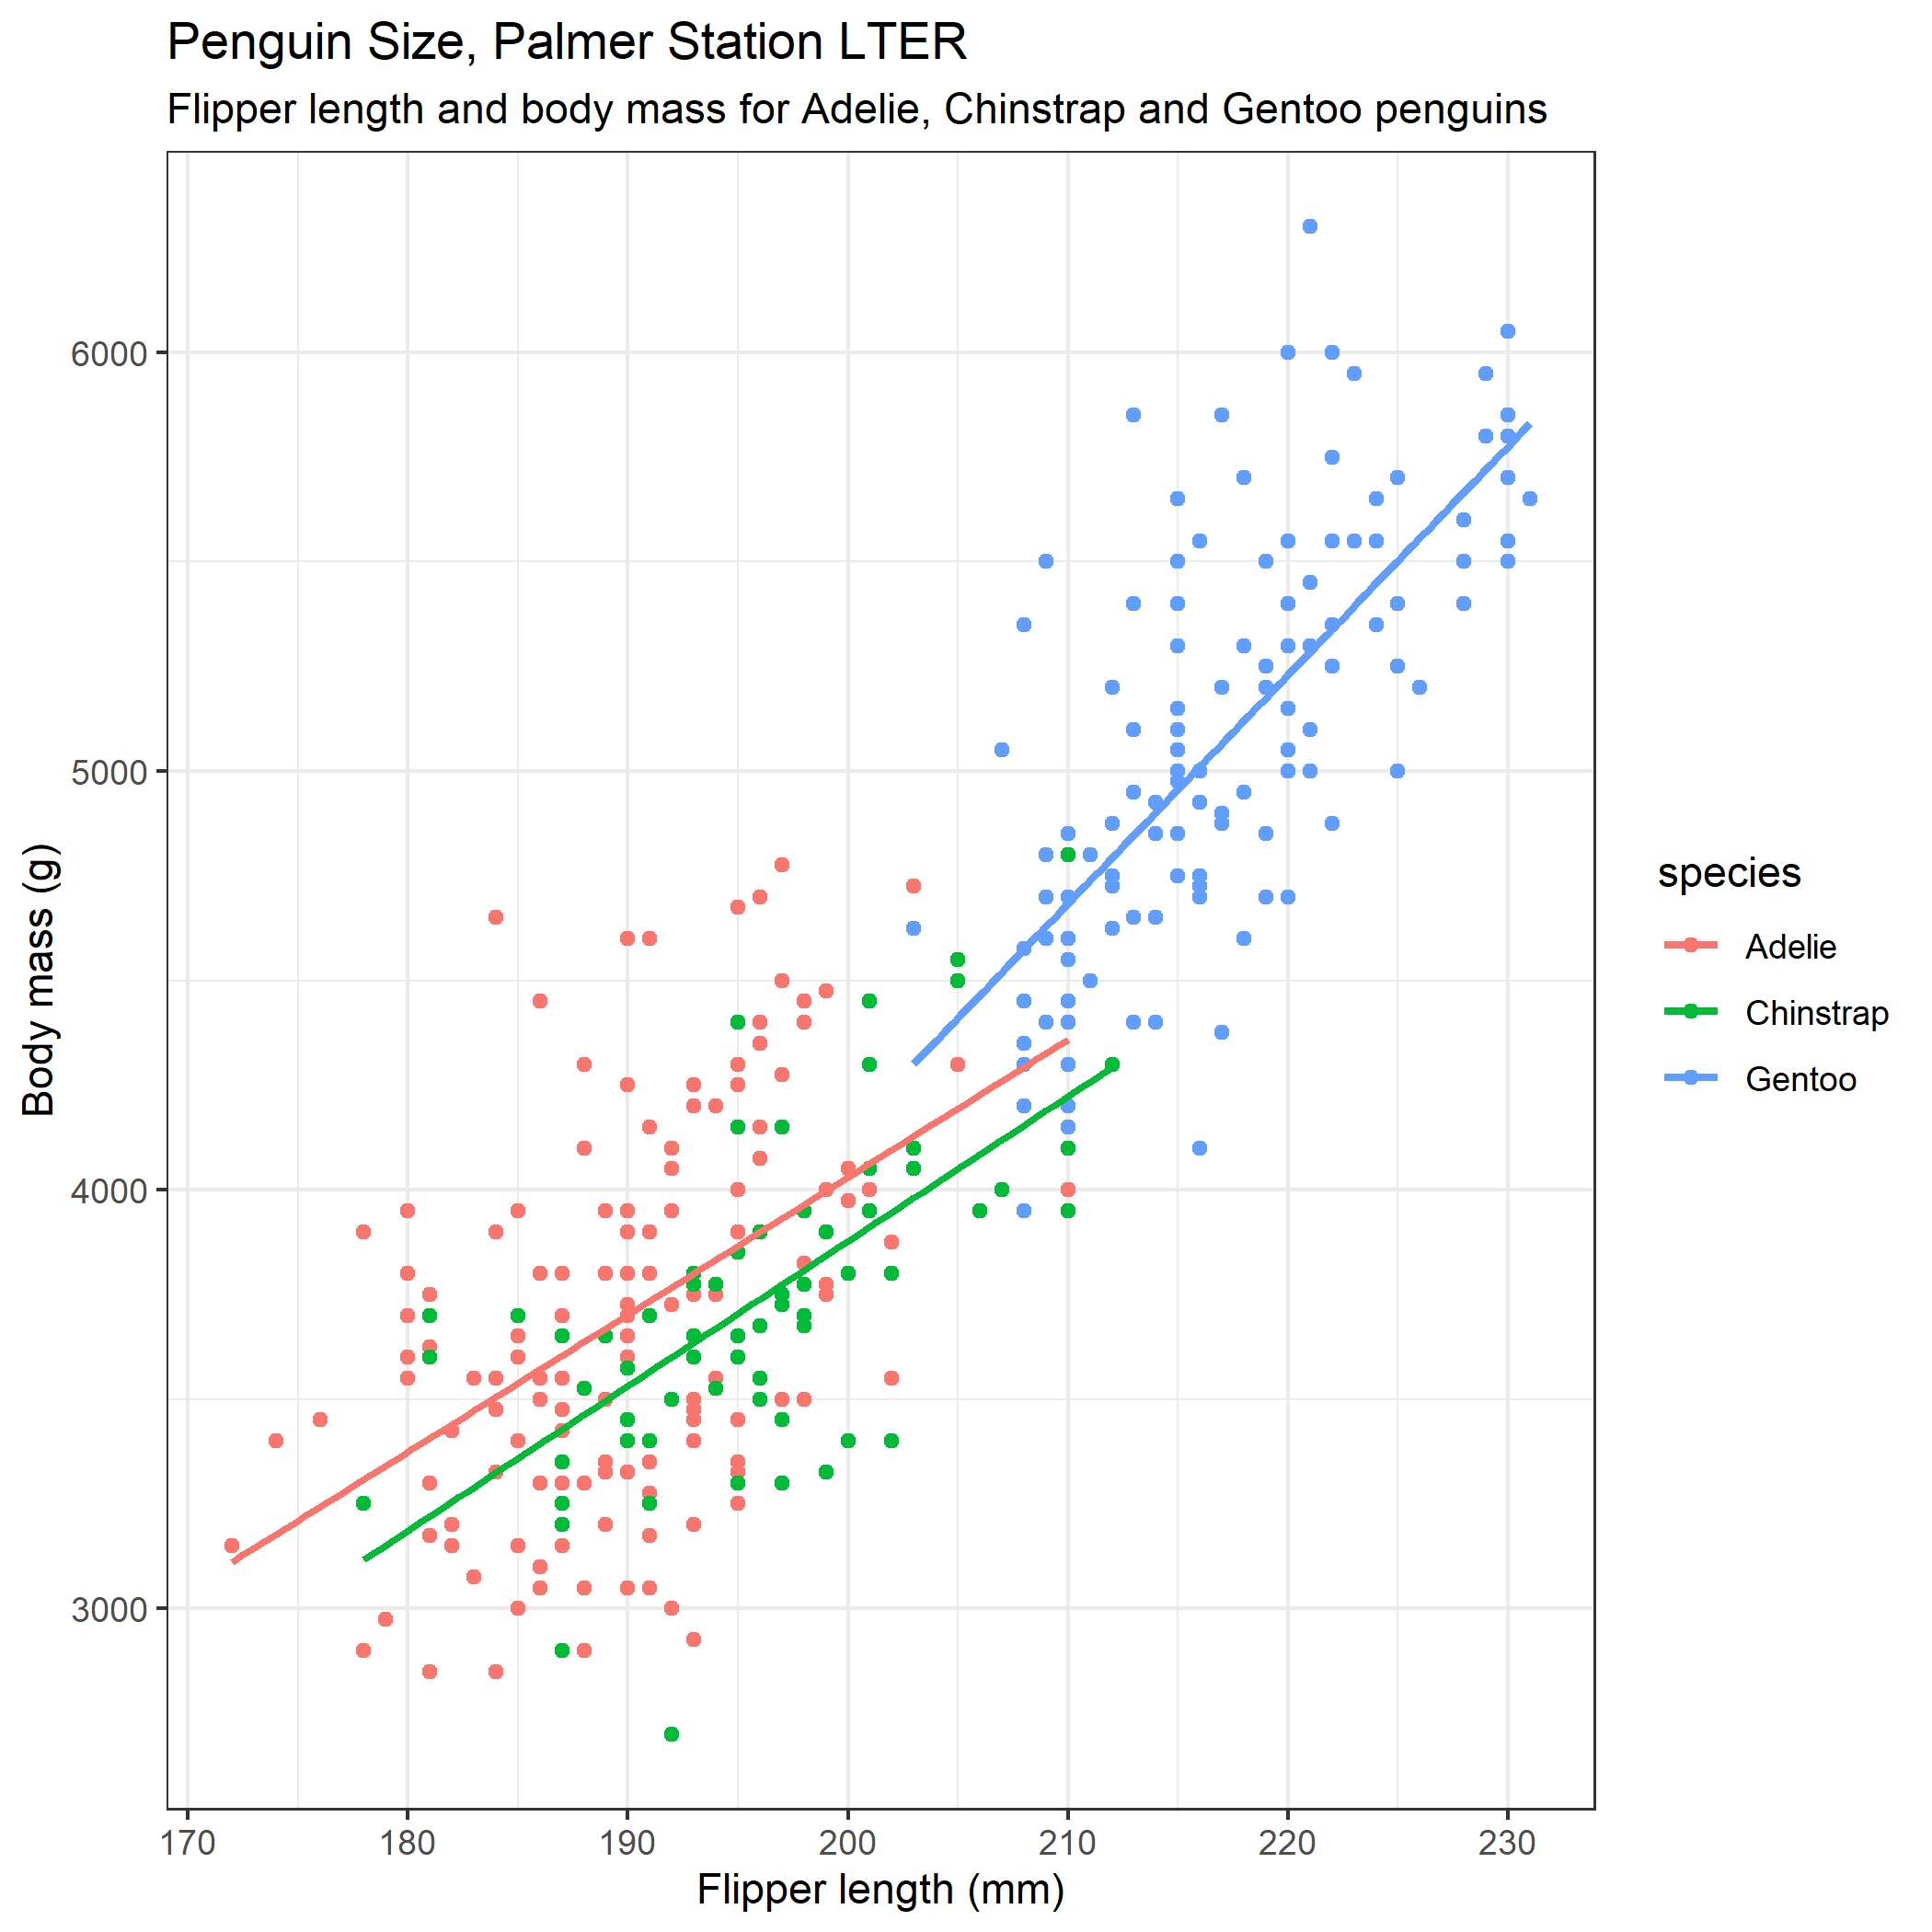
\includegraphics[width=0.8\linewidth]{images/theme_bw}

\begin{quote}
**Note - there is a lot more customisation available through the theme() function. We will look at making our own custom themes in later lessons
\end{quote}

\begin{rmdwarning}
You can try installing and running an even wider range of pre-built
themes if you install the R package \texttt{ggthemes}.

First you will need to run the \texttt{install.packages("ggthemes")}
command. Remember this is one of the few times a command should NOT be
written in your script but typed directly into the console. That's
because it's rude to send someone a script that will install packages on
their computer - think of library() as a polite request instead!

To access the range of themes available type \texttt{help(ggthemes)}
then follow the documentation to find out what you can do.
\end{rmdwarning}

\hypertarget{jitter}{%
\section{Jitter}\label{jitter}}

The geom\_jitter() command adds some random scatter to the points which can reduce over-plotting. Compare these two plots:

\begin{Shaded}
\begin{Highlighting}[]
\FunctionTok{ggplot}\NormalTok{(}\AttributeTok{data =}\NormalTok{ penguins, }\FunctionTok{aes}\NormalTok{(}\AttributeTok{x =}\NormalTok{ species, }\AttributeTok{y =}\NormalTok{ bill\_length\_mm)) }\SpecialCharTok{+}
  \FunctionTok{geom\_jitter}\NormalTok{(}\FunctionTok{aes}\NormalTok{(}\AttributeTok{color =}\NormalTok{ species),}
              \AttributeTok{width =} \FloatTok{0.1}\NormalTok{, }\CommentTok{\# specifies the width, change this to change the range of scatter}
              \AttributeTok{alpha =} \FloatTok{0.7}\NormalTok{, }\CommentTok{\# specifies the amount of transparency in the points}
              \AttributeTok{show.legend =} \ConstantTok{FALSE}\NormalTok{) }\CommentTok{\# don\textquotesingle{}t leave a legend in a plot, if it doesn\textquotesingle{}t add value}
\end{Highlighting}
\end{Shaded}

\begin{Shaded}
\begin{Highlighting}[]
\FunctionTok{ggplot}\NormalTok{(}\AttributeTok{data =}\NormalTok{ penguins, }\FunctionTok{aes}\NormalTok{(}\AttributeTok{x =}\NormalTok{ species, }\AttributeTok{y =}\NormalTok{ bill\_length\_mm)) }\SpecialCharTok{+}
  \FunctionTok{geom\_point}\NormalTok{(}\FunctionTok{aes}\NormalTok{(}\AttributeTok{color =}\NormalTok{ species),}
              \AttributeTok{alpha =} \FloatTok{0.7}\NormalTok{, }
              \AttributeTok{show.legend =} \ConstantTok{FALSE}\NormalTok{) }
\end{Highlighting}
\end{Shaded}

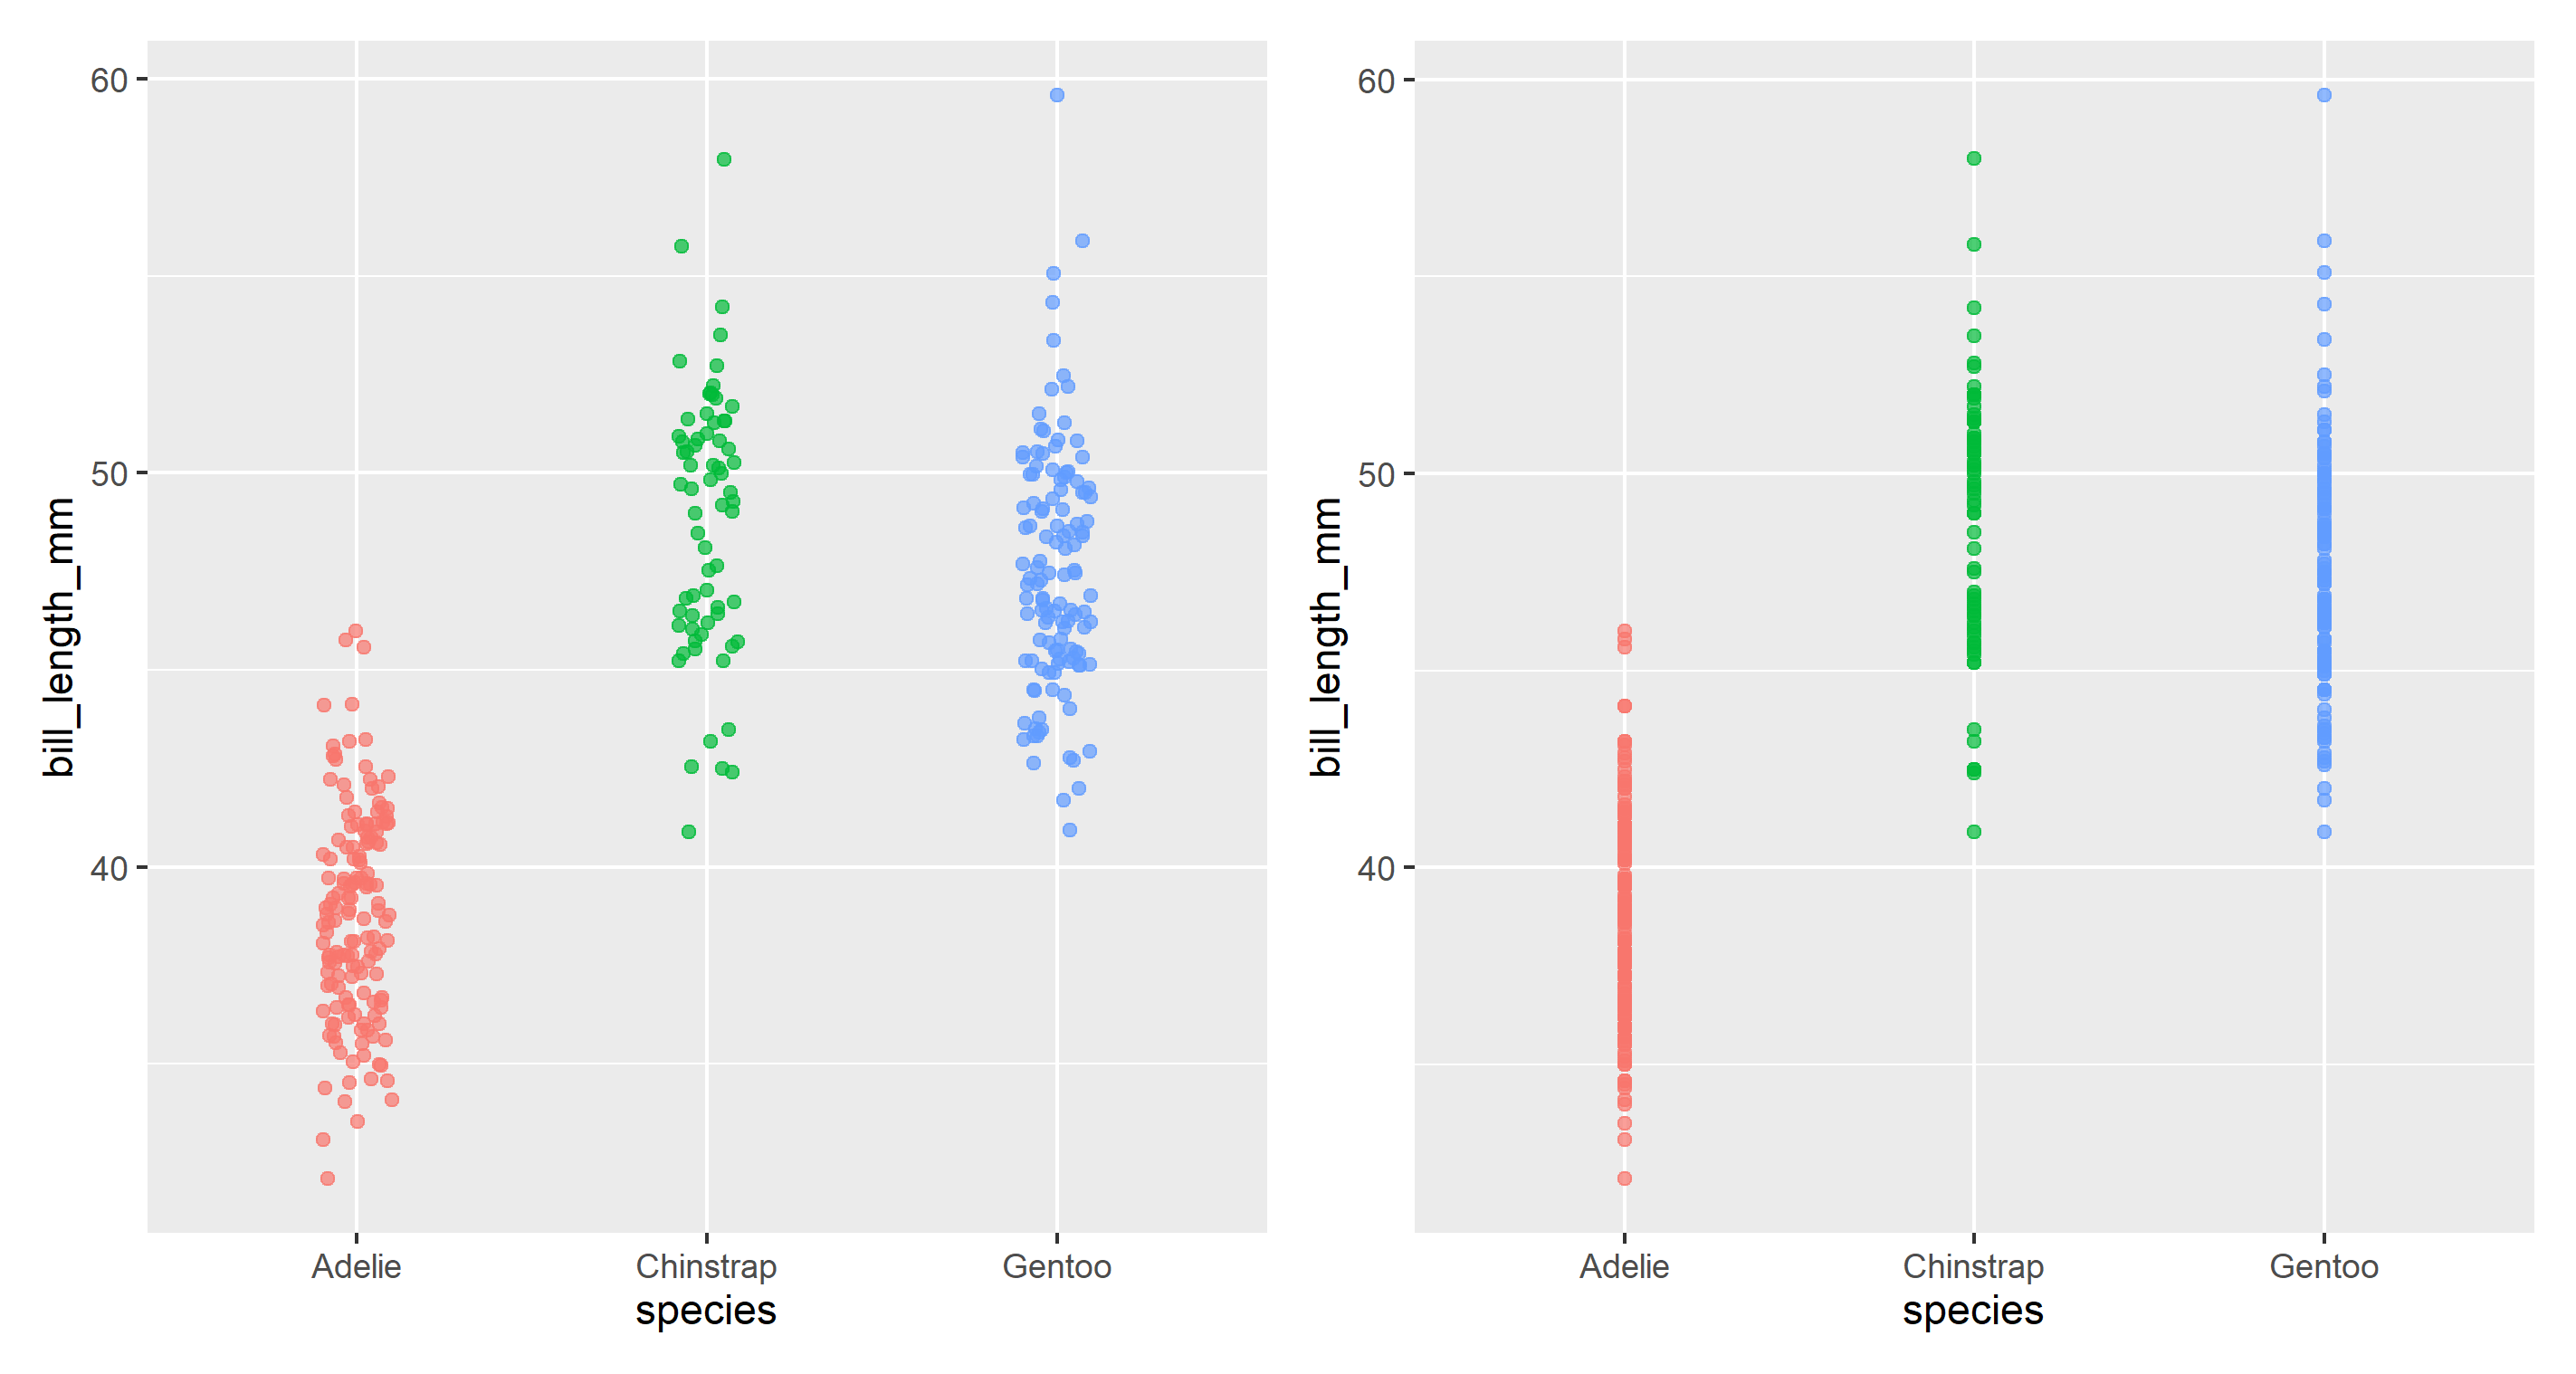
\includegraphics[width=0.8\linewidth]{images/jitter}

\hypertarget{boxplots}{%
\section{Boxplots}\label{boxplots}}

Box plots, or `box \& whisker plots' are another essential tool for data analysis. Box plots summarize the distribution of a set of values by displaying the minimum and maximum values, the median (i.e.~middle-ranked value), and the range of the middle 50\% of values (inter-quartile range).
The whisker line extending above and below the IQR box define Q3 + (1.5 x IQR), and Q1 - (1.5 x IQR) respectively. You can watch a short video to learn more about box plots \href{https://www.youtube.com/watch?v=fHLhBnmwUM0}{here}.

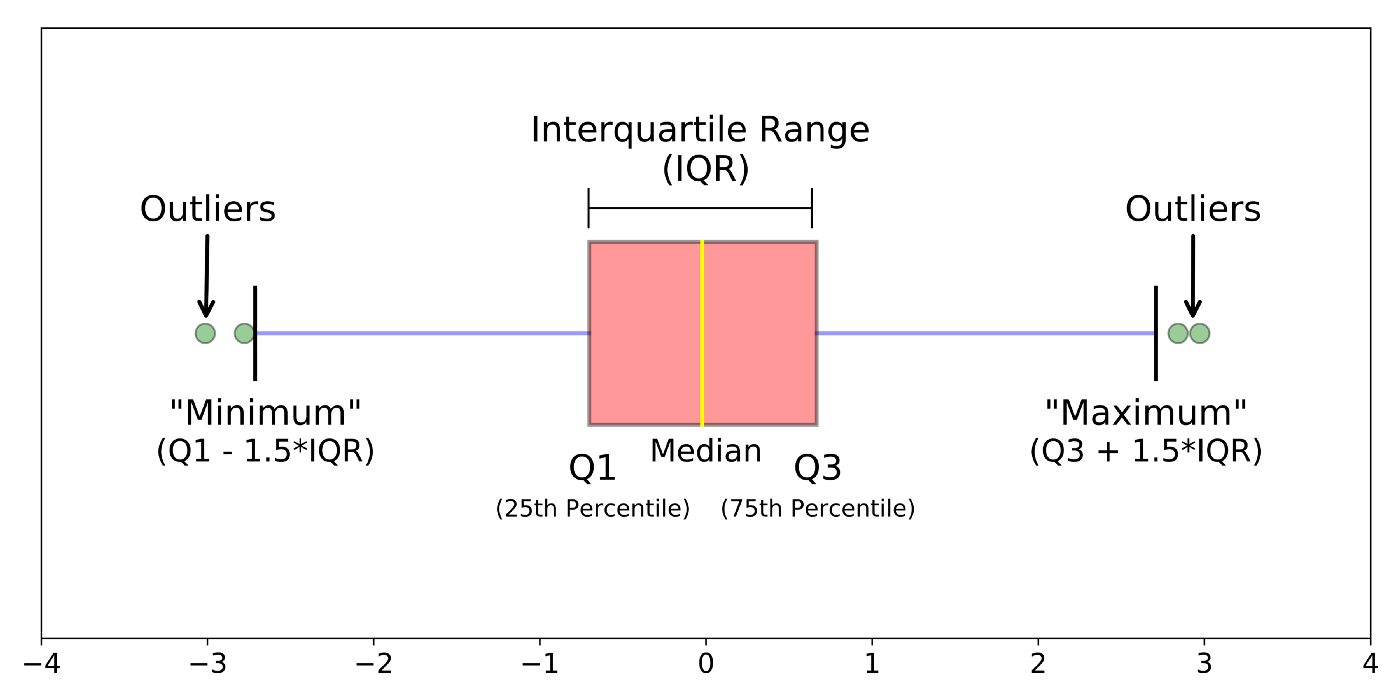
\includegraphics[width=0.8\linewidth]{images/boxplot}

To create a box plot from our data we use (no prizes here) geom\_boxplot()!

\begin{Shaded}
\begin{Highlighting}[]
\FunctionTok{ggplot}\NormalTok{(}\AttributeTok{data =}\NormalTok{ penguins, }\FunctionTok{aes}\NormalTok{(}\AttributeTok{x =}\NormalTok{ species, }\AttributeTok{y =}\NormalTok{ bill\_length\_mm)) }\SpecialCharTok{+}
  \FunctionTok{geom\_boxplot}\NormalTok{(}\FunctionTok{aes}\NormalTok{(}\AttributeTok{fill =}\NormalTok{ species), }\CommentTok{\# note fill is "inside" colour and colour is "edges" {-} try it for yourself}
              \AttributeTok{alpha =} \FloatTok{0.7}\NormalTok{, }
              \AttributeTok{width =} \FloatTok{0.5}\NormalTok{, }\CommentTok{\# change width of boxplot}
              \AttributeTok{show.legend =} \ConstantTok{FALSE}\NormalTok{)}
\end{Highlighting}
\end{Shaded}

The points indicate outlier values {[}i.e., those greater than Q3 + (1.5 x IQR){]}.

We can overlay a boxplot on the scatter plot for the entire dataset, to fully communicate both the raw and summary data. Here we reduce the width of the jitter points slightly.

\begin{Shaded}
\begin{Highlighting}[]
\FunctionTok{ggplot}\NormalTok{(}\AttributeTok{data =}\NormalTok{ penguins, }\FunctionTok{aes}\NormalTok{(}\AttributeTok{x =}\NormalTok{ species, }\AttributeTok{y =}\NormalTok{ bill\_length\_mm)) }\SpecialCharTok{+}
  \FunctionTok{geom\_boxplot}\NormalTok{(}\FunctionTok{aes}\NormalTok{(}\AttributeTok{fill =}\NormalTok{ species), }\CommentTok{\# note fill is "inside" colour and colour is "edges" {-} try it for yourself}
              \AttributeTok{alpha =} \FloatTok{0.2}\NormalTok{, }\CommentTok{\# fainter boxes so the points "pop"}
              \AttributeTok{width =} \FloatTok{0.5}\NormalTok{, }\CommentTok{\# change width of boxplot}
              \AttributeTok{outlier.shape=}\ConstantTok{NA}\NormalTok{)}\SpecialCharTok{+}
  \FunctionTok{geom\_jitter}\NormalTok{(}\FunctionTok{aes}\NormalTok{(}\AttributeTok{colour =}\NormalTok{ species),}
                \AttributeTok{width=}\FloatTok{0.2}\NormalTok{)}\SpecialCharTok{+}
  \FunctionTok{theme}\NormalTok{(}\AttributeTok{legend.position =} \StringTok{"none"}\NormalTok{)}
\end{Highlighting}
\end{Shaded}

\begin{rmdwarning}
In the above example I switched from using show.legend=FALSE inside the
geom layer to using theme(legend.position=``none''). Why? This is an
example of reducing redunant code. I would have to specify
show.legend=FALSE for every geom layer in my plot, but the theme
function applies to every layer. Save code, save time, reduce errors!
\end{rmdwarning}

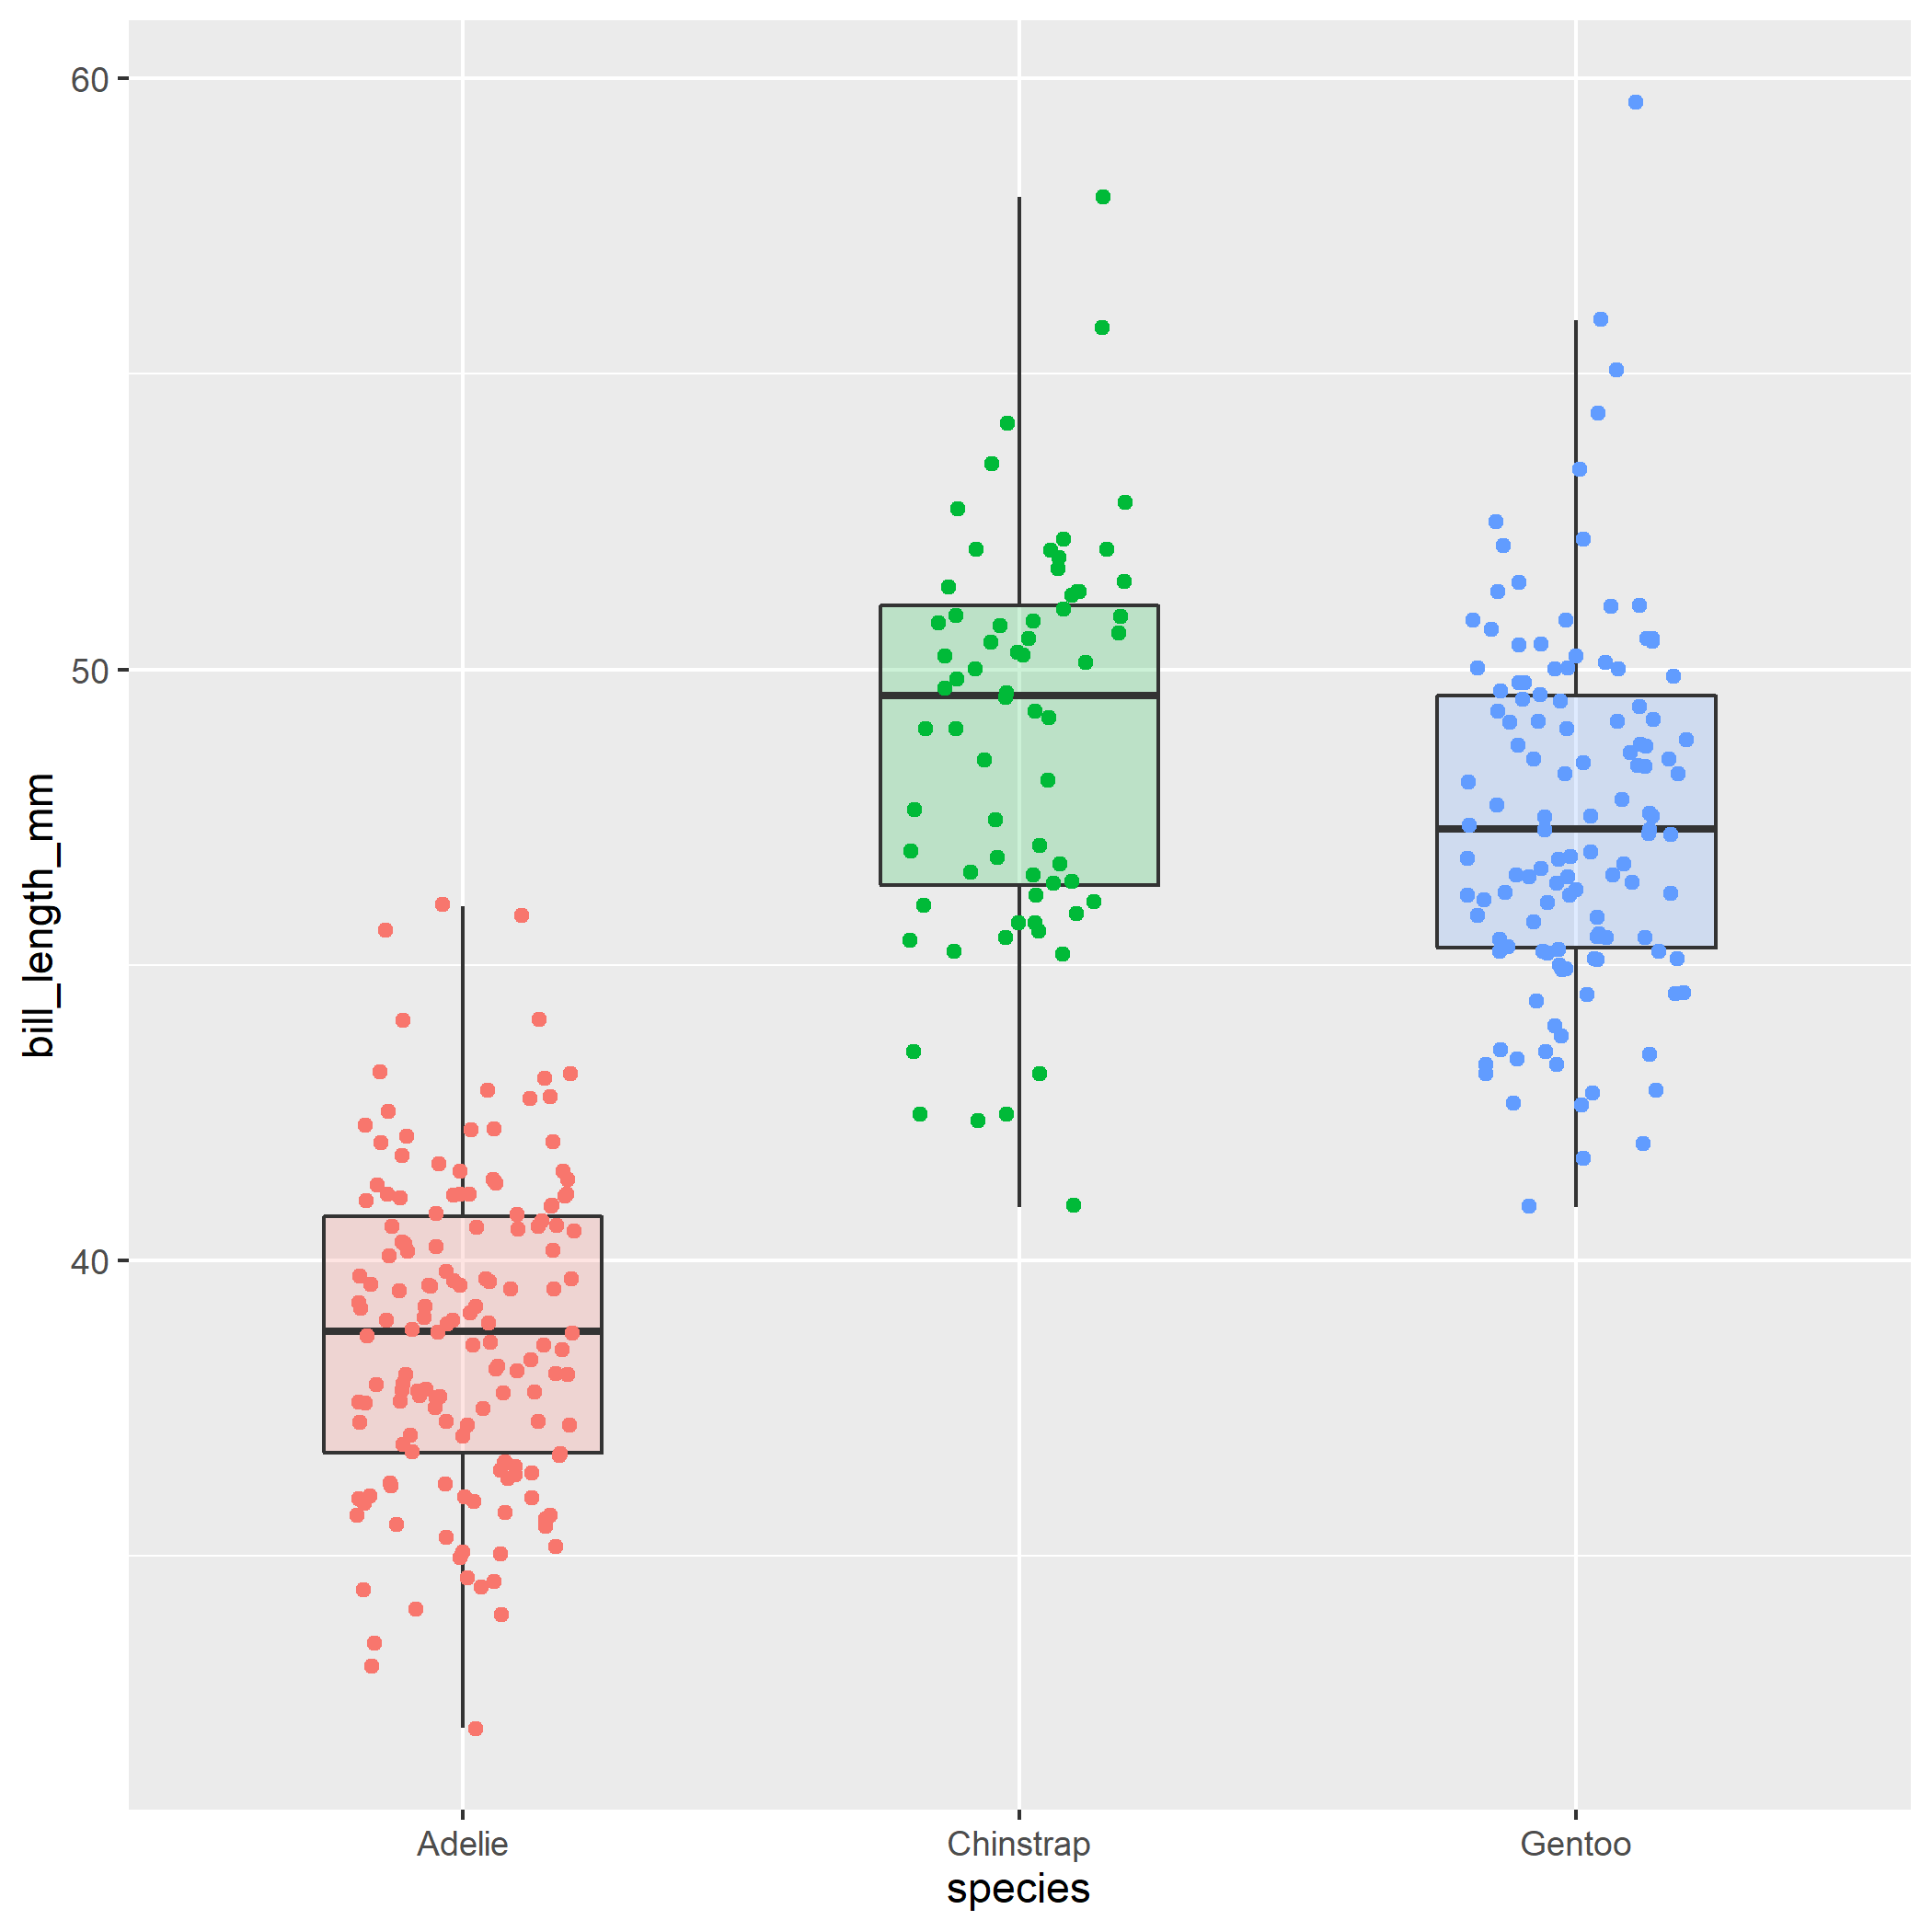
\includegraphics[width=0.8\linewidth]{images/boxandjitter}

\hypertarget{density-and-histogram}{%
\section{Density and histogram}\label{density-and-histogram}}

Compare the following two sets of code

\begin{Shaded}
\begin{Highlighting}[]
\NormalTok{penguins }\SpecialCharTok{\%\textgreater{}\%} 
    \FunctionTok{ggplot}\NormalTok{(}\FunctionTok{aes}\NormalTok{(}\AttributeTok{x=}\NormalTok{bill\_length\_mm, }\AttributeTok{fill=}\NormalTok{species))}\SpecialCharTok{+}
    \FunctionTok{geom\_histogram}\NormalTok{(}\AttributeTok{bins=}\DecValTok{50}\NormalTok{)}
\end{Highlighting}
\end{Shaded}

\begin{Shaded}
\begin{Highlighting}[]
\NormalTok{penguins }\SpecialCharTok{\%\textgreater{}\%} 
    \FunctionTok{ggplot}\NormalTok{(}\FunctionTok{aes}\NormalTok{(}\AttributeTok{x=}\NormalTok{bill\_length\_mm, }\AttributeTok{fill=}\NormalTok{species))}\SpecialCharTok{+}
    \FunctionTok{geom\_histogram}\NormalTok{(}\AttributeTok{bins=}\DecValTok{50}\NormalTok{, }\FunctionTok{aes}\NormalTok{(}\AttributeTok{y=}\NormalTok{..density..))}
\end{Highlighting}
\end{Shaded}

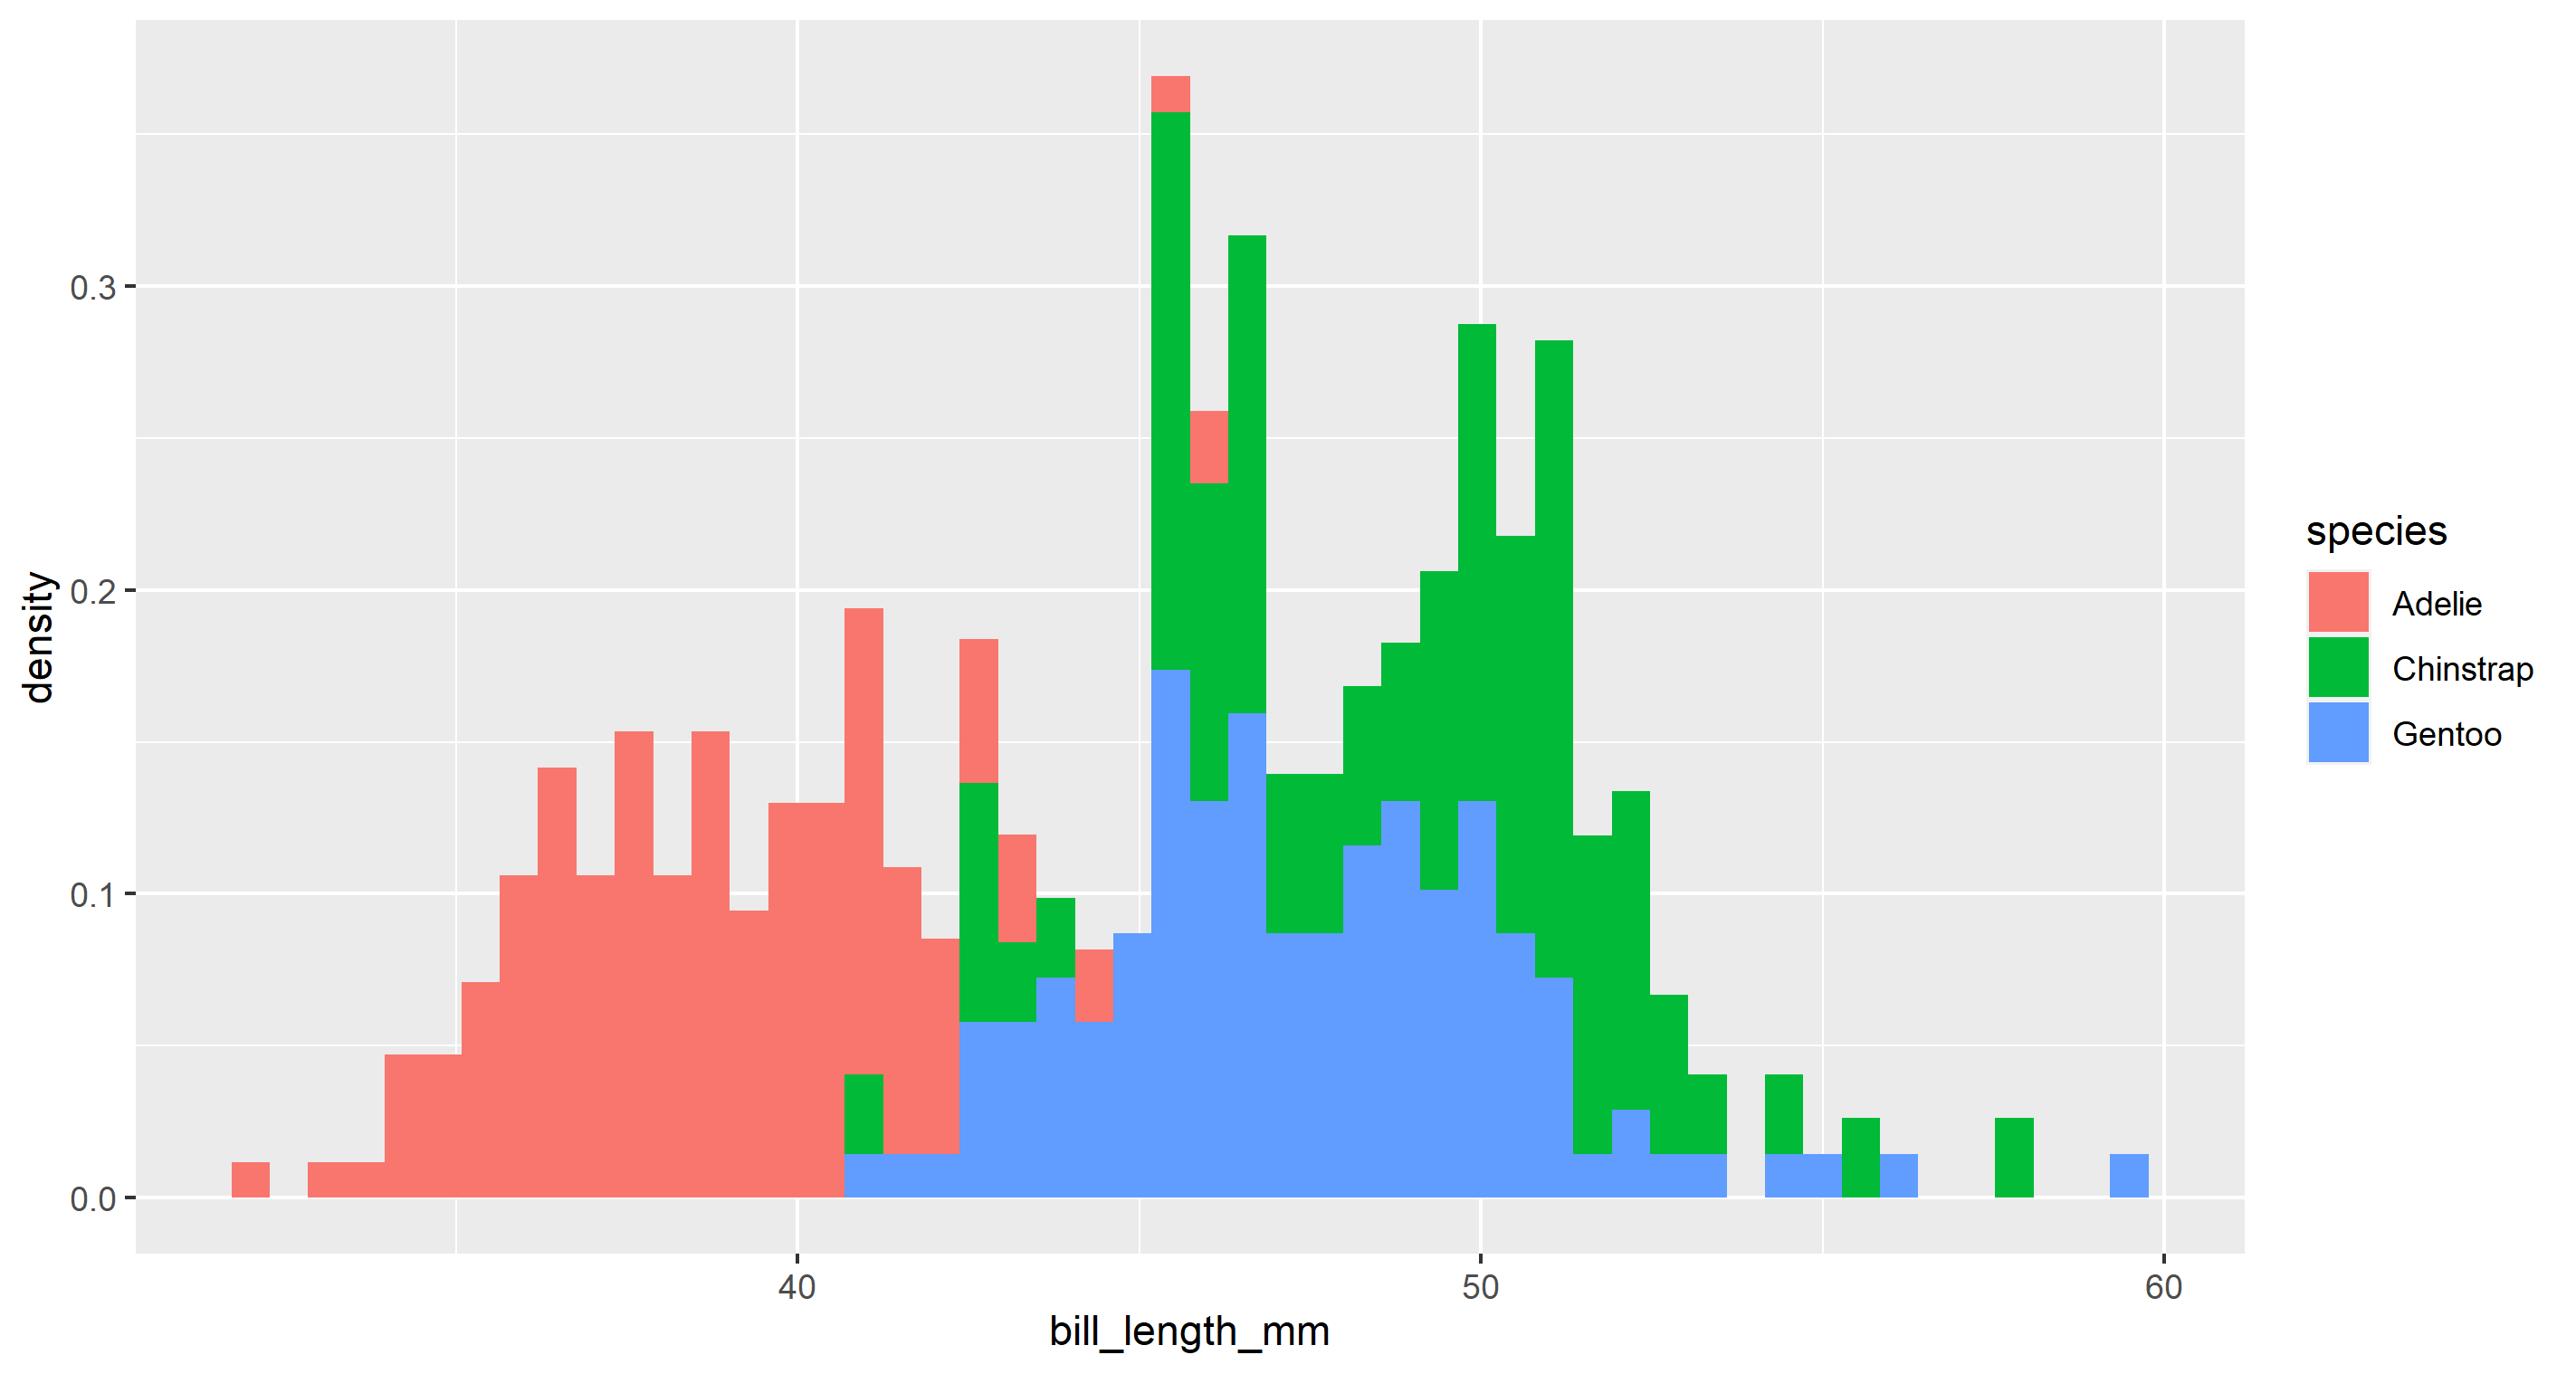
\includegraphics[width=0.8\linewidth]{images/density}

At first you might struggle to see/understand the difference between these two charts. The shapes should be roughly the same.

The first block of code produced a frequency histogram, each bar represents the actual number of observations made within each ``bin'', the second block of code shows the ``relative density'' within each bin. In a density histogram the area under the curve for each sub-group will sum to 1. This allows us to compare distributions and shapes between sub-groups of different sizes. For example there are far fewer Adelie penguins in our dataset, but in a density histogram they occupy the same area of the graph as the other two species.

\hypertarget{more-colours}{%
\section{More Colours}\label{more-colours}}

There are two main differences when it comes to colors in \texttt{ggplot2}. Both arguments, color and fill, can be specified as single color or
assigned to variables.

As you have already seen in this tutorial, variables that are inside the aesthetics are encoded by variables and those that are outside are properties that are unrelated to the variables.

\begin{Shaded}
\begin{Highlighting}[]
\NormalTok{penguins }\SpecialCharTok{\%\textgreater{}\%} 
    \FunctionTok{ggplot}\NormalTok{(}\FunctionTok{aes}\NormalTok{(}\AttributeTok{x=}\NormalTok{bill\_length\_mm))}\SpecialCharTok{+}
    \FunctionTok{geom\_histogram}\NormalTok{(}\AttributeTok{bins=}\DecValTok{50}\NormalTok{, }
                   \FunctionTok{aes}\NormalTok{(}\AttributeTok{y=}\NormalTok{..density..,}
                       \AttributeTok{fill=}\NormalTok{species), }
                   \AttributeTok{colour=}\StringTok{"black"}\NormalTok{)}
\end{Highlighting}
\end{Shaded}

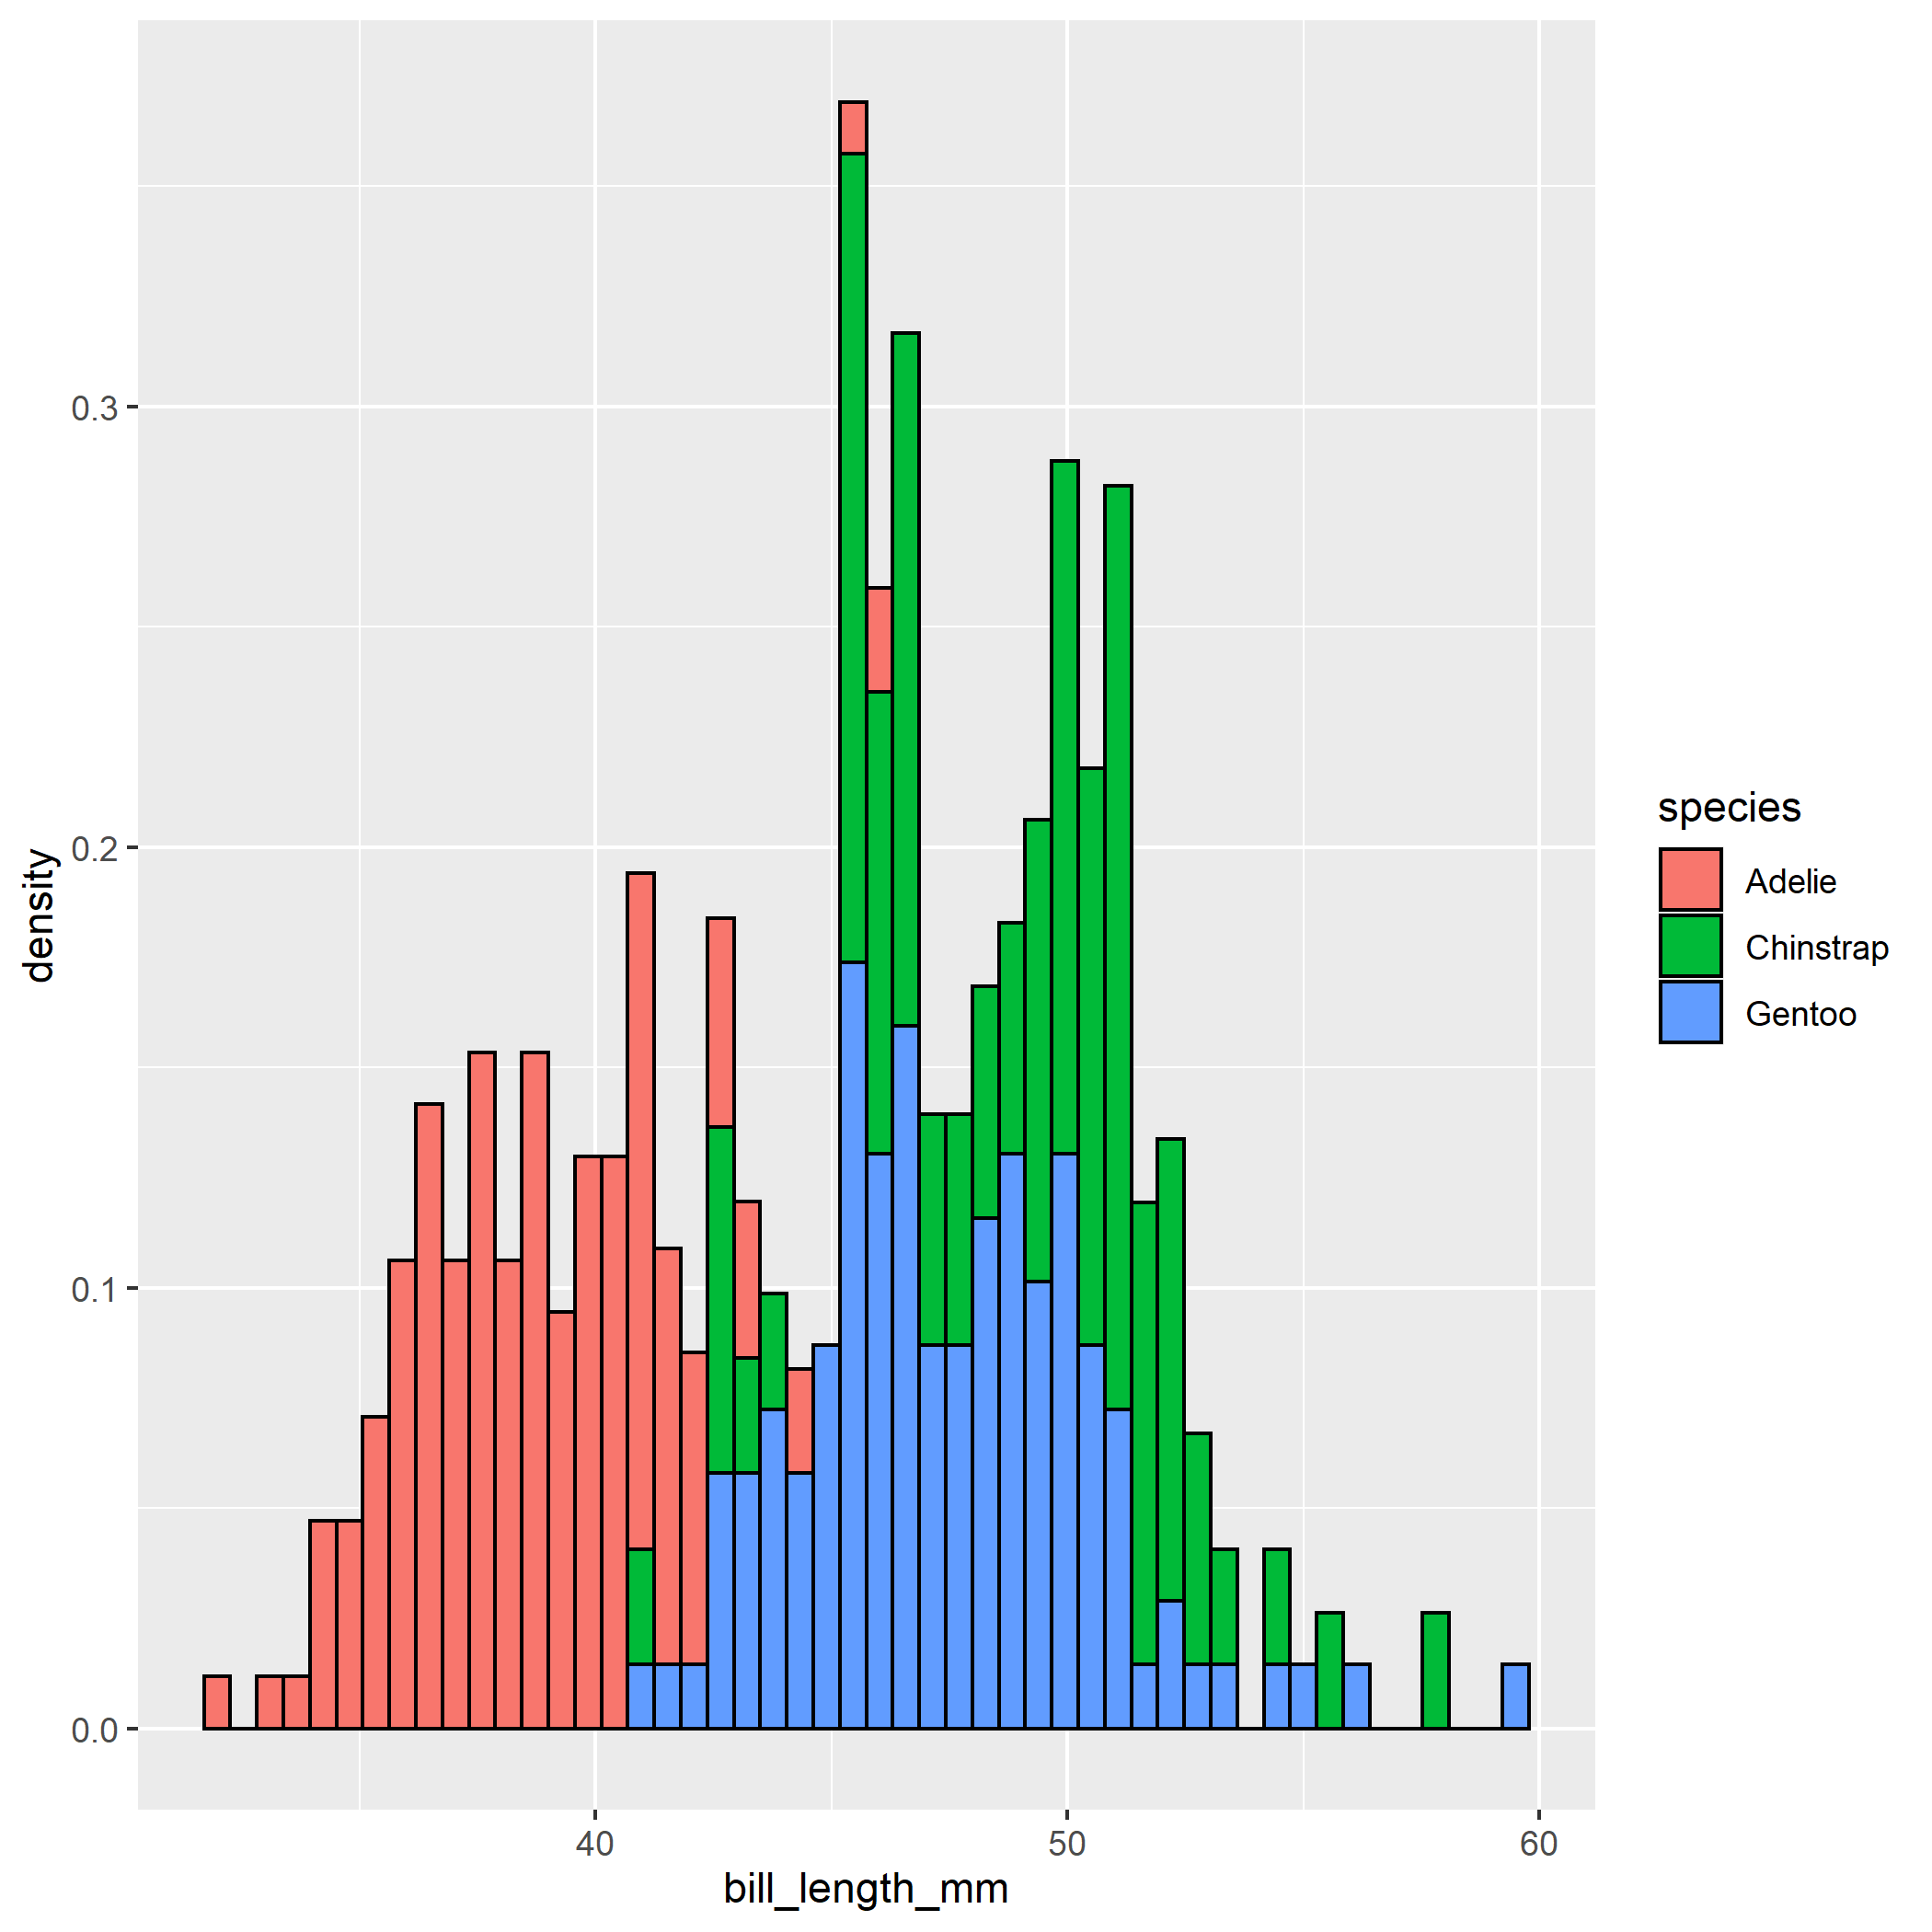
\includegraphics[width=0.8\linewidth]{images/color_fill}

\hypertarget{assign-colours-to-variables}{%
\subsection{Assign colours to variables}\label{assign-colours-to-variables}}

You can specify what colours you want to assign to variables in a number of different ways.

In ggplot2, colors that are assigned to variables are modified via the scale\_color\_* and the scale\_fill\_* functions. In order to use color with your data, most importantly you need to know if you are dealing with a categorical or continuous variable. The color palette should be chosen depending on type of the variable, with sequential or diverging color palettes being used for continuous variables and qualitative color palettes for categorical variables:

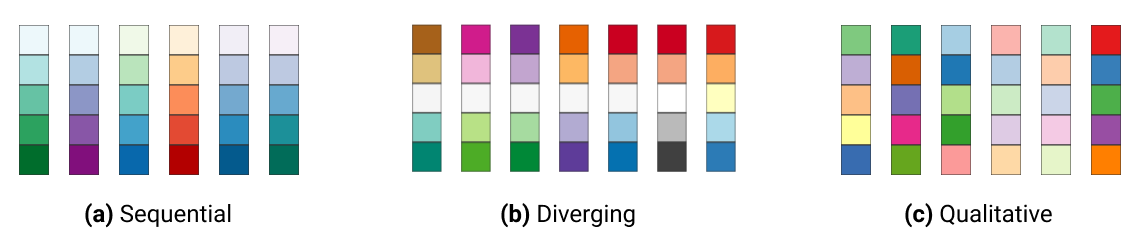
\includegraphics[width=0.8\linewidth]{images/palette}

You can pick your own sets of colours and assign them to a categorical variable. The number of specified colours \textbf{has} to match the number of categories. You can use a wide number of preset colour \href{https://www.datanovia.com/en/blog/awesome-list-of-657-r-color-names/}{names} or you can use \href{https://www.datanovia.com/en/blog/awesome-list-of-hexadecimal-colors-you-should-have/}{hexadecimals}.

\begin{Shaded}
\begin{Highlighting}[]
\NormalTok{penguin\_colours }\OtherTok{\textless{}{-}} \FunctionTok{c}\NormalTok{(}\StringTok{"darkolivegreen4"}\NormalTok{, }\StringTok{"darkorchid3"}\NormalTok{, }\StringTok{"goldenrod1"}\NormalTok{)}

\NormalTok{penguins }\SpecialCharTok{\%\textgreater{}\%} 
  \FunctionTok{ggplot}\NormalTok{(}\FunctionTok{aes}\NormalTok{(}\AttributeTok{x=}\NormalTok{flipper\_length\_mm, }
             \AttributeTok{y =}\NormalTok{ body\_mass\_g))}\SpecialCharTok{+}
  \FunctionTok{geom\_point}\NormalTok{(}\FunctionTok{aes}\NormalTok{(}\AttributeTok{colour=}\NormalTok{species))}\SpecialCharTok{+}
  \FunctionTok{scale\_color\_manual}\NormalTok{(}\AttributeTok{values=}\NormalTok{penguin\_colours)}\SpecialCharTok{+}
  \FunctionTok{theme\_minimal}\NormalTok{()}
\end{Highlighting}
\end{Shaded}

You can also use a range of inbuilt colour palettes:

\begin{Shaded}
\begin{Highlighting}[]
\NormalTok{penguins }\SpecialCharTok{\%\textgreater{}\%} 
  \FunctionTok{ggplot}\NormalTok{(}\FunctionTok{aes}\NormalTok{(}\AttributeTok{x=}\NormalTok{flipper\_length\_mm, }
             \AttributeTok{y =}\NormalTok{ body\_mass\_g))}\SpecialCharTok{+}
  \FunctionTok{geom\_point}\NormalTok{(}\FunctionTok{aes}\NormalTok{(}\AttributeTok{colour=}\NormalTok{species))}\SpecialCharTok{+}
  \FunctionTok{scale\_color\_brewer}\NormalTok{(}\AttributeTok{palette=}\StringTok{"Set1"}\NormalTok{)}\SpecialCharTok{+}
  \FunctionTok{theme\_minimal}\NormalTok{()}
\end{Highlighting}
\end{Shaded}

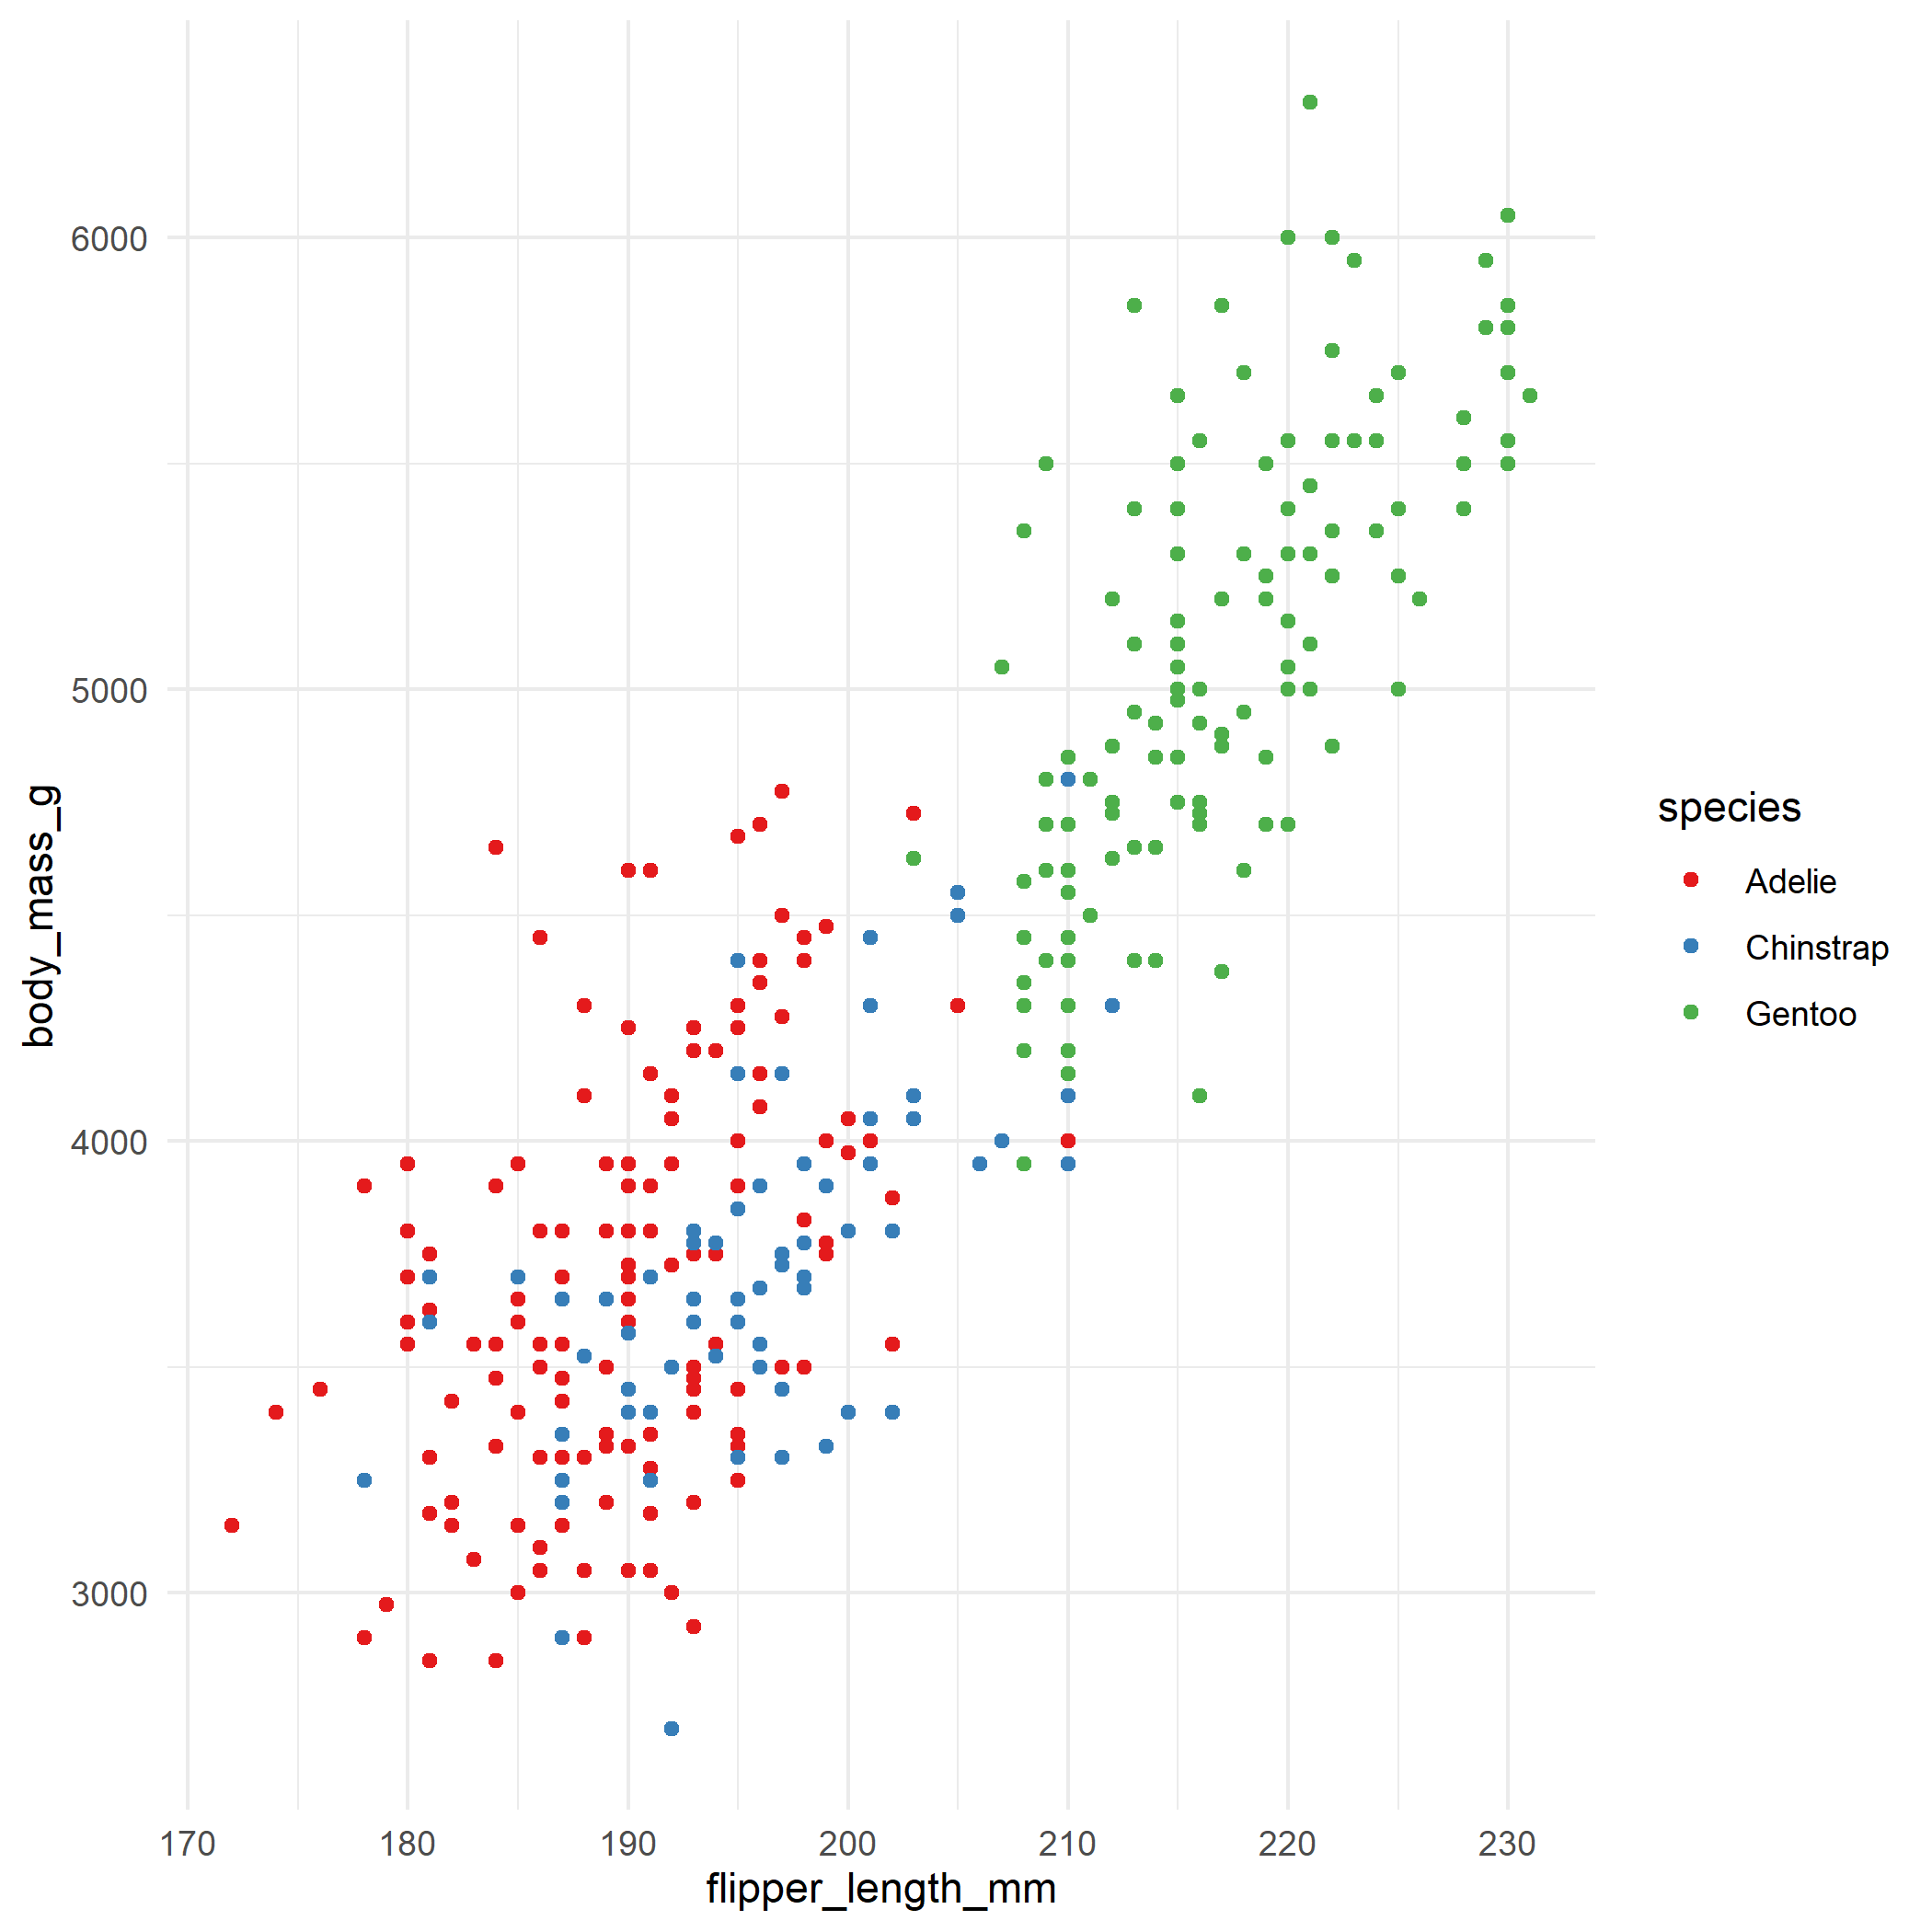
\includegraphics[width=0.8\linewidth]{images/penguinspalette}

\begin{rmdwarning}
You can explore all schemes available with the command
\texttt{RColorBrewer::display.brewer.all()}
\end{rmdwarning}

There are also many, many extensions that provide additional colour palettes. Some of my favourite packages include \texttt{ggsci}(\citet{R-ggsci}) and \texttt{wesanderson}(\citet{R-wesanderson}).

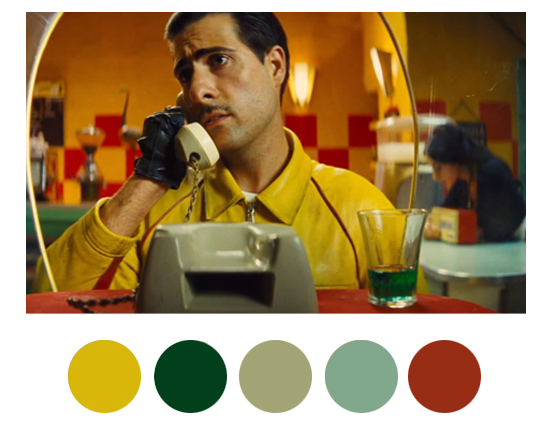
\includegraphics[width=0.8\linewidth]{images/wesanderson}

\hypertarget{accessibility}{%
\subsection{Accessibility}\label{accessibility}}

It's very easy to get carried away with colour palettes, but you should remember at all times that your figures must be accessible. One way to check how accessible your figures are is to use a colour blindness checker \citet{R-colorBlindness}

\begin{Shaded}
\begin{Highlighting}[]
\FunctionTok{library}\NormalTok{(colorBlindness)}
\FunctionTok{cvdPlot}\NormalTok{() }\CommentTok{\# will automatically run on the last plot you made}
\end{Highlighting}
\end{Shaded}

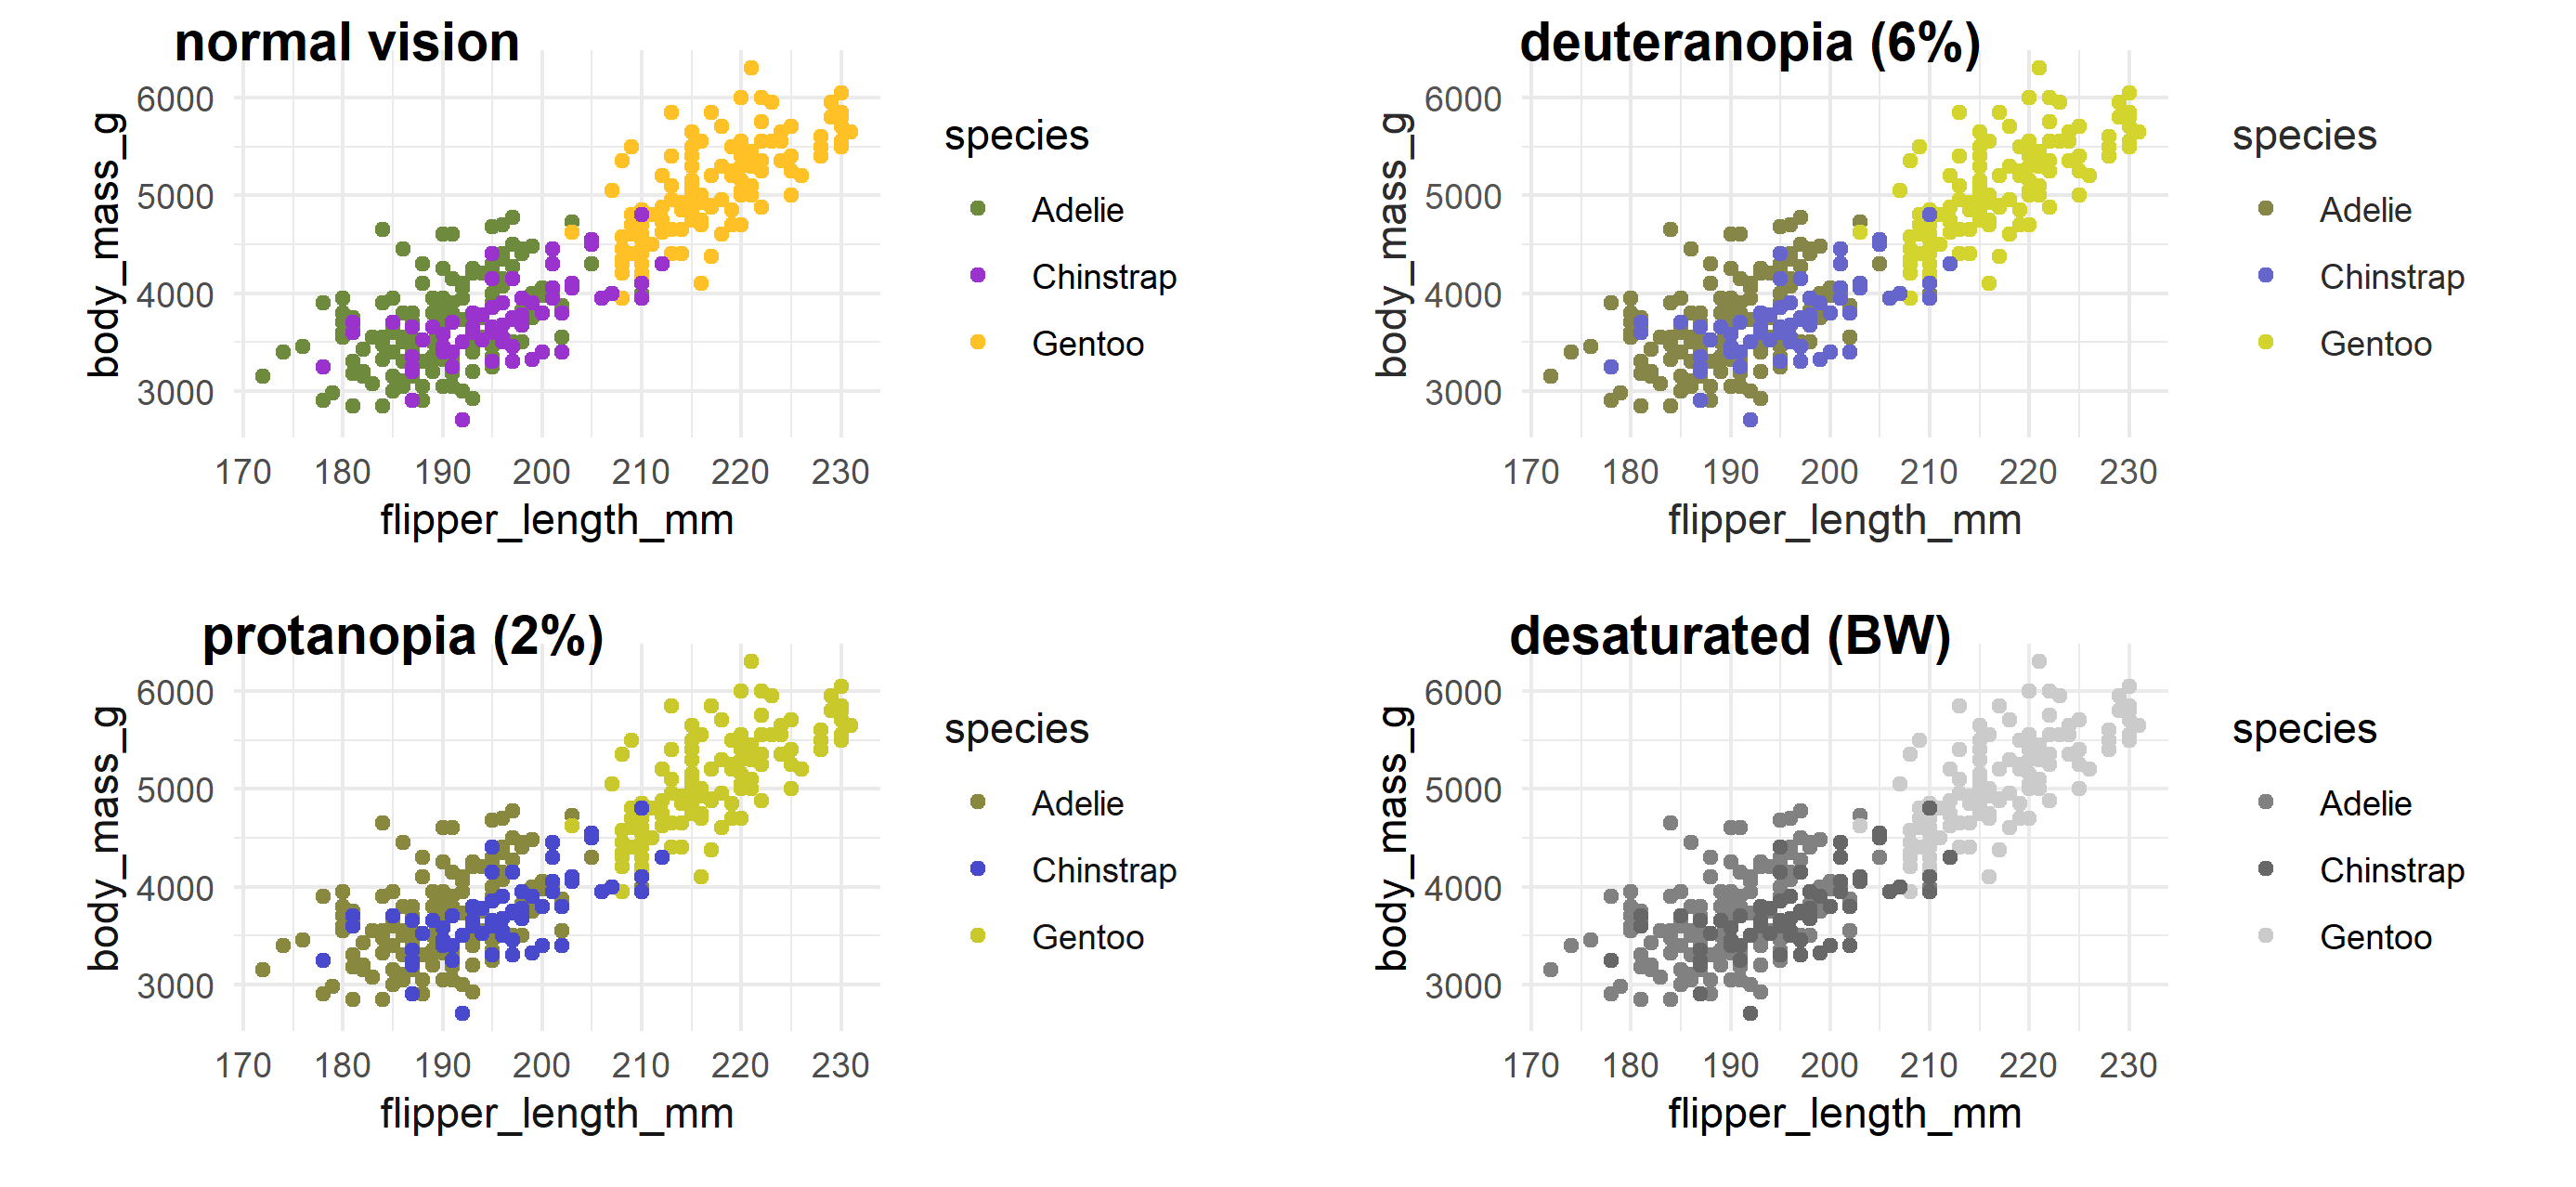
\includegraphics[width=0.8\linewidth]{images/colorblind}

\hypertarget{guides-to-visual-accessibility}{%
\subsection{Guides to visual accessibility}\label{guides-to-visual-accessibility}}

Using colours to tell categories apart can be useful, but as we can see in the example above, you should choose carefully. Other aesthetics which you can access in your geoms include \texttt{shape}, and \texttt{size} - you can combine these in complimentary ways to enhance the accessibility of your plots. Here is a hierarchy of ``interpretability'' for different types of data

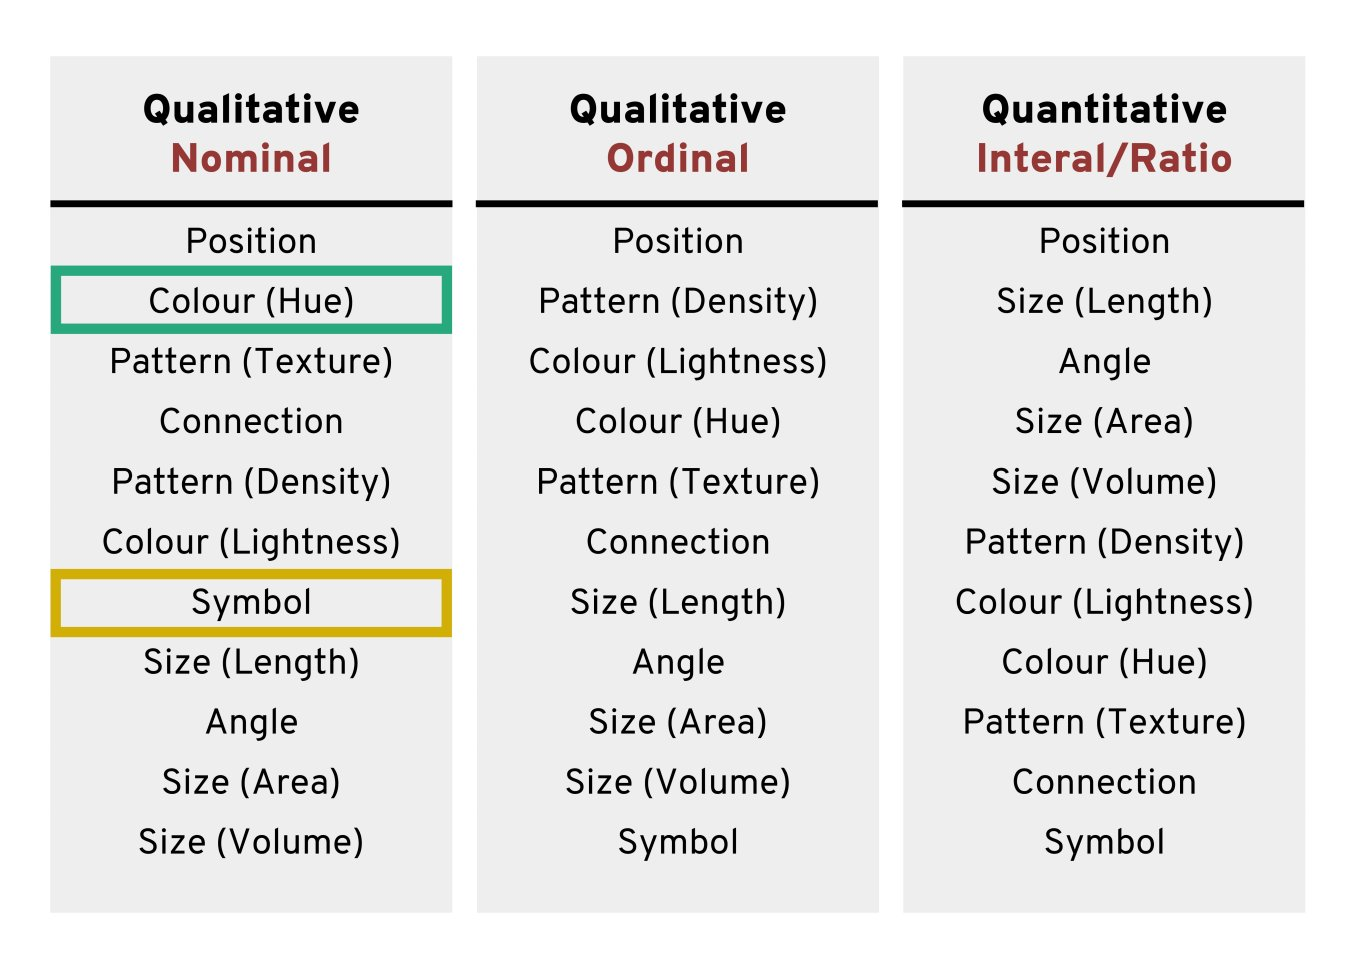
\includegraphics[width=0.8\linewidth]{images/list}

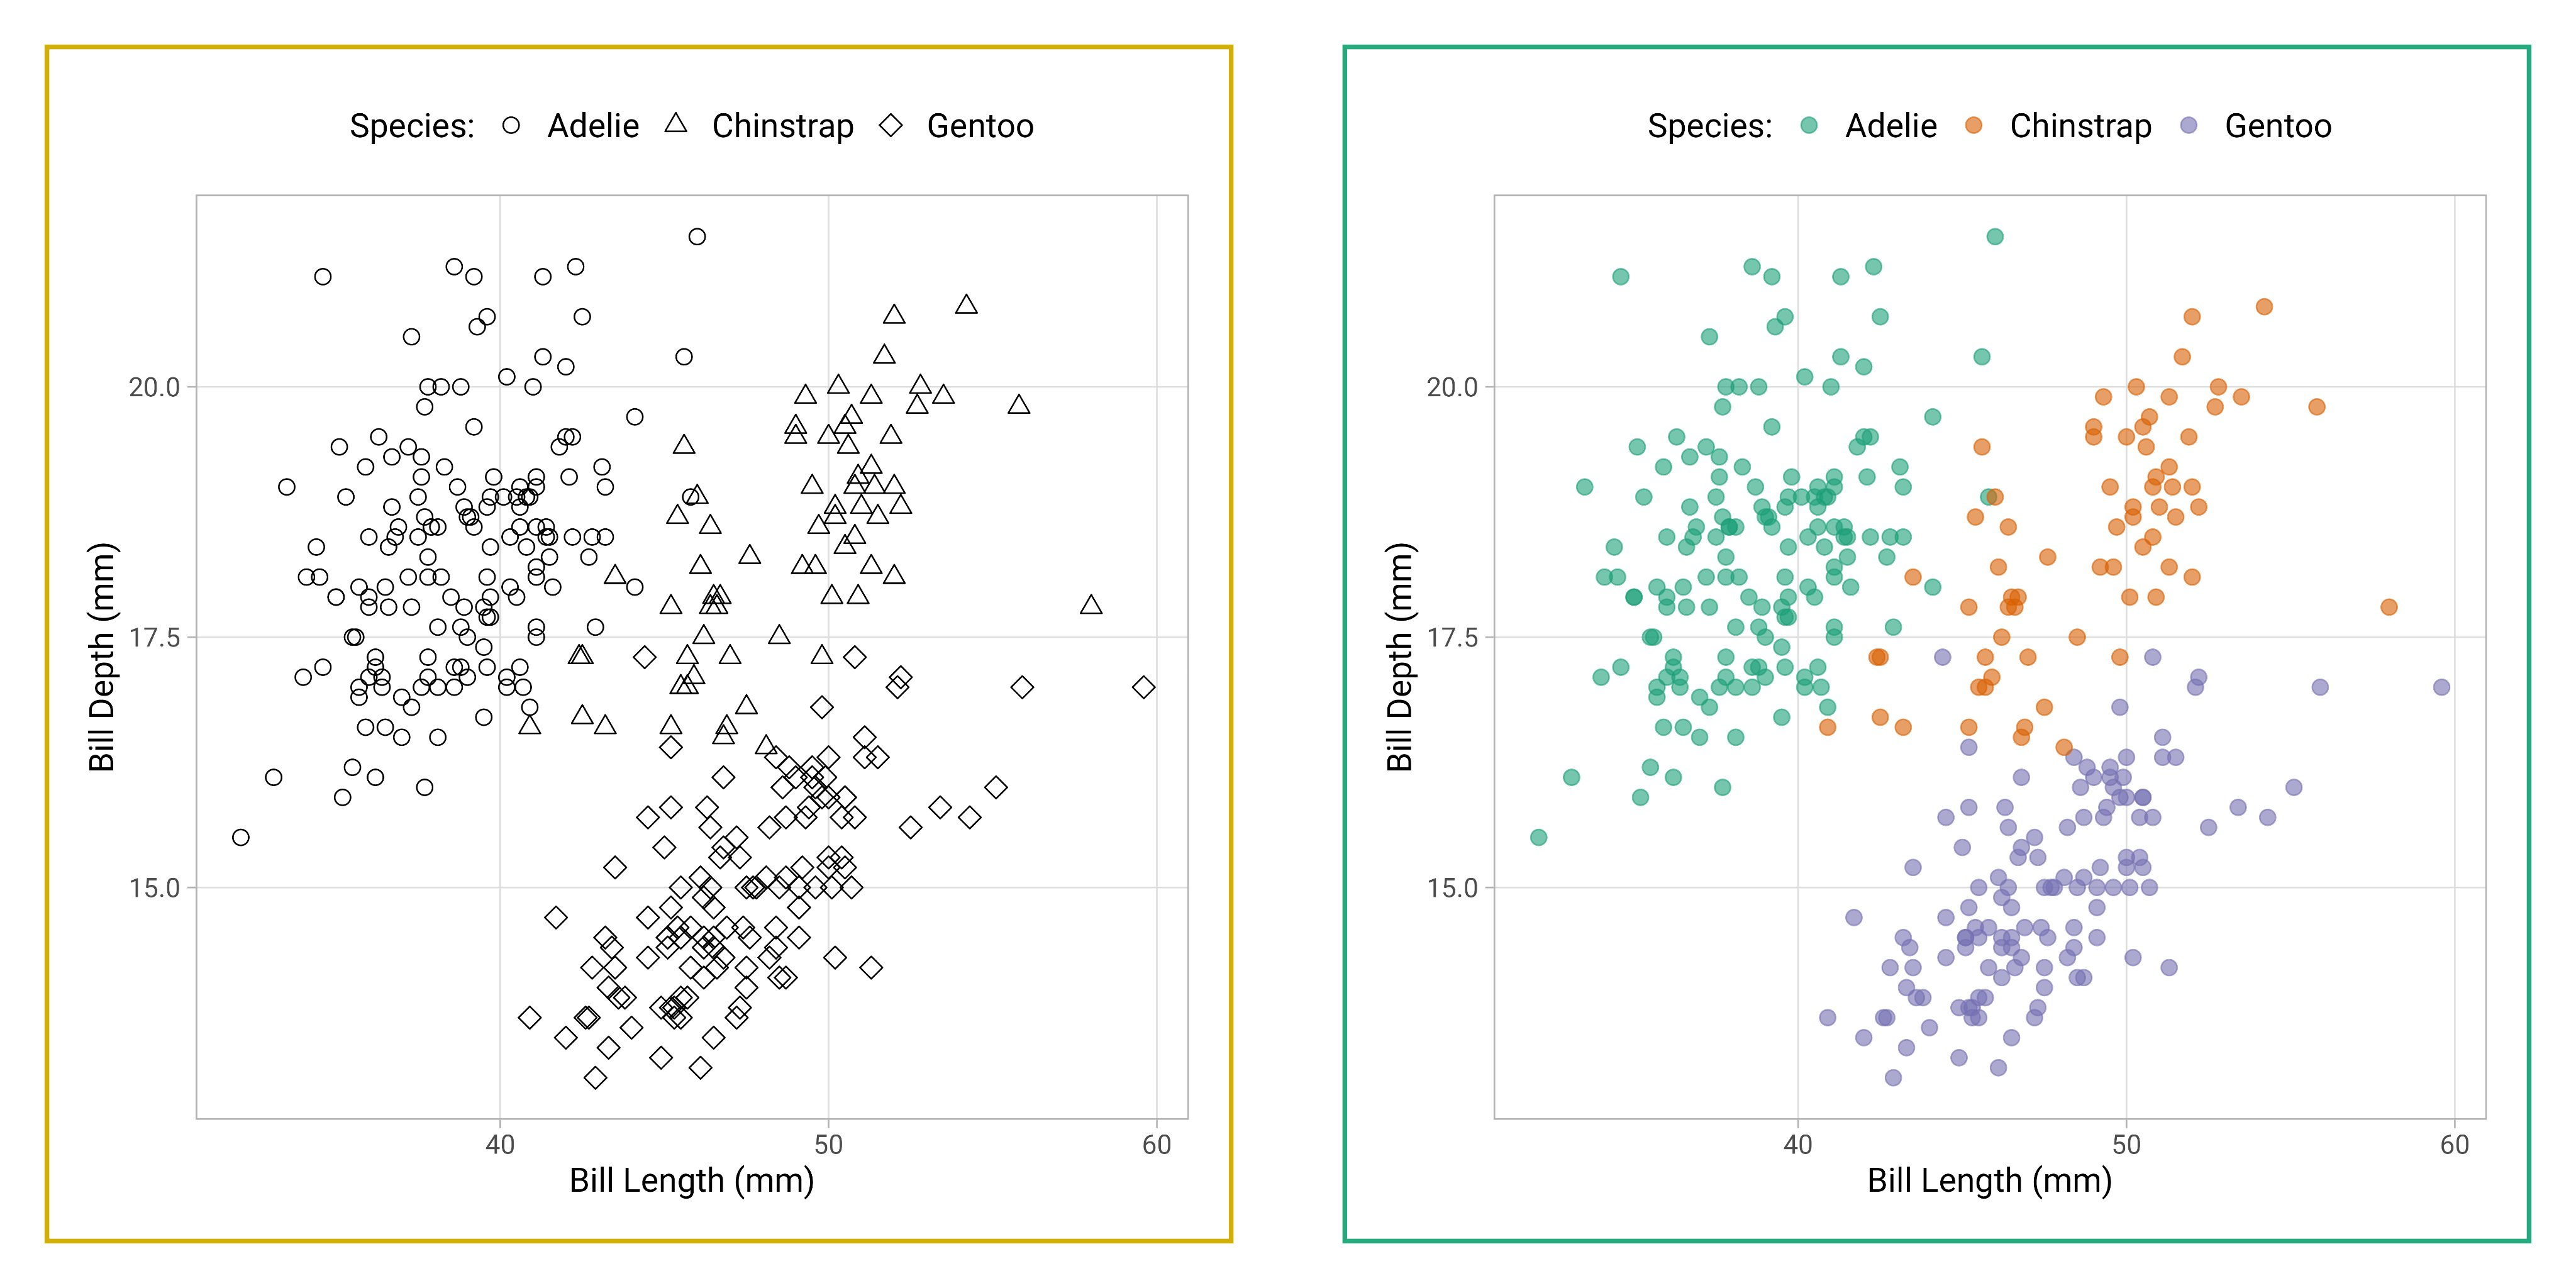
\includegraphics[width=0.8\linewidth]{images/shape_v_colour}

\hypertarget{patchwork}{%
\section{Patchwork}\label{patchwork}}

There are many times you might want to combine figures into multi-panel plots. Probably the easiest way to do this is with the \texttt{patchwork} package (\citet{R-patchwork}).

\begin{Shaded}
\begin{Highlighting}[]
\NormalTok{p1 }\OtherTok{\textless{}{-}}\NormalTok{ penguins }\SpecialCharTok{\%\textgreater{}\%} 
  \FunctionTok{ggplot}\NormalTok{(}\FunctionTok{aes}\NormalTok{(}\AttributeTok{x=}\NormalTok{flipper\_length\_mm, }
             \AttributeTok{y =}\NormalTok{ bill\_length\_mm))}\SpecialCharTok{+}
  \FunctionTok{geom\_point}\NormalTok{(}\FunctionTok{aes}\NormalTok{(}\AttributeTok{colour=}\NormalTok{species))}\SpecialCharTok{+}
  \FunctionTok{scale\_color\_manual}\NormalTok{(}\AttributeTok{values=}\NormalTok{penguin\_colours)}\SpecialCharTok{+}
  \FunctionTok{theme\_minimal}\NormalTok{()}

\NormalTok{p2 }\OtherTok{\textless{}{-}}\NormalTok{ penguins }\SpecialCharTok{\%\textgreater{}\%} 
  \FunctionTok{ggplot}\NormalTok{(}\FunctionTok{aes}\NormalTok{(}\AttributeTok{x=}\NormalTok{bill\_depth\_mm, }
             \AttributeTok{y =}\NormalTok{ bill\_length\_mm))}\SpecialCharTok{+}
  \FunctionTok{geom\_point}\NormalTok{(}\FunctionTok{aes}\NormalTok{(}\AttributeTok{colour=}\NormalTok{species))}\SpecialCharTok{+}
  \FunctionTok{scale\_color\_manual}\NormalTok{(}\AttributeTok{values=}\NormalTok{penguin\_colours)}\SpecialCharTok{+}
  \FunctionTok{theme\_minimal}\NormalTok{()}

\NormalTok{p3 }\OtherTok{\textless{}{-}}\NormalTok{ penguins }\SpecialCharTok{\%\textgreater{}\%}     
  \FunctionTok{group\_by}\NormalTok{(sex,species) }\SpecialCharTok{\%\textgreater{}\%} 
    \FunctionTok{summarise}\NormalTok{(}\AttributeTok{n=}\FunctionTok{n}\NormalTok{()) }\SpecialCharTok{\%\textgreater{}\%} 
     \FunctionTok{drop\_na}\NormalTok{(sex) }\SpecialCharTok{\%\textgreater{}\%} 
     \FunctionTok{ggplot}\NormalTok{(}\FunctionTok{aes}\NormalTok{(}\AttributeTok{x=}\NormalTok{species, }\AttributeTok{y=}\NormalTok{n)) }\SpecialCharTok{+} 
  \FunctionTok{geom\_col}\NormalTok{(}\FunctionTok{aes}\NormalTok{(}\AttributeTok{fill=}\NormalTok{sex), }
               \AttributeTok{width=}\FloatTok{0.8}\NormalTok{,}
               \AttributeTok{position=}\FunctionTok{position\_dodge}\NormalTok{(}\AttributeTok{width=}\FloatTok{0.9}\NormalTok{), }
               \AttributeTok{alpha=}\FloatTok{0.6}\NormalTok{)}\SpecialCharTok{+}
     \FunctionTok{scale\_fill\_manual}\NormalTok{(}\AttributeTok{values=}\FunctionTok{c}\NormalTok{(}\StringTok{"darkorange1"}\NormalTok{, }\StringTok{"azure4"}\NormalTok{))}\SpecialCharTok{+}
     \FunctionTok{theme\_classic}\NormalTok{()}

\FunctionTok{library}\NormalTok{(patchwork)}

\NormalTok{ (p1}\SpecialCharTok{+}\NormalTok{p2)}\SpecialCharTok{/}\NormalTok{p3}\SpecialCharTok{+}
  \FunctionTok{plot\_layout}\NormalTok{(}\AttributeTok{guides =} \StringTok{"collect"}\NormalTok{) }
\end{Highlighting}
\end{Shaded}

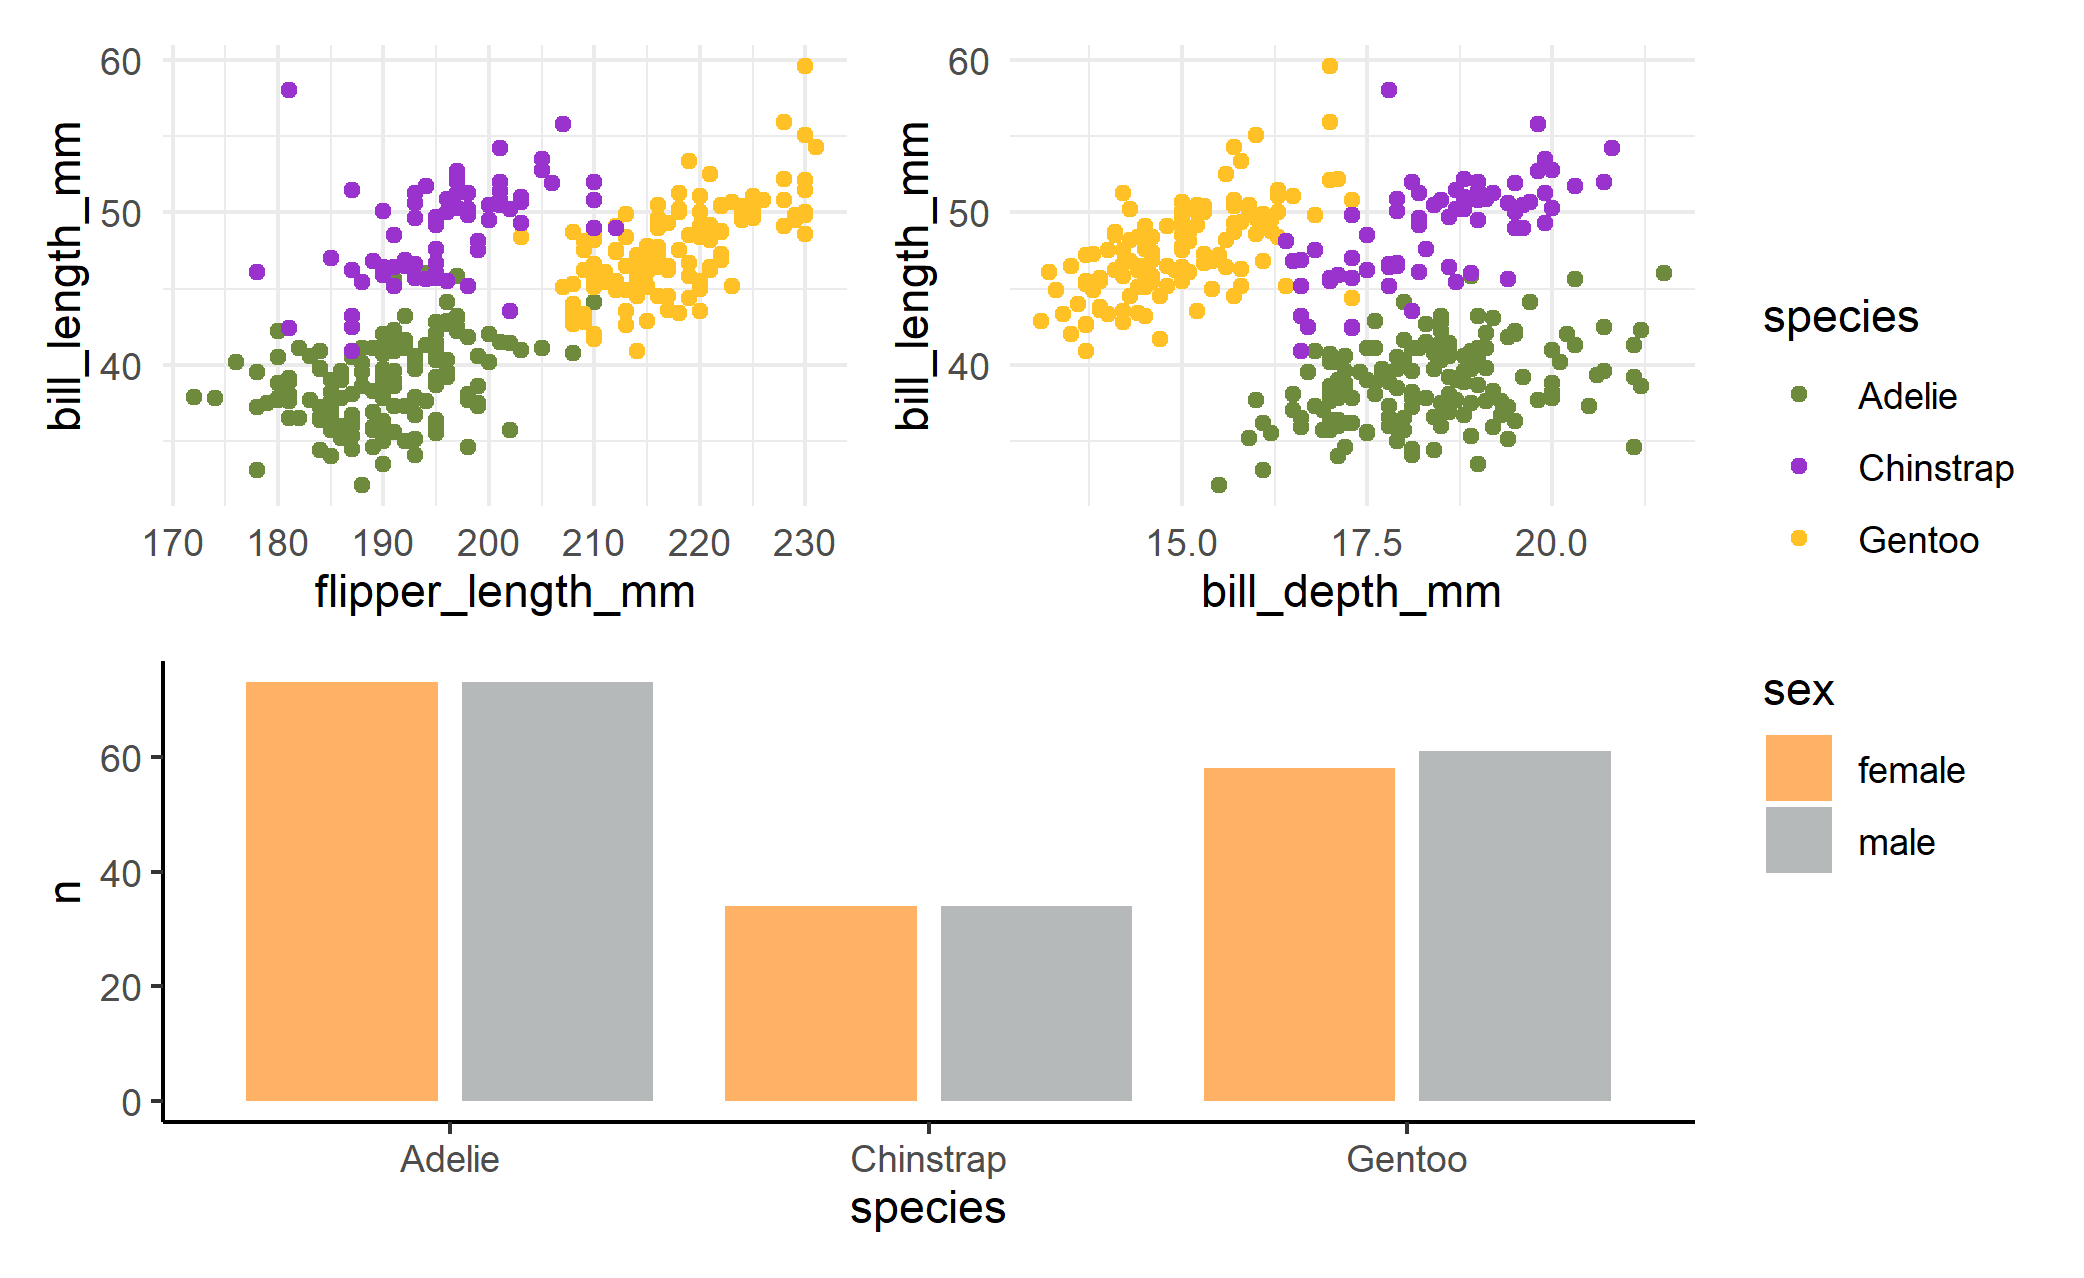
\includegraphics[width=0.9\linewidth]{images/patchwork}

\hypertarget{test}{%
\section{Test}\label{test}}

\begin{rmdquestion}
Challenge - How close can you get to replicating the figure below?

Make sure to use the tips and links at the end of this chapter
\end{rmdquestion}

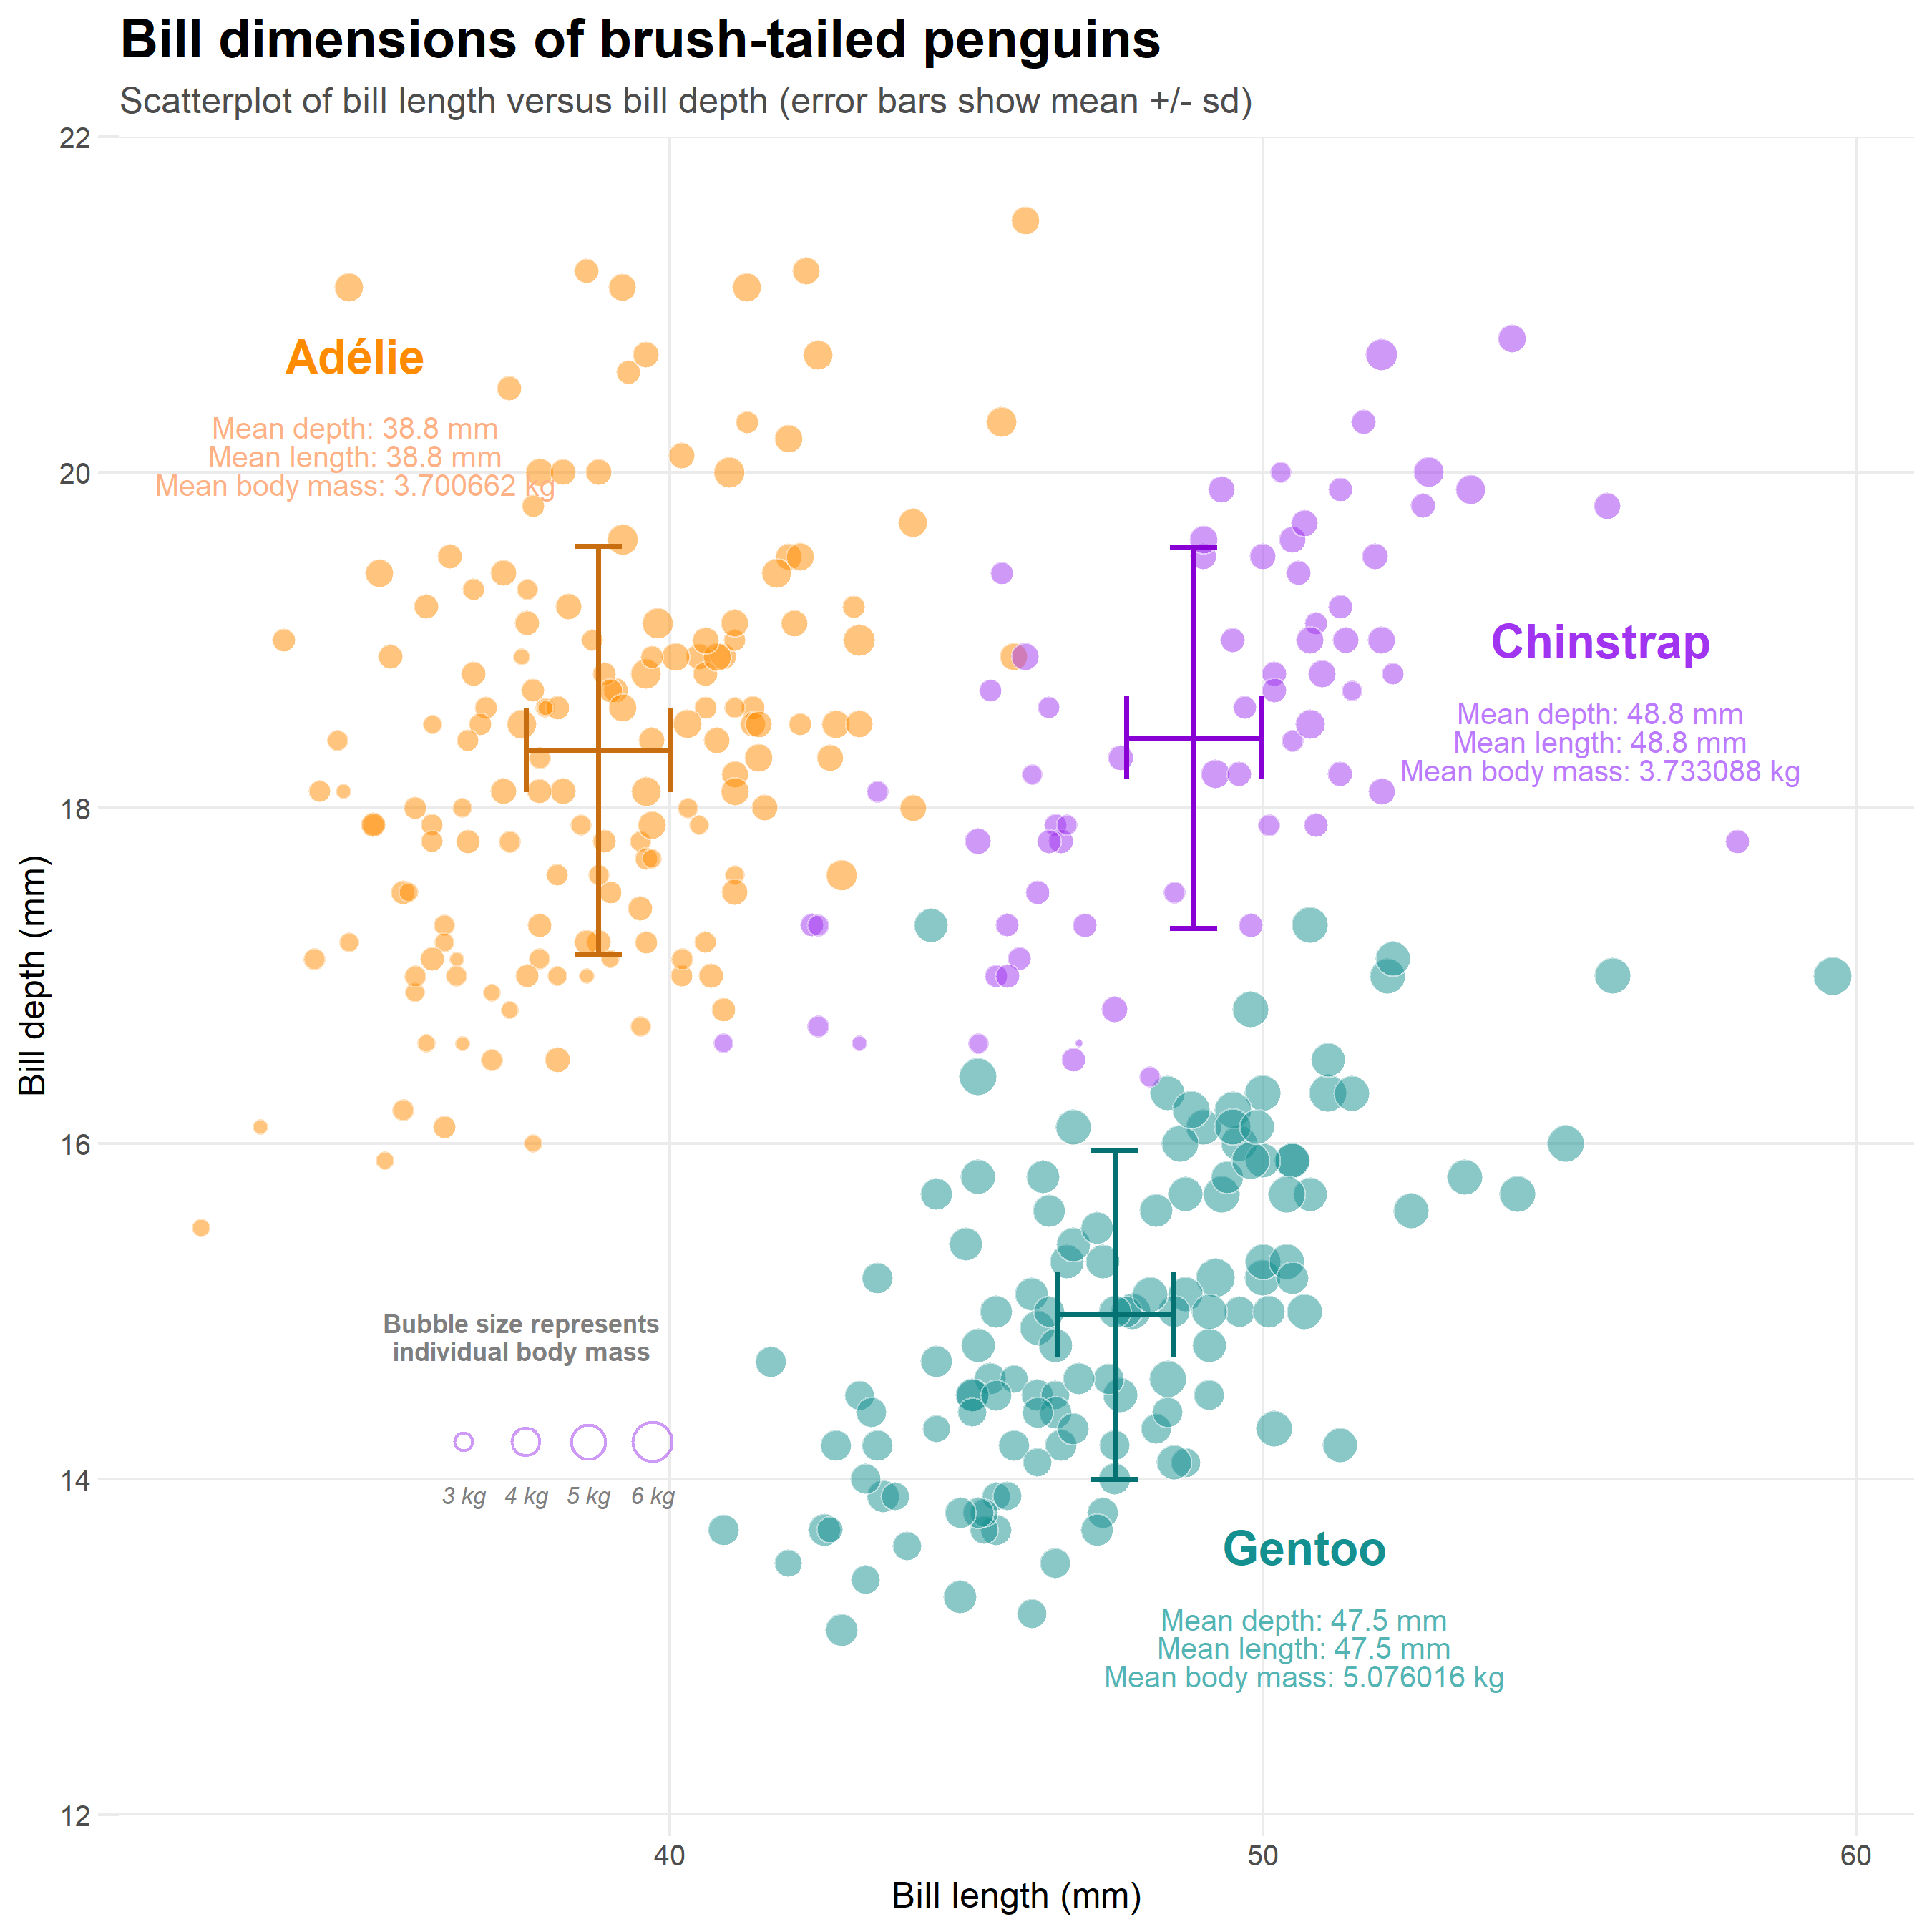
\includegraphics[width=1\linewidth]{images/ambitious}

\hypertarget{saving}{%
\section{Saving}\label{saving}}

One of the easiest ways to save a figure you have made is with the \texttt{ggsave()} function. By default it will save the last plot you made on the screen.

You should specify the output path to your \textbf{figures} folder, then provide a file name. Here I have decided to call my plot \emph{plot} (imaginative!) and I want to save it as a .PNG image file. I can also specify the resolution (dpi 300 is good enough for most computer screens).

\begin{Shaded}
\begin{Highlighting}[]
\FunctionTok{ggsave}\NormalTok{(}\StringTok{"figures/plot.png"}\NormalTok{, }\AttributeTok{dpi=}\DecValTok{300}\NormalTok{)}
\end{Highlighting}
\end{Shaded}

\hypertarget{quitting-3}{%
\section{Quitting}\label{quitting-3}}

\begin{rmdwarning}
Make sure you have saved your script!
\end{rmdwarning}

\begin{rmdquestion}
Download your saved figure from RStudio Cloud and submit it to
Blackboard ``Week Four Test''
\end{rmdquestion}

\hypertarget{summing-up-ggplot}{%
\section{Summing up ggplot}\label{summing-up-ggplot}}

\hypertarget{what-we-learned-1}{%
\subsection{What we learned}\label{what-we-learned-1}}

You have learned

\begin{itemize}
\item
  The anatomy of ggplots
\item
  How to add geoms on different layers
\item
  How to use colour, colour palettes, facets, labels and themes
\item
  Putting together multiple figures
\item
  How to save and export images
\end{itemize}

You have primarily worked with \texttt{tidyverse} and the package

\begin{itemize}
\tightlist
\item
  \texttt{ggplot2} \citet{R-ggplot2}
\end{itemize}

As well as:

\begin{itemize}
\item
  \texttt{colorBlindness} \citet{R-colorBlindness}
\item
  \texttt{patchwork} \citet{R-patchwork}
\end{itemize}

\hypertarget{further-reading-guides-and-tips}{%
\subsection{Further Reading, Guides and tips}\label{further-reading-guides-and-tips}}

\href{https://www.rstudio.com/resources/cheatsheets/}{R Cheat Sheets}

\citet{dataviz} \url{https://clauswilke.com/dataviz/}

\emph{this book tells you everything you need to know about presenting your figures for accessbility and clarity}

\url{https://www.cedricscherer.com/2019/08/05/a-ggplot2-tutorial-for-beautiful-plotting-in-r/}

\emph{an incredibly handy ggplot guide for how to build and improve your figures}

\citet{ggplot} \url{https://ggplot2-book.org/}

\emph{the original Hadley Wickham book on ggplot2}

\hypertarget{reports-with-rmarkdown-week-five}{%
\chapter{Reports with Rmarkdown: Week Five}\label{reports-with-rmarkdown-week-five}}

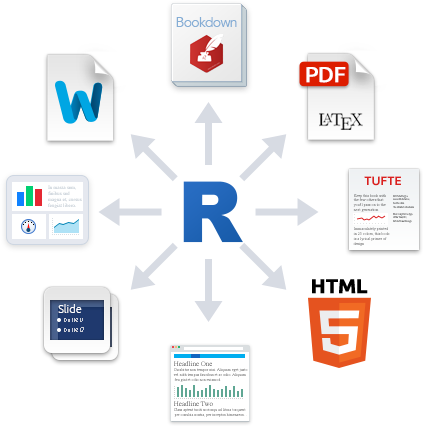
\includegraphics[width=1\linewidth]{images/rmarkdownoutputformats}

R Markdown is a widely-used tool for creating automated, reproducible, and share-worthy outputs, such as reports. It can generate static or interactive outputs, in Word, pdf, html, powerpoint, and other formats.

An R Markdown script combines R code and text such that the script actually becomes your output document. You can create an entire formatted document, including narrative text (can be dynamic to change based on your data), tables, figures, bullets/numbers, bibliographies, etc.

Documents produced with Rmarkdown, allow analyses to be included easily - and make the link between raw data, analysis \& and a published report \emph{completely reproducible}.

With Rmarkdown we can make reproducible html, word, pdf, powerpoints or websites and dashboards\footnote{(\url{https://rmarkdown.rstudio.com/lesson-9.html})}

\textbf{To make your Rmd publish - hit the knit button at the top of the doc}

\hypertarget{format}{%
\subsection{Format}\label{format}}

\begin{itemize}
\item
  Go to RStudio Cloud and open \textbf{Week 5 - Rmarkdown}
\item
  Follow the instructions carefully - and assemble your Rmarkdown file bit by bit - when prompted to `knit' the document do it. We will then observed the results and might make changes.
\end{itemize}

\hypertarget{background-to-rmarkdown}{%
\section{Background to Rmarkdown}\label{background-to-rmarkdown}}

\begin{itemize}
\item
  Markdown is a ``language'' that allows you to write a document using plain text, that can be converted to html and other formats. It is not specific to R. Files written in Markdown have a `.md' extension.
\item
  R Markdown: is a variation on markdown that is specific to R - it allows you to write a document using markdown to produce text and to embed R code and display their outputs. R Markdown files have `.Rmd' extension.
\item
  rmarkdown - the package: This is used by R to render the .Rmd file into the desired output. It's focus is converting the markdown (text) syntax, so we also need\ldots{}
\item
  knitr: This R package will read the code chunks, execute it, and `knit' it back into the document. This is how tables and graphs are included alongside the text.
\item
  Pandoc: Finally, pandoc actually convert the output into word/pdf/powerpoint etc. It is a software separate from R but is installed automatically with RStudio.
\end{itemize}

Most of this process happens in the background (you do not need to know all these steps!) and it involves feeding the .Rmd file to knitr, which executes the R code chunks and creates a new .md (markdown) file which includes the R code and its rendered output. The .md file is then processed by pandoc to create the finished product: a Microsoft Word document, HTML file, powerpoint document, pdf, etc.
When using RStudio Cloud - all of these features are pre-loaded - if you take your R journey further in the future and install a copy of R and RStudio on your own computer you might have to do a little setting up to get this working.


\includegraphics[width=0.8\linewidth]{images/0_rmd}

\hypertarget{starting-a-new-rmd-file}{%
\section{Starting a new Rmd file}\label{starting-a-new-rmd-file}}

In RStudio, if you open a new R markdown file, start with `File', then `New file' then `R markdown\ldots{}'.

R Studio will give you some output options to pick from. In the example below we select ``HTML'' because we want to create an html document. The title and the author names are not important. If the output document type you want is not one of these, don't worry - you can just pick any one and change it in the script later.

\textbf{For now open the markdown file which I have made in the Markdown sub-folder}.

\begin{rmdwarning}
The working directory for .rmd files is a little different to working
with scripts.

With a .Rmd file, the working directory is wherever the Rmd file itself
is saved.

For example if you have your .Rmd file in a subfolder
\textasciitilde/markdownfiles/markdown.Rmd the code for
read\_csv(``data/data.csv'') within the markdown will look for a .csv
file in a subfolder called data \emph{inside} the \texttt{markdownfiles}
folder and not the root project folder where the .RProj file lives.

So we have two options when using .Rmd files

\begin{enumerate}
\def\labelenumi{\arabic{enumi})}
\item
  Don't put the .Rmd file in a subfolder and make sure it lives in the
  same directory as your .RProj file
\item
  Use the `here' package to describe file locations - more later
\end{enumerate}
\end{rmdwarning}

\hypertarget{r-markdown-parts}{%
\section{R Markdown parts}\label{r-markdown-parts}}

An R Markdown document can be edited in RStudio just like a standard R script. When you start a new R Markdown script, RStudio tries to be helpful by showing a template which explains the different section of an R Markdown script.

The below is what appears when starting a new Rmd script intended to produce an html output.

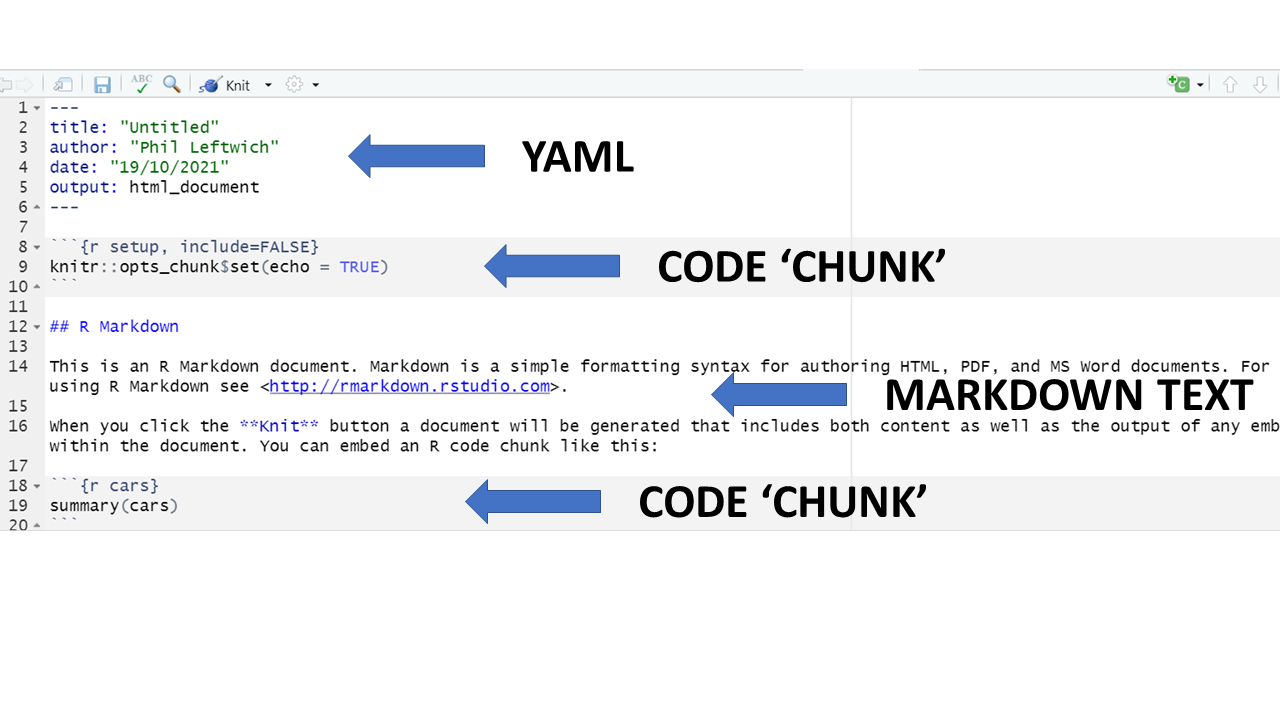
\includegraphics[width=0.8\linewidth]{images/templatermd}

As you can see, there are three basic components to any Rmd file: YAML, Markdown text, and R code chunks.

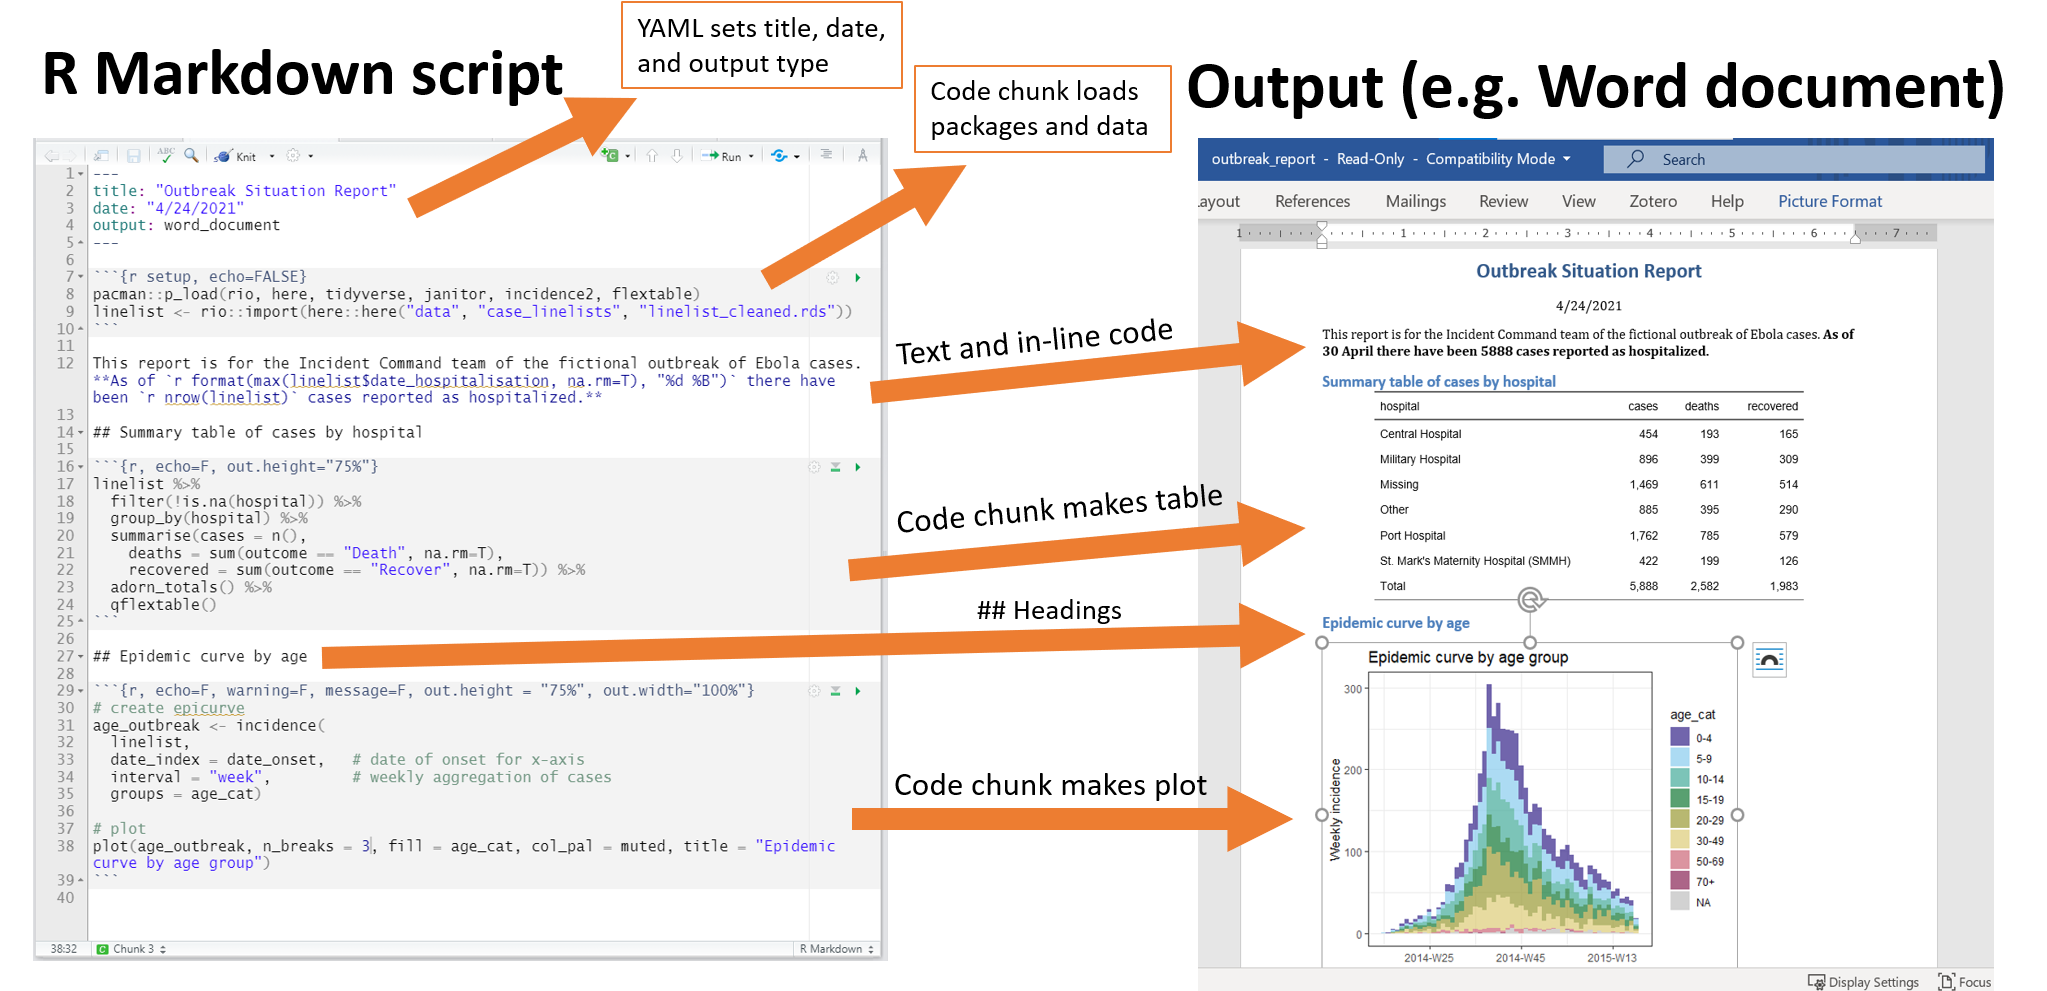
\includegraphics[width=1\linewidth]{images/rmarkdown_translation}

\hypertarget{yaml}{%
\subsection{YAML}\label{yaml}}

Referred to as the `YAML metadata' or just `YAML', this is at the top of the R Markdown document. This section of the script will tell your Rmd file \textbf{what type of output to produce}, formatting preferences, and other metadata such as document title, author, and date.
In the example above, because we clicked that our default output would be an html file, we can see that the YAML says output: \texttt{html\_document}. However we can also change this to say \texttt{powerpoint\_presentation} or \texttt{word\_document} or even \texttt{pdf\_document}.

\begin{rmdquestion}
Can you edit the YAML in the Rmarkdown file in the markdown folder to
have your name as author, today's date and the title of the file should
be called ``Darwin's Maize Plants''.
\end{rmdquestion}

\hypertarget{text}{%
\subsection{Text}\label{text}}

This is the narrative of your document, including the titles and headings. It is written in the ``markdown'' language, which is used across many different software.

Below are the core ways to write this text. See more extensive documentation available on R Markdown ``cheatsheets'' at the RStudio website\footnote{(\url{https://www.rstudio.com/resources/cheatsheets/})}.

\hypertarget{new-lines}{%
\subsubsection{New lines}\label{new-lines}}

Uniquely in R Markdown, to initiate a new line, enter *two spaces** at the end of the previous line and then Enter/Return.

\hypertarget{text-emphasis}{%
\subsubsection{Text emphasis}\label{text-emphasis}}

Surround your normal text with these characters to change how it appears in the output.

Underscores (\_text\_) or single asterisk (*text*) to \emph{italicise}

Double asterisks (**text**) for \textbf{bold} text

Back-ticks (`text`) to display text as \texttt{code}

The actual appearance of the font can be set by using specific templates (specified in the YAML metadata).

\hypertarget{titles-and-headings}{%
\subsubsection{Titles and headings}\label{titles-and-headings}}

A hash symbol in a text portion of a R Markdown script creates a heading. This is different than in a chunk of R code in the script, in which a hash symbol is a mechanism to comment/annotate/de-activate, as in a normal R script.

Different heading levels are established with different numbers of hash symbols at the start of a new line. One hash symbol is a title or primary heading. Two hash symbols are a second-level heading. Third- and fourth-level headings can be made with successively more hash symbols.

\begin{verbatim}
# First-level heading / title

## Second level heading  

### Third-level heading
\end{verbatim}

\hypertarget{bullets-and-numbering}{%
\subsubsection{Bullets and numbering}\label{bullets-and-numbering}}

Use asterisks (*) to created a bullets list. Finish the previous sentence, enter two spaces, Enter/Return twice, and then start your bullets. Include a space between the asterisk and your bullet text. After each bullet enter two spaces and then Enter/Return. Sub-bullets work the same way but are indented. Numbers work the same way but instead of an asterisk, write 1), 2), etc. Below is how your R Markdown script text might look.

Here are my bullets (there are two spaces after this colon):

\begin{verbatim}
* Bullet 1 (followed by two spaces and Enter/Return)  
* Bullet 2 (followed by two spaces and Enter/Return)  
  * Sub-bullet 1 (followed by two spaces and Enter/Return)  
  * Sub-bullet 2 (followed by two spaces and Enter/Return)  
\end{verbatim}

\hypertarget{code-chunks}{%
\subsection{Code Chunks}\label{code-chunks}}

Sections of the script that are dedicated to running R code are called ``chunks''. This is where you may load packages, import data, and perform the actual data management and visualisation. There may be many code chunks, so they can help you organize your R code into parts, perhaps interspersed with text. To note: These `chunks' will appear to have a slightly different background colour from the narrative part of the document.

Each chunk is opened with a line that starts with three back-ticks, and curly brackets that contain parameters for the chunk (\{ \}). The chunk ends with three more back-ticks.

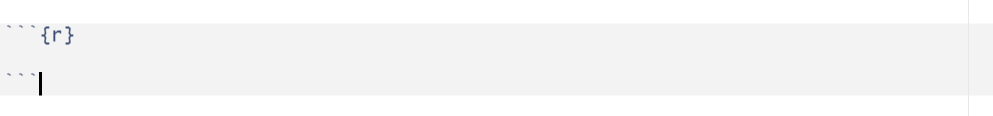
\includegraphics[width=0.8\linewidth]{images/chunk}

You can create a new chunk by typing it out yourself, by using the keyboard shortcut ``Ctrl + Alt + i'' (or Cmd + Shift + r in Mac), or by clicking the green `insert a new code chunk' icon at the top of your script editor.

Some notes about the contents of the curly brackets \{ \}:

They start with `r' to indicate that the language name within the chunk is R

After the r you can optionally write a chunk ``name'' -- these are not necessary but can help you organise your work. Note that if you name your chunks, you should ALWAYS use unique names or else R will \emph{complain} when you try to render.

The curly brackets can include other options too, written as tag=value, such as:

\begin{itemize}
\item
  eval = FALSE to not run the R code
\item
  echo = FALSE to not print the chunk's R source code in the output document
\item
  warning = FALSE to not print warnings produced by the R code
\item
  message = FALSE to not print any messages produced by the R code
\item
  include = either TRUE/FALSE whether to include chunk outputs (e.g.~plots) in the document
\item
  out.width = and out.height = - size of ouput e.g.~out.width = ``75\%''
\item
  fig.align = ``center'' adjust how a figure is aligned across the page
\item
  fig.show=`hold' if your chunk prints multiple figures and you want them printed next to each other (pair with out.width = c(``33\%'', ``67\%'').
\end{itemize}

A chunk header must be written in one line

Try to avoid periods, underscores, and spaces. Use hyphens ( - ) instead if you need a separator.

Read more extensively about the knitr options here\footnote{(\url{https://yihui.org/knitr/options/})}.

There are also two arrows at the top right of each chunk, which are useful to run code within a chunk, or all code in prior chunks. Hover over them to see what they do.

\hypertarget{here}{%
\subsection{Here}\label{here}}

The package \texttt{here} \citet{R-here} and its function \texttt{here()} make it easy to tell R where to find and to save your files - in essence, it builds file paths.

This is how \texttt{here()} works within an R project:

\begin{itemize}
\item
  When the here package is first loaded within the R project, it places a small file called ``.here'' in the root folder of your R project as a ``benchmark'' or ``anchor''
\item
  In your scripts, to reference a file in the R project's sub-folders, you use the function here() to build the file path in relation to that anchor
\item
  To build the file path, write the names of folders beyond the root, within quotes, separated by commas, finally ending with the file name and file extension as shown below
\item
  here() file paths can be used for both importing and exporting
\end{itemize}

So when you use here wrapped inside other functions for importing/exporting (like read\_csv or ggsave) if you include here you can still use the RProject location as the root directory when `knitting' Rmarkdown files, even if your markdown is tidied away into a separate markdown folder.

\begin{rmdquestion}
Can you take the code below and put it into an R code chunk?

Try your first ``knit'' to make a document.
\end{rmdquestion}

\begin{Shaded}
\begin{Highlighting}[]
\FunctionTok{library}\NormalTok{(here)}
\FunctionTok{library}\NormalTok{(tidyverse)}

\NormalTok{darwin }\OtherTok{\textless{}{-}} \FunctionTok{read\_csv}\NormalTok{(}\FunctionTok{here}\NormalTok{(}\StringTok{"data"}\NormalTok{, }\StringTok{"darwin.csv"}\NormalTok{))}
\NormalTok{darwin}
\end{Highlighting}
\end{Shaded}

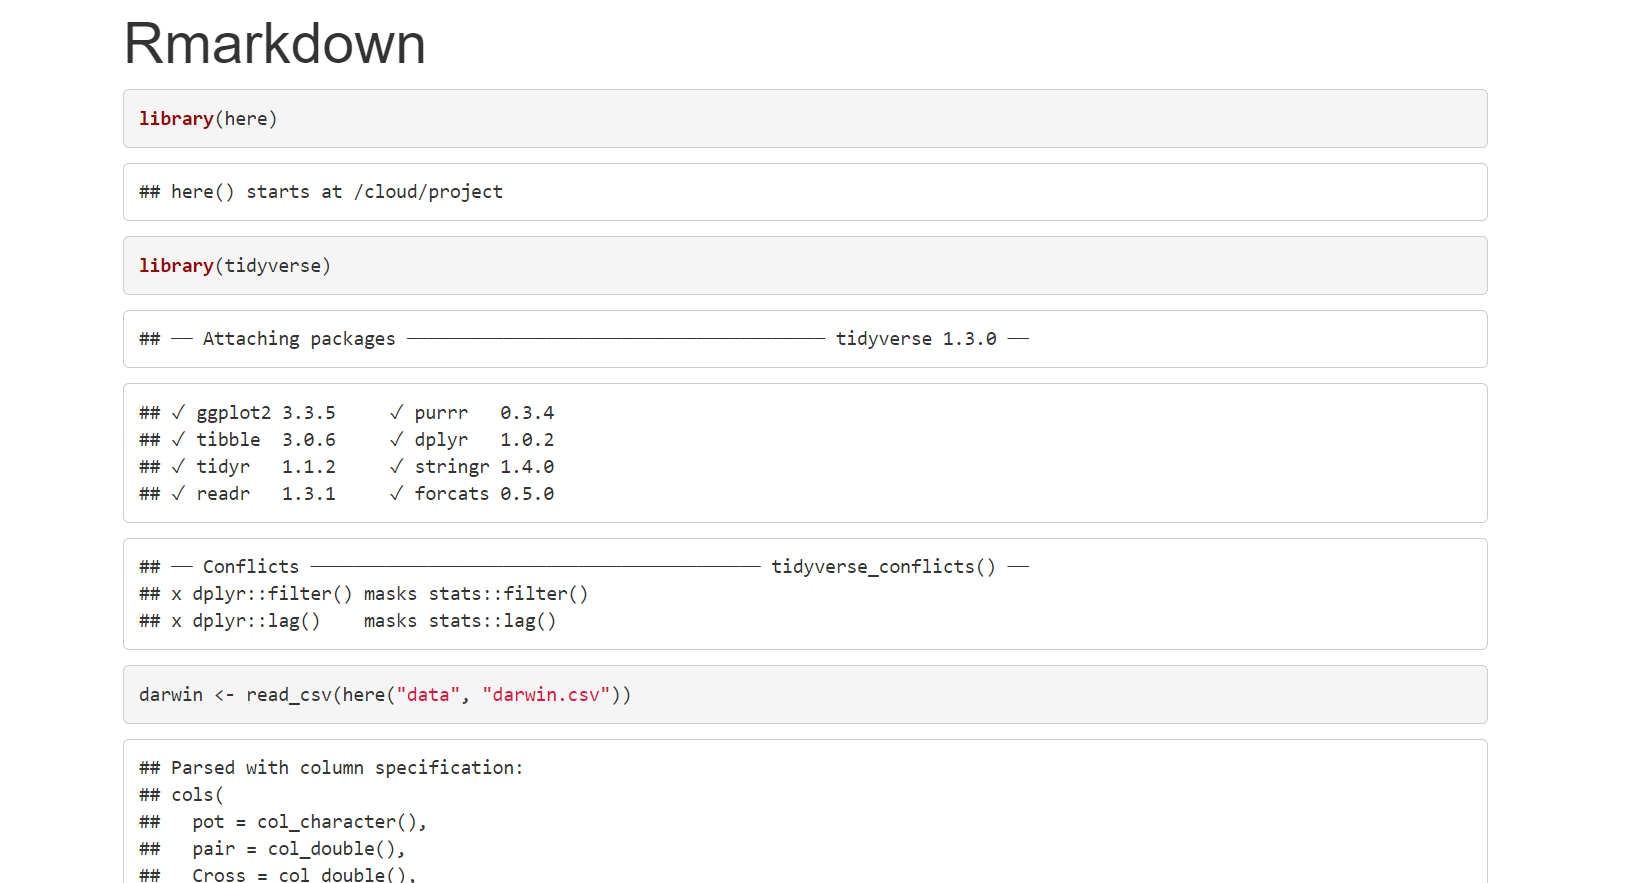
\includegraphics[width=1.2\linewidth]{images/markdown_output}

\begin{rmdquestion}
Hmmm looks a little messy.

Can you edit the R chunk so that the code and any warnings/messages are
invisible. But the code output is still printed?

Once you have made your edits try hitting `knit' again.
\end{rmdquestion}

\hypertarget{global-options}{%
\subsubsection{Global options}\label{global-options}}

For global options to be applied to all chunks in the script, you can set this up within your very first R code chunk in the script.
This is very handy if you know you will want the majority of your code chunks to behave in the same way.
For instance, so that only the outputs are shown for each code chunk and not the code itself, you can include this command in the R code chunk (and set this chunk to include=false):

\begin{Shaded}
\begin{Highlighting}[]
\NormalTok{knitr}\SpecialCharTok{::}\NormalTok{opts\_chunk}\SpecialCharTok{$}\FunctionTok{set}\NormalTok{(}\AttributeTok{echo =} \ConstantTok{FALSE}\NormalTok{) }
\end{Highlighting}
\end{Shaded}

\hypertarget{in-text-code}{%
\subsubsection{In-text code}\label{in-text-code}}

You can also include minimal R code within back-ticks. Within the back-ticks, begin the code with ``r'' and a space, so RStudio knows to evaluate the code as R code. See the example below.

` r Sys.Date()`

When typed in-line within a section of what would otherwise be Markdown text, it knows to produce an r output instead 2022-02-12

The example above is simple (showing the current date), but using the same syntax you can display values produced by more complex R code (e.g.~to calculate the min, median, max of a column). You can also integrate R objects or values that were created in R code chunks \emph{earlier} in the script.

\begin{Shaded}
\begin{Highlighting}[]
\NormalTok{average\_height }\OtherTok{\textless{}{-}}\NormalTok{ darwin }\SpecialCharTok{\%\textgreater{}\%} 
  \FunctionTok{summarise}\NormalTok{(}\AttributeTok{mean\_self=}\FunctionTok{mean}\NormalTok{(Self),}
            \AttributeTok{mean\_cross=}\FunctionTok{mean}\NormalTok{(Cross))}
\end{Highlighting}
\end{Shaded}

The average height of the self-crossed plants is ` r average\_height {[},1{]}`cm while the outcrossed plants are ` r average\_height {[},2{]}`cm, so on average the outcrossed plants are ` r average\_height {[},2{]}- average\_height {[},1{]}`cm taller.

\begin{rmdquestion}
Can you include the above code block and make sure it runs without the
code being visible? Underneath include the text - it should produce the
code outputs in the knitted doc. Try it!
\end{rmdquestion}

\hypertarget{images}{%
\section{Images}\label{images}}

You can include images in your R Markdown in several ways:

knitr::include\_graphics(``path/to/image.png'')

\begin{Shaded}
\begin{Highlighting}[]
\NormalTok{knitr}\SpecialCharTok{::}\FunctionTok{include\_graphics}\NormalTok{(}\StringTok{"../data/images/darwin.png"}\NormalTok{)}
\CommentTok{\# ../ is necessary here because in order to organise the file path starting in the markdown folder, directing it to go UP to the parent folder then down through data/images}
\end{Highlighting}
\end{Shaded}

Alternatively we could use the \texttt{here()} function - which means it doesn't matter where our markdown file `lives'.

knitr::include\_graphics(here::here(``path'', ``to'', ``image.png''))

\begin{Shaded}
\begin{Highlighting}[]
\NormalTok{knitr}\SpecialCharTok{::}\FunctionTok{include\_graphics}\NormalTok{(}\FunctionTok{here}\NormalTok{(}\StringTok{"data"}\NormalTok{, }\StringTok{"images"}\NormalTok{, }\StringTok{"darwin.png"}\NormalTok{))}
\end{Highlighting}
\end{Shaded}

\begin{rmdquestion}
Can you get your document to knit with this new image included?
\end{rmdquestion}

\hypertarget{tables}{%
\section{Tables}\label{tables}}

To create and manage able objects, we first pass the data frame through the \texttt{kable()} function. The package \texttt{kableExtra} \citet{R-kableExtra} gives us lots of extra styling options.\footnote{(\url{https://cran.r-project.org/web/packages/kableExtra/vignettes/awesome_table_in_html.html})}

\begin{rmdquestion}
Can you get this working? Add the library call for \texttt{kableExtra}
to the first chunk of your Rmd file, then make a chunk for the below at
the bottom of your file and hit knit to test.
\end{rmdquestion}

\begin{Shaded}
\begin{Highlighting}[]
\NormalTok{darwin }\SpecialCharTok{\%\textgreater{}\%} 
  \FunctionTok{summarise}\NormalTok{(}\AttributeTok{mean\_self=}\FunctionTok{mean}\NormalTok{(Self),}
            \AttributeTok{mean\_cross=}\FunctionTok{mean}\NormalTok{(Cross)) }\SpecialCharTok{\%\textgreater{}\%} 
  \FunctionTok{kbl}\NormalTok{(}\AttributeTok{caption=}\StringTok{"Table 1. example table caption"}\NormalTok{) }\SpecialCharTok{\%\textgreater{}\%} 
  \FunctionTok{kable\_styling}\NormalTok{(}\AttributeTok{bootstrap\_options =} \StringTok{"striped"}\NormalTok{, }\AttributeTok{full\_width =}\NormalTok{ F, }\AttributeTok{position =} \StringTok{"left"}\NormalTok{)}
\end{Highlighting}
\end{Shaded}

\hypertarget{self-contained-documents}{%
\section{Self-contained documents}\label{self-contained-documents}}

For a relatively simple report, you may elect to organize your R Markdown script such that it is ``self-contained'' and does not involve any external scripts.

Everything you need to run the R markdown is imported or created within the Rmd file, including all the code chunks and package loading. This ``self-contained'' approach is appropriate when you do not need to do much data processing (e.g.~it brings in a clean or semi-clean data file) and the rendering of the R Markdown will not take too long.

In this scenario, one logical organization of the R Markdown script might be:

\begin{itemize}
\item
  Set global knitr options
\item
  Load packages
\item
  Import data
\item
  Process data
\item
  Produce outputs (tables, plots, etc.)
\item
  Save outputs, \emph{if applicable} (.csv, .png, etc.)
\end{itemize}

\hypertarget{source-files}{%
\section{Source files}\label{source-files}}

One variation of the ``self-contained'' approach is to have R Markdown code chunks ``source'' (run) other R scripts.

This can make your R Markdown script less cluttered, more simple, and easier to organize. It can also help if you want to display final figures at the beginning of the report.

In this approach, the final R Markdown script simply combines pre-processed outputs into a document.

\begin{verbatim}
source(here("scripts", "your-script.R"))
\end{verbatim}

\begin{rmdquestion}
Can you try it for yourself? There is a pre-written script in your R
project, just use the source command to read in this script - then you
can call objects made externally - in this case a penguin plot - put the
code block in and hit knit.
\end{rmdquestion}

\begin{Shaded}
\begin{Highlighting}[]
\FunctionTok{source}\NormalTok{(}\FunctionTok{here}\NormalTok{(}\StringTok{"scripts"}\NormalTok{, }\StringTok{"penguin script.R"}\NormalTok{))}
\NormalTok{scat }\DocumentationTok{\#\#\# object generated in penguin script}
\end{Highlighting}
\end{Shaded}

\hypertarget{exercise---make-your-own-rmd-document}{%
\section{Exercise - Make your own Rmd document}\label{exercise---make-your-own-rmd-document}}

The data found in ``darwin.csv'' was originally collected by Charles Darwin and published in \emph{The effects of cross and self-fertilisation in the vegetable kingdom}, in 1876. In this publication he described how he produced seeds of \emph{Zea mays} (maize) that were fertilised with pollen from the same individual (inbreeding) or by crossing to a different plant (outbreeding). Pairs of seeds were then taken from self-fertilised and crossed plants and germinated in pots, and the height of the young seedlings measured as a proxy for their fitness. Darwin wanted to know whether inbreeding reduced their fitness.

\begin{rmdquestion}
Can you make your first reproducible document?
\end{rmdquestion}

\begin{itemize}
\item
  Write a short background on this subject 250-300 words on the data and the experimental hypothesis (use some of the information above)
\item
  Write a results section on this data including:

  \begin{itemize}
  \item
    A figure of the individual data points
  \item
    A summary results table with the mean and s.d. for the plants
  \item
    Write a summary of the results where the figures and table are referenced but you \emph{must} describe the results too. e.g.~
  \end{itemize}
\end{itemize}

``Results are shown in Figure 1'' is \textbf{not ok}

But \emph{in your own words} describe the direction and effect size of any differences and then refer to Figures and tables

``The mean height of self-crossed plants is \emph{x} and the mean height of crossed plants is \emph{y}, meaning on average self-crossed plants are\ldots{} which may indicate that \ldots{} (Figure 1, Table 1)''

\begin{itemize}
\tightlist
\item
  knit your rmarkdown as a \textbf{pdf} and submit to Blackboard.
\end{itemize}

\begin{rmdtip}
Remember your code blocks must be in the right order!!!
\end{rmdtip}

\hypertarget{summing-up-rmarkdown}{%
\section{Summing up Rmarkdown}\label{summing-up-rmarkdown}}

\hypertarget{what-we-learned-2}{%
\subsection{What we learned}\label{what-we-learned-2}}

You have learned

\begin{itemize}
\item
  How to use markdown
\item
  How to embed R chunks, to produce code, figures and analyses
\item
  How to organise projects with \texttt{here}
\item
  How to knit to pdf and html outputs
\item
  How to make simple tables
\end{itemize}

You have used

\begin{itemize}
\item
  \texttt{knitr} as part of Rmarkdown
\item
  \texttt{kableExtra} \citet{R-kableExtra}
\item
  \texttt{here} \citet{R-here}
\end{itemize}

\hypertarget{further-reading-guides-and-tips-1}{%
\subsection{Further Reading, Guides and tips}\label{further-reading-guides-and-tips-1}}

\href{https://www.rstudio.com/resources/cheatsheets/}{R Cheat Sheets}

\citet{xie2015} Dynamic documents with Rmarkdown

\emph{The fully comprehensive guide}

(\url{https://rmarkdown.rstudio.com/articles_intro.html})

(\url{https://rmarkdown.rstudio.com/authoring_quick_tour.html})

\hypertarget{version-control-with-github-week-six}{%
\chapter{Version control with GitHub: Week Six}\label{version-control-with-github-week-six}}

\hypertarget{lets-git-it-started}{%
\section{Let's Git it started}\label{lets-git-it-started}}

Git is a \textbf{version control system}. Originally built to help groups of developers work collaboratively on big software projects. It helps us manage our RStudio projects - with tracked changes.

Git and GitHub are a big part of the data science community. We can use GitHub in a number of ways

\begin{enumerate}
\def\labelenumi{\arabic{enumi})}
\item
  To source code and repurpose analyses built by others for our own uses
\item
  Manage our analysis projects so that all parts of it:
\end{enumerate}

\begin{itemize}
\item
  Data
\item
  Scripts
\item
  Figures
\item
  Reports
\end{itemize}

Are version controlled and open access

\begin{enumerate}
\def\labelenumi{\arabic{enumi})}
\setcounter{enumi}{2}
\item
  Version control lets you recover from any mistakes \& your analysis is \emph{backed up} externally
\item
  When you come to publish any reports - your analysis is accessible to others
\item
  Build up your own library of projects to show what you can do in Data Science
\end{enumerate}

Watch \href{https://www.youtube.com/watch?v=w3jLJU7DT5E}{this video} \emph{before} or \emph{after} today's session

\hypertarget{will-this-be-fun}{%
\subsection{Will this be fun?}\label{will-this-be-fun}}

No.

Using GitHub and version control is a bit like cleaning your teeth. It's not exactly fun, but it's good for you and it promotes excellent hygiene. It also only takes about 2 minutes.

When we talk a about projects on GitHub we refer to Repositories / repos.

Repos on GitHub are the same unit as an RStudio Project - it's a place where you can easily store all information/data/etc. related to whatever project you're working on.

The way in which we will set up our RStudio Projects will now have a few extra steps to it

\begin{itemize}
\item
  Make a new GitHub repository (or \emph{fork} an existing one)
\item
  Make a New project on RStudio Cloud - selecting the \emph{from GitHub Repository} option
\item
  Clone your GitHub repo into an RStudio Project
\item
  Make sure RStudio and Github can \emph{talk} to each other
\item
  Go about your normal business
\item
  When it comes to \emph{saving} your files, you will also periodically make a \textbf{commit} - this takes a multi-file \emph{snapshot} of your \emph{entire} project
\item
  At the end of a session \textbf{push} your changes to GitHub.
\end{itemize}

These changes to working with RStudio will feel a little different at first, but will quickly become routine - and are a big step forward in your Data Science skills.

\hypertarget{the-payoff}{%
\subsection{The Payoff}\label{the-payoff}}

\begin{itemize}
\item
  \textbf{A portfolio} build up a library of data science projects you can show off
\item
  \textbf{be keen} track the development of R packages on GitHUb
\item
  \textbf{version control} keep a safe archive of all your edits and changes
\item
  \textbf{play with others} easy ways to collaborate on data science projects
\end{itemize}

For the full rundown on how to use Git and R you can't go wrong with checking out \citet{happygit}

\hypertarget{set-up-github}{%
\section{Set up GitHub}\label{set-up-github}}

First things first you will need to set yourself up with a GitHub account.

Head to \href{https://github.com/}{GitHub} and sign up for a free account.

\begin{rmdwarning}
Make a careful note of

\begin{itemize}
\item
  The username you choose
\item
  Use the same email you have signed up to RStudio Cloud with
\item
  Note your password carefully!
\end{itemize}
\end{rmdwarning}

\hypertarget{exercise-1.-fork-clone-an-existing-repo-on-github-make-edits-push-back}{%
\section{\texorpdfstring{\textbf{Exercise 1.} Fork \& clone an existing repo on GitHub, make edits, push back}{Exercise 1. Fork \& clone an existing repo on GitHub, make edits, push back}}\label{exercise-1.-fork-clone-an-existing-repo-on-github-make-edits-push-back}}

\textbf{a.} Go to \href{https://github.com/}{github.com} and log in (you need your own account - for sign up with your uea.ac.uk e-mail)

\textbf{b.} In the Search bar, look for repo \textbf{Philip-Leftwich/5023Y-Happy-Git}

\textbf{c.} Click on the repo name, and look at the existing repo structure

\textbf{d.} \textbf{FORK} the repo

\hypertarget{what-the-hell-is-a-fork}{%
\subsection{What the hell is a fork?}\label{what-the-hell-is-a-fork}}

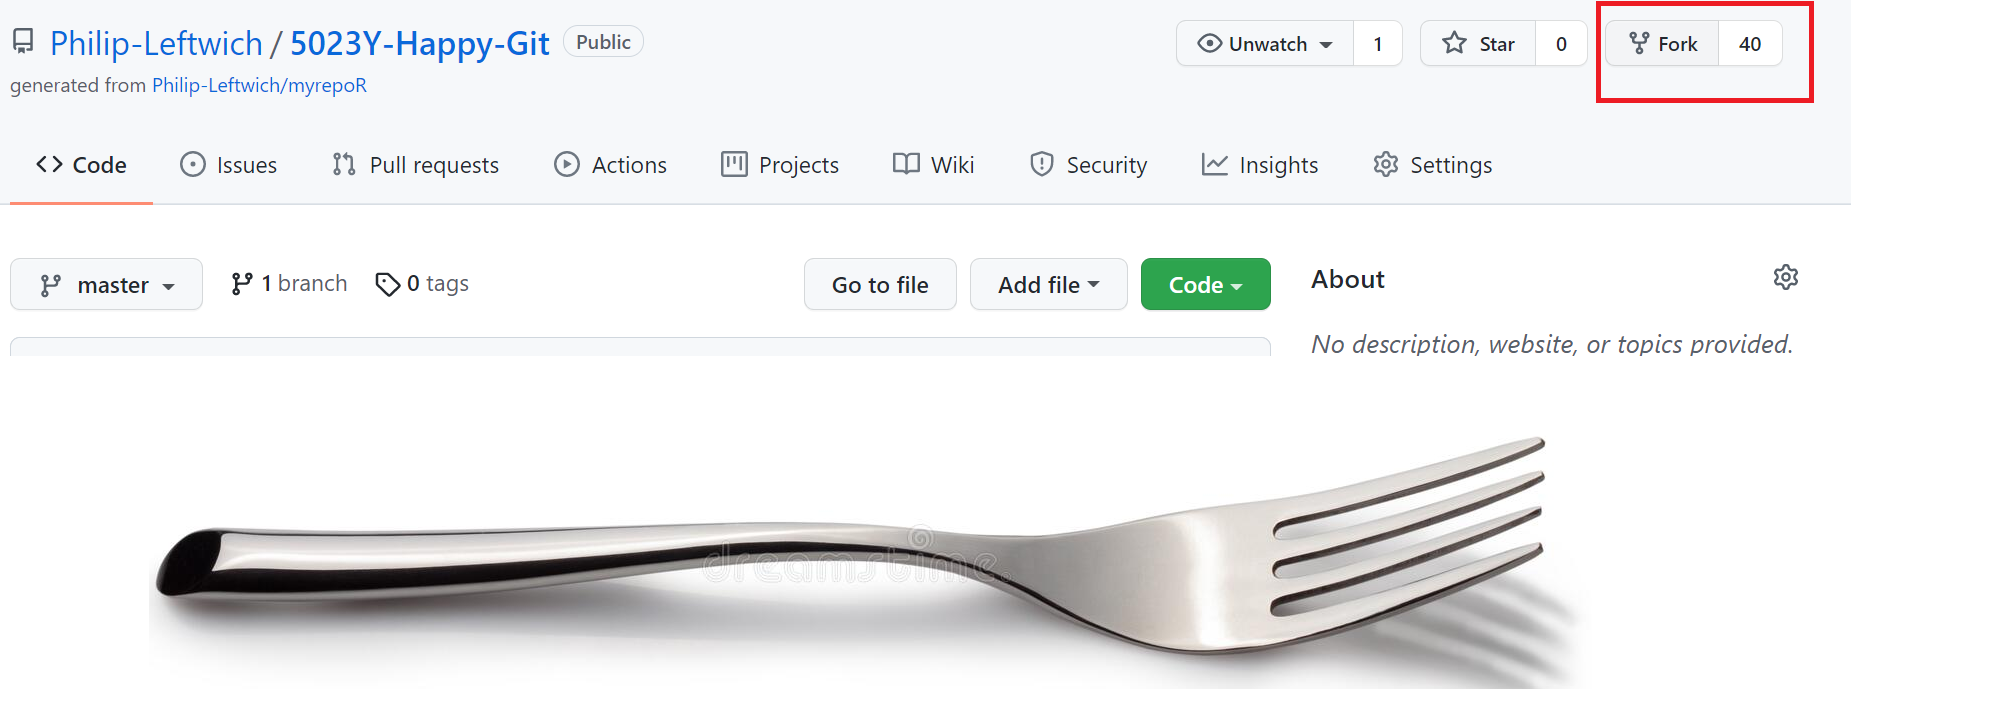
\includegraphics[width=27.68in]{images/fork}

A fork is when you generate a \emph{personal} copy of another user's repository (\ref{glossary-github}).

\textbf{e.} Press Clone/download and copy the URL, then create a \textbf{new} project in RStudio Cloud selecting the \textbf{New project from Git repository} option - make sure you are in the 5023Y Workspace

\includegraphics[width=25.46in]{images/new-project}

\textbf{f.} Open the some\_cool\_animals.Rmd document, and the accompanying html

\textbf{g.} Add \emph{your name} to the top of the document

\textbf{h.} BUT WAIT. We have forgotten to add a great image and facts about a very important species - Baby Yoda, including an image (the file is in the repo, and the info to add is below).

\textbf{FACTS}

\includegraphics[width=16.25in]{images/Grogu}

\begin{itemize}
\item
  Also known as ``The Child''
\item
  likes unfertilised frog eggs \& control knobs
\item
  strong with the force
\end{itemize}

~

~

\textbf{i.} Once you've added Grogu, knit the Rmd document to update the html

\textbf{j.} Add your Git credentials go to section (\ref{talking-to-github})

\textbf{k.} Stage, Commit \& Push all files (\ref{glossary-github})

Staged - pick those files which you intend to bind to a commit

Commit - write a short descriptive message, binds changes to a single commit (\ref{commit})

Push - ``Pushes'' your changes from the local repo to the remote repo on GitHub (\ref{push})

\textbf{l.} On GitHub, refresh and see that files are updated. Cool! Now you've used something someone else has created, customized it, and saved your updated version.

\hypertarget{talking-to-github}{%
\section{Talking to GitHub}\label{talking-to-github}}

Getting set up to talk to GitHub can seem like a pain. Eventually when you work on your own computer - with a copy of R \& RStudio installed - you will only have to do this once. For now when we use RStudio Cloud - it looks like we have to do this \textbf{once per project}. It only takes a few seconds and you should put these commands \textbf{directly into your console}.

Run this first line \textbf{in your console} and put in your GitHub username and the e-mail connected to your GitHub account.

\begin{quote}
**Note - you might not have to do this first step if you go to your RStudio Cloud profile \textgreater{} Authentication and select Github Enabled \& Private repo access also enabled
\end{quote}

\begin{Shaded}
\begin{Highlighting}[]
\NormalTok{usethis}\SpecialCharTok{::}\FunctionTok{use\_git\_config}\NormalTok{(}\AttributeTok{user.name =} \StringTok{"Jane Doe"}\NormalTok{, }\AttributeTok{user.email =} \StringTok{"jane@example.org"}\NormalTok{)}
\end{Highlighting}
\end{Shaded}

Then you need to give RStudio Cloud your GitHub Personal Access Token, which you can retrieve by going to Settings \textgreater{} Develope Settings \textgreater{} Generate Token (\ref{glossary-github})

Select all the ``scopes'' and name your token.

\includegraphics[width=25.19in]{images/git-PAT}

Make a note of this because you will need it whenever you set up a new project you want to talk to GitHub. GitHub recently removed password authentication in favour of PATs, but RStudio Cloud doesn't seem to have updated this yet - that's ok though - just enter this line of code - then copy+paste your PAT when prompted. - Option set/replace these credentials.

\begin{Shaded}
\begin{Highlighting}[]
\NormalTok{gitcreds}\SpecialCharTok{::}\FunctionTok{gitcreds\_set}\NormalTok{()}
\end{Highlighting}
\end{Shaded}

If you forget your PAT - that's ok - you can't retrieve it - but you can just generate a new one.

\hypertarget{see-changes}{%
\subsection{See changes}\label{see-changes}}

The first and most immediate benefit of using GitHub with your RStudio Project is seeing the changes you have made since your last commit.

The RStudio Git pane lists every file that's been added, modified or deleted. The icon describes the change:

\begin{itemize}
\item
  \includegraphics[width=0.53in]{images/git-modified} You've changed a file
\item
  \includegraphics[width=0.56in]{images/git-unknown} You've added a new file Git hasn't seen before
\item
  \includegraphics[width=0.58in]{images/git-deleted} You've deleted a file
\end{itemize}

You can get more details on the changes that have been made to each file by right-clicking and selecting diff
\includegraphics[width=1.28in]{images/git-diff} . This opens a new window highlighting the \textbf{diff}erences between your current file and the previous commit.

\includegraphics[width=18.61in]{images/git-diff-window}
The background colours tells you whether the text has been added (green) or removed (red). (If you're colourblind you can use the line numbers in the two columns at the far left as a guide).

\hypertarget{how-to-use-version-control---when-to-commit-push-and-pull}{%
\section{How to use version control - when to commit, push and pull}\label{how-to-use-version-control---when-to-commit-push-and-pull}}

Repositories (repos) on GitHub are the same unit as an RStudio Project - it's a place where you can easily store all information/data/etc. related to whatever project you're working on.

When we create a Repository in GitHub and have it communicating with a Project in RStudio, then we can get (\textbf{pull}) information from GitHub to RStudio, or \textbf{push} information from RStudio to GitHub where it is safely stored and/or our collaborators can access it. It also keeps a \emph{complete history} of updated versions that can be accessed/reviewed by you and your collaborators at any time, from anywhere, as long as you have the internet.

I have mentioned the term \textbf{commit} a few times (\ref{glossary-github}). The fundamental unit of work in Git is a commit. A commit takes a snapshot of your code at a specified point in time.

You create a commit in two stages:

\begin{enumerate}
\def\labelenumi{\arabic{enumi}.}
\item
  You \textbf{stage} files, telling Git which changes should be included in the next commit.
\item
  You \textbf{commit} the staged files, describing the changes with a message.
\end{enumerate}

To create a new commit, \textbf{save} your files, then select files for inclusion by \emph{staging} them, tick the checkbox and then select the commit box

\includegraphics[width=11in]{images/stage_step_4}

A new window will open - and you will see the diffs in the bottom pane, and all the files you have selected for the latest commit.

\hypertarget{commit}{%
\subsection{Commit}\label{commit}}

You now need to write a \textbf{commit message}. This should be short but meaningful

\includegraphics[width=17.38in]{images/stage_step_5}

Describe the \textbf{why}, not the what. Git stores all the associated differences between commits, the message doesn't need to say exactly what changed. Instead it should provide a summary that focuses on the \textbf{reasons} for the change. Make this understandable for someone else!

Once you click commit a new window will open that summarises your commit - and you can close this

\includegraphics[width=17.36in]{images/stage_step_6}

\hypertarget{push}{%
\subsection{Push}\label{push}}

At the moment, all of your commits are \emph{local}, in order to send them to GitHub you have to select \textbf{Push} at this point your github credentials need to be in place - if you get prompted to provide these, close the windows and follow the steps here (\ref{talking-to-github}) before trying again.

Your git pane will be empty at this point - but there is a little message at the top detailing how many commits you are \emph{ahead} of the master repo on GitHub.

\includegraphics[width=26.65in]{images/stage_step_7}

\hypertarget{a-couple-of-general-tips}{%
\subsection{A couple of general tips:}\label{a-couple-of-general-tips}}

\begin{rmdnote}
\begin{itemize}
\item
  Pull at the start of \textbf{every session} this retrieves the master
  repo from GitHub - which you update at the end of every session. This
  helps prevent \emph{conflicts}
\item
  \textbf{Commit/push} in small, meaningful increments and do this
  often. You can make \textbf{multiple} commits in a session - and
  \textbf{always push at the end of the session}
\item
  In this way your GitHub Repo becomes the \textbf{master copy} of your
  project.
\end{itemize}
\end{rmdnote}

\hypertarget{turn-back-time-with-git}{%
\subsection{Turn back time with Git}\label{turn-back-time-with-git}}

"If I could turn back time,

If I could find a way,

I'd take back those commits that have hurt you,

And you'd stay" - Cher

Once you start using Git with RStudio - you get a whole bunch of different options for undoing changes, correcting mistakes and turning back time to previous versions!

\begin{itemize}
\item
  To undo changes between commits you can select the diff option and remove lines one-by-one
\item
  Right-click on a file in the Git pane and select the revert option will undo all changes between this and the previous commit \textbf{beware} cannot be undone.
\end{itemize}

If you don't catch a mistake right away you can select the history button
\includegraphics[width=0.56in]{images/git-history} and \textbf{pull} previous commits from GitHub

\hypertarget{exercise-2.-github-classrooms-enabled-r-projects-with-subfolders}{%
\section{\texorpdfstring{\textbf{Exercise 2.} GitHub Classrooms enabled R Projects with subfolders}{Exercise 2. GitHub Classrooms enabled R Projects with subfolders}}\label{exercise-2.-github-classrooms-enabled-r-projects-with-subfolders}}

GitHub Classrooms is a way for me to set repos as assigments - when you accept an assignment on GitHub Classroom it \emph{automatically} forks a private repo for you.

You should make regular commits and pushes to save your work as you go - and I will be grading your project repositories on GitHub classrooms when you do your assignment work.

\begin{rmdwarning}
When you accept an assignment on GitHub classrooms - the repo won't
appear on your main profile, this is because it belongs to our class
rather than you. You can always find it by searching through your
Organisations - \textbf{but} it's probably easiest just to make a
bookmark/make a note of your unique URL for each assignment.
\end{rmdwarning}

\textbf{a.} Follow this \href{https://classroom.github.com/a/QFt76-i2}{invite link}

\textbf{b.} You will be invited to sign-in to Github (if not already) \& to join the UEABIO organisation

\textbf{c.} Clone your assignment to work locally in RStudio Cloud - 5023Y Workspace

\textbf{d.} In your local project folder, create subfolders `data' and `figures', `scripts', `markdown' (\textbf{Note} use the dir.create commands in the console)

\textbf{e.} Drop the file disease\_burden.csv into the `data' subfolder

\textbf{f.} Open a new .R script

\textbf{g.} Attach the \texttt{tidyverse}, \texttt{janitor}, and optionally \texttt{here} packages

\textbf{h.} Read in the infant\_mortality.csv data

This is a file look at the death rate for every country in the world across six decades. See the README for more information

\textbf{i.} Stage, commit \& push at this point - notice that the empty folder `final\_graphs' doesn't show up (won't commit an empty folder) - \textbf{you will have to set up your git credentials again}

\textbf{j.} Back in the script, write a short script to read and clean the data.

This script is pre-written, it puts the data in tidy format, cleans names, makes sure year is treated as date data and filters four countries of interest.

Assign this to a new object

\begin{Shaded}
\begin{Highlighting}[]
\FunctionTok{library}\NormalTok{(tidyverse)}
\FunctionTok{library}\NormalTok{(lubridate)}
\FunctionTok{library}\NormalTok{(janitor)}
\FunctionTok{library}\NormalTok{(plotly)}

\NormalTok{infant\_mortality }\OtherTok{\textless{}{-}} \FunctionTok{read\_csv}\NormalTok{(}\StringTok{"data/infant\_mortality.csv"}\NormalTok{) }

\NormalTok{subset\_infant\_mortality }\OtherTok{\textless{}{-}}\NormalTok{ infant\_mortality }\SpecialCharTok{\%\textgreater{}\%}
  \FunctionTok{pivot\_longer}\NormalTok{(}\AttributeTok{cols=}\StringTok{"1960"}\SpecialCharTok{:}\StringTok{"2020"}\NormalTok{, }
               \AttributeTok{names\_to=}\StringTok{"year"}\NormalTok{,               }
               \AttributeTok{values\_to=}\StringTok{"infant\_mortality\_rate"}\NormalTok{) }\SpecialCharTok{\%\textgreater{}\%}
  \FunctionTok{mutate}\NormalTok{(}\AttributeTok{year=}\NormalTok{lubridate}\SpecialCharTok{::}\FunctionTok{years}\NormalTok{(year)) }\SpecialCharTok{\%\textgreater{}\%} \CommentTok{\# set ymd format}
  \FunctionTok{mutate}\NormalTok{(}\AttributeTok{year=}\NormalTok{lubridate}\SpecialCharTok{::}\FunctionTok{year}\NormalTok{(year)) }\SpecialCharTok{\%\textgreater{}\%} \CommentTok{\# extract year}
\NormalTok{  janitor}\SpecialCharTok{::}\FunctionTok{clean\_names}\NormalTok{() }\SpecialCharTok{\%\textgreater{}\%} \CommentTok{\# put names in snake case}
  \FunctionTok{filter}\NormalTok{(country\_name }\SpecialCharTok{\%in\%} 
           \FunctionTok{c}\NormalTok{(}\StringTok{"United States"}\NormalTok{, }
             \StringTok{"Japan"}\NormalTok{, }
             \StringTok{"Afghanistan"}\NormalTok{, }
             \StringTok{"United Kingdom"}\NormalTok{)) }\CommentTok{\# extract four countries}

\CommentTok{\# View(subset\_infant\_mortality)}

\CommentTok{\# subset the date according to (US,UK, Japan = lowest infant death rates, Afghanistan = highest infant death rates)}
\end{Highlighting}
\end{Shaded}

\textbf{k.} Make a ggplot plotting the infant mortality rate by country

HINT - use \texttt{geom\_line()} and remember to separate countries by colour

\begin{Shaded}
\begin{Highlighting}[]
\FunctionTok{ggplot}\NormalTok{(}\AttributeTok{data =}\NormalTok{ subset\_infant\_mortality) }\SpecialCharTok{+}
  \FunctionTok{geom\_line}\NormalTok{(}\FunctionTok{aes}\NormalTok{(}\AttributeTok{x =}\NormalTok{ year,}
                 \AttributeTok{y =}\NormalTok{ infant\_mortality\_rate,}
                 \AttributeTok{color =}\NormalTok{ country\_name))}
\end{Highlighting}
\end{Shaded}

\textbf{l.} Update your graph with direct labels (using \texttt{annotate}) and vertical or horizontal lines with \texttt{geom\_vline} or \texttt{geom\_hline}.

\includegraphics{bookdown-demo_files/figure-latex/unnamed-chunk-221-1.pdf}

\textbf{m.} Use ggsave() to write your graph to a .png in the `final\_graphs' subfolder

\begin{Shaded}
\begin{Highlighting}[]
\FunctionTok{ggsave}\NormalTok{(}\StringTok{"figures/infant mortality graph.png"}\NormalTok{, }\AttributeTok{plot=}\NormalTok{mortality\_figure, }\AttributeTok{dpi=}\DecValTok{900}\NormalTok{, }\AttributeTok{width =} \DecValTok{7}\NormalTok{, }\AttributeTok{height =} \DecValTok{7}\NormalTok{)}
\end{Highlighting}
\end{Shaded}

\textbf{n.} Save, stage, commit

\textbf{o} Let's do one more cool and fun thing! And make an interactive version of our plot using plotly \citet{R-plotly} just for fun!

\begin{Shaded}
\begin{Highlighting}[]
\FunctionTok{ggplotly}\NormalTok{(mortality\_figure, }\AttributeTok{tooltip =} \FunctionTok{c}\NormalTok{(}\StringTok{"infant\_mortality\_rate"}\NormalTok{))}
\DocumentationTok{\#\# uses plotly package}
\end{Highlighting}
\end{Shaded}

\textbf{p} Now save, stage, commit \& \textbf{push}

\textbf{q.} Check that changes are stored on GitHub

(\textbf{NOTE} this will be in your organisations rather than repos)

\textbf{Make sure you finish both exercises before next week to become a GitHub pro!!!!!!!!!}

\hypertarget{find-your-classroom-repos}{%
\section{Find your classroom repos}\label{find-your-classroom-repos}}

When you work with GitHub classrooms your repos become part of our organisation UEABIO.
If you want to find your repos on GitHub then you can use the direct URL (if you noted it), or head to (\url{https://github.com/UEABIO}) - you should only be able to see repos that belong to \textbf{you}.

\includegraphics[width=18.83in]{images/classroom-organisation}

\hypertarget{glossary-github}{%
\section{Glossary-GitHub}\label{glossary-github}}

\begin{tabular}[t]{l|l}
\hline
Terms & Description\\
\hline
clone & A clone is a copy of a repository that lives on your computer instead of on a website's server somewhere, or the act of making that copy. When you make a clone, you can edit the files in your preferred editor and use Git to keep track of your changes without having to be online. The repository you cloned is still connected to the remote version so that you can push your local changes to the remote to keep them synced when you're online.\\
\hline
commit & A commit, or revision, is an individual change to a file (or set of files). When you make a commit to save your work, Git creates a unique ID that allows you to keep record of the specific changes committed along with who made them and when. Commits usually contain a commit message which is a brief description of what changes were made.\\
\hline
commit message & Short, descriptive text that accompanies a commit and communicates the change the commit is introducing.\\
\hline
fork & A fork is a personal copy of another user's repository that lives on your account. Forks allow you to freely make changes to a project without affecting the original upstream repository. You can also open a pull request in the upstream repository and keep your fork synced with the latest changes since both repositories are still connected.\\
\hline
Git & Git is an open source program for tracking changes in text files. It was written by the author of the Linux operating system, and is the core technology that GitHub, the social and user interface, is built on top of.\\
\hline
GitHub Classroom & GitHub Classroom automates repository creation and access control, making it easy to distribute starter code and collect assignments on GitHub\\
\hline
Markdown & Markdown is an incredibly simple semantic file format, not too dissimilar from .doc, .rtf and .txt. Markdown makes it easy for even those without a web-publishing background to write prose (including with links, lists, bullets, etc.) and have it displayed like a website.\\
\hline
pull & Pull refers to when you are fetching in changes and merging them. For instance, if someone has edited the remote file you're both working on, you'll want to pull in those changes to your local copy so that it's up to date\\
\hline
push & To push means to send your committed changes to a remote repository on GitHub.com. For instance, if you change something locally, you can push those changes so that others may access them.\\
\hline
README & A text file containing information about the files in a repository that is typically the first file a visitor to your repository will see. A README file, along with a repository license, contribution guidelines, and a code of conduct, helps you share expectations and manage contributions to your project.\\
\hline
repository & A repository (repo) is the most basic element of GitHub. They're easiest to imagine as a project's folder. A repository contains all of the project files (including documentation), and stores each file's revision history. Repositories can have multiple collaborators and can be either public or private.\\
\hline
RMarkdown & Rmarkdown is a package and filetype that are deeply embedded with RStudio to allow the integration of Markdown and output chunks of programming code (such as R) to publish a variety of different file types\\
\hline
personal access token & A token that is used in place of a password when performing Git operations over HTTPS. Also called a PAT.\\
\hline
\end{tabular}

\hypertarget{summing-up-github}{%
\section{Summing up GitHub}\label{summing-up-github}}

\hypertarget{what-we-learned-3}{%
\subsection{What we learned}\label{what-we-learned-3}}

You have learned

\begin{itemize}
\item
  How to fork and clone GitHub Projects
\item
  How to use GitHub classrooms
\item
  How to make RStudio and GitHub talk to each other
\item
  How to use version control, with stage, commit and push
\end{itemize}

You have used

\begin{itemize}
\item
  \texttt{gitcreds} \citet{R-gitcreds}
\item
  \texttt{usethis} \citet{R-usethis}
\end{itemize}

\hypertarget{further-reading-guides-and-tips-2}{%
\subsection{Further Reading, Guides and tips}\label{further-reading-guides-and-tips-2}}

\citet{happygit} \url{https://happygitwithr.com/}

\emph{The definitive guide}

\hypertarget{dealing-with-data-dplyr-week-eight}{%
\chapter{Dealing with data: dplyr: Week Eight}\label{dealing-with-data-dplyr-week-eight}}

\hypertarget{lets-get-going}{%
\section{Let's get going}\label{lets-get-going}}

You need to accept the latest assignment from \href{https://classroom.github.com/a/ifsL9ZE1}{Github Classrooms}.

We will be using this project until the end of term, so make sure you make regular commits, and push your work at the end of each session.

\hypertarget{introduction-to-dplyr}{%
\section{Introduction to dplyr}\label{introduction-to-dplyr}}

In chapters 3 and 4 we demonstrated a brief data analysis on the \texttt{palmerpenguins} dataset. We ran through several pipelines, but without going into huge amounts of detail on each section.

In this chapter we are going to get really well acquainted with \textbf{dplyr} \citet{R-dplyr}.

We will look at several core functions:

\begin{itemize}
\item
  \texttt{select} (get some columns)
\item
  \texttt{filter} (get some rows)
\item
  \texttt{arrange} (order the rows)
\item
  \texttt{mutate} (make new columns)
\item
  \texttt{group\_by} (add grouping information)
\item
  \texttt{summarise} (calculate summary information)
\end{itemize}

You should make careful notes about these functions and what they do. Build scripts with carefully added notes that you can use for future work

As you work through this (and other chapters) - make notes, if you take a break, set up a commit, or reach the end of a session - push your work to Github.

Make sure you are using the \href{https://www.rstudio.com/resources/cheatsheets/}{R Cheat Sheets for dplyr}

\hypertarget{select}{%
\section{select}\label{select}}

Start by setting up the packages you will need for this session

\begin{Shaded}
\begin{Highlighting}[]
\FunctionTok{library}\NormalTok{(tidyverse)}
\FunctionTok{library}\NormalTok{(lubridate)}

\NormalTok{penguins }\OtherTok{\textless{}{-}} \FunctionTok{read\_csv}\NormalTok{(}\StringTok{"data/penguins\_simple.csv"}\NormalTok{)}
\end{Highlighting}
\end{Shaded}

\begin{quote}
** Note - if you don't have these packages available, then you will need to run \texttt{install.packages("tidyverse")} - you should do this in the \emph{console} and \textbf{not} your script.
\end{quote}

We use select to \emph{select variables} from a dataframe or tibble. for example:

\begin{verbatim}
data_set %>% 
  select(variable_1, variable_2)
\end{verbatim}

\begin{quote}
** Note this is \emph{pseudocode} an example, not something you should run.
\end{quote}

\begin{itemize}
\item
  The data is piped into the first argument position of the \texttt{select} function
\item
  We then include the arguments where each one is the name of a variable in the dataset
\end{itemize}

For example if we actually run this:

\begin{Shaded}
\begin{Highlighting}[]
\NormalTok{penguins }\SpecialCharTok{\%\textgreater{}\%} 
  \FunctionTok{select}\NormalTok{(flipper\_length\_mm)}
\end{Highlighting}
\end{Shaded}

To look at flipper length - we should note a couple of things.

\begin{itemize}
\item
  Variable name is \textbf{not} in quotes
\item
  The original data is unchanged e.g.~penguins. Unless we assign the results of \texttt{select} with the assignment arrow (\textless-), the results will just be printed in the console
\item
  The order you ask for the variables in \texttt{select} determines the order of the columns in any new dataset
\item
  \texttt{select} returns a tibble
\item
  If we want to keep most variables, but \emph{remove one}, use the minus operator
\end{itemize}

\begin{Shaded}
\begin{Highlighting}[]
\NormalTok{penguins }\OtherTok{\textless{}{-}}\NormalTok{ penguins }\SpecialCharTok{\%\textgreater{}\%} 
  \FunctionTok{select}\NormalTok{(}\SpecialCharTok{{-}}\NormalTok{flipper\_length\_mm)}
\end{Highlighting}
\end{Shaded}

\begin{rmdwarning}
In the above option we just \emph{overwrote} the penguin dataset with a
new version that \emph{does not} contain flipper length. Be careful -
the above code will thrown an error message if you try to run it again
(there is no longer a flipper length variable to remove). If you want to
\emph{undo} this, the easiest way is to re-run your script to just
before this line.
\end{rmdwarning}

You can also use select to keep sets of consecutive variables together

\begin{Shaded}
\begin{Highlighting}[]
\NormalTok{penguins }\SpecialCharTok{\%\textgreater{}\%} 
  \FunctionTok{select}\NormalTok{(species}\SpecialCharTok{:}\NormalTok{flipper\_length\_mm)}
\end{Highlighting}
\end{Shaded}

There are also a number of helper functions like \texttt{starts\_with}, \texttt{ends\_with}, \texttt{contains}, \texttt{matches}. So if we want to keep all the variables that start with ``b''

\begin{Shaded}
\begin{Highlighting}[]
\NormalTok{penguins }\SpecialCharTok{\%\textgreater{}\%} 
  \FunctionTok{select}\NormalTok{(}\FunctionTok{starts\_with}\NormalTok{(}\StringTok{"b"}\NormalTok{))}
\end{Highlighting}
\end{Shaded}

\hypertarget{mutate}{%
\section{mutate}\label{mutate}}

Adding or creating new variables is a common task, we might want to make a log-transformation, subtract one value from another or use \texttt{mutate} to add a new date variable

\begin{Shaded}
\begin{Highlighting}[]
\NormalTok{penguins }\OtherTok{\textless{}{-}}\NormalTok{ penguins }\SpecialCharTok{\%\textgreater{}\%} 
  \FunctionTok{mutate}\NormalTok{(}\AttributeTok{date\_proper=}\FunctionTok{dmy}\NormalTok{(date))}
\end{Highlighting}
\end{Shaded}

Sometimes we want to change the values being used. For example we might want to change ``male'' and ``female'' to some abbreviation like ``M'' and ``F''. (Probably not, but it's an example!).

\begin{Shaded}
\begin{Highlighting}[]
\NormalTok{  penguins }\SpecialCharTok{\%\textgreater{}\%} 
  \FunctionTok{mutate}\NormalTok{(}\AttributeTok{sex=}\FunctionTok{case\_when}\NormalTok{(sex }\SpecialCharTok{==} \StringTok{"male"} \SpecialCharTok{\textasciitilde{}} \StringTok{"M"}\NormalTok{,}
\NormalTok{                       sex }\SpecialCharTok{==} \StringTok{"female"} \SpecialCharTok{\textasciitilde{}} \StringTok{"F"}\NormalTok{))}
\end{Highlighting}
\end{Shaded}

Things to know about \texttt{mutate}:

\begin{itemize}
\item
  Unless we assign the results of \texttt{mutate} back to an object (\textless-) the changes won't be saved
\item
  We can use newly created variables in further calculations \emph{within} the same \texttt{mutate}
\end{itemize}

\hypertarget{filter}{%
\section{filter}\label{filter}}

\texttt{filter} is used to subset observations in a dataframe. We might want to see the observations where \texttt{flipper\_length\_mm} is larger or smaller than a fixed value. Or we might want to only see the data from female penguins, or a particular species.

\begin{Shaded}
\begin{Highlighting}[]
\NormalTok{penguins }\SpecialCharTok{\%\textgreater{}\%} 
  \FunctionTok{filter}\NormalTok{(sex }\SpecialCharTok{==} \StringTok{"female"}\NormalTok{,}
\NormalTok{         species }\SpecialCharTok{==} \StringTok{"Adelie"}\NormalTok{,}
\NormalTok{         flipper\_length\_mm }\SpecialCharTok{\textless{}} \DecValTok{180}\NormalTok{)}
\end{Highlighting}
\end{Shaded}

In this example we've created a subset of \texttt{penguins} that only includes the five observations where flipper length is less than 180mm in female, Adelie penguins.

We can also set an either/or filter, for example if we only want small \& large flipper lengths.

\begin{Shaded}
\begin{Highlighting}[]
\NormalTok{penguins }\SpecialCharTok{\%\textgreater{}\%} 
  \FunctionTok{filter}\NormalTok{(species }\SpecialCharTok{==} \StringTok{"Adelie"}\NormalTok{, }
\NormalTok{         flipper\_length\_mm }\SpecialCharTok{\textless{}}\DecValTok{180} \SpecialCharTok{|} 
\NormalTok{           flipper\_length\_mm }\SpecialCharTok{\textgreater{}}\DecValTok{200}\NormalTok{)}
\end{Highlighting}
\end{Shaded}

This creates a subset of Adelie penguins, that only includes 14 observations where flipper length is less than 180mm or greater than 200mm.

The vertical bar \textbar{} is understood by R as OR.

The alternative is to look at values \emph{between} two amounts

\begin{Shaded}
\begin{Highlighting}[]
\NormalTok{penguins }\SpecialCharTok{\%\textgreater{}\%} 
  \FunctionTok{filter}\NormalTok{(species }\SpecialCharTok{==} \StringTok{"Adelie"}\NormalTok{,}
         \FunctionTok{between}\NormalTok{(flipper\_length\_mm, }\DecValTok{180}\NormalTok{,}\DecValTok{200}\NormalTok{))}
\end{Highlighting}
\end{Shaded}

\hypertarget{arrange}{%
\section{arrange}\label{arrange}}

We use arrange to reorder the rows of our data. Instances where we `need' to do this are rare. But we may often want to reorder rows so that we can understand the data more easily

\begin{Shaded}
\begin{Highlighting}[]
\NormalTok{penguins\_ordered }\OtherTok{\textless{}{-}}\NormalTok{ penguins }\SpecialCharTok{\%\textgreater{}\%} 
  \FunctionTok{arrange}\NormalTok{(sex,body\_mass\_g)}

\CommentTok{\# arrange data first by sex {-} all females then all males, within each sex order body mass from low to high}
  
\NormalTok{penguins\_ordered }\SpecialCharTok{\%\textgreater{}\%} 
  \FunctionTok{select}\NormalTok{(penguin\_id, sex, body\_mass\_g)}
\CommentTok{\# view just a few variables}
\end{Highlighting}
\end{Shaded}

By default arrange sorts from low to high (and alphabetically) - we can reverse this if we wrap the variable names in the function \texttt{desc}

\begin{Shaded}
\begin{Highlighting}[]
\NormalTok{penguins\_reverse\_ordered }\OtherTok{\textless{}{-}}\NormalTok{ penguins }\SpecialCharTok{\%\textgreater{}\%} 
  \FunctionTok{arrange}\NormalTok{(}\FunctionTok{desc}\NormalTok{(sex,body\_mass\_g))}


  
\NormalTok{penguins\_reverse\_ordered }\SpecialCharTok{\%\textgreater{}\%} 
  \FunctionTok{select}\NormalTok{(penguin\_id, sex, body\_mass\_g)}


\CommentTok{\# we can also apply this to specific variables}
\NormalTok{penguins\_reverse\_ordered }\OtherTok{\textless{}{-}}\NormalTok{ penguins }\SpecialCharTok{\%\textgreater{}\%} 
  \FunctionTok{arrange}\NormalTok{(sex,}\FunctionTok{desc}\NormalTok{(body\_mass\_g))}
\end{Highlighting}
\end{Shaded}

\hypertarget{group-and-summarise}{%
\section{Group and summarise}\label{group-and-summarise}}

Very often we want to make calculations aobut groups of observations, such as the mean or median. We are often interested in comparing responses among groups. For example, we previously found the number of distinct penguins in our entire dataset

\begin{Shaded}
\begin{Highlighting}[]
\NormalTok{penguins }\SpecialCharTok{\%\textgreater{}\%} 
  \FunctionTok{summarise}\NormalTok{(}\FunctionTok{n\_distinct}\NormalTok{(penguin\_id))}
\end{Highlighting}
\end{Shaded}

Now consider when the groups are subsets of observations, as when we find out the number of penguins in each species and sex

\begin{Shaded}
\begin{Highlighting}[]
\NormalTok{penguins }\SpecialCharTok{\%\textgreater{}\%} 
  \FunctionTok{group\_by}\NormalTok{(species, sex) }\SpecialCharTok{\%\textgreater{}\%} 
  \FunctionTok{summarise}\NormalTok{(}\FunctionTok{n\_distinct}\NormalTok{(penguin\_id))}
\end{Highlighting}
\end{Shaded}

We are using summarise and group\_by a lot! They are very powerful functions:

\begin{itemize}
\item
  \texttt{group\_by} adds \emph{grouping} information into a data object, so that subsequent calculations happen on a \emph{group-specific} basis.
\item
  \texttt{summarise} is a data aggregation function thart calculates summaries of one or more variables, and it will do this separately for any groups defined by \texttt{group\_by}
\end{itemize}

\hypertarget{using-summarise}{%
\subsection{Using summarise}\label{using-summarise}}

\begin{Shaded}
\begin{Highlighting}[]
\NormalTok{penguins }\SpecialCharTok{\%\textgreater{}\%} 
  \FunctionTok{summarise}\NormalTok{(}\AttributeTok{mean\_flipper\_length =} \FunctionTok{mean}\NormalTok{(flipper\_length\_mm, }\AttributeTok{na.rm=}\ConstantTok{TRUE}\NormalTok{),}
   \AttributeTok{mean\_bill\_length =} \FunctionTok{mean}\NormalTok{(bill\_length\_mm, }\AttributeTok{na.rm=}\ConstantTok{TRUE}\NormalTok{))}
\end{Highlighting}
\end{Shaded}

\begin{quote}
**Note - we provide informative names for ourselves on the left side of the =.
\end{quote}

There are a number of different calculations we can use including:

\begin{itemize}
\item
  \texttt{min} and \texttt{max} to calculate minimum and maximum values of a vector
\item
  \texttt{mean} and \texttt{median}
\item
  \texttt{sd} and \texttt{var} calculate standard deviation and variance of a numeric vector
\end{itemize}

We can use several functions in \texttt{summarise}. Which means we can string several calculations together in a single step

\begin{Shaded}
\begin{Highlighting}[]
\NormalTok{penguins }\SpecialCharTok{\%\textgreater{}\%} 
  \FunctionTok{summarise}\NormalTok{(}\AttributeTok{n=}\FunctionTok{n}\NormalTok{(),}
            \AttributeTok{num\_penguins =} \FunctionTok{n\_distinct}\NormalTok{(penguin\_id),}
            \AttributeTok{mean\_flipper\_length =} \FunctionTok{mean}\NormalTok{(flipper\_length\_mm, }\AttributeTok{na.rm=}\ConstantTok{TRUE}\NormalTok{),}
            \AttributeTok{prop\_female =} \FunctionTok{sum}\NormalTok{(sex }\SpecialCharTok{==} \StringTok{"female"}\NormalTok{, }\AttributeTok{na.rm=}\ConstantTok{TRUE}\NormalTok{) }\SpecialCharTok{/} \FunctionTok{n}\NormalTok{())}
\end{Highlighting}
\end{Shaded}

\begin{quote}
**Note - we have placed each argument on a separate line. This is just stylistic, it makes the code easier to read.
\end{quote}

\hypertarget{summarize-all-columns}{%
\subsection{Summarize all columns}\label{summarize-all-columns}}

We can use the function \texttt{across} to count up the number of NAs in every column (by specifying \texttt{everything}).

\begin{Shaded}
\begin{Highlighting}[]
\NormalTok{penguins }\SpecialCharTok{\%\textgreater{}\%} 
  \FunctionTok{summarise}\NormalTok{(}\FunctionTok{across}\NormalTok{(}\AttributeTok{.cols =} \FunctionTok{everything}\NormalTok{(), }
                   \AttributeTok{.fns =} \SpecialCharTok{\textasciitilde{}}\FunctionTok{sum}\NormalTok{(}\FunctionTok{is.na}\NormalTok{(.)))) }\SpecialCharTok{\%\textgreater{}\%} 
  \FunctionTok{glimpse}\NormalTok{()}
\end{Highlighting}
\end{Shaded}

It has two arguments, \texttt{.cols} and \texttt{.fns}. The \texttt{.cols} argument lets you specify column types, while the \texttt{.fns} argument applies the required function to all of the selected columns.

\begin{Shaded}
\begin{Highlighting}[]
\CommentTok{\# the mean of ALL numeric columns in the data, where(is.numeric) hunts for numeric columns}

\NormalTok{penguins }\SpecialCharTok{\%\textgreater{}\%} 
  \FunctionTok{summarise}\NormalTok{(}\FunctionTok{across}\NormalTok{(}\AttributeTok{.cols =} \FunctionTok{where}\NormalTok{(is.numeric), }
                   \AttributeTok{.fns =} \SpecialCharTok{\textasciitilde{}}\FunctionTok{mean}\NormalTok{(., }\AttributeTok{na.rm=}\ConstantTok{TRUE}\NormalTok{)))}
\end{Highlighting}
\end{Shaded}

The above example calculates the means of any \& all numeric variables in the dataset.

The below example is a slightly complicated way of running the n\_distinct for summarise. The \texttt{.cols()} looks for any column that contains the word ``penguin'' and runs the \texttt{n\_distinct()}command of these

\begin{Shaded}
\begin{Highlighting}[]
\CommentTok{\# number of distinct penguins, as only one column contains the word penguin}

\NormalTok{penguins }\SpecialCharTok{\%\textgreater{}\%} 
  \FunctionTok{summarise}\NormalTok{(}\FunctionTok{across}\NormalTok{(}\AttributeTok{.cols =} \FunctionTok{contains}\NormalTok{(}\StringTok{"penguin"}\NormalTok{), }
                   \AttributeTok{.fns =} \SpecialCharTok{\textasciitilde{}}\FunctionTok{n\_distinct}\NormalTok{(.))) }\SpecialCharTok{\%\textgreater{}\%} 
  \FunctionTok{glimpse}\NormalTok{()}
\end{Highlighting}
\end{Shaded}

\hypertarget{group_by-summary}{%
\subsection{group\_by summary}\label{group_by-summary}}

The \texttt{group\_by} function provides the ability to separate our summary functions according to any subgroups we wish to make. The real magic happens when we pair this with \texttt{summarise} and \texttt{mutate}.

In this example, by grouping on the individual penguin ids, then summarising by n - we can see how many times each penguin was monitored in the course of this study.

\begin{Shaded}
\begin{Highlighting}[]
\NormalTok{penguin\_stats }\OtherTok{\textless{}{-}}\NormalTok{ penguins }\SpecialCharTok{\%\textgreater{}\%} 
  \FunctionTok{group\_by}\NormalTok{(penguin\_id) }\SpecialCharTok{\%\textgreater{}\%} 
  \FunctionTok{summarise}\NormalTok{(}\AttributeTok{num=}\FunctionTok{n}\NormalTok{())}
\end{Highlighting}
\end{Shaded}

\begin{quote}
**Note - the actions of group\_by are powerful, but group\_by on its own doesn't change the visible structure of the dataframe.
\end{quote}

\hypertarget{more-than-one-grouping-variable}{%
\subsection{More than one grouping variable}\label{more-than-one-grouping-variable}}

What if we need to calculate by more than one variable at a time?

\begin{Shaded}
\begin{Highlighting}[]
\NormalTok{penguins\_grouped }\OtherTok{\textless{}{-}}\NormalTok{ penguins }\SpecialCharTok{\%\textgreater{}\%} 
  \FunctionTok{group\_by}\NormalTok{(sex, species)}
\end{Highlighting}
\end{Shaded}

We can then calculate the mean flipper length of penguins in each of the six combinations

\begin{Shaded}
\begin{Highlighting}[]
\NormalTok{penguin\_summary }\OtherTok{\textless{}{-}}\NormalTok{ penguins\_grouped }\SpecialCharTok{\%\textgreater{}\%} 
\FunctionTok{summarise}\NormalTok{(}\AttributeTok{mean\_flipper =} \FunctionTok{mean}\NormalTok{(flipper\_length\_mm, }\AttributeTok{na.rm=}\ConstantTok{TRUE}\NormalTok{))}
\end{Highlighting}
\end{Shaded}

Now the first row of our summary table shows us the mean flipper length (in mm) for female Adelie penguins. There are eight rows in total, six unique combinations and two rows where the sex of the penguins was not recorded(\texttt{NA})

\hypertarget{using-group_by-with-mutate}{%
\subsubsection{using group\_by with mutate}\label{using-group_by-with-mutate}}

When \texttt{mutate} is used with a grouped object, the calculations occur by `group'. Here's an example:

\begin{Shaded}
\begin{Highlighting}[]
\NormalTok{centered\_penguins }\OtherTok{\textless{}{-}}\NormalTok{ penguins }\SpecialCharTok{\%\textgreater{}\%} 
  \FunctionTok{group\_by}\NormalTok{(sex, species) }\SpecialCharTok{\%\textgreater{}\%} 
  \FunctionTok{mutate}\NormalTok{(}\AttributeTok{flipper\_centered =}\NormalTok{ flipper\_length\_mm}\SpecialCharTok{{-}}\FunctionTok{mean}\NormalTok{(flipper\_length\_mm, }\AttributeTok{na.rm=}\ConstantTok{TRUE}\NormalTok{))}
\end{Highlighting}
\end{Shaded}

Here we are calculating a \textbf{group centered mean}, this new variable contains the \emph{difference} between each observation and the mean of whichever group that observation is in.

\hypertarget{remove-group_by}{%
\subsection{remove group\_by}\label{remove-group_by}}

On occasion we may need to remove the grouping information from a dataset. This is often required when we string pipes together, when we need to work using a grouping structure, then revert back to the whole dataset again

Look at our grouped dataframe, and we can see the information on groups is at the top of the data:

\begin{verbatim}
# A tibble: 344 x 10
# Groups:   sex, species [8]
   species island bill_length_mm bill_depth_mm flipper_length_~ body_mass_g
   <chr>   <chr>           <dbl>         <dbl>            <dbl>       <dbl>
 1 Adelie  Torge~           39.1          18.7              181        3750
 2 Adelie  Torge~           39.5          17.4              186        3800
 3 Adelie  Torge~           40.3          18                195        3250
\end{verbatim}

\begin{Shaded}
\begin{Highlighting}[]
\NormalTok{centered\_penguins }\SpecialCharTok{\%\textgreater{}\%} 
  \FunctionTok{ungroup}\NormalTok{()}
\end{Highlighting}
\end{Shaded}

Look at this output - you can see the information on groups has now been removed from the data.

\hypertarget{dealing-with-data-part-2-week-nine}{%
\chapter{Dealing with data part 2: Week Nine}\label{dealing-with-data-part-2-week-nine}}

\hypertarget{expanding-the-data-toolkit}{%
\section{Expanding the data toolkit}\label{expanding-the-data-toolkit}}

In this chapter we go through some more miscellaneous topics around dealing with data.

\hypertarget{pipes}{%
\section{Pipes}\label{pipes}}

As you have seen we often link our dplyr verbs together with \texttt{pipes}. Using one function after another e.g.~\texttt{mutate} then \texttt{group\_by} and perhaps \texttt{summarise}
The pipe \%\textgreater\% allows us to make ``human-readable'' an logical strings of instructions.

The two below examples of pseudocode would be read identically by R - but which one is easier for you to understand?

\includegraphics[width=0.8\linewidth]{images/pipe}

One way we can try and breakdown the complexity of multiple nested brackets is to make lots of ``intermediate'' R objects:

\begin{Shaded}
\begin{Highlighting}[]
\NormalTok{penguins\_grouped }\OtherTok{\textless{}{-}} \FunctionTok{group\_by}\NormalTok{(penguins, species, sex)}

\NormalTok{penguins\_grouped\_full }\OtherTok{\textless{}{-}} \FunctionTok{drop\_na}\NormalTok{(penguins\_grouped, sex)}

\NormalTok{penguins\_flipper\_length }\OtherTok{\textless{}{-}} \FunctionTok{summarise}\NormalTok{(penguins\_grouped\_full, }\AttributeTok{mean=}\FunctionTok{mean}\NormalTok{(flipper\_length\_mm, }\AttributeTok{na.rm=}\ConstantTok{TRUE}\NormalTok{))}

\NormalTok{penguins\_flipper\_length}
\end{Highlighting}
\end{Shaded}

\begin{quote}
**Note - nothing wrong with this, but look at how many R objects are cluttering up your environment tab which you will probably never use again!
\end{quote}

Or\ldots{}

\begin{Shaded}
\begin{Highlighting}[]
\NormalTok{penguins }\SpecialCharTok{\%\textgreater{}\%} 
  \FunctionTok{group\_by}\NormalTok{(., species, sex) }\SpecialCharTok{\%\textgreater{}\%} 
  \FunctionTok{drop\_na}\NormalTok{(., sex) }\SpecialCharTok{\%\textgreater{}\%} 
  \FunctionTok{summarise}\NormalTok{(., }\AttributeTok{mean=}\FunctionTok{mean}\NormalTok{(flipper\_length\_mm))}
\end{Highlighting}
\end{Shaded}

\begin{quote}
**Note - check for yourself whether the outcome is identical
\end{quote}

The pipe is becoming increasingly popular - because it makes code so much more readable. The newest versions of base R (4.1 and above) have even incorporate their own version of a pipe \texttt{\textbar{}\textgreater{}} (\url{https://michaelbarrowman.co.uk/post/the-new-base-pipe/}).

But how does the pipe actually work? Well whenever you include a pipe in your code, it signals to take everything on the left-hand side of the pipe and place it as an ``argument'' in the code which then comes on the right hand side. The . in the code above shows you the placeholder where the argument is placed.

When you use the pipe (as you have been doing previously), you don't actually need to include the . for most functions. If you don't put it in, the pipe will simply place it into the \emph{first argument} position. For this reason you will see that all dplyr functions have the first argument as the data.

\begin{Shaded}
\begin{Highlighting}[]
\NormalTok{penguins }\SpecialCharTok{\%\textgreater{}\%} 
  \FunctionTok{group\_by}\NormalTok{(species, sex) }\SpecialCharTok{\%\textgreater{}\%} 
  \FunctionTok{drop\_na}\NormalTok{(sex) }\SpecialCharTok{\%\textgreater{}\%} 
  \FunctionTok{summarise}\NormalTok{(}\AttributeTok{mean=}\FunctionTok{mean}\NormalTok{(flipper\_length\_mm))}
\end{Highlighting}
\end{Shaded}

\hypertarget{strings}{%
\section{Strings}\label{strings}}

Datasets often contain words, and we call these words ``strings''. Often these aren't quite how we want them to be, but we can manipulate these as much as we like. Functions in the package \texttt{stringr} \citet{R-stringr}, are fantastic. And the number of different types of manipulations are endless

\begin{Shaded}
\begin{Highlighting}[]
\FunctionTok{str\_replace\_all}\NormalTok{(}\FunctionTok{names}\NormalTok{(penguins), }\FunctionTok{c}\NormalTok{(}\StringTok{"e"}\OtherTok{=} \StringTok{"E"}\NormalTok{))}
\end{Highlighting}
\end{Shaded}

\hypertarget{separate}{%
\subsection{separate}\label{separate}}

Sometimes a string might contain two pieces of information in one. This does not confirm to our tidy data principles. But we can easily separate the information with \texttt{separate} from \texttt{tidyr} \citet{R-tidyr}

First we produce some made-up data

\begin{Shaded}
\begin{Highlighting}[]
\NormalTok{df }\OtherTok{\textless{}{-}} \FunctionTok{tibble}\NormalTok{(}\AttributeTok{label=}\FunctionTok{c}\NormalTok{(}\StringTok{"a{-}1"}\NormalTok{, }\StringTok{"a{-}2"}\NormalTok{, }\StringTok{"a{-}3"}\NormalTok{)) }
\CommentTok{\#make a one column tibble}
\NormalTok{df}
\end{Highlighting}
\end{Shaded}

\begin{Shaded}
\begin{Highlighting}[]
\NormalTok{df }\SpecialCharTok{\%\textgreater{}\%} 
  \FunctionTok{separate}\NormalTok{(label, }\FunctionTok{c}\NormalTok{(}\StringTok{"treatment"}\NormalTok{, }\StringTok{"replicate"}\NormalTok{), }\AttributeTok{sep=}\StringTok{"{-}"}\NormalTok{)}
\end{Highlighting}
\end{Shaded}

We started with one variable called \texttt{label} and then split it into two variables, \texttt{treatment} and \texttt{replicate}, with the split made where \texttt{-} occurs.
The opposite of this function is \texttt{unite()}

\hypertarget{more-stringr}{%
\subsection{More stringr}\label{more-stringr}}

Check out (\url{https://stringr.tidyverse.org/index.html}) \citet{R-stringr}

\begin{Shaded}
\begin{Highlighting}[]
\NormalTok{penguins }\SpecialCharTok{\%\textgreater{}\%} 
  \FunctionTok{mutate}\NormalTok{(}\AttributeTok{species=}\FunctionTok{str\_to\_upper}\NormalTok{(species))}
\end{Highlighting}
\end{Shaded}

\begin{Shaded}
\begin{Highlighting}[]
\NormalTok{penguins }\SpecialCharTok{\%\textgreater{}\%} 
  \FunctionTok{mutate}\NormalTok{(}\AttributeTok{species=}\FunctionTok{str\_remove\_all}\NormalTok{(species, }\StringTok{"e"}\NormalTok{))}
\end{Highlighting}
\end{Shaded}

We can also trim leading or trailing empty spaces with \texttt{str\_trim}. These are often problematic and difficult to spot e.g.

\begin{Shaded}
\begin{Highlighting}[]
\NormalTok{df2 }\OtherTok{\textless{}{-}} \FunctionTok{tibble}\NormalTok{(}\AttributeTok{label=}\FunctionTok{c}\NormalTok{(}\StringTok{"penguin"}\NormalTok{, }\StringTok{" penguin"}\NormalTok{, }\StringTok{"penguin "}\NormalTok{)) }
\NormalTok{df2}
\end{Highlighting}
\end{Shaded}

We can easily imagine a scenario where data is manually input, and trailing or leading spaces are left in. These are difficult to spot by eye - but problematic because as far as R is concerned these are different values. We can use the function \texttt{distinct} to return the names of all the different levels it can find in this dataframe.

\begin{Shaded}
\begin{Highlighting}[]
\NormalTok{df2 }\SpecialCharTok{\%\textgreater{}\%} 
  \FunctionTok{distinct}\NormalTok{()}
\end{Highlighting}
\end{Shaded}

If we pipe the data throught the \texttt{str\_trim} function to remove any gaps, then pipe this on to \texttt{distinct} again - by removing the whitespace, R now recognised just one level to this data.

\begin{Shaded}
\begin{Highlighting}[]
\NormalTok{df2 }\SpecialCharTok{\%\textgreater{}\%} 
  \FunctionTok{mutate}\NormalTok{(}\AttributeTok{label=}\FunctionTok{str\_trim}\NormalTok{(label, }\AttributeTok{side=}\StringTok{"both"}\NormalTok{)) }\SpecialCharTok{\%\textgreater{}\%} 
  \FunctionTok{distinct}\NormalTok{()}
\end{Highlighting}
\end{Shaded}

A quick example of how to extract partial strings according to a pattern is to use \texttt{grepl}. Combined with \texttt{filter} it is possible to subset dataframe by searching for all the strings that match provided information, such as all the penguin IDs that start with ``N1''

\begin{Shaded}
\begin{Highlighting}[]
\NormalTok{penguins }\SpecialCharTok{\%\textgreater{}\%} 
  \FunctionTok{filter}\NormalTok{(}\FunctionTok{grepl}\NormalTok{(}\StringTok{"N1"}\NormalTok{, penguin\_id)) }\SpecialCharTok{\%\textgreater{}\%} 
  \FunctionTok{distinct}\NormalTok{(penguin\_id)}
\end{Highlighting}
\end{Shaded}

\hypertarget{dates-and-times}{%
\section{Dates and times}\label{dates-and-times}}

Dates and times are difficult.

There's a lot of different ways to write the same date

13-10-2019

10-13-2019

13-10-19

13th Oct 2019

2019-10-13

This variability makes it difficult to tell our software how to read the information, luckily we can use \texttt{lubridate} \citet{R-lubridate}. We can tell R the order of our date (or time) data.

Back in the last chapter (\ref{mutate}), we used \texttt{mutate} and \texttt{lubridate} to convert date data which had been parsed as a string, into date format with the function \texttt{dmy()}. Depending on how we interpret the date ordering in a file, we can use \texttt{ymd}, \texttt{ydm}, \texttt{mdy} etc.

If you get a warning that some dates could not be parsed, then you might find the date date has been inconsistently entered into the dataset.

\begin{Shaded}
\begin{Highlighting}[]
\NormalTok{penguins }\SpecialCharTok{\%\textgreater{}\%} 
  \FunctionTok{select}\NormalTok{(date, date\_proper) }\SpecialCharTok{\%\textgreater{}\%} 
  \FunctionTok{head}\NormalTok{()}
\end{Highlighting}
\end{Shaded}

Once we have established our date data, we are able to perform calculations. Such as the date range across which our data was collected. Try this with our variable in string form and it will provide the alphabetical order instead.

\begin{Shaded}
\begin{Highlighting}[]
\NormalTok{penguins }\SpecialCharTok{\%\textgreater{}\%} 
  \FunctionTok{summarise}\NormalTok{(}\AttributeTok{min\_date=}\FunctionTok{min}\NormalTok{(date\_proper),}
            \AttributeTok{max\_date=}\FunctionTok{max}\NormalTok{(date\_proper))}
\end{Highlighting}
\end{Shaded}

\hypertarget{calculations-with-dates}{%
\subsection{Calculations with dates}\label{calculations-with-dates}}

How many times was each penguin measured, and across what total time period?

\begin{Shaded}
\begin{Highlighting}[]
\NormalTok{penguins }\SpecialCharTok{\%\textgreater{}\%} 
  \FunctionTok{group\_by}\NormalTok{(penguin\_id) }\SpecialCharTok{\%\textgreater{}\%} 
  \FunctionTok{summarise}\NormalTok{(}\AttributeTok{min=}\FunctionTok{min}\NormalTok{(date\_proper), }
            \AttributeTok{max=}\FunctionTok{max}\NormalTok{(date\_proper), }
            \AttributeTok{difference =}\NormalTok{ max}\SpecialCharTok{{-}}\NormalTok{min, }
            \AttributeTok{n=}\FunctionTok{n}\NormalTok{())}
\end{Highlighting}
\end{Shaded}

Cool we can also convert intervals such as days into weeks, months or years with \texttt{dweeks(1)}, \texttt{dmonths(1)}, \texttt{dyears(1)}.

As with all cool functions, you should check out the RStudio cheat sheet for more information. Date type data is common in datasets, and learning to work with it is a uesful skill.

\begin{Shaded}
\begin{Highlighting}[]
\NormalTok{penguins }\SpecialCharTok{\%\textgreater{}\%} 
  \FunctionTok{group\_by}\NormalTok{(penguin\_id) }\SpecialCharTok{\%\textgreater{}\%} 
  \FunctionTok{summarise}\NormalTok{(}\AttributeTok{min=}\FunctionTok{min}\NormalTok{(date\_egg\_proper), }
            \AttributeTok{max=}\FunctionTok{max}\NormalTok{(date\_egg\_proper), }
            \AttributeTok{difference =}\NormalTok{ (max}\SpecialCharTok{{-}}\NormalTok{min)}\SpecialCharTok{/}\FunctionTok{dyears}\NormalTok{(}\DecValTok{1}\NormalTok{),}
            \AttributeTok{n=}\FunctionTok{n}\NormalTok{()) }\SpecialCharTok{\%\textgreater{}\%} 
  \FunctionTok{arrange}\NormalTok{(}\FunctionTok{desc}\NormalTok{(difference))}
\end{Highlighting}
\end{Shaded}

\hypertarget{pivot}{%
\section{Pivot}\label{pivot}}

In the previous chapters we discussed the principles of tidy data (\ref{tidy-data}), tidy data is easy to analyse, but not always the format you will find data in.

The most likely format you will find data in is a ``wide format'', where we have columns of related data. Luckily \texttt{tidyr} contains a number of \textbf{pivot} functions

\includegraphics[width=29.15in]{images/original-dfs-tidy}

Let's start with some dummy data - we will make a dataframe of three penguins and the number of three types of prey they are observed to eat over a week:

\begin{Shaded}
\begin{Highlighting}[]
\NormalTok{penguin\_id }\OtherTok{\textless{}{-}} \FunctionTok{c}\NormalTok{(}\StringTok{"N1A1"}\NormalTok{,}\StringTok{"N1A2"}\NormalTok{,}\StringTok{"N2A1"}\NormalTok{)}
\NormalTok{krill }\OtherTok{\textless{}{-}} \FunctionTok{c}\NormalTok{(}\DecValTok{70}\NormalTok{,}\DecValTok{20}\NormalTok{,}\DecValTok{43}\NormalTok{)}
\NormalTok{fish }\OtherTok{\textless{}{-}} \FunctionTok{c}\NormalTok{(}\DecValTok{5}\NormalTok{, }\DecValTok{19}\NormalTok{,}\DecValTok{4}\NormalTok{)}
\NormalTok{squid }\OtherTok{\textless{}{-}} \FunctionTok{c}\NormalTok{(}\DecValTok{11}\NormalTok{,}\DecValTok{5}\NormalTok{,}\DecValTok{0}\NormalTok{)}


\NormalTok{df3 }\OtherTok{\textless{}{-}} \FunctionTok{tibble}\NormalTok{(penguin\_id, krill, fish, squid)}
\NormalTok{df3}
\end{Highlighting}
\end{Shaded}

This dataset is perfectly legible, but does not confirm to tidy data principles, each row is not a unique observation, but instead contains three observations of types of prey eaten.
Most of the time, we can make data ``tidy'' but pivoting wide data into a long format. In this example we should rearrange the data to produce a longer dataframe with fewer columns. We should make a new column for prey ``type'' and a column for ``amount''

\begin{Shaded}
\begin{Highlighting}[]
\NormalTok{df3\_long }\OtherTok{\textless{}{-}}\NormalTok{ df3 }\SpecialCharTok{\%\textgreater{}\%} 
  \FunctionTok{pivot\_longer}\NormalTok{(}\AttributeTok{cols=}\NormalTok{(krill}\SpecialCharTok{:}\NormalTok{squid), }\AttributeTok{names\_to =} \StringTok{"prey\_type"}\NormalTok{, }\AttributeTok{values\_to =} \StringTok{"consumption\_per\_week"}\NormalTok{)}
\NormalTok{df3\_long}
\end{Highlighting}
\end{Shaded}

It then becomes extremely easy to plot this data:

\begin{Shaded}
\begin{Highlighting}[]
\NormalTok{df3\_long }\SpecialCharTok{\%\textgreater{}\%} 
  \FunctionTok{ggplot}\NormalTok{(}\FunctionTok{aes}\NormalTok{(}\AttributeTok{x=}\NormalTok{penguin\_id, }\AttributeTok{y=}\NormalTok{consumption\_per\_week, }\AttributeTok{fill=}\NormalTok{prey\_type))}\SpecialCharTok{+}
  \FunctionTok{geom\_bar}\NormalTok{(}\AttributeTok{stat=}\StringTok{"identity"}\NormalTok{, }\AttributeTok{position=}\FunctionTok{position\_dodge}\NormalTok{())}
\end{Highlighting}
\end{Shaded}

Once again, there's an RStudio cheatsheet for this, so check it out!

You may very occasionally need to use \texttt{pivot\_wider()} to generate tidy data, but it's unusual, the above scenario is the most likely messy data you will encounter!

\hypertarget{summing-up-1}{%
\section{Summing up}\label{summing-up-1}}

\hypertarget{what-we-learned-4}{%
\subsection{What we learned}\label{what-we-learned-4}}

You have learned:

The most common data manipulation functions you will need to import and tidy data, and the way in which they operate.

\begin{itemize}
\item
  How to create new columns as products of functions or calculations
\item
  How to select and filter data to access the subsets you are interested in
\item
  How to apply functions to data groups
\item
  How the pipe works, and why we use it
\item
  How to deal with data subtypes like strings and dates
\item
  How to reshape data with pivot
\end{itemize}

You have used \texttt{tidyverse} and the functions made available from:

\begin{itemize}
\item
  \texttt{dplyr} \citet{R-dplyr}
\item
  \texttt{tidyr} \citet{R-tidyr}
\end{itemize}

You have also used two packages, which are also installed as part of the tidyverse, but have to be called with separate library() functions

\begin{itemize}
\item
  \texttt{lubridate} \citet{R-lubridate}
\item
  \texttt{stringr} \citet{R-stringr}
\end{itemize}

\hypertarget{further-reading-guides-and-tips-3}{%
\subsection{Further Reading, Guides and tips}\label{further-reading-guides-and-tips-3}}

\href{https://www.rstudio.com/resources/cheatsheets/}{R Cheat Sheets}

\hypertarget{deeper-data-insights-part-1-week-ten}{%
\chapter{Deeper data insights part 1: Week Ten}\label{deeper-data-insights-part-1-week-ten}}

In these last chapters on generating data insights we are going to cover

\begin{itemize}
\item
  Types of variable
\item
  Exploring numeric variables
\item
  Exploring categorical variables
\item
  Dealing with missing data
\end{itemize}

Before we dive into this it is important to understand where this data has come from, is it a single study? Is it a lab experiment, fieldwork survey, exploratory work or from a carefully designed study?

You should also play close attention to the data, and remind yourself \textbf{frequently} how many variables do you have and what are their names? How many rows/observations do you have?

\hypertarget{variables}{%
\section{Variables}\label{variables}}

\hypertarget{numerical}{%
\subsection{Numerical}\label{numerical}}

You \textbf{should} already be familiar with the concepts of numerical and categorical data. \textbf{Numeric} variables have values that describe a measure or quantity. This is also known as quantitative data. We can subdivide numerical data further:

\begin{itemize}
\item
  \textbf{Continuous numeric variables.} This is where observations can take any value within a range of numbers. Examples might include body mass (g), age, temperature or flipper length (mm).
  While in theory these values can have any numbers, within a dataset they are likely bounded (set within a minimum/maximum of observed or measurable values), and the accuracy may only be as precise as the measurement protocol allows.
\item
  \textbf{Discrete numeric variables} Observations are numeric but restricted to \emph{whole values} e.g.~1,2,3,4,5 etc. These are also known as \textbf{integers}. Discrete variables could include the number of individuals in a population, number of eggs laid etc. Anything where it would make no sense to describe in fractions e.g.~a penguin cannot lay 2 and a half eggs. Counting!
\end{itemize}

\hypertarget{categorical}{%
\subsection{Categorical}\label{categorical}}

Values that describe a characteristic of data such as `what type' or `which category'. Categorical variables are mutually exclusive - one observation should not be able to fall into two categories at once - and should be exhaustive - there should not be data which does not \emph{fit} a category (not the same as NA - not recorded). Categorical variables are qualitative, and often represented by non-numeric values such as words. It's a bad idea to represent categorical variables as numbers (R won't treat it correctly). Categorical variables can be defined further as:

\begin{itemize}
\item
  \textbf{Ordinal variables} Observations can take values that can be logically ordered or ranked. Examples include - activity levels (sedentary, moderately active, very active); size classes (small, medium, large).
\item
  \textbf{Nominal variables} Observations that can take values that are not logically ordered. Examples include Species or Sex in the Penguins data.
\end{itemize}

It is important to order Ordinal variables in the their logical order value when plotting data visuals or tables. Nominal variables are more flexible and could be ordered in whatever pattern works best for your data (perhaps you could order them according to the values of another numeric variable).

\begin{rmdwarning}
\emph{Don't use numbers to describe categorical information}
e.g.~(Adelie = 1, Gentoo =2, Chinstrap = 3). This can be done, but it
isn't usually very sensible. It's clearer to use the words themselves,
and helps when making tables and graphs later.

It's easy to assign levels to categorical data:

Example:

penguins \textless- penguins \%\textgreater\% mutate(species =
factor(species, levels = c(``Adelie'', ``Gentoo'', ``Chinstrap'')))
\end{rmdwarning}

\hypertarget{understanding-numerical-variables}{%
\section{Understanding Numerical variables}\label{understanding-numerical-variables}}

Let's take a look at some of our variables

\begin{Shaded}
\begin{Highlighting}[]
\FunctionTok{glimpse}\NormalTok{(penguins)}
\end{Highlighting}
\end{Shaded}

\begin{verbatim}
## Rows: 344
## Columns: 9
## $ species           <chr> "Adelie", "Adelie", "Adelie", "Adelie", "Adelie", "A~
## $ island            <chr> "Torgersen", "Torgersen", "Torgersen", "Torgersen", ~
## $ bill_length_mm    <dbl> 39.1, 39.5, 40.3, NA, 36.7, 39.3, 38.9, 39.2, 34.1, ~
## $ bill_depth_mm     <dbl> 18.7, 17.4, 18.0, NA, 19.3, 20.6, 17.8, 19.6, 18.1, ~
## $ flipper_length_mm <dbl> 181, 186, 195, NA, 193, 190, 181, 195, 193, 190, 186~
## $ body_mass_g       <dbl> 3750, 3800, 3250, NA, 3450, 3650, 3625, 4675, 3475, ~
## $ sex               <chr> "male", "female", "female", NA, "female", "male", "f~
## $ date              <chr> "11/11/2007", "11/11/2007", "16/11/2007", "16/11/200~
## $ penguin_id        <chr> "N1A1", "N1A2", "N2A1", "N2A2", "N3A1", "N3A2", "N4A~
\end{verbatim}

We can see that bill length contains numbers, and that many of these are fractions, but only down to 0.1mm. By comparison body mass all appear to be discrete number variables. Does this make body mass an integer? The underlying quantity (bodyweight) is clearly continuous, it is clearly possible for a penguin to weigh 3330.7g but it might \emph{look} like an integer because of the way it was measured. This illustrates the importance of understanding the the type of variable you are working with - just looking at the values isn't enough.

On the other hand, how we choose to measure and record data \emph{can} change the way it is presented in a dataset. If the researchers had decided to simply record small, medium and large classes of bodyweight, then we would be dealing with ordinal categorical variables. These distinctions can become less clear if we start to deal with multiple classes of ordinal categories - for example if the researchers were measuring body mass to the nearest 10g. It might be reasonable to treat these as integers\ldots{}

\hypertarget{graphing-a-numeric-variable}{%
\subsection{Graphing a numeric variable}\label{graphing-a-numeric-variable}}

\begin{Shaded}
\begin{Highlighting}[]
\NormalTok{adelie\_penguins }\OtherTok{\textless{}{-}}\NormalTok{ penguins }\SpecialCharTok{\%\textgreater{}\%} 
  \FunctionTok{filter}\NormalTok{(species}\SpecialCharTok{==}\StringTok{"Adelie"}\NormalTok{)}

\NormalTok{adelie\_summary }\OtherTok{\textless{}{-}}\NormalTok{ adelie\_penguins }\SpecialCharTok{\%\textgreater{}\%} 
  \FunctionTok{summarise}\NormalTok{(}\AttributeTok{mean=}\FunctionTok{mean}\NormalTok{(body\_mass\_g, }
                      \AttributeTok{na.rm=}\ConstantTok{TRUE}\NormalTok{))}

\FunctionTok{ggplot}\NormalTok{()}\SpecialCharTok{+}
  \FunctionTok{geom\_histogram}\NormalTok{(}\AttributeTok{data=}\NormalTok{ adelie\_penguins,}
                 \FunctionTok{aes}\NormalTok{(}\AttributeTok{x=}\NormalTok{body\_mass\_g),}
                 \AttributeTok{bins=}\DecValTok{10}\NormalTok{)}\SpecialCharTok{+} \CommentTok{\#remember it is a good idea to try multiple bins of data}
  \FunctionTok{geom\_vline}\NormalTok{(}\AttributeTok{data=}\NormalTok{adelie\_summary,}
             \FunctionTok{aes}\NormalTok{(}\AttributeTok{xintercept=}\NormalTok{mean),}
             \AttributeTok{colour=}\StringTok{"red"}\NormalTok{,}
             \AttributeTok{linetype=}\StringTok{"dashed"}\NormalTok{)}
\end{Highlighting}
\end{Shaded}

\includegraphics{bookdown-demo_files/figure-latex/unnamed-chunk-281-1.pdf}

Using this distribution, we can see that the data appears to fit a normal/gaussian distribution - mean body mass is slightly under 3750g. Penguins smaller than 3000g are rare.

\hypertarget{insights-about-body-mass}{%
\subsection{Insights about body mass}\label{insights-about-body-mass}}

The histogram gives us a nice summary of the sample distribution of the body\_mass\_g variable. It reveals (1) the most common values, (2) the range of values and (3) the shape of the distribution. Remember it's a very good idea to play with the number of bins in order to see whether this changes the shape of the histogram.

Let's construct the histogram again with 30 bins. As well we will make some other tweaks.

\begin{Shaded}
\begin{Highlighting}[]
\FunctionTok{ggplot}\NormalTok{()}\SpecialCharTok{+}
  \FunctionTok{geom\_histogram}\NormalTok{(}\AttributeTok{data=}\NormalTok{adelie\_penguins,}
                 \FunctionTok{aes}\NormalTok{(}\AttributeTok{x=}\NormalTok{body\_mass\_g),}
                 \AttributeTok{bins=}\DecValTok{50}\NormalTok{, }\CommentTok{\# fifty bins}
                 \AttributeTok{fill=}\StringTok{"steelblue"}\NormalTok{,}
                 \AttributeTok{colour=}\StringTok{"darkgrey"}\NormalTok{,}
                 \AttributeTok{alpha=}\FloatTok{0.8}\NormalTok{)}\SpecialCharTok{+}
  \FunctionTok{labs}\NormalTok{(}\AttributeTok{x=}\StringTok{"Body mass (g) of Adelie penguins"}\NormalTok{,}
       \AttributeTok{y =} \StringTok{"Count"}\NormalTok{)}
\end{Highlighting}
\end{Shaded}

\includegraphics{bookdown-demo_files/figure-latex/unnamed-chunk-283-1.pdf}

Changing the colours and labels is purely aesthetic, and not needed \emph{at all} for data exploration, but look how pretty!

What is important is that increasing the number of bins indicates that their \emph{might} be two peaks in our data. We should think carefully about the other variables (probably categorical) that could be used to subset our data to investigate this. This requires careful thought about our data - in this instance - it seems sensible to try and see whether splitting the data by sex accounts for this

\begin{Shaded}
\begin{Highlighting}[]
\NormalTok{adelie\_penguins }\SpecialCharTok{\%\textgreater{}\%} 
  \FunctionTok{drop\_na}\NormalTok{(sex) }\SpecialCharTok{\%\textgreater{}\%} 
\FunctionTok{ggplot}\NormalTok{()}\SpecialCharTok{+}
  \FunctionTok{geom\_histogram}\NormalTok{(}\FunctionTok{aes}\NormalTok{(}\AttributeTok{x=}\NormalTok{body\_mass\_g,}
                     \AttributeTok{fill=}\NormalTok{sex),}
                 \AttributeTok{bins=}\DecValTok{50}\NormalTok{, }\CommentTok{\# fifty bins}
                 \AttributeTok{colour=}\StringTok{"darkgrey"}\NormalTok{,}
                 \AttributeTok{alpha=}\FloatTok{0.8}\NormalTok{,}
                 \AttributeTok{position=}\StringTok{"identity"}\NormalTok{)}\SpecialCharTok{+}
  \FunctionTok{labs}\NormalTok{(}\AttributeTok{x=}\StringTok{"Body mass (g) of Adelie penguins"}\NormalTok{,}
       \AttributeTok{y =} \StringTok{"Count"}\NormalTok{)}
\end{Highlighting}
\end{Shaded}

Let's finish this section by looking at density. This is sensible to use when we have ``large datasets'', and also allows us to make comparisons between groups with different sample sizes.

\begin{Shaded}
\begin{Highlighting}[]
\NormalTok{adelie\_penguins }\SpecialCharTok{\%\textgreater{}\%} 
  \FunctionTok{drop\_na}\NormalTok{(sex) }\SpecialCharTok{\%\textgreater{}\%} 
\FunctionTok{ggplot}\NormalTok{()}\SpecialCharTok{+}
  \FunctionTok{geom\_density}\NormalTok{(}\FunctionTok{aes}\NormalTok{(}\AttributeTok{x=}\NormalTok{body\_mass\_g,}
                     \AttributeTok{fill=}\NormalTok{sex),}
                 \AttributeTok{colour=}\StringTok{"darkgrey"}\NormalTok{,}
                 \AttributeTok{alpha=}\FloatTok{0.8}\NormalTok{,}
                 \AttributeTok{position=}\StringTok{"identity"}\NormalTok{)}\SpecialCharTok{+}
  \FunctionTok{labs}\NormalTok{(}\AttributeTok{x=}\StringTok{"Body mass (g) of Adelie penguins"}\NormalTok{,}
       \AttributeTok{y =} \StringTok{"Count"}\NormalTok{)}
\end{Highlighting}
\end{Shaded}

Or we can use one of my favourite packages \texttt{ggridges} \citet{R-ggridges} which let's us separate out different groups along the y-axis.

\begin{Shaded}
\begin{Highlighting}[]
\NormalTok{adelie\_penguins }\SpecialCharTok{\%\textgreater{}\%} 
  \FunctionTok{drop\_na}\NormalTok{(sex) }\SpecialCharTok{\%\textgreater{}\%} 
\FunctionTok{ggplot}\NormalTok{()}\SpecialCharTok{+}
\NormalTok{  ggridges}\SpecialCharTok{::}\FunctionTok{geom\_density\_ridges}\NormalTok{(}\FunctionTok{aes}\NormalTok{(}\AttributeTok{x=}\NormalTok{body\_mass\_g,}
                                    \AttributeTok{y=}\NormalTok{sex),}
                                    \AttributeTok{alpha=}\FloatTok{0.8}\NormalTok{)}
\end{Highlighting}
\end{Shaded}

\includegraphics{bookdown-demo_files/figure-latex/unnamed-chunk-287-1.pdf}

\hypertarget{descriptive-statistics}{%
\section{Descriptive statistics}\label{descriptive-statistics}}

We have, so far, been spending our time describing the properties of data by examining graphs. Now we can start to build accurate and specific terms to the descriptions of our data.

\begin{itemize}
\item
  \textbf{central tendency} describes the typical (central) value of a distribution. The most well known description of central tendency is the arithmetic mean, however you should be comfortable with the idea that the median may be a better representation of the central tendency for some data distributions
\item
  \textbf{dispersion} describes how a distribution is spread out. Dispersion measures the variability or scatter of a variable. If one distribution is more dispersed than another, this means that in some sense it encompasses a wider range of values. Basic statistics courses often tend to focus on variance adn the standard deviation as two ways to measure/sumamrise dispersion. However, the interquartile range is another method often used in exploratory analysis.
\end{itemize}

In the next section we will use the median and interquartile ranges as effective measures of central tendency and dispersion - we will use graphics for this - and more specifically look at boxplots.

\hypertarget{central-tendency}{%
\subsection{Central tendency}\label{central-tendency}}

We can find both the mean and median easily with the summarise function.

\begin{Shaded}
\begin{Highlighting}[]
\NormalTok{penguin\_body\_mass\_summary }\OtherTok{\textless{}{-}}\NormalTok{ penguins }\SpecialCharTok{\%\textgreater{}\%} 
  \FunctionTok{summarise}\NormalTok{(}\AttributeTok{mean\_body\_mass=}\FunctionTok{mean}\NormalTok{(body\_mass\_g, }\AttributeTok{na.rm=}\NormalTok{T),}
            \AttributeTok{median\_body\_mass=}\FunctionTok{median}\NormalTok{(body\_mass\_g, }\AttributeTok{na.rm=}\NormalTok{T))}

\NormalTok{penguin\_body\_mass\_summary}
\end{Highlighting}
\end{Shaded}

\begin{verbatim}
## # A tibble: 1 x 2
##   mean_body_mass median_body_mass
##            <dbl>            <dbl>
## 1          4202.             4050
\end{verbatim}

\includegraphics{bookdown-demo_files/figure-latex/unnamed-chunk-289-1.pdf}

If we do this for the entire penguins dataset - we can clearly see that the mean value has bee significantly ``right-shifted'' by the long tail of the data distribution. However,this is much less apparent for the median. In this way we can say that the median is less sensitive to the distribution of the data than the mean is.

\hypertarget{dispersion}{%
\subsection{Dispersion}\label{dispersion}}

Dispersion (how spread out the data is) is an important component towards understanding any numeric variable. Important measures for statistics are \textbf{variance} and \textbf{standard deviation}. These are both non-negative, smaller values indicate observations tend to be similar in value, while high values indicate these observations are more spread out. We can quickly calculate these with \texttt{var} and \texttt{sd} - but they probably aren't the best place to \emph{start} exploring your data from.

Variance is not an intuitive measure - calculated from squaring the deviation of each data point from the sample mean - it gives no overall insight into the shape of the distribution, and it is on a different scale to the original measurements. Standard deviation is the square root of the variance. This means it is on the same scale as the observation, making it easier to interpret, but just like variance it doesn't provide much insight into the overall shape of the distribution, and like the mean can be affected by outliers.

When trying to understand data it can be simpler and easier to use a measure that does not suffer from these issues outlined above. Instead we can use the \textbf{interquartile range}.

The interquartile range (IQR) is the range that contains the ``middle 50\%'' of our data sample. This is given as the difference between the third and first quartiles. The reason we like to use the IQR is that the more spread out the data is, the larger the IQR. It will also indicate the shape of the distribution and is less affected by outliers than variance.

We can use the IQR function to find the interquartile range of the body mass variable

\begin{Shaded}
\begin{Highlighting}[]
\NormalTok{penguins }\SpecialCharTok{\%\textgreater{}\%} 
  \FunctionTok{summarise}\NormalTok{(}\AttributeTok{IQR\_body\_mass =} \FunctionTok{IQR}\NormalTok{(body\_mass\_g, }\AttributeTok{na.rm=}\ConstantTok{TRUE}\NormalTok{))}
\end{Highlighting}
\end{Shaded}

The IQR is also useful when applied to the summary plots `box and whisker plots'. We can also calculate the values of the IQR margins, and add labels with \texttt{scales} \citet{R-scales}.

\begin{Shaded}
\begin{Highlighting}[]
\NormalTok{penguins }\SpecialCharTok{\%\textgreater{}\%}
  \FunctionTok{summarise}\NormalTok{(}\AttributeTok{q\_body\_mass =} \FunctionTok{quantile}\NormalTok{(body\_mass\_g, }\FunctionTok{c}\NormalTok{(}\FloatTok{0.25}\NormalTok{, }\FloatTok{0.5}\NormalTok{, }\FloatTok{0.75}\NormalTok{), }\AttributeTok{na.rm=}\ConstantTok{TRUE}\NormalTok{),}
            \AttributeTok{quantile =}\NormalTok{ scales}\SpecialCharTok{::}\FunctionTok{percent}\NormalTok{(}\FunctionTok{c}\NormalTok{(}\FloatTok{0.25}\NormalTok{, }\FloatTok{0.5}\NormalTok{, }\FloatTok{0.75}\NormalTok{))) }\CommentTok{\# scales package allows easy converting from data values to perceptual properties}
\end{Highlighting}
\end{Shaded}

\begin{verbatim}
# A tibble: 3 x 2
  q_body_mass quantile
        <dbl> <chr>   
1        3550 25%     
2        4050 50%     
3        4750 75%    
\end{verbatim}

We can see for ourselves the IQR is obtained by subtracting the body mass at tht 75\% quantile from the 25\% quantile (4750-3550 = 1200).

\hypertarget{visualising-dispersion}{%
\subsection{Visualising dispersion}\label{visualising-dispersion}}

\begin{Shaded}
\begin{Highlighting}[]
\NormalTok{penguins }\SpecialCharTok{\%\textgreater{}\%} 
  \FunctionTok{ggplot}\NormalTok{()}\SpecialCharTok{+}
  \FunctionTok{geom\_boxplot}\NormalTok{(}\FunctionTok{aes}\NormalTok{(}\AttributeTok{x=}\StringTok{""}\NormalTok{,}
                   \AttributeTok{y=}\NormalTok{ body\_mass\_g),}
               \AttributeTok{fill=}\StringTok{"darkorange"}\NormalTok{,}
               \AttributeTok{colour=}\StringTok{"steelblue"}\NormalTok{,}
               \AttributeTok{width=}\FloatTok{0.4}\NormalTok{)}\SpecialCharTok{+}
  \FunctionTok{labs}\NormalTok{(}\AttributeTok{x=} \StringTok{"Bodyweight"}\NormalTok{,}
       \AttributeTok{y =} \StringTok{"Mass (g)"}\NormalTok{)}\SpecialCharTok{+}
  \FunctionTok{theme\_minimal}\NormalTok{()}
\end{Highlighting}
\end{Shaded}

\begin{figure}
\centering
\includegraphics{bookdown-demo_files/figure-latex/unnamed-chunk-293-1.pdf}
\caption{\label{fig:unnamed-chunk-293}A boxplot of the body mass variable showing the medan and IQR}
\end{figure}

\begin{quote}
**Note - we forced ggplot2 to hide the tick mark label on the x axis by coding a dummy label with x = " "
\end{quote}

We now have several compact representations of the body\_mass\_g including a histogram, boxplot and summary calculations. You can \emph{and should} generate the same summaries for your other numeric variables. These tables and graphs provide the detail you need to understand the central tendency and dispersion of numeric variables.

\hypertarget{combining-histograms-and-boxplots}{%
\subsection{Combining histograms and boxplots}\label{combining-histograms-and-boxplots}}

\begin{Shaded}
\begin{Highlighting}[]
\FunctionTok{library}\NormalTok{(patchwork) }\CommentTok{\# put this at the TOP of your script}

\NormalTok{penguins\_na\_sex }\OtherTok{\textless{}{-}}\NormalTok{ penguins }\SpecialCharTok{\%\textgreater{}\%} 
  \FunctionTok{drop\_na}\NormalTok{(sex)}

\NormalTok{colours }\OtherTok{\textless{}{-}}  \FunctionTok{c}\NormalTok{(}\StringTok{"darkorange"}\NormalTok{, }\StringTok{"cyan"}\NormalTok{) }\CommentTok{\# set colour scheme here to save on repeating code}
\NormalTok{lims }\OtherTok{\textless{}{-}} \FunctionTok{c}\NormalTok{(}\DecValTok{3000}\NormalTok{,}\DecValTok{6000}\NormalTok{) }\CommentTok{\# set axis limits here to save on repeating code}

\NormalTok{  p1 }\OtherTok{\textless{}{-}} \FunctionTok{ggplot}\NormalTok{(}\AttributeTok{data =}\NormalTok{ penguins\_na\_sex,}
    \FunctionTok{aes}\NormalTok{(}\AttributeTok{x =}\NormalTok{ species,}
             \AttributeTok{y =}\NormalTok{ body\_mass\_g,}
             \AttributeTok{fill =}\NormalTok{ sex))}\SpecialCharTok{+}
      \FunctionTok{geom\_boxplot}\NormalTok{()}\SpecialCharTok{+}
    \FunctionTok{scale\_fill\_manual}\NormalTok{(}\AttributeTok{values =}\NormalTok{ colours)}\SpecialCharTok{+}
    \FunctionTok{scale\_y\_continuous}\NormalTok{(}\AttributeTok{limits=}\NormalTok{lims)}\SpecialCharTok{+}
    \FunctionTok{labs}\NormalTok{(}\AttributeTok{x=}\StringTok{""}\NormalTok{,}
         \AttributeTok{y=}\StringTok{""}\NormalTok{)}\SpecialCharTok{+}
        \FunctionTok{coord\_flip}\NormalTok{()}\SpecialCharTok{+} \CommentTok{\# rotate box plot 90 degrees}
    \FunctionTok{theme\_minimal}\NormalTok{()}\SpecialCharTok{+}
    \FunctionTok{theme}\NormalTok{(}\AttributeTok{legend.position=}\StringTok{"none"}\NormalTok{)}

\NormalTok{  p2 }\OtherTok{\textless{}{-}} \FunctionTok{ggplot}\NormalTok{(}\AttributeTok{data =}\NormalTok{ penguins\_na\_sex,}
         \FunctionTok{aes}\NormalTok{(}\AttributeTok{x =}\NormalTok{ body\_mass\_g,}
             \AttributeTok{y =}\NormalTok{ species,}
             \AttributeTok{fill =}\NormalTok{ sex))}\SpecialCharTok{+}
\NormalTok{    ggridges}\SpecialCharTok{::}\FunctionTok{stat\_density\_ridges}\NormalTok{(}\AttributeTok{quantile\_lines =} \ConstantTok{TRUE}\NormalTok{)}\SpecialCharTok{+}
        \FunctionTok{scale\_fill\_manual}\NormalTok{(}\AttributeTok{values =}\NormalTok{ colours)}\SpecialCharTok{+}
    \FunctionTok{scale\_x\_continuous}\NormalTok{(}\AttributeTok{limits=}\NormalTok{lims)}\SpecialCharTok{+}
    \FunctionTok{labs}\NormalTok{(}\AttributeTok{y=}\StringTok{""}\NormalTok{,}
         \AttributeTok{x =} \StringTok{"Body Mass (g)"}\NormalTok{)}\SpecialCharTok{+}
    \FunctionTok{theme\_minimal}\NormalTok{()}
  
\NormalTok{  (p1}\SpecialCharTok{/}\NormalTok{p2) }\CommentTok{\# patchwork command to layer one plot above the other}
\end{Highlighting}
\end{Shaded}

\begin{figure}
\centering
\includegraphics{bookdown-demo_files/figure-latex/unnamed-chunk-295-1.pdf}
\caption{\label{fig:unnamed-chunk-295}This figure shows the use of patchwork to combine two ggplots, demonstrating the boxplot and geom density figures show the same distributions of the data}
\end{figure}

\hypertarget{missing-values}{%
\subsection{Missing values}\label{missing-values}}

We first met \texttt{NA} back in Chapter \ref{missing-values-na} and you will hopefully have noticed, either here or in those previous chapters, that missing values \texttt{NA} can really mess up our calculations. There are a few different ways we can deal with missing data:

\begin{itemize}
\item
  \texttt{drop\_na()} on everything before we start. This runs the risk that we lose \textbf{a lot} of data as \emph{every} row, with an NA in \emph{any column} will be removed
\item
  \texttt{drop\_na()} on a particular variable. This is fine, but we should approach this cautiously - if we do this in a way where we write this data into a new object e.g.~\texttt{penguins\ \textless{}-\ penguins\ \%\textgreater{}\%\ drop\_na(body\_mass\_g)} then we have removed this data forever - perhaps we only want to drop those rows for a specific calculation - again they might contain useful information in other variables.
\item
  \texttt{drop\_na()} for a specific task - this is a more cautious approach \textbf{but} we need to be aware of another phenomena. Is the data \textbf{missing at random}? You might need to investigate \emph{where} your missing values are in a dataset. Data that is truly \textbf{missing at random} can be removed from a dataset without introducing bias. However, if bad weather conditions meant that researchers could not get to a particular island to measure one set of penguins that data is \textbf{missing not at random} this should be treated with caution. If that island contained one particular species of penguin, it might mean we have complete data for only two out of three penguin species. There is nothing you can do about incomplete data other than be aware that data not missing at random could influence your distributions.
\end{itemize}

\hypertarget{categorical-variables}{%
\section{Categorical variables}\label{categorical-variables}}

Ok that was a lot of information - well done - have some praise.

\begin{Shaded}
\begin{Highlighting}[]
\NormalTok{praise}\SpecialCharTok{::}\FunctionTok{praise}\NormalTok{()}
\CommentTok{\# have some praise}
\end{Highlighting}
\end{Shaded}

Now let's look at categorical variables -remember these can be \textbf{ordinal} or \textbf{nominal}. We don't have anything we would classify as ordinal data in the penguins dataset.

We can look at species with the function \texttt{distinct}:

\begin{Shaded}
\begin{Highlighting}[]
\NormalTok{penguins }\SpecialCharTok{\%\textgreater{}\%} 
  \FunctionTok{distinct}\NormalTok{(species)}
\end{Highlighting}
\end{Shaded}

\begin{verbatim}
# A tibble: 3 x 1
  species  
  <chr>    
1 Adelie   
2 Gentoo   
3 Chinstrap
\end{verbatim}

We can clearly see there would be no sense to applying an order to these three categories, we can order them in whatever way suits best when presenting our data.

\hypertarget{summaries}{%
\subsection{Summaries}\label{summaries}}

\begin{Shaded}
\begin{Highlighting}[]
\NormalTok{penguins }\SpecialCharTok{\%\textgreater{}\%} 
  \FunctionTok{count}\NormalTok{(species, }\AttributeTok{sort=}\ConstantTok{TRUE}\NormalTok{)}
\end{Highlighting}
\end{Shaded}

\begin{verbatim}
# A tibble: 3 x 2
  species       n
  <chr>     <int>
1 Adelie      152
2 Gentoo      124
3 Chinstrap    68
\end{verbatim}

It might be useful for us to make some quick data summaries here

\begin{Shaded}
\begin{Highlighting}[]
\NormalTok{prob\_obs\_species }\OtherTok{\textless{}{-}}\NormalTok{ penguins }\SpecialCharTok{\%\textgreater{}\%} 
  \FunctionTok{count}\NormalTok{(species, }\AttributeTok{sort=}\ConstantTok{TRUE}\NormalTok{) }\SpecialCharTok{\%\textgreater{}\%} 
  \FunctionTok{mutate}\NormalTok{(}\AttributeTok{prob\_obs =}\NormalTok{ n}\SpecialCharTok{/}\FunctionTok{sum}\NormalTok{(n))}

\NormalTok{prob\_obs\_species}
\end{Highlighting}
\end{Shaded}

\begin{verbatim}
## # A tibble: 3 x 3
##   species       n prob_obs
##   <chr>     <int>    <dbl>
## 1 Adelie      152    0.442
## 2 Gentoo      124    0.360
## 3 Chinstrap    68    0.198
\end{verbatim}

So about 44\% of our sample is made up of observations from Adelie penguins. When it comes to making summaries about categorical data, that's about the best we can do, we can make observations about the most common categorical observations, and the relative proportions.

\begin{Shaded}
\begin{Highlighting}[]
\NormalTok{penguins }\SpecialCharTok{\%\textgreater{}\%} 
  \FunctionTok{ggplot}\NormalTok{()}\SpecialCharTok{+}
  \FunctionTok{geom\_bar}\NormalTok{(}\FunctionTok{aes}\NormalTok{(}\AttributeTok{x=}\NormalTok{species))}
\end{Highlighting}
\end{Shaded}

\includegraphics{bookdown-demo_files/figure-latex/unnamed-chunk-301-1.pdf}

This chart is ok - but can we make anything better?

We could go for a stacked bar approach

\begin{Shaded}
\begin{Highlighting}[]
\NormalTok{penguins }\SpecialCharTok{\%\textgreater{}\%} 
  \FunctionTok{ggplot}\NormalTok{(}\FunctionTok{aes}\NormalTok{(}\AttributeTok{x=}\StringTok{""}\NormalTok{,}
             \AttributeTok{fill=}\NormalTok{species))}\SpecialCharTok{+} \CommentTok{\# specify fill = species to ensure colours are defined by species}
  \FunctionTok{geom\_bar}\NormalTok{(}\AttributeTok{position=}\StringTok{"fill"}\NormalTok{)}\SpecialCharTok{+} \CommentTok{\# specify fill forces geom\_bar to calculate percentages}
  \FunctionTok{scale\_y\_continuous}\NormalTok{(}\AttributeTok{labels=}\NormalTok{scales}\SpecialCharTok{::}\NormalTok{percent)}\SpecialCharTok{+} \CommentTok{\#use scales package to turn y axis into percentages easily}
  \FunctionTok{labs}\NormalTok{(}\AttributeTok{x=}\StringTok{""}\NormalTok{,}
       \AttributeTok{y=}\StringTok{""}\NormalTok{)}\SpecialCharTok{+}
  \FunctionTok{theme\_minimal}\NormalTok{()}
\end{Highlighting}
\end{Shaded}

\includegraphics{bookdown-demo_files/figure-latex/unnamed-chunk-303-1.pdf}

This graph is OK but not great, the height of each section of the bar represents the relative proportions of each species in the dataset, but this type of chart becomes increasingly difficult to read as more categories are included. Colours become increasingly samey,and it is difficult to read where on the y-axis a category starts and stops, you then have to do some subtraction to work out the values.

The best graph is then probably the first one we made - with a few minor tweak we can rapidly improve this.

\begin{Shaded}
\begin{Highlighting}[]
\NormalTok{penguins }\SpecialCharTok{\%\textgreater{}\%} 
  \FunctionTok{mutate}\NormalTok{(}\AttributeTok{species=}\FunctionTok{factor}\NormalTok{(species, }\AttributeTok{levels=}\FunctionTok{c}\NormalTok{(}\StringTok{"Adelie"}\NormalTok{,}
                                          \StringTok{"Gentoo"}\NormalTok{,}
                                          \StringTok{"Chinstrap"}\NormalTok{))) }\SpecialCharTok{\%\textgreater{}\%} \CommentTok{\# set as factor and provide levels}
  \FunctionTok{ggplot}\NormalTok{()}\SpecialCharTok{+}
  \FunctionTok{geom\_bar}\NormalTok{(}\FunctionTok{aes}\NormalTok{(}\AttributeTok{x=}\NormalTok{species),}
           \AttributeTok{fill=}\StringTok{"steelblue"}\NormalTok{,}
           \AttributeTok{width=}\FloatTok{0.8}\NormalTok{)}\SpecialCharTok{+}
  \FunctionTok{labs}\NormalTok{(}\AttributeTok{x=}\StringTok{"Species"}\NormalTok{,}
       \AttributeTok{y =} \StringTok{"Number of observations"}\NormalTok{)}\SpecialCharTok{+}
  \FunctionTok{geom\_text}\NormalTok{(}\AttributeTok{data=}\NormalTok{prob\_obs\_species,}
            \FunctionTok{aes}\NormalTok{(}\AttributeTok{y=}\NormalTok{(n}\SpecialCharTok{+}\DecValTok{10}\NormalTok{),}
                \AttributeTok{x=}\NormalTok{species,}
                \AttributeTok{label=}\NormalTok{scales}\SpecialCharTok{::}\FunctionTok{percent}\NormalTok{(prob\_obs)))}\SpecialCharTok{+}
  \FunctionTok{coord\_flip}\NormalTok{()}\SpecialCharTok{+}
  \FunctionTok{theme\_minimal}\NormalTok{()}
\end{Highlighting}
\end{Shaded}

\includegraphics{bookdown-demo_files/figure-latex/unnamed-chunk-305-1.pdf}

\hypertarget{summing-up-2}{%
\section{Summing up}\label{summing-up-2}}

In this chapter we have really focused on single variables, understanding variable types and their distributions. We learned

\begin{itemize}
\item
  About different types of data
\item
  How to estimate central tendencies
\item
  Dispersions of numeric and categorical variables
\item
  How to visualise metrics
\end{itemize}

You have primarily used \texttt{tidyverse} packages, but also:

\begin{itemize}
\item
  \texttt{ggridges} \citet{R-ggridges}
\item
  \texttt{scales} \citet{R-scales}
\end{itemize}

In the next chapter we will look at generating insights around the relationships between variables. Now is a good time to review earlier chapters such as Chapter \ref{workflow-part-one-week-two}, and think about how we ask questions of our data.

\hypertarget{reward}{%
\subsection{Reward}\label{reward}}

Haven't you done well???

Enjoy this stupid reward from \href{https://github.com/R-CoderDotCom/ggcats}{ggcats}

\begin{quote}
**Note - ggcats is sadly not available on CRAN library (yet) if you want to install your own version you can, you just need the package `remotes' - then to follow the instructions on the ggcats github page.
\end{quote}

\begin{Shaded}
\begin{Highlighting}[]
\FunctionTok{library}\NormalTok{(Ecdat)}
\FunctionTok{data}\NormalTok{(incomeInequality)}

\FunctionTok{library}\NormalTok{(ggcats)}
\FunctionTok{library}\NormalTok{(gganimate)}

\NormalTok{ dat }\OtherTok{\textless{}{-}}
\NormalTok{   incomeInequality }\SpecialCharTok{\%\textgreater{}\%}
   \FunctionTok{select}\NormalTok{(Year, P99, median) }\SpecialCharTok{\%\textgreater{}\%}
   \FunctionTok{rename}\NormalTok{(}\AttributeTok{income\_median =}\NormalTok{ median,}
          \AttributeTok{income\_99percent =}\NormalTok{ P99) }\SpecialCharTok{\%\textgreater{}\%}
   \FunctionTok{pivot\_longer}\NormalTok{(}\AttributeTok{cols =} \FunctionTok{starts\_with}\NormalTok{(}\StringTok{"income"}\NormalTok{),}
                \AttributeTok{names\_to =} \StringTok{"income"}\NormalTok{,}
                \AttributeTok{names\_prefix =} \StringTok{"income\_"}\NormalTok{)}

\NormalTok{dat}\SpecialCharTok{$}\NormalTok{cat }\OtherTok{\textless{}{-}} \FunctionTok{rep}\NormalTok{(}\ConstantTok{NA}\NormalTok{, }\DecValTok{132}\NormalTok{)}

\NormalTok{dat}\SpecialCharTok{$}\NormalTok{cat[}\FunctionTok{which}\NormalTok{(dat}\SpecialCharTok{$}\NormalTok{income }\SpecialCharTok{==} \StringTok{"median"}\NormalTok{)] }\OtherTok{\textless{}{-}} \StringTok{"nyancat"}
\NormalTok{dat}\SpecialCharTok{$}\NormalTok{cat[}\FunctionTok{which}\NormalTok{(dat}\SpecialCharTok{$}\NormalTok{income }\SpecialCharTok{==} \StringTok{"99percent"}\NormalTok{)] }\OtherTok{\textless{}{-}} \FunctionTok{rep}\NormalTok{(}\FunctionTok{c}\NormalTok{(}\StringTok{"pop\_close"}\NormalTok{, }\StringTok{"pop"}\NormalTok{), }\DecValTok{33}\NormalTok{)}

\FunctionTok{ggplot}\NormalTok{(dat, }\FunctionTok{aes}\NormalTok{(}\AttributeTok{x =}\NormalTok{ Year, }\AttributeTok{y =}\NormalTok{ value, }\AttributeTok{group =}\NormalTok{ income, }\AttributeTok{color =}\NormalTok{ income)) }\SpecialCharTok{+}
   \FunctionTok{geom\_line}\NormalTok{(}\AttributeTok{size =} \DecValTok{2}\NormalTok{) }\SpecialCharTok{+}
   \FunctionTok{ggtitle}\NormalTok{(}\StringTok{"ggcats, a core package of the memeverse"}\NormalTok{) }\SpecialCharTok{+}
   \FunctionTok{geom\_cat}\NormalTok{(}\FunctionTok{aes}\NormalTok{(}\AttributeTok{cat =}\NormalTok{ cat), }\AttributeTok{size =} \DecValTok{5}\NormalTok{) }\SpecialCharTok{+}
   \FunctionTok{xlab}\NormalTok{(}\StringTok{"Cats"}\NormalTok{) }\SpecialCharTok{+}
   \FunctionTok{ylab}\NormalTok{(}\StringTok{"Cats"}\NormalTok{) }\SpecialCharTok{+}
   \FunctionTok{theme}\NormalTok{(}\AttributeTok{legend.position =} \StringTok{"none"}\NormalTok{,}
         \AttributeTok{plot.title =} \FunctionTok{element\_text}\NormalTok{(}\AttributeTok{size =} \DecValTok{20}\NormalTok{),}
         \AttributeTok{axis.text =} \FunctionTok{element\_blank}\NormalTok{(),}
         \AttributeTok{axis.ticks =} \FunctionTok{element\_blank}\NormalTok{()) }\SpecialCharTok{+}
   \FunctionTok{transition\_reveal}\NormalTok{(Year)}
\end{Highlighting}
\end{Shaded}

\hypertarget{deeper-data-insights-part-2-week-eleven}{%
\chapter{Deeper data insights part 2: Week Eleven}\label{deeper-data-insights-part-2-week-eleven}}

In the previous chapter we looked at individual variables, and understanding the different types of data. We made numeric and graphical summaries of the distributions of features within each variable. This week we will continue to work in the same space, and extend our understanding to include relationships between variables.

Understanding the relationship between two or more variables is often the basis of most of our scientific questions. These might include comparing variables of the same type (numeric against numeric) or different types (numeric against categorical). In this chapter we will see how we can use descriptive statistics and visuals to explore associations

\hypertarget{associations-between-numerical-variables}{%
\section{Associations between numerical variables}\label{associations-between-numerical-variables}}

\hypertarget{correlations}{%
\subsection{Correlations}\label{correlations}}

A common measure of association between two numerical variables is the \textbf{correlation coefficient}. The correlation metric is a numerical measure of the \emph{strength of an association}

There are several measures of correlation including:

\begin{itemize}
\item
  \textbf{Pearson's correlation coefficient} : good for describing linear associations
\item
  \textbf{Spearman's rank correlation coefficient}: a rank ordered correlation - good for when the assumptions for Pearson's correlation is not met.
\end{itemize}

Pearson's correlation coefficient \emph{r} is designed to measure the strength of a linear (straight line) association. Pearson's takes a value between -1 and 1.

\begin{itemize}
\item
  A value of 0 means there is no linear association between the variables
\item
  A value of 1 means there is a perfect \emph{positive} association between the variables
\item
  A value of -1 means there is a perfect \emph{negative} association between the variables
\end{itemize}

A \emph{perfect} association is one where we can predict the value of one variable with complete accuracy, just by knowing the value of the other variable.

We can use the \texttt{cor} function in R to calculate Pearson's correlation coefficient.

\begin{Shaded}
\begin{Highlighting}[]
\FunctionTok{library}\NormalTok{(rstatix)}

\NormalTok{penguins }\SpecialCharTok{\%\textgreater{}\%} 
  \FunctionTok{cor\_test}\NormalTok{(bill\_length\_mm, bill\_depth\_mm)}
\end{Highlighting}
\end{Shaded}

\begin{verbatim}
## # A tibble: 1 x 8
##   var1           var2            cor statistic       p conf.low conf.high method
##   <chr>          <chr>         <dbl>     <dbl>   <dbl>    <dbl>     <dbl> <chr> 
## 1 bill_length_mm bill_depth_mm -0.24     -4.46 1.12e-5   -0.333    -0.132 Pears~
\end{verbatim}

This tells us two features of the association. It's \emph{sign} and \emph{magnitude}. The coefficient is negative, so as bill length increases, bill depth decreases. The value -0.22 indicates that only about 22\% of the variation in bill length can be explained by changes in bill depth (and \emph{vice-versa}), suggesting that the variables are not closely related.

\begin{figure}
\includegraphics[width=0.8\linewidth]{images/correlation_examples} \caption{Different relationships between two numeric variables. Each number represents the Pearson's correlation coefficient of each association}\label{fig:unnamed-chunk-310}
\end{figure}

\begin{itemize}
\item
  Because Pearson's coefficient is designed to summarise the strength of a linear relationship, this can be misleading if the relationship is \emph{not linear} e.g.~curved or humped. This is why it's always a good idea to plot the relationship \emph{first} (see above).
\item
  Even when the relationship is linear, it doesn't tell us anything about the steepness of the association (see above). It \emph{only} tells us how often a change in one variable can predict the change in the other \emph{not} the value of that change.
\end{itemize}

This can be difficult to understand at first, so carefully consider the figure above.

\begin{itemize}
\item
  The first row above shows differing levels of the strength of association. If we drew a perfect straight line between two variables, how closely do the data points fit around this line.
\item
  The second row shows a series of \emph{perfect} linear relationships. We can accurately predict the value of one variable just by knowing the value of the other variable, but the steepness of the relationship in each example is very different. This is \textbf{important} because it means a perfect association can still have a small effect.
\item
  The third row shows a series of associations where there is \emph{clearly} a relationship between the two variables, but it is also not linear so would be inappropriate for a Pearson's correlation.
\end{itemize}

\hypertarget{non-linear-correlations}{%
\subsection{Non-linear correlations}\label{non-linear-correlations}}

So what should we do if the relationship between our variables is non-linear? Instead of using Pearson's correlation coefficient we can calculate something called a \textbf{rank correlation}.

Instead of working with the raw values of our two variables we can use rank ordering instead. The idea is pretty simple if we start with the lowest vaule in a variable and order it as `1', then assign labels `2', `3' etc. as we ascend in rank order. We can see a way that this could be applied manually with the function \texttt{dense\_rank} from dplyr below:

\begin{Shaded}
\begin{Highlighting}[]
\NormalTok{penguins }\SpecialCharTok{\%\textgreater{}\%} \FunctionTok{select}\NormalTok{(bill\_length\_mm, }
\NormalTok{                    bill\_depth\_mm) }\SpecialCharTok{\%\textgreater{}\%} 
  \FunctionTok{drop\_na}\NormalTok{() }\SpecialCharTok{\%\textgreater{}\%} 
  \FunctionTok{mutate}\NormalTok{(}\AttributeTok{rank\_length=}\FunctionTok{dense\_rank}\NormalTok{((bill\_length\_mm)), }
         \AttributeTok{rank\_depth=}\FunctionTok{dense\_rank}\NormalTok{((bill\_depth\_mm)))}
\end{Highlighting}
\end{Shaded}

\begin{verbatim}
## # A tibble: 342 x 4
##    bill_length_mm bill_depth_mm rank_length rank_depth
##             <dbl>         <dbl>       <int>      <int>
##  1           39.1          18.7          43         57
##  2           39.5          17.4          46         44
##  3           40.3          18            52         50
##  4           36.7          19.3          23         63
##  5           39.3          20.6          45         75
##  6           38.9          17.8          41         48
##  7           39.2          19.6          44         66
##  8           34.1          18.1           5         51
##  9           42            20.2          66         72
## 10           37.8          17.1          32         41
## # ... with 332 more rows
\end{verbatim}

Measures of rank correlation then are just a comparison of the rank orders between two variables, with a value between -1 and 1 just like Pearsons's. We already know from our Pearson's correlation coefficient, that we expect this relationship to be negative. So it should come as no surprise that the highest rank order values for bill\_length\_mm appear to be associated with lower rank order values for bill\_depth\_mm.

To calculate Spearman's \(\rho\) `rho' is pretty easy, you can use the cor functions again, but this time specify a hidden argument to \texttt{method="spearman"}.

\begin{Shaded}
\begin{Highlighting}[]
\NormalTok{penguins }\SpecialCharTok{\%\textgreater{}\%} 
  \FunctionTok{cor\_test}\NormalTok{(bill\_length\_mm, bill\_depth\_mm, }\AttributeTok{method=}\StringTok{"spearman"}\NormalTok{)}
\end{Highlighting}
\end{Shaded}

\begin{verbatim}
## # A tibble: 1 x 6
##   var1           var2            cor statistic         p method  
##   <chr>          <chr>         <dbl>     <dbl>     <dbl> <chr>   
## 1 bill_length_mm bill_depth_mm -0.22  8145268. 0.0000351 Spearman
\end{verbatim}

What we can see in this example is that Pearson's \emph{r} and Spearman's \(\rho\) are basically identical.

\hypertarget{graphical-summaries-between-numeric-variables}{%
\subsection{Graphical summaries between numeric variables}\label{graphical-summaries-between-numeric-variables}}

Correlation coefficients are a quick and simple way to attach a metric to the level of association between two variables. They are limited however in that a single number can never capture the every aspect of their relationship. This is why we visualise our data.

We have already covered scatter plots and \texttt{ggplot2()} extensively in previous chapters, so here we will just cover some of the different ways in which you could present the nature of a relationship

\begin{Shaded}
\begin{Highlighting}[]
\NormalTok{length\_depth\_scatterplot }\OtherTok{\textless{}{-}} \FunctionTok{ggplot}\NormalTok{(penguins, }\FunctionTok{aes}\NormalTok{(}\AttributeTok{x=}\NormalTok{ bill\_length\_mm, }
                     \AttributeTok{y=}\NormalTok{ bill\_depth\_mm)) }\SpecialCharTok{+}
    \FunctionTok{geom\_point}\NormalTok{()}

\NormalTok{length\_depth\_scatterplot}
\end{Highlighting}
\end{Shaded}

\begin{figure}
\centering
\includegraphics{bookdown-demo_files/figure-latex/unnamed-chunk-313-1.pdf}
\caption{\label{fig:unnamed-chunk-313}A scatter plot of bill depth against bill length in mm}
\end{figure}

\begin{quote}
**Note - Remember there are a number of different options available when constructing a plot including changing alpha to produce transparency if plots are lying on top of each other, colours (and shapes) to separate subgroups and ways to present third numerical variables such as setting aes(size=body\_mass\_g).
\end{quote}

\begin{Shaded}
\begin{Highlighting}[]
\FunctionTok{library}\NormalTok{(patchwork) }\CommentTok{\# package calls should be placed at the TOP of your script}

\NormalTok{bill\_depth\_marginal }\OtherTok{\textless{}{-}}\NormalTok{ penguins }\SpecialCharTok{\%\textgreater{}\%} 
  \FunctionTok{ggplot}\NormalTok{()}\SpecialCharTok{+}
  \FunctionTok{geom\_density}\NormalTok{(}\FunctionTok{aes}\NormalTok{(}\AttributeTok{x=}\NormalTok{bill\_depth\_mm), }\AttributeTok{fill=}\StringTok{"darkgrey"}\NormalTok{)}\SpecialCharTok{+}
  \FunctionTok{theme\_void}\NormalTok{()}\SpecialCharTok{+}
  \FunctionTok{coord\_flip}\NormalTok{() }\CommentTok{\# this graph needs to be rotated}

\NormalTok{bill\_length\_marginal }\OtherTok{\textless{}{-}}\NormalTok{ penguins }\SpecialCharTok{\%\textgreater{}\%} 
  \FunctionTok{ggplot}\NormalTok{()}\SpecialCharTok{+}
  \FunctionTok{geom\_density}\NormalTok{(}\FunctionTok{aes}\NormalTok{(}\AttributeTok{x=}\NormalTok{bill\_length\_mm), }\AttributeTok{fill=}\StringTok{"darkgrey"}\NormalTok{)}\SpecialCharTok{+}
  \FunctionTok{theme\_void}\NormalTok{()}

\NormalTok{layout }\OtherTok{\textless{}{-}} \StringTok{"}
\StringTok{AA\#}
\StringTok{BBC}
\StringTok{BBC"}
\CommentTok{\# layout is easiest to organise using a text distribution, where ABC equal the three plots in order, and the grid is how much space they take up. We could easily make the main plot bigger and marginals smaller with}

\CommentTok{\# layout \textless{}{-} "}
\CommentTok{\# AAA\#}
\CommentTok{\# BBBC}
\CommentTok{\# BBBC"}
\CommentTok{\# BBBC}

\NormalTok{bill\_length\_marginal}\SpecialCharTok{+}\NormalTok{length\_depth\_scatterplot}\SpecialCharTok{+}\NormalTok{bill\_depth\_marginal}\SpecialCharTok{+} \CommentTok{\# order of plots is important}
  \FunctionTok{plot\_layout}\NormalTok{(}\AttributeTok{design=}\NormalTok{layout) }\CommentTok{\# uses the layout argument defined above to arrange the size and position of plots}
\end{Highlighting}
\end{Shaded}

\begin{figure}
\centering
\includegraphics{bookdown-demo_files/figure-latex/unnamed-chunk-314-1.pdf}
\caption{\label{fig:unnamed-chunk-314}Using patchwork we can easily arrange extra plots to fit as marginals - these could be boxplots, histograms or density plots}
\end{figure}

These efforts allow us to capture details about the spread and distribution of both variables \textbf{and} how they relate to each other. This figure provides us with insights into

\begin{itemize}
\item
  The central tendency of each variable
\item
  The spread of data in each variable
\item
  The correlation between the two variables
\end{itemize}

\hypertarget{associations-between-categorical-variables}{%
\section{Associations between categorical variables}\label{associations-between-categorical-variables}}

Exploring associations between different categorical variables is not quite as simple as the previous numeric-numeric examples. Generally speaking we are interested in whether different combinations of categories are uniformally distributed or show evidence of clustering leading to \emph{over- or under-represented} combinations.
The simplest way to investigate this is to use \texttt{group\_by} and \texttt{summarise} as we have used previously.

\begin{Shaded}
\begin{Highlighting}[]
\NormalTok{island\_species\_summary }\OtherTok{\textless{}{-}}\NormalTok{ penguins }\SpecialCharTok{\%\textgreater{}\%} 
  \FunctionTok{group\_by}\NormalTok{(island, species) }\SpecialCharTok{\%\textgreater{}\%} 
  \FunctionTok{summarise}\NormalTok{(}\AttributeTok{n=}\FunctionTok{n}\NormalTok{(),}
            \AttributeTok{n\_distinct=}\FunctionTok{n\_distinct}\NormalTok{(penguin\_id)) }\SpecialCharTok{\%\textgreater{}\%} 
  \FunctionTok{ungroup}\NormalTok{() }\SpecialCharTok{\%\textgreater{}\%} \CommentTok{\# needed to remove group calculations}
  \FunctionTok{mutate}\NormalTok{(}\AttributeTok{freq=}\NormalTok{n}\SpecialCharTok{/}\FunctionTok{sum}\NormalTok{(n)) }\CommentTok{\# then calculates percentage of each group across WHOLE dataset}

\NormalTok{island\_species\_summary}
\end{Highlighting}
\end{Shaded}

\begin{verbatim}
## # A tibble: 5 x 5
##   island    species       n n_distinct  freq
##   <chr>     <chr>     <int>      <int> <dbl>
## 1 Biscoe    Adelie       44         44 0.128
## 2 Biscoe    Gentoo      124         94 0.360
## 3 Dream     Adelie       56         56 0.163
## 4 Dream     Chinstrap    68         58 0.198
## 5 Torgersen Adelie       52         52 0.151
\end{verbatim}

\begin{quote}
**Note - remember that group\_by() applies functions which comes after it in a group-specific pattern.
\end{quote}

What does the above tell us, that 168 observations were made on the Island of Biscoe, with three times as many Gentoo penguin observations made as Adelie penguins (remeber this is observations made, not individual penguins). When we account for penguin ID we see there are around twice as many Gentoo penguins recorded. We can see there are no Chinstrap penguins recorded on Biscoe. Conversely we can see that Gentoo penguins are \textbf{only} observed on Biscoe.
The island of Dream has two populations of Adelie and Chinstrap penguins of roughly equal size, while the island of Torgensen appears to have a population comprised only of Adelie penguins.

We could also use a bar chart in ggplot to represent this count data.

\begin{Shaded}
\begin{Highlighting}[]
\NormalTok{penguins}\SpecialCharTok{\%\textgreater{}\%} 
  \FunctionTok{ggplot}\NormalTok{(}\FunctionTok{aes}\NormalTok{(}\AttributeTok{x=}\NormalTok{island, }\AttributeTok{fill=}\NormalTok{species))}\SpecialCharTok{+}
  \FunctionTok{geom\_bar}\NormalTok{(}\AttributeTok{position=}\FunctionTok{position\_dodge}\NormalTok{())}\SpecialCharTok{+}
  \FunctionTok{coord\_flip}\NormalTok{()}
\end{Highlighting}
\end{Shaded}

\includegraphics{bookdown-demo_files/figure-latex/unnamed-chunk-316-1.pdf}

This is fine, but it looks a bit odd, because the bars expand to fill the available space on the category axis. Luckily there is an advanced version of the postion\_dodge argument.

\begin{Shaded}
\begin{Highlighting}[]
\NormalTok{penguins}\SpecialCharTok{\%\textgreater{}\%} 
  \FunctionTok{ggplot}\NormalTok{(}\FunctionTok{aes}\NormalTok{(}\AttributeTok{x=}\NormalTok{island, }\AttributeTok{fill=}\NormalTok{species))}\SpecialCharTok{+}
  \FunctionTok{geom\_bar}\NormalTok{(}\AttributeTok{position=}\FunctionTok{position\_dodge2}\NormalTok{(}\AttributeTok{preserve=}\StringTok{"single"}\NormalTok{))}\SpecialCharTok{+} 
  \CommentTok{\#keeps bars to appropriate widths}
  \FunctionTok{coord\_flip}\NormalTok{()}
\end{Highlighting}
\end{Shaded}

\includegraphics{bookdown-demo_files/figure-latex/unnamed-chunk-317-1.pdf}
\textgreater{} **Note the default for bar charts would have been a stacked option, but we have already seen how that can produce graphs that are difficult to read.

An alternative approach would be to look at the `relative proportions' of each population in our overall dataset. Using the same methods as we used previously when looking at single variables. Let's add in a few aesthetic tweaks to improve the look.

\begin{Shaded}
\begin{Highlighting}[]
\NormalTok{penguins }\SpecialCharTok{\%\textgreater{}\%} 
  \FunctionTok{ggplot}\NormalTok{(}\FunctionTok{aes}\NormalTok{(}\AttributeTok{x=}\NormalTok{island, }\AttributeTok{fill=}\NormalTok{species))}\SpecialCharTok{+}
  \FunctionTok{geom\_bar}\NormalTok{(}\AttributeTok{position=}\FunctionTok{position\_dodge2}\NormalTok{(}\AttributeTok{preserve=}\StringTok{"single"}\NormalTok{))}\SpecialCharTok{+} 
  \CommentTok{\#keeps bars to appropriate widths}
    \FunctionTok{labs}\NormalTok{(}\AttributeTok{x=}\StringTok{"Island"}\NormalTok{,}
       \AttributeTok{y =} \StringTok{"Number of observations"}\NormalTok{)}\SpecialCharTok{+}
  \FunctionTok{geom\_text}\NormalTok{(}\AttributeTok{data=}\NormalTok{island\_species\_summary, }\CommentTok{\# use the data from the summarise object}
            \FunctionTok{aes}\NormalTok{(}\AttributeTok{x=}\NormalTok{island,}
                \AttributeTok{y=}\NormalTok{ n}\SpecialCharTok{+}\DecValTok{10}\NormalTok{, }\CommentTok{\# offset text to be slightly to the right of bar}
                \AttributeTok{group=}\NormalTok{species, }\CommentTok{\# need species group to separate text}
                \AttributeTok{label=}\NormalTok{scales}\SpecialCharTok{::}\FunctionTok{percent}\NormalTok{(freq) }\CommentTok{\# automatically add \%}
\NormalTok{                ),}
            \AttributeTok{position=}\FunctionTok{position\_dodge2}\NormalTok{(}\AttributeTok{width=}\FloatTok{0.8}\NormalTok{))}\SpecialCharTok{+} \CommentTok{\# set width of dodge}
  \FunctionTok{scale\_fill\_manual}\NormalTok{(}\AttributeTok{values=}\FunctionTok{c}\NormalTok{(}\StringTok{"cyan"}\NormalTok{,}
                            \StringTok{"darkorange"}\NormalTok{,}
                            \StringTok{"purple"}
\NormalTok{                            ))}\SpecialCharTok{+}
  \FunctionTok{coord\_flip}\NormalTok{()}\SpecialCharTok{+}
  \FunctionTok{theme\_minimal}\NormalTok{()}\SpecialCharTok{+}
  \FunctionTok{theme}\NormalTok{(}\AttributeTok{legend.position=}\StringTok{"bottom"}\NormalTok{) }\CommentTok{\# put legend at the bottom of the graph}
\end{Highlighting}
\end{Shaded}

\begin{figure}
\centering
\includegraphics{bookdown-demo_files/figure-latex/unnamed-chunk-318-1.pdf}
\caption{\label{fig:unnamed-chunk-318}A dodged barplot showing the numbers and relative proportions of data observations recorded by penguin species and location}
\end{figure}

\hypertarget{associations-between-categorical-numerical-variables}{%
\section{Associations between Categorical-numerical variables}\label{associations-between-categorical-numerical-variables}}

\begin{Shaded}
\begin{Highlighting}[]
\NormalTok{penguins }\SpecialCharTok{\%\textgreater{}\%} 
  \FunctionTok{ggplot}\NormalTok{(}\FunctionTok{aes}\NormalTok{(}\AttributeTok{x=}\NormalTok{species,}
             \AttributeTok{y=}\NormalTok{body\_mass\_g))}\SpecialCharTok{+}
  \FunctionTok{geom\_boxplot}\NormalTok{()}\SpecialCharTok{+}
  \FunctionTok{labs}\NormalTok{(}\AttributeTok{y=}\StringTok{"Body mass (g)"}\NormalTok{,}
         \AttributeTok{x=} \StringTok{"Species"}\NormalTok{)}
\end{Highlighting}
\end{Shaded}

\includegraphics{bookdown-demo_files/figure-latex/unnamed-chunk-319-1.pdf}

\begin{Shaded}
\begin{Highlighting}[]
\NormalTok{penguins }\SpecialCharTok{\%\textgreater{}\%} 
  \FunctionTok{ggplot}\NormalTok{(}\FunctionTok{aes}\NormalTok{(}\AttributeTok{x=}\NormalTok{body\_mass\_g,}
             \AttributeTok{fill=}\NormalTok{species))}\SpecialCharTok{+}
  \FunctionTok{geom\_histogram}\NormalTok{(}\AttributeTok{alpha=}\FloatTok{0.6}\NormalTok{,}
         \AttributeTok{bins=}\DecValTok{30}\NormalTok{,}
         \AttributeTok{position=}\StringTok{"identity"}\NormalTok{)}\SpecialCharTok{+}
  \FunctionTok{facet\_wrap}\NormalTok{(}\SpecialCharTok{\textasciitilde{}}\NormalTok{species,}
             \AttributeTok{ncol=}\DecValTok{1}\NormalTok{)}
\end{Highlighting}
\end{Shaded}

\includegraphics{bookdown-demo_files/figure-latex/unnamed-chunk-320-1.pdf}

\hypertarget{complexity}{%
\section{Complexity}\label{complexity}}

\hypertarget{simpsons-paradox}{%
\subsection{Simpson's Paradox}\label{simpsons-paradox}}

Remember when we first correlated bill length and bill depth against each other we found an overall negative correlation of -0.22. However, this is because of a confounding variable we had not accounted for - species.

\includegraphics{bookdown-demo_files/figure-latex/unnamed-chunk-321-1.pdf}

This is another example of why carefully studying your data - and carefully considering those variables which are likely to affect each other are studied or controlled for. It is an entirely reasonable hypothesis that different penguin species might have different bill shapes that might make an overall trend misleading. We can easily check the effect of a categoricial variable on our two numeric variables by assigning the aesthetic colour.

\begin{Shaded}
\begin{Highlighting}[]
\NormalTok{colours }\OtherTok{\textless{}{-}} \FunctionTok{c}\NormalTok{(}\StringTok{"cyan"}\NormalTok{,}
             \StringTok{"darkorange"}\NormalTok{,}
             \StringTok{"purple"}\NormalTok{)}

\NormalTok{length\_depth\_scatterplot\_2 }\OtherTok{\textless{}{-}} \FunctionTok{ggplot}\NormalTok{(penguins, }\FunctionTok{aes}\NormalTok{(}\AttributeTok{x=}\NormalTok{ bill\_length\_mm, }
                     \AttributeTok{y=}\NormalTok{ bill\_depth\_mm,}
                     \AttributeTok{colour=}\NormalTok{species)) }\SpecialCharTok{+}
    \FunctionTok{geom\_point}\NormalTok{()}\SpecialCharTok{+}
  \FunctionTok{geom\_smooth}\NormalTok{(}\AttributeTok{method=}\StringTok{"lm"}\NormalTok{,}
              \AttributeTok{se=}\ConstantTok{FALSE}\NormalTok{)}\SpecialCharTok{+}
  \FunctionTok{scale\_colour\_manual}\NormalTok{(}\AttributeTok{values=}\NormalTok{colours)}\SpecialCharTok{+}
  \FunctionTok{theme\_classic}\NormalTok{()}\SpecialCharTok{+}
  \FunctionTok{theme}\NormalTok{(}\AttributeTok{legend.position=}\StringTok{"none"}\NormalTok{)}\SpecialCharTok{+}
    \FunctionTok{labs}\NormalTok{(}\AttributeTok{x=}\StringTok{"Bill length (mm)"}\NormalTok{,}
         \AttributeTok{y=}\StringTok{"Bill depth (mm)"}\NormalTok{)}

\NormalTok{length\_depth\_scatterplot}
\end{Highlighting}
\end{Shaded}

\includegraphics{bookdown-demo_files/figure-latex/unnamed-chunk-322-1.pdf}

\begin{Shaded}
\begin{Highlighting}[]
\NormalTok{bill\_depth\_marginal\_2 }\OtherTok{\textless{}{-}}\NormalTok{ penguins }\SpecialCharTok{\%\textgreater{}\%} 
  \FunctionTok{ggplot}\NormalTok{()}\SpecialCharTok{+}
  \FunctionTok{geom\_density}\NormalTok{(}\FunctionTok{aes}\NormalTok{(}\AttributeTok{x=}\NormalTok{bill\_depth\_mm,}
                   \AttributeTok{fill=}\NormalTok{species),}
               \AttributeTok{alpha=}\FloatTok{0.5}\NormalTok{)}\SpecialCharTok{+}
  \FunctionTok{scale\_fill\_manual}\NormalTok{(}\AttributeTok{values=}\NormalTok{colours)}\SpecialCharTok{+}
  \FunctionTok{theme\_void}\NormalTok{()}\SpecialCharTok{+}
  \FunctionTok{coord\_flip}\NormalTok{() }\CommentTok{\# this graph needs to be rotated}

\NormalTok{bill\_length\_marginal\_2 }\OtherTok{\textless{}{-}}\NormalTok{ penguins }\SpecialCharTok{\%\textgreater{}\%} 
  \FunctionTok{ggplot}\NormalTok{()}\SpecialCharTok{+}
  \FunctionTok{geom\_density}\NormalTok{(}\FunctionTok{aes}\NormalTok{(}\AttributeTok{x=}\NormalTok{bill\_length\_mm,}
                   \AttributeTok{fill=}\NormalTok{species),}
               \AttributeTok{alpha=}\FloatTok{0.5}\NormalTok{)}\SpecialCharTok{+}
  \FunctionTok{scale\_fill\_manual}\NormalTok{(}\AttributeTok{values=}\NormalTok{colours)}\SpecialCharTok{+}
  \FunctionTok{theme\_void}\NormalTok{()}\SpecialCharTok{+}
  \FunctionTok{theme}\NormalTok{(}\AttributeTok{legend.position=}\StringTok{"none"}\NormalTok{)}

\NormalTok{layout2 }\OtherTok{\textless{}{-}} \StringTok{"}
\StringTok{AAA\#}
\StringTok{BBBC}
\StringTok{BBBC}
\StringTok{BBBC"}

\NormalTok{bill\_length\_marginal\_2}\SpecialCharTok{+}\NormalTok{length\_depth\_scatterplot\_2}\SpecialCharTok{+}\NormalTok{bill\_depth\_marginal\_2}\SpecialCharTok{+} \CommentTok{\# order of plots is important}
  \FunctionTok{plot\_layout}\NormalTok{(}\AttributeTok{design=}\NormalTok{layout2) }\CommentTok{\# uses the layout argument defined above to arrange the size and position of plots}
\end{Highlighting}
\end{Shaded}

\includegraphics{bookdown-demo_files/figure-latex/unnamed-chunk-322-2.pdf}

We now clearly see a striking reversal of our previous trend, that in fact \emph{within} each species of penguin there is an overall positive association between bill length and depth.

This should prompt us to re-evaluate our correlation metrics:

\begin{Shaded}
\begin{Highlighting}[]
\NormalTok{penguins }\SpecialCharTok{\%\textgreater{}\%} 
  \FunctionTok{group\_by}\NormalTok{(species) }\SpecialCharTok{\%\textgreater{}\%} 
  \FunctionTok{cor\_test}\NormalTok{(bill\_length\_mm, bill\_depth\_mm)}
\end{Highlighting}
\end{Shaded}

\begin{verbatim}
## # A tibble: 3 x 9
##   species   var1     var2       cor statistic        p conf.low conf.high method
##   <chr>     <chr>    <chr>    <dbl>     <dbl>    <dbl>    <dbl>     <dbl> <chr> 
## 1 Adelie    bill_le~ bill_de~  0.39      5.19 6.67e- 7    0.247     0.519 Pears~
## 2 Chinstrap bill_le~ bill_de~  0.65      7.01 1.53e- 9    0.492     0.772 Pears~
## 3 Gentoo    bill_le~ bill_de~  0.64      9.24 1.02e-15    0.526     0.737 Pears~
\end{verbatim}

We now see that the correlation values for all three species is \textgreater0.22 - indicating these associations are much closer than previously estimated.

\hypertarget{three-or-more-variables}{%
\subsection{Three or more variables}\label{three-or-more-variables}}

In the above example therefore, we saw the importance of exploring relationships among more than two variables at once. Broadly speaking there are two ways top do this

\begin{enumerate}
\def\labelenumi{\arabic{enumi}.}
\item
  Layer an extra aesthetic mapping onto ggplot - such as size, colour, or shape
\item
  Use facets to construct multipanel plots according to the values of a categorical variable
\end{enumerate}

If we want we can also adopt both of these approaches at the same time:

\begin{Shaded}
\begin{Highlighting}[]
\NormalTok{penguins }\SpecialCharTok{\%\textgreater{}\%} 
  \FunctionTok{drop\_na}\NormalTok{(sex) }\SpecialCharTok{\%\textgreater{}\%} 
\FunctionTok{ggplot}\NormalTok{(}\FunctionTok{aes}\NormalTok{(}\AttributeTok{x=}\NormalTok{ bill\_length\_mm, }
                     \AttributeTok{y=}\NormalTok{ bill\_depth\_mm,}
                     \AttributeTok{colour=}\NormalTok{sex)) }\SpecialCharTok{+} \CommentTok{\# colour aesthetic set to sex}
    \FunctionTok{geom\_point}\NormalTok{()}\SpecialCharTok{+}
  \FunctionTok{geom\_smooth}\NormalTok{(}\AttributeTok{method=}\StringTok{"lm"}\NormalTok{,}
              \AttributeTok{se=}\ConstantTok{FALSE}\NormalTok{)}\SpecialCharTok{+}
  \FunctionTok{scale\_colour\_manual}\NormalTok{(}\AttributeTok{values=}\FunctionTok{c}\NormalTok{(}\StringTok{"\#1B9E77"}\NormalTok{, }\StringTok{"\#D95F02"}\NormalTok{))}\SpecialCharTok{+} \CommentTok{\# pick two colour scheme}
  \FunctionTok{theme\_classic}\NormalTok{()}\SpecialCharTok{+}
  \FunctionTok{theme}\NormalTok{(}\AttributeTok{legend.position=}\StringTok{"none"}\NormalTok{)}\SpecialCharTok{+}
    \FunctionTok{labs}\NormalTok{(}\AttributeTok{x=}\StringTok{"Bill length (mm)"}\NormalTok{,}
         \AttributeTok{y=}\StringTok{"Bill depth (mm)"}\NormalTok{)}\SpecialCharTok{+}
  \FunctionTok{facet\_wrap}\NormalTok{(}\SpecialCharTok{\textasciitilde{}}\NormalTok{species, }\AttributeTok{ncol=}\DecValTok{1}\NormalTok{) }\CommentTok{\# specify plots are stacked split by species}
\end{Highlighting}
\end{Shaded}

\includegraphics{bookdown-demo_files/figure-latex/unnamed-chunk-324-1.pdf}

Here we can see that the trends are the same across the different penguin sexes. Although by comparing the slopes of the lines, lengths of the lines and amounts of overlap we can make insights into how ``sexually dimorphic'' these different species are e.g.~in terms of beak morphology do some species show greater differences between males and females than others?

\hypertarget{summing-up-3}{%
\section{Summing up}\label{summing-up-3}}

This is our last data handling workshop. We have built up towards being able to discover and examine relationships and differences among variables in our data. You now have the skills to handle many different types of data, tidy it, and produce visuals to generate insight and communicate this to others.

A note of caution is required - it is very easy to spot and identify patterns.

When you do spot a trend, difference or relationship, it is important to recognise that you may not have enough evidence to assign a reason behind this observation. As scientists it is important to develope hypotheses based on knowledge and understanding, this can help (sometimes) with avoiding spurious associations.

Sometimes we may see a pattern in our data, but it has likely occurred due to random chance, rather than as a result of an underlying process. This is where formal statistical analysis, to quantitatively assess the evidence, assess probability and study effect sizes can be incredibly powerful. We will delve into these exciting topics next term.

That's it! Thank you for taking the time to get this far. Be kind to yourself if you found it difficult. You have done incredibly well.

Have some more praise!!!!

\begin{Shaded}
\begin{Highlighting}[]
\NormalTok{praise}\SpecialCharTok{::}\FunctionTok{praise}\NormalTok{()}
\end{Highlighting}
\end{Shaded}

\begin{verbatim}
[1] "You are spectaculaR!"
\end{verbatim}

\hypertarget{introduction-to-statistics---spring-week-one}{%
\chapter{Introduction to Statistics - Spring Week One}\label{introduction-to-statistics---spring-week-one}}

\hypertarget{introduction-to-statistics}{%
\section{Introduction to statistics}\label{introduction-to-statistics}}

Welcome back! Last term we worked on developing our data manipulation, organisation, reproducibility and visualisation skills.

This term we will be focusing more on \emph{statistics}. We actually did quite a lot of \emph{descriptive statistics} work last term. Every time we summarised or described our data, by calculating a \textbf{mean}, \textbf{median}, \textbf{standard deviation}, \textbf{frequency/count}, or \textbf{distribution} we were carrying out \emph{descriptive statistics} that helped us understand our data better.

We are building on this to develop our skills in \emph{inferential statistics}. Inferential statistics allow us to make generalisations - taking a descriptive statistics from our data such as the \textbf{sample mean}, and using it to say something about a population parameter (i.e.~the \textbf{population mean}).

For example we might measure the measure the heights of some plants that have been outcrossed and inbred and make some summaries and figures to construct an average difference in height (this is \textbf{descriptive}). Or we could use this to produce some estimates of the general effect of outcrossing vs inbreeding on plant heights (this is \textbf{inferential}).

In fact that gives me an idea\ldots{}

\textbf{Head to Blackboard and check out today's assignment from GitHub Classrooms}

\hypertarget{darwins-maize-data}{%
\section{Darwin's maize data}\label{darwins-maize-data}}

Loss of genetic diversity is an important issue in the conservation of species. Declines in population size due to over exploitation, habitat fragmentation lead to loss of genetic diversity. Even populations restored to viable numbers through conservation efforts may suffer from continued loss of population fitness because of inbreeding depression \citet{Rescue}.

Charles Darwin even wrote a book on the subject \emph{``The Effects of Cross and Self-Fertilisation in the Vegetable Kingdom''} \citet{Cross}. In this he describes how he produced seeds of maize (\emph{Zea mays}) that were fertilised with pollen from the same individual or from a different plant. The height of the seedlings that were produced from these were then measured as a proxy for their evolutionary fitness.

Darwin wanted to know whether inbreeding reduced the fitness of the selfed plants - this was his \textbf{hypothesis}. The data we are going to use today is from Darwin's original dataset.

\begin{Shaded}
\begin{Highlighting}[]
\FunctionTok{library}\NormalTok{(tidyverse)}

\NormalTok{darwin }\OtherTok{\textless{}{-}} \FunctionTok{read\_csv}\NormalTok{(}\StringTok{"data/darwin.csv"}\NormalTok{)}
\end{Highlighting}
\end{Shaded}

\begin{verbatim}
# A tibble: 6 x 5
   ...1 pot    pair type  height
  <dbl> <chr> <dbl> <chr>  <dbl>
1     1 I         1 Cross   23.5
2     2 I         1 Self    17.4
3     3 I         2 Cross   12  
4     4 I         2 Self    20.4
5     5 I         3 Cross   21  
6     6 I         3 Self    20 
\end{verbatim}

\begin{rmdwarning}
Before you go any further - make sure your basic R project set up is up
to scratch. Do you know where the data file is saved? Have you got
separate subfolders set up within your project?

You should have a script set up to put your work from today into - use
this to write instructions and store comments. Use the File
\textgreater{} New Script menu item and select an R Script.
\end{rmdwarning}

\hypertarget{description}{%
\subsection{Description}\label{description}}

The first thing we should know by now is to always start by exploring our data. If you want to stretch yourself, see if you can perform a basic data check \textbf{without} prompts.

If you need a little help with remembering what to check, but would like to try and adapt scripts go to \ref{view-and-refine} from workflow 1.

\textbf{Click-me for answer} - If you got completely stuck, or had a go but want to check your answers then click here:

\begin{Shaded}
\begin{Highlighting}[]
\CommentTok{\# check the structure of the data}
\FunctionTok{glimpse}\NormalTok{(darwin)}

\CommentTok{\# check data is in a tidy format}
\FunctionTok{head}\NormalTok{(darwin)}

\CommentTok{\# check variable names}
\FunctionTok{colnames}\NormalTok{(darwin)}

\CommentTok{\# check for duplication}
\NormalTok{darwin }\SpecialCharTok{\%\textgreater{}\%} 
  \FunctionTok{duplicated}\NormalTok{() }\SpecialCharTok{\%\textgreater{}\%} 
  \FunctionTok{sum}\NormalTok{()}

\CommentTok{\# check for typos {-} by looking at impossible values}
\NormalTok{darwin }\SpecialCharTok{\%\textgreater{}\%} 
  \FunctionTok{summarise}\NormalTok{(}\AttributeTok{min=}\FunctionTok{min}\NormalTok{(height, }\AttributeTok{na.rm=}\ConstantTok{TRUE}\NormalTok{), }
            \AttributeTok{max=}\FunctionTok{max}\NormalTok{(height, }\AttributeTok{na.rm=}\ConstantTok{TRUE}\NormalTok{))}

\CommentTok{\# check for typos by looking at distinct characters/values}
\NormalTok{darwin }\SpecialCharTok{\%\textgreater{}\%} 
  \FunctionTok{distinct}\NormalTok{(pot)}

\NormalTok{darwin }\SpecialCharTok{\%\textgreater{}\%} 
  \FunctionTok{distinct}\NormalTok{(pair)}

\NormalTok{darwin }\SpecialCharTok{\%\textgreater{}\%} 
  \FunctionTok{distinct}\NormalTok{(type)}

\CommentTok{\# missing values}
\NormalTok{darwin }\SpecialCharTok{\%\textgreater{}\%} 
  \FunctionTok{is.na}\NormalTok{() }\SpecialCharTok{\%\textgreater{}\%} 
  \FunctionTok{sum}\NormalTok{()}

\CommentTok{\# quick summary}

\FunctionTok{summary}\NormalTok{(darwin)}
\end{Highlighting}
\end{Shaded}

\hypertarget{visualisation}{%
\subsection{Visualisation}\label{visualisation}}

Now seems like a good time for our first data visualisation.

\begin{Shaded}
\begin{Highlighting}[]
\NormalTok{darwin }\SpecialCharTok{\%\textgreater{}\%} 
  \FunctionTok{ggplot}\NormalTok{(}\FunctionTok{aes}\NormalTok{(}\AttributeTok{x=}\NormalTok{type,}
         \AttributeTok{y=}\NormalTok{height))}\SpecialCharTok{+}
  \FunctionTok{geom\_point}\NormalTok{()}
\end{Highlighting}
\end{Shaded}

\includegraphics{bookdown-demo_files/figure-latex/unnamed-chunk-331-1.pdf}

\begin{Shaded}
\begin{Highlighting}[]
\CommentTok{\# you could also substitute (or combine) other geoms including}
\CommentTok{\# geom\_boxplot()}
\CommentTok{\# geom\_violin()}
\CommentTok{\# Why not have a go and see what you can make?}
\end{Highlighting}
\end{Shaded}

The graph clearly shows that the average height of the `crossed' plants is greater than that of the `selfed' plants. But we need to investigate further in order to determine whether the signal (any apparent differences in mean values) is greater than the level of noise (variance within the different groups).

The variance appears to be roughly similar between the two groups - though by making a graph we can now clearly see that in the crossed group, there is a \emph{potential} outlier with a value of 12.

\hypertarget{comparing-groups}{%
\subsection{Comparing groups}\label{comparing-groups}}

As we have seen previously we can use various tidy functions to determine the mean and standard deviations of our groups.

\begin{Shaded}
\begin{Highlighting}[]
\NormalTok{darwin }\SpecialCharTok{\%\textgreater{}\%} 
  \FunctionTok{group\_by}\NormalTok{(type) }\SpecialCharTok{\%\textgreater{}\%} 
  \FunctionTok{summarise}\NormalTok{(}\AttributeTok{mean=}\FunctionTok{mean}\NormalTok{(height),}
            \AttributeTok{sd=}\FunctionTok{sd}\NormalTok{(height))}
\end{Highlighting}
\end{Shaded}

\begin{verbatim}
# A tibble: 2 x 3
  type   mean    sd
  <chr> <dbl> <dbl>
1 Cross  20.2  3.62
2 Self   17.6  2.05
\end{verbatim}

\begin{quote}
**Note - You should (re)familiarise yourself with how (and why) we calculate standard deviation.
\end{quote}

Summary statistics like these could be presented as figures or tables. We normally reserve tables for \textbf{very} simple sets of numbers, and this instance we could present both.

\begin{Shaded}
\begin{Highlighting}[]
\CommentTok{\# make a new object}
\NormalTok{darwin\_summary }\OtherTok{\textless{}{-}}\NormalTok{darwin }\SpecialCharTok{\%\textgreater{}\%} 
  \FunctionTok{group\_by}\NormalTok{(type) }\SpecialCharTok{\%\textgreater{}\%} 
  \FunctionTok{summarise}\NormalTok{(}\AttributeTok{mean=}\FunctionTok{mean}\NormalTok{(height),}
            \AttributeTok{sd=}\FunctionTok{sd}\NormalTok{(height))}

\CommentTok{\# make a summary plot}
\NormalTok{darwin\_summary }\SpecialCharTok{\%\textgreater{}\%} 
  \FunctionTok{ggplot}\NormalTok{(}\FunctionTok{aes}\NormalTok{(}\AttributeTok{x=}\NormalTok{type,}
             \AttributeTok{y=}\NormalTok{mean))}\SpecialCharTok{+}
  \FunctionTok{geom\_pointrange}\NormalTok{(}\FunctionTok{aes}\NormalTok{(}\AttributeTok{ymin=}\NormalTok{mean}\SpecialCharTok{{-}}\NormalTok{sd, }\AttributeTok{ymax=}\NormalTok{mean}\SpecialCharTok{+}\NormalTok{sd))}\SpecialCharTok{+}
  \FunctionTok{theme\_bw}\NormalTok{()}
\end{Highlighting}
\end{Shaded}

\includegraphics{bookdown-demo_files/figure-latex/unnamed-chunk-333-1.pdf}

\begin{Shaded}
\begin{Highlighting}[]
\CommentTok{\# put this at top of script}
\FunctionTok{library}\NormalTok{(kableExtra)}

\CommentTok{\# use kable extra functions to make a nice table (could be replaced with kable() if needed)}
\NormalTok{darwin\_summary }\SpecialCharTok{\%\textgreater{}\%} 
    \FunctionTok{kbl}\NormalTok{(}\AttributeTok{caption=}\StringTok{"Summary statistics of crossed and selfed maize plants"}\NormalTok{) }\SpecialCharTok{\%\textgreater{}\%} 
  \FunctionTok{kable\_styling}\NormalTok{(}\AttributeTok{bootstrap\_options =} \StringTok{"striped"}\NormalTok{, }\AttributeTok{full\_width =}\NormalTok{ T, }\AttributeTok{position =} \StringTok{"left"}\NormalTok{)}
\end{Highlighting}
\end{Shaded}

\begin{table}

\caption{\label{tab:unnamed-chunk-333}Summary statistics of crossed and selfed maize plants}
\begin{tabu} to \linewidth {>{\raggedright}X>{\raggedleft}X>{\raggedleft}X}
\hline
type & mean & sd\\
\hline
Cross & 20.19167 & 3.616945\\
\hline
Self & 17.57500 & 2.051676\\
\hline
\end{tabu}
\end{table}

Descriptive statistics and careful data checking are often skipped steps in the rush to answer the \textbf{big} questions. However, description is an essential part of early phase analysis.

\hypertarget{estimation}{%
\section{Estimation}\label{estimation}}

In the section above we concentrated on description. But the hypothesis Darwin aimed to test was whether `inbreeding reduced the fitness of the selfed plants'. To do this we will use the height of the plants as a proxy for fitness and explicitly address whether there is a \textbf{difference} in the mean heights of the plants between these two groups.

Our goal is to:

\begin{itemize}
\item
  Estimate the mean heights of the plants in these two groups
\item
  Estimate the mean \emph{difference} in heights between these two groups
\item
  Quantify our \emph{confidence} in these differences
\end{itemize}

\hypertarget{differences-between-groups}{%
\subsection{Differences between groups}\label{differences-between-groups}}

Darwin's data used match pairs - each pair shared one parent. So that in pair 1 the same parent plant was either `selfed'or 'crossed' to produce offspring. This is a powerful approach to experimental design, as it means that we can look at the differences in heights across each of the 15 pairs of plants - rather than having to infer differences from two randomly derived groups.

In order to calculate the differences in height between each pair we need to do some data wrangling - \textbf{can you complete the below to produce the required output?}

\begin{Shaded}
\begin{Highlighting}[]
\CommentTok{\# pivot data to wide format then subtract Selfed plant heights from Crossed plant heights}

\NormalTok{darwin\_wide }\OtherTok{\textless{}{-}}\NormalTok{ darwin }\SpecialCharTok{\%\textgreater{}\%} 
  \FunctionTok{pivot\_wider}\NormalTok{(}\AttributeTok{names\_from=}\NormalTok{type, }\AttributeTok{values\_from=}\NormalTok{height, }\AttributeTok{id\_cols=}\NormalTok{pair) }\SpecialCharTok{\%\textgreater{}\%} 
  \FunctionTok{mutate}\NormalTok{(}\AttributeTok{difference=}\NormalTok{\_\_\_\_\_\_\_\_\_\_\_)}
\end{Highlighting}
\end{Shaded}

\begin{verbatim}
# A tibble: 15 x 4
    pair Cross  Self difference
   <dbl> <dbl> <dbl>      <dbl>
 1     1  23.5  17.4       6.12
 2     2  12    20.4      -8.38
 3     3  21    20         1   
 4     4  22    20         2   
 
\end{verbatim}

We now have the difference in height for each pair, we can use this to calculate the \textbf{mean difference} in heights between paired plants, and the amount of variance (as standard deviation)

\begin{Shaded}
\begin{Highlighting}[]
\NormalTok{difference\_summary }\OtherTok{\textless{}{-}}\NormalTok{ darwin\_wide }\SpecialCharTok{\%\textgreater{}\%} 
  \FunctionTok{summarise}\NormalTok{(}\AttributeTok{mean=}\FunctionTok{mean}\NormalTok{(difference),}
            \AttributeTok{sd=}\FunctionTok{sd}\NormalTok{(difference),}
            \AttributeTok{n=}\FunctionTok{n}\NormalTok{())}

\NormalTok{difference\_summary}
\end{Highlighting}
\end{Shaded}

\begin{verbatim}
# A tibble: 1 x 2
   mean    sd
  <dbl> <dbl>
1  2.62  4.72
\end{verbatim}

\begin{rmdwarning}
What we have just calculated is the average difference in height between
these groups of plants and the standard deviation of the difference
Moving forward we will be working a lot with estimating our confidence
in differences between groups
\end{rmdwarning}

\hypertarget{standard-error-of-the-difference}{%
\subsection{Standard error of the difference}\label{standard-error-of-the-difference}}

Remember standard deviation is a \emph{descriptive} statistic - it measures the variance within our dataset - e.g.~how closely do datapoints fit to the mean. However for \emph{inferential} statistics we are more interested in our confidence in our estimation of the mean. This is where standard error comes in.

We can think of error as a standard deviation of the mean. The mean we have calculated is an estimate based on one sample of data. We would expect that if we sampled another 30 plants these would have a different sample mean. Standard error describes the variability we would expect among sample means if we repeated this experiment many times. So we can think of it as a measure of the confidence we have in our estimate of a \textbf{true population mean}.

\[
SE = \frac{s}{\sqrt(n)}
\]

As sample size increases the standard error should reduce - reflecting an increasing confidence in our estimate.

We can calculate the standard error for our sample by applying this equation to our \texttt{difference\_summary} object, can you complete this?

\begin{Shaded}
\begin{Highlighting}[]
\NormalTok{difference\_summary }\SpecialCharTok{\%\textgreater{}\%} 
  \FunctionTok{mutate}\NormalTok{(}\AttributeTok{se=}\NormalTok{\_\_\_\_\_\_\_)}
\end{Highlighting}
\end{Shaded}

\begin{verbatim}
# A tibble: 1 x 4
   mean    sd     n    se
  <dbl> <dbl> <int> <dbl>
1  2.62  4.72    15  1.22
\end{verbatim}

Our estimate of the mean is not really very useful without an accompanying measuring of \emph{uncertainty} like the standard error, in fact estimates of averages or differences should \textbf{always} be accompanied by their measure of uncertainty.

\textbf{Click me -} With the information above, how would you present a short sentence describing the average different in height?**

\emph{\ldots{} the average difference in height was 2.62 ± 1.22 inches (mean ± SE).}

With a mean and standard error of the difference in heights between inbred and crossed plants - how do we work out how much confidence we have in their being a difference between our \textbf{population means}?

Standard error is a measure of uncertainty, the larger the standard error the more \emph{noise} around our data and the more uncertainty we have. The smaller the standard error the more confidence we can have that our difference in means is \emph{real}.

\begin{itemize}
\item
  Null hypothesis - there is no difference in the mean height of self vs crossed plants
\item
  Alternate hypothesis - inbreeding reduces the fitness of the selfed plants, observed as selfed plants on average being smaller than crossed plants
\end{itemize}

\begin{rmdnote}
A statistical way of thinking about our inferences is in terms of
confidence around keeping or rejecting the null hypothesis. The
(alternate) hypothesis is simply one that contradicts the null.

When we decide whether we have enough confidence that a difference is
real (e.g.~we could reject the null hypothesis), we cannot ever be 100\%
certain that this isn't a false positive (also known as a Type I error).
More on this later
\end{rmdnote}

\hypertarget{normal-distribution}{%
\subsection{Normal distribution}\label{normal-distribution}}

As we should remember from last term (and before), the normal distribution is the bell-shaped curve. It is defined by two parameters:

\begin{itemize}
\item
  the mean
\item
  the standard deviation
\end{itemize}

The mean determines where the centre/peak of the bell curve is, the standard deviation determines the width of the bell (how long the tails are).

Large standard deviations produce wide bell curves, with short peaks. Small standard deviations produce narrow bell curves with tall peaks.

The bell curve occurs frequently in nature, most circumstances where we can think of a continuous measure coming from a population e.g.~human mass, penguin flipper lengths or plant heights.

As a \emph{probability} distribution, the area within the curve sums to the whole population (e.g.~the probability that the curve contains every possible measurement is 1). Known proportions of the curve lie within certain distances from the centre e.g.~67.8\% of observations should have values within one standard deviation of the mean. 95\% of observations should have values within two standard deviations of the mean. This \emph{idealised} normal distribution is presented below:

\begin{Shaded}
\begin{Highlighting}[]
\CommentTok{\#Create a sequence of 100 equally spaced numbers between {-}4 and 4}
\NormalTok{x }\OtherTok{\textless{}{-}} \FunctionTok{seq}\NormalTok{(}\SpecialCharTok{{-}}\DecValTok{4}\NormalTok{, }\DecValTok{4}\NormalTok{, }\AttributeTok{length=}\DecValTok{100}\NormalTok{)}

\CommentTok{\#create a vector of values that shows the height of the probability distribution}
\CommentTok{\#for each value in x}
\NormalTok{y }\OtherTok{\textless{}{-}} \FunctionTok{dnorm}\NormalTok{(x)}

\CommentTok{\#plot x and y as a scatterplot with connected lines (type = "l") and add}
\CommentTok{\#an x{-}axis with custom labels}
\FunctionTok{plot}\NormalTok{(x,y, }\AttributeTok{type =} \StringTok{"l"}\NormalTok{, }\AttributeTok{lwd =} \DecValTok{2}\NormalTok{, }\AttributeTok{axes =} \ConstantTok{FALSE}\NormalTok{, }\AttributeTok{xlab =} \StringTok{""}\NormalTok{, }\AttributeTok{ylab =} \StringTok{""}\NormalTok{)}
\FunctionTok{axis}\NormalTok{(}\DecValTok{1}\NormalTok{, }\AttributeTok{at =} \SpecialCharTok{{-}}\DecValTok{3}\SpecialCharTok{:}\DecValTok{3}\NormalTok{, }\AttributeTok{labels =} \FunctionTok{c}\NormalTok{(}\StringTok{"{-}3s"}\NormalTok{, }\StringTok{"{-}2s"}\NormalTok{, }\StringTok{"{-}1s"}\NormalTok{, }\StringTok{"mean"}\NormalTok{, }\StringTok{"1s"}\NormalTok{, }\StringTok{"2s"}\NormalTok{, }\StringTok{"3s"}\NormalTok{))}
\end{Highlighting}
\end{Shaded}

\includegraphics{bookdown-demo_files/figure-latex/unnamed-chunk-339-1.pdf}

How do we convert this information into how likely we are to observe a difference of 2.62 inches in plant heights if the `true' difference between crosses and selfed plants is \emph{zero}?

The \textbf{central limit theorem} states that if you have a population with mean and standard deviation, and take sufficiently large random samples from the population, then the distribution of the sample means will be approximately normally distributed. Standard error then is our measure of variability around our sample mean, and we will assume that we can apply a normal distribution to our ability to estimate the mean (\emph{we will revisit this assumption later}).

So if we now center our bell curve on the estimate of the mean (2.62), then just over two thirds of the area under the curve is ± 1.22 inches. 95\% of it will be within ± 2 standard errors, and 99.8\% will be within ± 3 standard errors.

\includegraphics{bookdown-demo_files/figure-latex/unnamed-chunk-340-1.pdf}

Taking a look at this figure we can ask ourselves where is zero on our normal distribution? One way to think about this is, if the true difference between our plant groups is zero, how surprising is it that we estimated a difference of 2.62 inches?

If zero was close to the center of the bell curve, then our observed mean would not be surprising at all (\textbf{if the null hypothesis is true}). However in this case it is not in the middle of the bell. It falls in the left-hand tail, and it is \textgreater{} than two standard deviations from our estimated mean.

We can describe this in two ways:

\begin{itemize}
\item
  We estimate that if we ran this experiment 100 times then \textgreater95 of our experiments would estimate a mean difference between our plant groups that is \textgreater{} 0.
\item
  This is also usually taken as the minimum threshold needed to \emph{reject} a null hypothesis. We can think of the probability of estimating this mean difference, if our true mean difference was zero, as p \textless{} 0.05.
\end{itemize}

You will probably be very used to a threshold for null hypothesis rejection of \(\alpha\) = 0.05, but this only the very lowest level of confidence at which we can pass a statistical test. If we increase the severity of our test so that the minimum we require is \(\alpha\) = 0.001 or 99\% confidence, we can see that we no longer believe we have enough confidence to reject the null hypothesis (0 is within 3 s.d. of our estimated mean).

\hypertarget{confidence-intervals}{%
\subsection{Confidence Intervals}\label{confidence-intervals}}

Because ± 2 standard errors covers the central 95\% of the area under the normal curve, we refer to this as our 95\% confidence interval. We can calculate confidence intervals for any level, but commonly we refer to standard error (68\% CI), 95\% and 99\%.

We can work out the 95\% confidence interval range of our estimated mean as follows:

\begin{Shaded}
\begin{Highlighting}[]
\NormalTok{lowerCI }\OtherTok{\textless{}{-}} \FloatTok{2.62}\SpecialCharTok{{-}}\NormalTok{(}\DecValTok{2}\SpecialCharTok{*}\FloatTok{1.22}\NormalTok{)}

\NormalTok{upperCI }\OtherTok{\textless{}{-}} \FloatTok{2.62}\SpecialCharTok{+}\NormalTok{(}\DecValTok{2}\SpecialCharTok{*}\FloatTok{1.22}\NormalTok{)}

\NormalTok{lowerCI}
\NormalTok{upperCI}
\end{Highlighting}
\end{Shaded}

A common mistake it to state that we are 95\% confident that the `true' mean lies within our interval. But \emph{technically} it refers to the fact that if we kept running this experiment again and again the intervals we calculate would capture the true mean in 95\% of experiments. So really we are saying that we are confident we would capture the true mean in 95\% of our experiments.

How might we write this up?

\begin{rmdnote}
The maize plants that have been cross pollinated were taller on average
than the self-pollinated plants, with a mean difference in height of
2.62 {[}0.18, 5.06{]} inches (mean {[}95\% CI{]}).
\end{rmdnote}

Note that because it is possible to generate multiple types of average and confidence interval, we clearly state them in our write up. The same would be true if you were presenting the standard error (± S.E.) or the standard deviation (± S.D.) or a median and interquartile range (median {[}± IQR{]}).

The above is a good example of a simple but clear write-up because it clearly describes the \emph{direction} of the difference, the \emph{amount} and the \emph{error} in our estimate.

\hypertarget{summary}{%
\section{Summary}\label{summary}}

Statistics is all about trying to interpret whether the signal (of a difference or trend) is stronger than the amount of noise (variability). In a sample the standard deviation is a strong choice for estimating this \emph{within} a dataset. The standard deviation of the sampling distribution of the mean is known as the standard error. The standard error (of the mean) is a measure of the precision we have in our estimate of the mean. Thanks to the central limit theorem and normal distribution we can use the variability in our estimate to calculate confidence intervals, and decide whether our signal of an effect is strong enough to reject a null hypothesis (of no effect or no difference).

Next time we will start working with linear models - this approach allows us to estimate means and intervals in a more sophisticated (and automated) way.

\hypertarget{keeping-code-dry---spring-week-one}{%
\chapter{Keeping code DRY - Spring Week One}\label{keeping-code-dry---spring-week-one}}

Keep working in the same project workspace as Estimates because there's a file you need, but I would advise you start a new script to work on iteration.

So what the flip is \textbf{DRY} code anyway? It stands for \textbf{D}on't \textbf{R}epeat \textbf{Y}ourself. It's aimed at reducing the repetition and number of lines of code in your scripts.

So what the flip is \textbf{DRY} code anyway? It stands for \textbf{D}on't \textbf{R}epeat \textbf{Y}ourself. It's aimed at reducing the repetition and number of lines of code in your scripts.

Why is this useful?

\begin{itemize}
\item
  If you keep repeating the same/similar lines of code over and over then your script will become very large
\item
  Changes or updates have to be manually applied to each and every time you have used a line of code in your script
\item
  Mistakes can easily start to creep in
\end{itemize}

There are two broad ways we can DRY out our code

\begin{enumerate}
\def\labelenumi{\arabic{enumi})}
\item
  Use Functions - functions contain code instructions, and we can re-use them for similar processes simply by changing the arguments. In R you can use pre-built functions and start building your own!
\item
  Use Iteration - Apply functions to loop/repeat over different groups or lists.
\end{enumerate}

\hypertarget{functions-1}{%
\section{Functions}\label{functions-1}}

Most of the time when we work in R, we will use functions; either pre-written functions or ones we write ourselves. \textbf{Functions} make it easy to use sets of code instructions repeatedly (without filling our scripts with the code underlying the function) and help us carry out multiple tasks in a single step without having to go through the details of how the steps are executed.

\hypertarget{common-functions}{%
\subsection{Common functions}\label{common-functions}}

You have been using functions in R from week one, we type the name of the function followed by parentheses e.g.~\texttt{read\_csv()}. Within the parentheses is where we will specify the function input and options, separated by commas \texttt{,}. One function you will use a lot is the \textbf{combine function} \texttt{c()}, which as the name suggests lets you concatenate different types of values into a \textbf{vector}.

\begin{rmdnote}
If you are struggling to remember what a vector is, you might want to go
back to our intro to R pages for a brief refresher on data types.
\end{rmdnote}

\begin{itemize}
\item
  Complete the script below to combine any set of numerical values using \texttt{c()}.
\item
  Then use the \texttt{sum()} function to add them together
\end{itemize}

\begin{Shaded}
\begin{Highlighting}[]
\NormalTok{my\_combined\_values }\OtherTok{\textless{}{-}} \FunctionTok{c}\NormalTok{(\_\_,\_\_) }
\FunctionTok{sum}\NormalTok{(my\_combined\_values)}
\end{Highlighting}
\end{Shaded}

\hypertarget{write-your-own-function}{%
\subsection{Write your own function}\label{write-your-own-function}}

R makes it easy to create user defined functions by using \texttt{function()}. Here is how it works:

\begin{itemize}
\item
  Give your function an object name and assign the function to it, e.g.~\texttt{my\_function\_name\ \textless{}-\ function()}.
\item
  Within the parentheses you specify inputs and options just like how pre-written functions work, e.g.~\texttt{function(input\_data)}.
\item
  Next, put all the code you want your function to execute inside curly brackets like this: \texttt{function(input\_data)\{code\ to\ \ run\}}
\item
  Use \texttt{return()} to specify what you want to your function to output once it is done running the code.
\end{itemize}

Use the following instructions to complete the function in the window below:

\begin{itemize}
\item
  I've started writing a function for you that will sum up values and take the square root of the sum. To take the square root, we use the \texttt{sqrt()} function.
\item
  Complete this function by filling in input\_data for the \texttt{sum()}, and then filling in the remaining empty parentheses with the appropriate object names.

  *Now create an object containing a set of numerical values and call it \texttt{my\_combined\_values}. Then try out your new function on this object, which will compute the square root of the object's sum.
\end{itemize}

\begin{Shaded}
\begin{Highlighting}[]
\CommentTok{\# Use the instructions above to complete the function below}
\NormalTok{my\_function\_name }\OtherTok{\textless{}{-}} \ControlFlowTok{function}\NormalTok{(input\_data)\{}
\NormalTok{  s }\OtherTok{\textless{}{-}} \FunctionTok{sum}\NormalTok{( )}
\NormalTok{  ss }\OtherTok{\textless{}{-}} \FunctionTok{sqrt}\NormalTok{( )}
  \FunctionTok{return}\NormalTok{( )}
\NormalTok{\}}

\CommentTok{\# Create a new object and try out your new function}
\NormalTok{my\_combined\_values }\OtherTok{\textless{}{-}} \FunctionTok{c}\NormalTok{(,) }

\FunctionTok{my\_function\_name}\NormalTok{(my\_combined\_values)}
\end{Highlighting}
\end{Shaded}

\textbf{Solution}

\begin{Shaded}
\begin{Highlighting}[]
\CommentTok{\# Use the instructions above to complete the function below}
\NormalTok{my\_function\_name }\OtherTok{\textless{}{-}} \ControlFlowTok{function}\NormalTok{(input\_data)\{}
\NormalTok{  s }\OtherTok{\textless{}{-}} \FunctionTok{sum}\NormalTok{(input\_data)}
\NormalTok{  ss }\OtherTok{\textless{}{-}} \FunctionTok{sqrt}\NormalTok{(s)}
  \FunctionTok{return}\NormalTok{(ss)}
\NormalTok{\}}

\CommentTok{\# Create a new object and try out your new function}
\NormalTok{my\_combined\_values }\OtherTok{\textless{}{-}} \FunctionTok{c}\NormalTok{(\_\_,\_\_) }

\FunctionTok{my\_function\_name}\NormalTok{(my\_combined\_values)}
\end{Highlighting}
\end{Shaded}

A general rule of thumb. If you end up repeating a line of code more than three times in a script - you should write a function to do the work instead. And write clear comments on its use!
Why?

It reduces the numbers of lines of code in your script, it reduces the amount of repetition in the code, if you need to make changes you can change the function without having to hunt through all of your code.

A really good way to organise your functions is to organise them into a separate script to the rest of your analysis. Write functions in a separate script and use source(``scripts/functions.R'')

\begin{figure}
\includegraphics[width=0.8\linewidth]{images/project} \caption{An example of a typical R project set-up}\label{fig:unnamed-chunk-349}
\end{figure}

It might surprise you to know that there is no prebuilt function for standard error in base R, but we can build our own!

\begin{Shaded}
\begin{Highlighting}[]
\NormalTok{se }\OtherTok{\textless{}{-}} \ControlFlowTok{function}\NormalTok{(x) \{}
\NormalTok{  se }\OtherTok{\textless{}{-}} \FunctionTok{sd}\NormalTok{(x)}\SpecialCharTok{/}\NormalTok{(}\FunctionTok{sqrt}\NormalTok{(}\FunctionTok{length}\NormalTok{(x)))}
  \FunctionTok{return}\NormalTok{(se)}
\NormalTok{  \}}
\end{Highlighting}
\end{Shaded}

\begin{Shaded}
\begin{Highlighting}[]
\CommentTok{\# The seq R function generates a sequence of numeric values}
\NormalTok{x }\OtherTok{\textless{}{-}} \FunctionTok{seq}\NormalTok{(}\DecValTok{8}\NormalTok{, }\DecValTok{20}\NormalTok{, }\AttributeTok{length=}\DecValTok{100}\NormalTok{)}

\CommentTok{\# use the mean function to calculate average for x}
\FunctionTok{mean}\NormalTok{(x)}

\CommentTok{\# use our custom function to calculate se for x}
\FunctionTok{se}\NormalTok{(x)}

\CommentTok{\# could be used in the group\_by and summarise pipes we are used to using}
\NormalTok{darwin\_wide }\SpecialCharTok{\%\textgreater{}\%} 
  \FunctionTok{summarise}\NormalTok{(}\AttributeTok{mean=}\FunctionTok{mean}\NormalTok{(difference),}
            \AttributeTok{sd=}\FunctionTok{sd}\NormalTok{(difference),}
            \AttributeTok{n=}\FunctionTok{n}\NormalTok{(),}
            \AttributeTok{se=}\FunctionTok{se}\NormalTok{(difference))}
\end{Highlighting}
\end{Shaded}

\begin{rmdwarning}
Functions can basically be given any name you want. However, you may
accidentally overwrite existing functions if you give them the same
name, so try and make them unique.
\end{rmdwarning}

\hypertarget{more-functions}{%
\subsection{More functions}\label{more-functions}}

This is an example of a very simple function that just prints the string ``Hello World'' whenever you type the function \texttt{say\_hello()}

\begin{Shaded}
\begin{Highlighting}[]
\NormalTok{say\_hello }\OtherTok{\textless{}{-}} \ControlFlowTok{function}\NormalTok{()\{}
  \FunctionTok{paste}\NormalTok{(}\StringTok{"Hello World"}\NormalTok{) }
\NormalTok{\}}

\FunctionTok{say\_hello}\NormalTok{()}

\CommentTok{\# Notice the argument section is blank, what happens when you try to put something in the brackets when using this function?}

\CommentTok{\# say\_hello("x")}
\end{Highlighting}
\end{Shaded}

Now lets try a similar function, but we include an argument:

\begin{Shaded}
\begin{Highlighting}[]
\NormalTok{say\_morning }\OtherTok{\textless{}{-}} \ControlFlowTok{function}\NormalTok{(x)\{}
  \FunctionTok{paste}\NormalTok{(}\StringTok{"Good morning"}\NormalTok{, x)}
\NormalTok{\}}

\CommentTok{\# what happens when you try to run this function}
\FunctionTok{say\_morning}\NormalTok{() }

\CommentTok{\#  what about this one?}
\FunctionTok{say\_morning}\NormalTok{(}\StringTok{"Phil"}\NormalTok{)}
\end{Highlighting}
\end{Shaded}

So that was an example where we included an argument for our function. However, you are probably used to the idea that many functions have ``default'' values for arguments, and we can easily set these.

\begin{Shaded}
\begin{Highlighting}[]
\NormalTok{say\_morning\_default }\OtherTok{\textless{}{-}} \ControlFlowTok{function}\NormalTok{(}\AttributeTok{name=}\StringTok{"you"}\NormalTok{)\{}
  \FunctionTok{paste}\NormalTok{(}\StringTok{"Good morning"}\NormalTok{, name)}
\NormalTok{\}}
\CommentTok{\# what happens when you put a "string" in the brackets? What happens when you leave it blank?}
\FunctionTok{say\_morning\_default}\NormalTok{()}
\end{Highlighting}
\end{Shaded}

\hypertarget{exercise}{%
\subsection{Exercise}\label{exercise}}

We are going to try and write a custom function called \texttt{find\_largest\_male()}, it will be used to identify the largest male \emph{Drosophila} from a small dataset.

\begin{Shaded}
\begin{Highlighting}[]
\CommentTok{\# Make some fake data into a tibble}

\NormalTok{vial }\OtherTok{\textless{}{-}} \DecValTok{1}\SpecialCharTok{:}\DecValTok{10}
\NormalTok{sex }\OtherTok{\textless{}{-}}\NormalTok{ (}\FunctionTok{rep}\NormalTok{(}\FunctionTok{c}\NormalTok{(}\StringTok{"male"}\NormalTok{,}\StringTok{"female"}\NormalTok{),}\DecValTok{5}\NormalTok{))}
\NormalTok{weight\_mg }\OtherTok{\textless{}{-}} \FunctionTok{rnorm}\NormalTok{(}\DecValTok{10}\NormalTok{, }\AttributeTok{mean=}\FloatTok{0.2}\NormalTok{, }\AttributeTok{sd=}\FloatTok{0.01}\NormalTok{)}

\NormalTok{dros\_weight }\OtherTok{\textless{}{-}} \FunctionTok{tibble}\NormalTok{(vial, sex, weight\_mg)}
\end{Highlighting}
\end{Shaded}

\hypertarget{step-1.}{%
\subsubsection{Step 1.}\label{step-1.}}

What functions would you use to extract the heaviest male from this dataset? Try and think that through first, then see if you can rework it into a function.

\textbf{Click-me for A solution}

\begin{Shaded}
\begin{Highlighting}[]
\NormalTok{find\_largest\_male }\OtherTok{\textless{}{-}} \ControlFlowTok{function}\NormalTok{(df)\{}
\NormalTok{  dros\_male }\OtherTok{\textless{}{-}} \FunctionTok{filter}\NormalTok{(df, df[,}\DecValTok{2}\NormalTok{]}\SpecialCharTok{==}\StringTok{"male"}\NormalTok{)}
  \FunctionTok{head}\NormalTok{(}\FunctionTok{arrange}\NormalTok{(dros\_male, }\FunctionTok{desc}\NormalTok{(dros\_male[,}\DecValTok{3}\NormalTok{])),}\AttributeTok{n=}\DecValTok{1}\NormalTok{)}
\NormalTok{\}}

\CommentTok{\# Note that this uses dplyr functions, so this would need to be loaded for this to work, this is an example of a dependency!}
\end{Highlighting}
\end{Shaded}

\hypertarget{step-2.}{%
\subsubsection{Step 2.}\label{step-2.}}

Now we have a basic function we can work to refine and extend it. What if we made a function that could pick the largest Drosophila overall, or male or female depending on what we need?

\textbf{Click-me for A solution}

\begin{Shaded}
\begin{Highlighting}[]
\NormalTok{find\_largest\_fly }\OtherTok{\textless{}{-}} \ControlFlowTok{function}\NormalTok{(df, }\AttributeTok{n=}\DecValTok{1}\NormalTok{, }\AttributeTok{s=}\FunctionTok{c}\NormalTok{(}\StringTok{"male"}\NormalTok{, }\StringTok{"female"}\NormalTok{) )\{}
\NormalTok{  drossex }\OtherTok{\textless{}{-}} \FunctionTok{filter}\NormalTok{(df, sex }\SpecialCharTok{\%in\%}\NormalTok{ s )}
  \FunctionTok{head}\NormalTok{(}\FunctionTok{arrange}\NormalTok{(drossex, }\FunctionTok{desc}\NormalTok{(drossex[,}\DecValTok{3}\NormalTok{])),}\AttributeTok{n=}\NormalTok{n)}
\NormalTok{\}}
\end{Highlighting}
\end{Shaded}

\hypertarget{custom-ggplot-themes}{%
\subsection{Custom ggplot themes}\label{custom-ggplot-themes}}

It is often the case that we start to default to a particular `style' for our figures, or you may be making several similar figures within a research paper. Creating custom functions can extend to making our own custom ggplot themes. You have probably already used theme variants such as \texttt{theme\_bw()}, \texttt{theme\_void()}, \texttt{theme\_minimal()} - these are incredibly useful, but you might find you still wish to make consistent changes.

Here is a plot we made in the previous chapter

\begin{Shaded}
\begin{Highlighting}[]
\NormalTok{plot }\OtherTok{\textless{}{-}}\NormalTok{ darwin }\SpecialCharTok{\%\textgreater{}\%} 
  \FunctionTok{ggplot}\NormalTok{(}\FunctionTok{aes}\NormalTok{(}\AttributeTok{x=}\NormalTok{type,}
         \AttributeTok{y=}\NormalTok{height))}\SpecialCharTok{+}
  \FunctionTok{geom\_point}\NormalTok{()}

\NormalTok{plot}
\end{Highlighting}
\end{Shaded}

\includegraphics{bookdown-demo_files/figure-latex/unnamed-chunk-359-1.pdf}

With the addition of a title and \texttt{theme\_classic()} we can improve the style quickly

\begin{Shaded}
\begin{Highlighting}[]
\NormalTok{plot}\SpecialCharTok{+}
  \FunctionTok{ggtitle}\NormalTok{(}\StringTok{"Comparison of heights between }\SpecialCharTok{\textbackslash{}n}\StringTok{Crossed and Selfed Maize plants"}\NormalTok{)}\SpecialCharTok{+}
  \FunctionTok{theme\_classic}\NormalTok{()}
\end{Highlighting}
\end{Shaded}

\includegraphics{bookdown-demo_files/figure-latex/unnamed-chunk-360-1.pdf}

But I \textbf{still} want to make some more changes, rather than do this work for one figure, and potentially have to repeat this several times for subsequent figures, I can decide to make a new function instead.

\begin{Shaded}
\begin{Highlighting}[]
\CommentTok{\# custom theme sets defaults for font and size, but these can be changed without changing the function}
\NormalTok{theme\_custom }\OtherTok{\textless{}{-}} \ControlFlowTok{function}\NormalTok{(}\AttributeTok{base\_size=}\DecValTok{14}\NormalTok{, }\AttributeTok{base\_family=}\StringTok{"serif"}\NormalTok{)\{}
  \FunctionTok{theme\_classic}\NormalTok{(}\AttributeTok{base\_size =}\NormalTok{ base\_size, }
                \AttributeTok{base\_family =}\NormalTok{ base\_family,}
\NormalTok{                ) }\SpecialCharTok{+}
\CommentTok{\# update theme minimal }
\FunctionTok{theme}\NormalTok{(}
  \CommentTok{\# specify default settings for plot titles {-} use rel to set titles relative to base size}
  \AttributeTok{plot.title=}\FunctionTok{element\_text}\NormalTok{(}\AttributeTok{size=}\FunctionTok{rel}\NormalTok{(}\FloatTok{1.5}\NormalTok{),}
      \AttributeTok{face=}\StringTok{"bold"}\NormalTok{,}
      \AttributeTok{family=}\NormalTok{base\_family),}
  \CommentTok{\#specify defaults for axis titles}
  \AttributeTok{axis.title=}\FunctionTok{element\_text}\NormalTok{(}
    \AttributeTok{size=}\FunctionTok{rel}\NormalTok{(}\FloatTok{1.2}\NormalTok{),}
    \AttributeTok{family=}\NormalTok{base\_family),}
  \CommentTok{\# specify position for y axis title}
  \AttributeTok{axis.title.y=}\FunctionTok{element\_text}\NormalTok{(}\AttributeTok{margin =} \FunctionTok{margin}\NormalTok{(}\AttributeTok{r =} \DecValTok{10}\NormalTok{, }\AttributeTok{l=} \DecValTok{10}\NormalTok{)),}
  \CommentTok{\# specify position for x axis title}
  \AttributeTok{axis.title.x =} \FunctionTok{element\_text}\NormalTok{(}\AttributeTok{margin =} \FunctionTok{margin}\NormalTok{( }\AttributeTok{t =} \DecValTok{10}\NormalTok{, }\AttributeTok{b =} \DecValTok{10}\NormalTok{)),}
  \CommentTok{\# set major y grid lines}
  \AttributeTok{panel.grid.major.y =} \FunctionTok{element\_line}\NormalTok{(}\AttributeTok{colour=}\StringTok{"gray"}\NormalTok{, }\AttributeTok{size=}\FloatTok{0.5}\NormalTok{),}
  \CommentTok{\# add axis lines}
  \AttributeTok{axis.line=}\FunctionTok{element\_line}\NormalTok{(),}
   \CommentTok{\# Adding a 0.5cm margin around the plot}
  \AttributeTok{plot.margin =} \FunctionTok{unit}\NormalTok{(}\FunctionTok{c}\NormalTok{(}\FloatTok{0.5}\NormalTok{, }\FloatTok{0.5}\NormalTok{, }\FloatTok{0.5}\NormalTok{, }\FloatTok{0.5}\NormalTok{), }\AttributeTok{units =}\NormalTok{ , }\StringTok{"cm"}\NormalTok{),    }
   \CommentTok{\# Setting the font for the legend text}
  \AttributeTok{legend.text =} \FunctionTok{element\_text}\NormalTok{(}\AttributeTok{face =} \StringTok{"italic"}\NormalTok{),   }
    \CommentTok{\# Removing the legend title}
          \AttributeTok{legend.title =} \FunctionTok{element\_blank}\NormalTok{(),    }
   \CommentTok{\# Setting the position for the legend {-} 0 is left/bottom, 1 is top/right}
          \AttributeTok{legend.position =} \FunctionTok{c}\NormalTok{(}\FloatTok{0.9}\NormalTok{, }\FloatTok{0.8}\NormalTok{)             }
\NormalTok{)}
  
\NormalTok{\}}
\end{Highlighting}
\end{Shaded}

With this function set, I can now use it for as many figures as I wish. To use it in the future I should probably save it in a unique script, with a clear title and comments for future use.

\begin{Shaded}
\begin{Highlighting}[]
\NormalTok{plot}\SpecialCharTok{+}
\FunctionTok{ggtitle}\NormalTok{(}\StringTok{"Comparison of heights between }\SpecialCharTok{\textbackslash{}n}\StringTok{Crossed and Selfed Maize plants"}\NormalTok{)}\SpecialCharTok{+}
\FunctionTok{theme\_custom}\NormalTok{()}
\end{Highlighting}
\end{Shaded}

\includegraphics{bookdown-demo_files/figure-latex/unnamed-chunk-362-1.pdf}

\hypertarget{writing-packages}{%
\subsection{Writing Packages}\label{writing-packages}}

You should be familiar by now with the idea that R packages add data and functions to your workspace. They are bundles of code that anyone can write, most commonly you will be downloading packages from CRAN. However development stage packages can also be downloaded directly from GitHub.

In the previous section we walked through some very basic writing of new functions. We can save these as R scripts and move them from project to project. Or we could choose to write them into a documented R package.
\href{https://ourcodingclub.github.io/tutorials/writing-r-package/}{This tutorial} shows you just how to do that. Writing packages is a useful thing to do, even if you think the only person that will ever use them is yourself, as you then more easily access these functions across different workspaces and projects.

\hypertarget{iteration}{%
\section{Iteration}\label{iteration}}

We've seen how to write a function and how they can be used to create concise re-usable operations that can be applied multiple times in a script without having to copy and paste, but where functions really come into their own is when combined with iteration. Iteration is the process of running the same operation on a group of objects, further minimising code replication.

\hypertarget{for-loops}{%
\subsection{For Loops}\label{for-loops}}

A for loop has three core parts:

\begin{enumerate}
\def\labelenumi{\arabic{enumi})}
\item
  The sequence of items to iterate through
\item
  The operations to conduct per item in the sequence
\item
  The container for the results (optional)
\end{enumerate}

The basic syntax is: for (item in sequence) \{do operations using item\}. Note the parentheses and the curly brackets. The results could be printed to console, or stored in a container R object.

\begin{verbatim}
for(i in list){
    # PERFORM SOME ACTION
}
\end{verbatim}

A simple for loop \textbf{example} is below. For every number in the vector add 2. There is no \emph{container object} here, the results of the function are printed directly into the console.

\begin{Shaded}
\begin{Highlighting}[]
\ControlFlowTok{for}\NormalTok{ (num }\ControlFlowTok{in} \FunctionTok{c}\NormalTok{(}\DecValTok{1}\NormalTok{,}\DecValTok{2}\NormalTok{,}\DecValTok{3}\NormalTok{,}\DecValTok{4}\NormalTok{,}\DecValTok{5}\NormalTok{)) \{  }\CommentTok{\# the SEQUENCE is defined (numbers 1 to 5) and loop is opened with "\{"}
  \FunctionTok{print}\NormalTok{(num }\SpecialCharTok{+} \DecValTok{2}\NormalTok{)             }\CommentTok{\# The OPERATIONS (add two to each sequence number and print)}
\NormalTok{\}                            }\CommentTok{\# The loop is closed with "\}"                            }
\end{Highlighting}
\end{Shaded}

\begin{verbatim}
[1] 3
[1] 4
[1] 5
[1] 6
[1] 7
\end{verbatim}

So let's make a slightly more complicated function - first we are making a new tibble, first we have four vectors - made of 10 numbers each randomly generated to be roughly close to a 0 mean with a s.d. of 1. Then we combine them to make a tibble

\begin{Shaded}
\begin{Highlighting}[]
\CommentTok{\# a simple tibble}
\NormalTok{df }\OtherTok{\textless{}{-}} \FunctionTok{tibble}\NormalTok{(}
  \AttributeTok{a =}  \FunctionTok{rnorm}\NormalTok{(}\DecValTok{10}\NormalTok{),}
  \AttributeTok{b =}  \FunctionTok{rnorm}\NormalTok{(}\DecValTok{10}\NormalTok{),}
  \AttributeTok{c =}  \FunctionTok{rnorm}\NormalTok{(}\DecValTok{10}\NormalTok{),}
  \AttributeTok{d =} \FunctionTok{rnorm}\NormalTok{(}\DecValTok{10}\NormalTok{)}
\NormalTok{)}
\end{Highlighting}
\end{Shaded}

Each vector randomly generated so the actual averages will be slightly different

\begin{Shaded}
\begin{Highlighting}[]
\FunctionTok{median}\NormalTok{(df}\SpecialCharTok{$}\NormalTok{a)}
\CommentTok{\# [1] 0.3085154}
\FunctionTok{median}\NormalTok{(df}\SpecialCharTok{$}\NormalTok{b)}
\CommentTok{\# [1] 0.5429483}
\FunctionTok{median}\NormalTok{(df}\SpecialCharTok{$}\NormalTok{c)}
\CommentTok{\# [1] {-}0.5137691}
\FunctionTok{median}\NormalTok{(df}\SpecialCharTok{$}\NormalTok{d)}
\CommentTok{\# [1] 0.04415608}
\end{Highlighting}
\end{Shaded}

So the above code works, but it is repetitive, applying the same function again and again. Below we have a simple for loop

\begin{Shaded}
\begin{Highlighting}[]
\NormalTok{output }\OtherTok{\textless{}{-}} \FunctionTok{vector}\NormalTok{(}\StringTok{"double"}\NormalTok{, }\FunctionTok{ncol}\NormalTok{(df))  }\CommentTok{\# 1. output having a predefined empty list of the right size works best, we choose to make the vector "double" specifying that it is empty and ready to receive number values. }

\ControlFlowTok{for}\NormalTok{ (i }\ControlFlowTok{in} \FunctionTok{seq\_along}\NormalTok{(df)) \{            }\CommentTok{\# 2. sequence {-} determines what to loop over {-} here we are looping along df, rather than down the length of each vector}
  
\NormalTok{  output[[i]] }\OtherTok{\textless{}{-}} \FunctionTok{median}\NormalTok{(df[[i]])      }\CommentTok{\# 3. body {-} each time the loop runs it allocates a value to output, }
\NormalTok{\}}
\NormalTok{output}
\CommentTok{\# [1]  0.30851540  0.54294832 {-}0.51376911  0.0441560}
\end{Highlighting}
\end{Shaded}

\hypertarget{exercise-for-for-loops}{%
\subsection{Exercise for For Loops}\label{exercise-for-for-loops}}

This part of the exercise is a real world example of using simple \texttt{for()} loops to create graphs. This data comes from the \href{https://livingplanetindex.org/home/index}{Living Planet Index}, which holds data on various vertebrate species collected from 1974 to 2014.

First we should import the data:

\begin{Shaded}
\begin{Highlighting}[]
\NormalTok{LPI }\OtherTok{\textless{}{-}} \FunctionTok{read\_csv}\NormalTok{(}\StringTok{"data/LPI\_data\_loops.csv"}\NormalTok{)}
\end{Highlighting}
\end{Shaded}

Here is an example of a graph we can make from the data looking at Griffon Vulture changes in numbers over time.

\begin{Shaded}
\begin{Highlighting}[]
\NormalTok{vultureITCR }\OtherTok{\textless{}{-}}\NormalTok{ LPI }\SpecialCharTok{\%\textgreater{}\%} 
  \FunctionTok{filter}\NormalTok{(Common.Name }\SpecialCharTok{==} \StringTok{"Griffon vulture / Eurasian griffon"}\NormalTok{) }\SpecialCharTok{\%\textgreater{}\%}
  \FunctionTok{filter}\NormalTok{(Country.list}\SpecialCharTok{==}\FunctionTok{c}\NormalTok{(}\StringTok{"Croatia"}\NormalTok{, }\StringTok{"Italy"}\NormalTok{))}

\NormalTok{vulture\_scatter }\OtherTok{\textless{}{-}} \FunctionTok{ggplot}\NormalTok{(vultureITCR, }\FunctionTok{aes}\NormalTok{(}\AttributeTok{x =}\NormalTok{ year, }\AttributeTok{y =}\NormalTok{ abundance, }\AttributeTok{colour =}\NormalTok{ Country.list)) }\SpecialCharTok{+}
    \FunctionTok{geom\_point}\NormalTok{(}\AttributeTok{size =} \DecValTok{2}\NormalTok{) }\SpecialCharTok{+}  
  \CommentTok{\# Changing point size}
    \FunctionTok{geom\_smooth}\NormalTok{(}\AttributeTok{method =}\NormalTok{ lm, }\FunctionTok{aes}\NormalTok{(}\AttributeTok{fill =}\NormalTok{ Country.list)) }\SpecialCharTok{+} 
  \CommentTok{\# Adding a linear model fit and colour{-}coding by country}
    \FunctionTok{scale\_fill\_manual}\NormalTok{(}\AttributeTok{values =} \FunctionTok{c}\NormalTok{(}\StringTok{"\#EE7600"}\NormalTok{, }\StringTok{"\#00868B"}\NormalTok{)) }\SpecialCharTok{+}               
  \CommentTok{\# Adding custom colours}
    \FunctionTok{scale\_colour\_manual}\NormalTok{(}\AttributeTok{values =} \FunctionTok{c}\NormalTok{(}\StringTok{"\#EE7600"}\NormalTok{, }\StringTok{"\#00868B"}\NormalTok{),               }
                        \CommentTok{\# Adding custom colours}
                        \AttributeTok{labels =} \FunctionTok{c}\NormalTok{(}\StringTok{"Croatia"}\NormalTok{, }\StringTok{"Italy"}\NormalTok{)) }\SpecialCharTok{+}               
  \CommentTok{\# Adding labels for the legend}
    \FunctionTok{ylab}\NormalTok{(}\StringTok{"Griffon vulture abundance}\SpecialCharTok{\textbackslash{}n}\StringTok{"}\NormalTok{) }\SpecialCharTok{+}                             
    \FunctionTok{xlab}\NormalTok{(}\StringTok{"}\SpecialCharTok{\textbackslash{}n}\StringTok{Year"}\NormalTok{)  }\SpecialCharTok{+}
        \FunctionTok{theme\_bw}\NormalTok{() }

\NormalTok{vulture\_scatter}
\end{Highlighting}
\end{Shaded}

\includegraphics{bookdown-demo_files/figure-latex/unnamed-chunk-368-1.pdf}

We can use custom themes (like the one you made earlier) to quickly update figures

\begin{Shaded}
\begin{Highlighting}[]
\NormalTok{vulture\_scatter}\SpecialCharTok{+}\FunctionTok{theme\_custom}\NormalTok{()}
\end{Highlighting}
\end{Shaded}

Now let's take a look at using functions and loops to help us build figures.

\begin{Shaded}
\begin{Highlighting}[]
\NormalTok{LPI\_UK }\OtherTok{\textless{}{-}} \FunctionTok{filter}\NormalTok{(LPI, Country.list }\SpecialCharTok{==} \StringTok{"United Kingdom"}\NormalTok{)}

\CommentTok{\# Pick 4 species and make scatterplots with a simple regression model fits that show how the population has varied through time}

\CommentTok{\# Careful with the spelling of the names, it needs to match the names of the species in the LPI.UK dataframe}

\NormalTok{house\_sparrow }\OtherTok{\textless{}{-}} \FunctionTok{filter}\NormalTok{(LPI\_UK, Common.Name }\SpecialCharTok{==} \StringTok{"House sparrow"}\NormalTok{)}
\NormalTok{great\_tit }\OtherTok{\textless{}{-}} \FunctionTok{filter}\NormalTok{(LPI\_UK, Common.Name }\SpecialCharTok{==} \StringTok{"Great tit"}\NormalTok{)}
\NormalTok{corn\_bunting }\OtherTok{\textless{}{-}} \FunctionTok{filter}\NormalTok{(LPI\_UK, Common.Name }\SpecialCharTok{==} \StringTok{"Corn bunting"}\NormalTok{)}
\NormalTok{meadow\_pipit }\OtherTok{\textless{}{-}} \FunctionTok{filter}\NormalTok{(LPI\_UK, Common.Name }\SpecialCharTok{==} \StringTok{"Meadow pipit"}\NormalTok{)}
\end{Highlighting}
\end{Shaded}

So now we have four separate R objects holding data from four bird species, our standard approach might then be to make four figures looking at abundance over time.

\begin{Shaded}
\begin{Highlighting}[]
\NormalTok{house\_sparrow\_scatter }\OtherTok{\textless{}{-}} \FunctionTok{ggplot}\NormalTok{(house\_sparrow, }\FunctionTok{aes}\NormalTok{ (}\AttributeTok{x =}\NormalTok{ year, }\AttributeTok{y =}\NormalTok{ abundance)) }\SpecialCharTok{+}
    \FunctionTok{geom\_point}\NormalTok{(}\AttributeTok{size =} \DecValTok{2}\NormalTok{, }\AttributeTok{colour =} \StringTok{"\#00868B"}\NormalTok{) }\SpecialCharTok{+}                                                
    \FunctionTok{geom\_smooth}\NormalTok{(}\AttributeTok{method =}\NormalTok{ lm, }\AttributeTok{colour =} \StringTok{"\#00868B"}\NormalTok{, }\AttributeTok{fill =} \StringTok{"\#00868B"}\NormalTok{) }\SpecialCharTok{+}          
    \FunctionTok{theme\_custom}\NormalTok{() }\SpecialCharTok{+}
    \FunctionTok{labs}\NormalTok{(}\AttributeTok{y =} \StringTok{"Abundance}\SpecialCharTok{\textbackslash{}n}\StringTok{"}\NormalTok{, }\AttributeTok{x =} \StringTok{""}\NormalTok{, }\AttributeTok{title =} \StringTok{"House sparrow"}\NormalTok{)}

\NormalTok{great\_tit\_scatter }\OtherTok{\textless{}{-}} \FunctionTok{ggplot}\NormalTok{(great\_tit, }\FunctionTok{aes}\NormalTok{ (}\AttributeTok{x =}\NormalTok{ year, }\AttributeTok{y =}\NormalTok{ abundance)) }\SpecialCharTok{+}
    \FunctionTok{geom\_point}\NormalTok{(}\AttributeTok{size =} \DecValTok{2}\NormalTok{, }\AttributeTok{colour =} \StringTok{"\#00868B"}\NormalTok{) }\SpecialCharTok{+}                                                
    \FunctionTok{geom\_smooth}\NormalTok{(}\AttributeTok{method =}\NormalTok{ lm, }\AttributeTok{colour =} \StringTok{"\#00868B"}\NormalTok{, }\AttributeTok{fill =} \StringTok{"\#00868B"}\NormalTok{) }\SpecialCharTok{+}          
    \FunctionTok{theme\_custom}\NormalTok{() }\SpecialCharTok{+}
    \FunctionTok{labs}\NormalTok{(}\AttributeTok{y =} \StringTok{"Abundance}\SpecialCharTok{\textbackslash{}n}\StringTok{"}\NormalTok{, }\AttributeTok{x =} \StringTok{""}\NormalTok{, }\AttributeTok{title =} \StringTok{"Great tit"}\NormalTok{)}

\NormalTok{corn\_bunting\_scatter }\OtherTok{\textless{}{-}} \FunctionTok{ggplot}\NormalTok{(corn\_bunting, }\FunctionTok{aes}\NormalTok{ (}\AttributeTok{x =}\NormalTok{ year, }\AttributeTok{y =}\NormalTok{ abundance)) }\SpecialCharTok{+}
    \FunctionTok{geom\_point}\NormalTok{(}\AttributeTok{size =} \DecValTok{2}\NormalTok{, }\AttributeTok{colour =} \StringTok{"\#00868B"}\NormalTok{) }\SpecialCharTok{+}                                                
    \FunctionTok{geom\_smooth}\NormalTok{(}\AttributeTok{method =}\NormalTok{ lm, }\AttributeTok{colour =} \StringTok{"\#00868B"}\NormalTok{, }\AttributeTok{fill =} \StringTok{"\#00868B"}\NormalTok{) }\SpecialCharTok{+}          
    \FunctionTok{theme\_custom}\NormalTok{() }\SpecialCharTok{+}
    \FunctionTok{labs}\NormalTok{(}\AttributeTok{y =} \StringTok{"Abundance}\SpecialCharTok{\textbackslash{}n}\StringTok{"}\NormalTok{, }\AttributeTok{x =} \StringTok{""}\NormalTok{, }\AttributeTok{title =} \StringTok{"Corn bunting"}\NormalTok{)}

\NormalTok{meadow\_pipit\_scatter }\OtherTok{\textless{}{-}} \FunctionTok{ggplot}\NormalTok{(meadow\_pipit, }\FunctionTok{aes}\NormalTok{ (}\AttributeTok{x =}\NormalTok{ year, }\AttributeTok{y =}\NormalTok{ abundance)) }\SpecialCharTok{+}
    \FunctionTok{geom\_point}\NormalTok{(}\AttributeTok{size =} \DecValTok{2}\NormalTok{, }\AttributeTok{colour =} \StringTok{"\#00868B"}\NormalTok{) }\SpecialCharTok{+}                                                
    \FunctionTok{geom\_smooth}\NormalTok{(}\AttributeTok{method =}\NormalTok{ lm, }\AttributeTok{colour =} \StringTok{"\#00868B"}\NormalTok{, }\AttributeTok{fill =} \StringTok{"\#00868B"}\NormalTok{) }\SpecialCharTok{+}          
    \FunctionTok{theme\_custom}\NormalTok{() }\SpecialCharTok{+}
    \FunctionTok{labs}\NormalTok{(}\AttributeTok{y =} \StringTok{"Abundance}\SpecialCharTok{\textbackslash{}n}\StringTok{"}\NormalTok{, }\AttributeTok{x =} \StringTok{""}\NormalTok{, }\AttributeTok{title =} \StringTok{"Meadow pipit"}\NormalTok{)}
\end{Highlighting}
\end{Shaded}

If we want to look at all four plots at once we can use the layout functions from the package \texttt{patchwork}.

\begin{Shaded}
\begin{Highlighting}[]
\CommentTok{\# put at the top of your script}
\FunctionTok{library}\NormalTok{(patchwork)}

\NormalTok{layout }\OtherTok{\textless{}{-}} \StringTok{"AABB}
\StringTok{           CCDD"}

\NormalTok{house\_sparrow\_scatter}\SpecialCharTok{+}
\NormalTok{  great\_tit\_scatter}\SpecialCharTok{+}
\NormalTok{  corn\_bunting\_scatter}\SpecialCharTok{+}
\NormalTok{  meadow\_pipit\_scatter}\SpecialCharTok{+}
  \FunctionTok{plot\_layout}\NormalTok{(}\AttributeTok{design=}\NormalTok{layout)}
\end{Highlighting}
\end{Shaded}

\includegraphics{bookdown-demo_files/figure-latex/unnamed-chunk-372-1.pdf}

This is ok, but arguably still requires a lot of code repetition. We have used the same lines of code four times to recreate four plots that are functionally the same. If we want to make any changes to the look of our plots we have to make four separate edits \& mistakes can easily creep in.

If we want to apply a loop, then the easiest thing is to first make our objects into an R list:

\begin{Shaded}
\begin{Highlighting}[]
\NormalTok{Sp\_list }\OtherTok{\textless{}{-}} \FunctionTok{list}\NormalTok{(house\_sparrow, great\_tit, corn\_bunting, meadow\_pipit)}
\end{Highlighting}
\end{Shaded}

Then loop down the length of our list:

\begin{Shaded}
\begin{Highlighting}[]
\NormalTok{my\_plots }\OtherTok{\textless{}{-}} \FunctionTok{list}\NormalTok{(}\FunctionTok{length}\NormalTok{(Sp\_list))}

\ControlFlowTok{for}\NormalTok{ (i }\ControlFlowTok{in} \DecValTok{1}\SpecialCharTok{:}\FunctionTok{length}\NormalTok{(Sp\_list)) \{                                    }
  \CommentTok{\# For every item along the length of Sp\_list we want R to perform the following functions}
\NormalTok{  data }\OtherTok{\textless{}{-}} \FunctionTok{as.data.frame}\NormalTok{(Sp\_list[i])                               }
  \CommentTok{\# Create a dataframe for each species}
\NormalTok{  sp.name }\OtherTok{\textless{}{-}} \FunctionTok{unique}\NormalTok{(data}\SpecialCharTok{$}\NormalTok{Common.Name)                             }
  \CommentTok{\# Create an object that holds the species name, so that we can title each graph}
\NormalTok{  plot }\OtherTok{\textless{}{-}} \FunctionTok{ggplot}\NormalTok{(data, }\FunctionTok{aes}\NormalTok{ (}\AttributeTok{x =}\NormalTok{ year, }\AttributeTok{y =}\NormalTok{ abundance)) }\SpecialCharTok{+}               
    \CommentTok{\# Make the plots and add our customised theme}
    \FunctionTok{geom\_point}\NormalTok{(}\AttributeTok{size =} \DecValTok{2}\NormalTok{, }\AttributeTok{colour =} \StringTok{"\#00868B"}\NormalTok{) }\SpecialCharTok{+}                              
    \FunctionTok{geom\_smooth}\NormalTok{(}\AttributeTok{method =}\NormalTok{ lm, }\AttributeTok{colour =} \StringTok{"\#00868B"}\NormalTok{, }\AttributeTok{fill =} \StringTok{"\#00868B"}\NormalTok{) }\SpecialCharTok{+}        
    \FunctionTok{theme\_custom}\NormalTok{() }\SpecialCharTok{+}
    \FunctionTok{labs}\NormalTok{(}\AttributeTok{y =} \StringTok{"Abundance}\SpecialCharTok{\textbackslash{}n}\StringTok{"}\NormalTok{, }\AttributeTok{x =} \StringTok{""}\NormalTok{, }\AttributeTok{title =}\NormalTok{ sp.name)}
 
   \CommentTok{\# makes a list of all the plots generates}
\NormalTok{  my\_plots[[i]] }\OtherTok{\textless{}{-}}\NormalTok{ plot }
  
  \CommentTok{\# prints each plot out as it is made}
  \FunctionTok{print}\NormalTok{(plot) }
\NormalTok{\}}
\end{Highlighting}
\end{Shaded}

So now we have a new object \texttt{my\_plots} which is a list containing the four plots. This loop allowed us to code the details of our figures once, then iterate across four different groups.

\begin{Shaded}
\begin{Highlighting}[]
\FunctionTok{wrap\_plots}\NormalTok{(my\_plots)}\SpecialCharTok{+}
  \FunctionTok{plot\_layout}\NormalTok{(}\AttributeTok{design=}\NormalTok{layout) }
\CommentTok{\#wrap\_plots function from patchwork can take a list of ggplots}
\end{Highlighting}
\end{Shaded}

What if you want to write a loop to save all four plots at once - can you modify the script to do this?

\begin{Shaded}
\begin{Highlighting}[]
\ControlFlowTok{for}\NormalTok{ (i }\ControlFlowTok{in} \DecValTok{1}\SpecialCharTok{:}\FunctionTok{length}\NormalTok{(Sp\_list)) \{                                    }
  \CommentTok{\# For every item along the length of Sp\_list we want R to perform the following functions}
\NormalTok{  data }\OtherTok{\textless{}{-}} \FunctionTok{as.data.frame}\NormalTok{(Sp\_list[i])                               }
  \CommentTok{\# Create a dataframe for each species}
\NormalTok{  sp.name }\OtherTok{\textless{}{-}} \FunctionTok{unique}\NormalTok{(data}\SpecialCharTok{$}\NormalTok{Common.Name)                             }
  \CommentTok{\# Create an object that holds the species name, so that we can title each graph}
\NormalTok{  plot }\OtherTok{\textless{}{-}} \FunctionTok{ggplot}\NormalTok{(data, }\FunctionTok{aes}\NormalTok{ (}\AttributeTok{x =}\NormalTok{ year, }\AttributeTok{y =}\NormalTok{ abundance)) }\SpecialCharTok{+}               
    \CommentTok{\# Make the plots and add our customised theme}
    \FunctionTok{geom\_point}\NormalTok{(}\AttributeTok{size =} \DecValTok{2}\NormalTok{, }\AttributeTok{colour =} \StringTok{"\#00868B"}\NormalTok{) }\SpecialCharTok{+}                                                
    \FunctionTok{geom\_smooth}\NormalTok{(}\AttributeTok{method =}\NormalTok{ lm, }\AttributeTok{colour =} \StringTok{"\#00868B"}\NormalTok{, }\AttributeTok{fill =} \StringTok{"\#00868B"}\NormalTok{) }\SpecialCharTok{+}          
    \FunctionTok{theme\_custom}\NormalTok{() }\SpecialCharTok{+}
    \FunctionTok{labs}\NormalTok{(}\AttributeTok{y =} \StringTok{"Abundance}\SpecialCharTok{\textbackslash{}n}\StringTok{"}\NormalTok{, }\AttributeTok{x =} \StringTok{""}\NormalTok{, }\AttributeTok{title =}\NormalTok{ sp.name)}
  
    \ControlFlowTok{if}\NormalTok{(i }\SpecialCharTok{\%\%} \DecValTok{1}\SpecialCharTok{==}\DecValTok{0}\NormalTok{)\{    }\CommentTok{\# The \%\% operator is the remainder, this handy if line prints a number every time it completes a loop}
    \FunctionTok{print}\NormalTok{(i)}
\NormalTok{    \}}
\CommentTok{\# use paste to automatically add filename}
  \FunctionTok{ggsave}\NormalTok{(plot, }\AttributeTok{file=}\FunctionTok{paste}\NormalTok{(}\StringTok{"figure/"}\NormalTok{, sp.name, }\StringTok{".png"}\NormalTok{, }\AttributeTok{sep=}\StringTok{\textquotesingle{}\textquotesingle{}}\NormalTok{), }\AttributeTok{dpi=}\DecValTok{900}\NormalTok{) }
\NormalTok{\}}
\end{Highlighting}
\end{Shaded}

\hypertarget{iteration-in-r}{%
\subsection{Iteration in R}\label{iteration-in-r}}

Loops are a fundamental part of programming in many languages - that's why they have been introduced as a concept with examples here. However in R, Loops are used much less often than in other languages. That is because R is a `vector based language', something we often take for granted. But what does that mean?

Here's an example - in the below written for R if we make a vector then apply a function to it, then it is applied to each element of the function, this is something we take for granted in R, but simply doesn't exist in languages like C++

\begin{verbatim}
x <- c(2,4,6,8,10)

x/2

# [1] 1 2 3 4 5
\end{verbatim}

Instead for C++ we would be required to write a loop, in order to explicitly request that the division is applied to each element of the vector

\begin{verbatim}
for(i in seq_along(x)){
x[i] = x[i]/2
}
x

# [1] 1 2 3 4 5
\end{verbatim}

A lot of functions in R are already vectorised and you don't even have to think about this concept. When we want more control over how this vectorization is applied, we have used the function \texttt{group\_by()} It allows us to subset our data into hidden vectors, then command R to perform subsequent \texttt{dplyr} functions on each group separately. Because of the combined functionality of R's vectorization and dplyr's data tools you might find there is little need for loops. When we \emph{do} wish to apply a function that isn't vectorize in the way we want - then tidyverse has an answer to this as well - purrr \citet{R-purrr}

There are also a few other advantages to purrr - you can use it with pipes \%\textgreater\%, it handles errors better than normal for loops, and the syntax is quite clean and simple! If you are using a for loop, you can probably do it more clearly and succinctly with purrr!

\textbf{Remember} purrr is a very tidyverse focused method of iteration, so understanding for loops can be useful if you end up learning other programming languages in the future.

\textbf{purrr} is more focused on the function, and less obviously focused on the looping aspect, as you might be able to see below.

\href{https://www.rebeccabarter.com/blog/2019-08-19_purrr/}{\textbf{This is a really good intro to learning how to purrr - try some of the simple exercises here before trying the below}}

Now you have a simple grasp of \texttt{purrr} you should see that we have a list containing species objects, and an anonymous function \textasciitilde ggplot on the right. We can use this to quickly make four plots, just like we did with our for loops.

the \texttt{map()} function takes a list or vector as the first argument, and a function (prefixed by \textasciitilde) as the second argument, it will then apply the function to each element of the list or vector. It will then return the output as new list. Simple!

\begin{Shaded}
\begin{Highlighting}[]
\NormalTok{my\_plots\_2 }\OtherTok{\textless{}{-}} \FunctionTok{map}\NormalTok{(Sp\_list, }\SpecialCharTok{\textasciitilde{}}\FunctionTok{ggplot}\NormalTok{(data, }\FunctionTok{aes}\NormalTok{ (}\AttributeTok{x =}\NormalTok{ year, }\AttributeTok{y =}\NormalTok{ abundance)) }\SpecialCharTok{+}              
                      \FunctionTok{geom\_point}\NormalTok{(}\AttributeTok{size =} \DecValTok{2}\NormalTok{, }\AttributeTok{colour =} \StringTok{"\#00868B"}\NormalTok{) }\SpecialCharTok{+}                                                
                      \FunctionTok{geom\_smooth}\NormalTok{(}\AttributeTok{method =}\NormalTok{ lm, }\AttributeTok{colour =} \StringTok{"\#00868B"}\NormalTok{, }\AttributeTok{fill =} \StringTok{"\#00868B"}\NormalTok{) }\SpecialCharTok{+}          
                      \FunctionTok{theme\_custom}\NormalTok{() }\SpecialCharTok{+}
                      \FunctionTok{labs}\NormalTok{(}\AttributeTok{y =} \StringTok{"Abundance}\SpecialCharTok{\textbackslash{}n}\StringTok{"}\NormalTok{, }\AttributeTok{x =} \StringTok{""}\NormalTok{, }\AttributeTok{title =}\NormalTok{ sp.name)) }


\FunctionTok{wrap\_plots}\NormalTok{(my\_plots\_2)}\SpecialCharTok{+}\FunctionTok{plot\_layout}\NormalTok{(}\AttributeTok{design=}\NormalTok{layout)}
\end{Highlighting}
\end{Shaded}

\hypertarget{more-practice}{%
\section{More Practice}\label{more-practice}}

If you want to play with basic coding more, try some of these other tutorials, if you try them, let me know how you get on!

\href{https://www.gerkelab.com/blog/2018/09/import-directory-csv-purrr-readr/}{Importing Hospital Records}

\href{https://sanderwuyts.com/en/blog/purrr-tutorial/}{Bioinformatics and Lists}

\hypertarget{summary-1}{%
\section{Summary}\label{summary-1}}

Making functions and iterations are advanced R skills, and can often seem daunting. I do not expect you to HAVE to implement these for this course, but I do want to give you an insight into some core programming skills that you might be interested in and want to develop.

Below are some links you may find useful

\begin{itemize}
\item
  \href{https://www.rstudio.com/resources/cheatsheets/}{RStudio education cheat sheet for purr}
\item
  \href{https://r4ds.had.co.nz/program-intro.html}{R4DS - intro to programming}
\item
  \href{https://ourcodingclub.github.io/tutorials/funandloops/\#function}{Coding club}
\item
  \href{https://epirhandbook.com/en/iteration-loops-and-lists.html}{EpiR handbook}
\end{itemize}

\hypertarget{introduction-to-linear-models---spring-week-two}{%
\chapter{Introduction to Linear Models - Spring Week Two}\label{introduction-to-linear-models---spring-week-two}}

\hypertarget{introduction-to-linear-models}{%
\section{Introduction to Linear Models}\label{introduction-to-linear-models}}

In the last chapter we conducted a simple analysis of Darwin's maize data using R. We worked out confidence intervals `by hand'. This simple method allowed us to learn more about analysis, estimates, standard error and confidence. But it is also slow, and it relied on assumptions of a z-distribution.

Instead we will work through a much more efficient way to carry out comparisons, we will use the functions in R that let us perform a linear model analysis

\hypertarget{packages-1}{%
\subsection{Packages}\label{packages-1}}

\begin{Shaded}
\begin{Highlighting}[]
\FunctionTok{library}\NormalTok{(tidyverse)}
\FunctionTok{library}\NormalTok{(GGally)}
\FunctionTok{library}\NormalTok{(emmeans)}
\end{Highlighting}
\end{Shaded}

\hypertarget{a-linear-model-analysis-for-comparing-groups}{%
\section{A linear model analysis for comparing groups}\label{a-linear-model-analysis-for-comparing-groups}}

R has a general function \texttt{lm()} for fitting linear models, this is part of base R (does not require the tidyverse packages). We will run through a few different iterations of the linear model increasing in complexity. We will often want to fit several models to our data, so a common way to work is to fit a model and assign it to a named R object, so that we can extract data from when we need it.

In the example below I have called the model \texttt{lsmodel0}, short for ``least-squares model 0'', this is because the linear-model uses a technique called \textbf{least-squares} we will explore what this means later.

\begin{Shaded}
\begin{Highlighting}[]
\NormalTok{lsmodel0 }\OtherTok{\textless{}{-}} \FunctionTok{lm}\NormalTok{(}\AttributeTok{formula=}\NormalTok{height}\SpecialCharTok{\textasciitilde{}}\DecValTok{1}\NormalTok{, }\AttributeTok{data=}\NormalTok{darwin)}

\DocumentationTok{\#\# optional {-} the tidyverse way}
\CommentTok{\# remember when we use non{-}dplyr functions (like lm), we need to put a . where the data should go}

\CommentTok{\# lsmodel0 \textless{}{-} darwin \%\textgreater{}\% }
\CommentTok{\#             lm(height\textasciitilde{}1, data=.)}
\CommentTok{\# }
\end{Highlighting}
\end{Shaded}

The first argument of the \texttt{lm()} function is formula (we won't write this out in full in the future) - and this specifies we want to analyse a \textbf{response} variable (height) as a function of an \textbf{explanatory} variable using the \emph{tilde} symbol (-).

The simplest possible model ignores any explanatory variables, instead the \texttt{1} indicates we just want to estimate an intercept. Without explanatory variables this means the formula will just estimate the overall mean height of \textbf{all} the plants in the dataset.

\begin{Shaded}
\begin{Highlighting}[]
\NormalTok{broom}\SpecialCharTok{::}\FunctionTok{tidy}\NormalTok{(lsmodel0)}

\CommentTok{\# could also use summary(lsmodel0) which is the base R function}

\CommentTok{\# the base R summary output has a lot of information and is good for understanding your model, this type of output is a defined "summary" type {-} as a result sometimes we might want to use the helper functions from the broom package. These always return tibbles, which means we can "access" the values more easily. }
\end{Highlighting}
\end{Shaded}

\begin{verbatim}
# A tibble: 1 x 5
  term        estimate std.error statistic  p.value
  <chr>          <dbl>     <dbl>     <dbl>    <dbl>
1 (Intercept)     18.9     0.581      32.5 2.27e-24
\end{verbatim}

The output above is called the \emph{table of coefficients}. The 18.9 is the \emph{estimate of the model coefficient} (in this case it is the overall mean), together with its standard error. The first row in any R model output is always labelled the `Intercept' and the challenge is usually to workout what that represents. In this case we can prove that this is the same as the overall mean as follows:

\begin{Shaded}
\begin{Highlighting}[]
\FunctionTok{mean}\NormalTok{(darwin}\SpecialCharTok{$}\NormalTok{height)}
\end{Highlighting}
\end{Shaded}

\begin{verbatim}
[1] 18.88333
\end{verbatim}

This simple model allows us to understand what the \texttt{lm()} function does.

\hypertarget{compare-means}{%
\subsection{Compare means}\label{compare-means}}

What we really want is a linear model that analyses the \emph{difference} in average plant height as a function of pollination type. We can use the \texttt{lm()} function to fit this as a linear model as follows:

\begin{Shaded}
\begin{Highlighting}[]
\NormalTok{lsmodel1 }\OtherTok{\textless{}{-}} \FunctionTok{lm}\NormalTok{(height }\SpecialCharTok{\textasciitilde{}}\NormalTok{ type, }\AttributeTok{data=}\NormalTok{darwin)}

\CommentTok{\# note that the following is identical}

\CommentTok{\# lsmodel1 \textless{}{-} lm(height \textasciitilde{} 1 + type, data=darwin)}
\end{Highlighting}
\end{Shaded}

Now the model formula contains the pollination type in addition to an intercept.

\begin{Shaded}
\begin{Highlighting}[]
\NormalTok{broom}\SpecialCharTok{::}\FunctionTok{tidy}\NormalTok{(lsmodel1)}
\end{Highlighting}
\end{Shaded}

\begin{verbatim}
# A tibble: 2 x 5
  term        estimate std.error statistic  p.value
  <chr>          <dbl>     <dbl>     <dbl>    <dbl>
1 (Intercept)    20.2      0.759     26.6  2.05e-21
2 typeSelf       -2.62     1.07      -2.44 2.14e- 2
\end{verbatim}

Some things to notice about the above:

\begin{enumerate}
\def\labelenumi{\arabic{enumi})}
\item
  The intercept value has changed! So what does it represent now?
\item
  The label of the second row is `typeSelf'
\end{enumerate}

But what does this mean? Think about it and see if you can figure it out for yourself before clicking the reveal

\textbf{Click-me for answer}

The label of the second row `typeSelf' is produced by combining the variable type, with one of the factors (Self). As there are only two levels in type, it stands to reason that the intercept must represent typeCross. So the coefficient in the label intercept is the average height of the 15 maize plants in the crossed treatment.

So what about the second row? A common mistake is to think that this must refer to the height of the Self plants. However, this cannot be true as the value is \emph{negative}. Instead what it actually refers to is the \textbf{difference in the mean height of the two groups}. This focuses then on the question which we are asking: is their a difference in the height of plants that result from cross pollination when compared to plants that have been self pollinated?

This linear model indicates the average height of Crossed plants is 20.2 inches, and Selfed plants are an average of 2.6 inches \emph{shorter}.

You can confirm this for yourself:

\begin{Shaded}
\begin{Highlighting}[]
\NormalTok{darwin }\SpecialCharTok{\%\textgreater{}\%} 
  \FunctionTok{group\_by}\NormalTok{(type) }\SpecialCharTok{\%\textgreater{}\%} 
  \FunctionTok{summarise}\NormalTok{(}\AttributeTok{mean=}\FunctionTok{mean}\NormalTok{(height))}
\end{Highlighting}
\end{Shaded}

Let's take a look at a fuller summary of our model, to see what else we can determine

\begin{Shaded}
\begin{Highlighting}[]
\FunctionTok{summary}\NormalTok{(lsmodel1)}
\end{Highlighting}
\end{Shaded}

\begin{figure}
\includegraphics[width=0.8\linewidth]{images/model summary} \caption{Annotation of the summary function output}\label{fig:unnamed-chunk-389}
\end{figure}

We could use the information from this model to superimpose the calculated means onto a plot.

\begin{Shaded}
\begin{Highlighting}[]
\NormalTok{darwin }\SpecialCharTok{\%\textgreater{}\%} 
  \FunctionTok{ggplot}\NormalTok{(}\FunctionTok{aes}\NormalTok{(}\AttributeTok{x=}\NormalTok{type, }
             \AttributeTok{y=}\NormalTok{height,}
             \AttributeTok{colour=}\NormalTok{type))}\SpecialCharTok{+}
  \FunctionTok{geom\_jitter}\NormalTok{(}\AttributeTok{alpha=}\FloatTok{0.5}\NormalTok{,}
              \AttributeTok{width=}\FloatTok{0.1}\NormalTok{)}\SpecialCharTok{+}
  \FunctionTok{stat\_summary}\NormalTok{(}\AttributeTok{fun=}\NormalTok{mean,}
               \AttributeTok{size=}\FloatTok{1.2}\NormalTok{)}\SpecialCharTok{+}
  \FunctionTok{theme\_bw}\NormalTok{()}
\end{Highlighting}
\end{Shaded}

\includegraphics{bookdown-demo_files/figure-latex/unnamed-chunk-390-1.pdf}

\hypertarget{standard-error-of-the-difference-1}{%
\subsection{Standard error of the difference}\label{standard-error-of-the-difference-1}}

The output of the model also gives the standard errors of the values (estimates). In the first row the intercept calculates a mean and the standard error of the mean (SEM). As the second row gives the mean \emph{difference} in this column it gives the \emph{standard error of the difference} between the two means (SED). We have already seen how to calculate SEM, but what about SED?

\[
SED = {\sqrt \frac{s_1^2}{n_1}}+\frac{s_2^2}{n_2}
\]

\begin{quote}
** Note - The subscripts 1 and 2 indicate the two groups (self and cross).
\end{quote}

Our linear model analysis doesn't actually calculate the individual variances for the two groups. Instead it uses a `pooled' variance approach. This assumes the variance is roughly equal across all groups, and allows us to take advantage of the larger sample size through `pooling', to generate a more accurate SED. However, this does assume that variance is \emph{roughly equal} in the two groups. In fact last week when we calculated standard deviation, we saw this was not the case. So we must check this assumption in our model (more on this later).

\hypertarget{confidence-intervals-1}{%
\section{Confidence intervals}\label{confidence-intervals-1}}

\begin{Shaded}
\begin{Highlighting}[]
\NormalTok{broom}\SpecialCharTok{::}\FunctionTok{tidy}\NormalTok{(lsmodel1, }\AttributeTok{conf.int=}\NormalTok{T)}
\end{Highlighting}
\end{Shaded}

\begin{verbatim}
## # A tibble: 2 x 7
##   term        estimate std.error statistic  p.value conf.low conf.high
##   <chr>          <dbl>     <dbl>     <dbl>    <dbl>    <dbl>     <dbl>
## 1 (Intercept)    20.2      0.759     26.6  2.05e-21    18.6     21.7  
## 2 typeSelf       -2.62     1.07      -2.44 2.14e- 2    -4.82    -0.417
\end{verbatim}

\begin{Shaded}
\begin{Highlighting}[]
\CommentTok{\# or from base R}
\CommentTok{\# confint(lsmodel1)}
\end{Highlighting}
\end{Shaded}

Because this follows the same layout as the table of coefficients, the output intercept row gives a 95\% CI for the height of the crossed plants and the second row gives a 95\% interval for the \emph{difference in height between crossed and selfed plants}. The lower and upper bounds are the 2.5\% and 97.5\% of a \emph{t}-distribution (more on this later).

It is this difference in height in which we are specifically interested. Our summary models have generated \emph{p}-values but we have conspicuously ignored these for now. Instead we are going to continue to focus on using confidence intervals to answer our question.

\hypertarget{answering-the-question}{%
\section{Answering the question}\label{answering-the-question}}

Darwin's original hypothesis was that self-pollination would reduce fitness (using height as a proxy for this). The null hypothesis is that there is no effect of pollination type, and therefore no difference in the average heights.
We must ask ourselves if our experiment is consistent with this null hypothesis or can we reject it? If we choose to reject the null hypothesis, with what level of confidence can we do so?

To do this, we can simply whether or not the predicted value of our null hypothesis (a difference of zero) lies inside the 95\% CI for the difference of the mean.

If our confidence intervals contain zero (or no difference), then we cannot establish a difference between our sample difference in height (-2.62 inches) from the null prediction of zero difference, given the level of variability (noise) in our data.

In this case we can see that the upper and lower bounds of the confidence intervals do not cross zero. The difference in height is consistent with Darwin's alternate hypothesis of inbreeding depression.

The \texttt{GGally} package has a handy \texttt{ggcoef\_model()} function, that produces a graph of the estimate mean difference with an approx 95\% CI. As we can see reject the null hypothesis at a 95\% confidence level.

\begin{Shaded}
\begin{Highlighting}[]
\NormalTok{GGally}\SpecialCharTok{::}\FunctionTok{ggcoef\_model}\NormalTok{(lsmodel1,}
                     \AttributeTok{show\_p\_values=}\ConstantTok{FALSE}\NormalTok{, }
                     \AttributeTok{conf.level=}\FloatTok{0.95}\NormalTok{)}
\end{Highlighting}
\end{Shaded}

\includegraphics{bookdown-demo_files/figure-latex/unnamed-chunk-392-1.pdf}

If we increase the level of confidence (from 95\% to 99\%, roughly 2 SE to 3 SE), then we may find that we cannot reject the null hypothesis at a higher threshold of confidence. Try altering the conf.level argument above for yourself to see this in action.

We can also include this argument in the \texttt{tidy()} function if we wish to:

\begin{Shaded}
\begin{Highlighting}[]
\NormalTok{broom}\SpecialCharTok{::}\FunctionTok{tidy}\NormalTok{(lsmodel1, }\AttributeTok{conf.int=}\NormalTok{T, }\AttributeTok{conf.level=}\FloatTok{0.99}\NormalTok{)}
\end{Highlighting}
\end{Shaded}

\hypertarget{getting-the-other-treatment-mean-and-standard-error}{%
\subsection{Getting the other treatment mean and standard error}\label{getting-the-other-treatment-mean-and-standard-error}}

One limitation of the table of coefficients output is that it doesn't provide the mean and standard error of the other treatment level (only the difference between them). If we wish to calculate the ``other'' mean and SE then we can get R to do this.

\begin{Shaded}
\begin{Highlighting}[]
\NormalTok{darwin }\SpecialCharTok{\%\textgreater{}\%} 
  \FunctionTok{mutate}\NormalTok{(}\AttributeTok{type=}\FunctionTok{factor}\NormalTok{(type)) }\SpecialCharTok{\%\textgreater{}\%} 
  \FunctionTok{mutate}\NormalTok{(}\AttributeTok{type=}\FunctionTok{fct\_relevel}\NormalTok{(type, }\FunctionTok{c}\NormalTok{(}\StringTok{"Self"}\NormalTok{, }\StringTok{"Cross"}\NormalTok{))) }\SpecialCharTok{\%\textgreater{}\%} 
  \FunctionTok{lm}\NormalTok{(height}\SpecialCharTok{\textasciitilde{}}\NormalTok{type, }\AttributeTok{data=}\NormalTok{.) }\SpecialCharTok{\%\textgreater{}\%} 
\NormalTok{  broom}\SpecialCharTok{::}\FunctionTok{tidy}\NormalTok{()}
\end{Highlighting}
\end{Shaded}

\begin{verbatim}
# A tibble: 2 x 5
  term        estimate std.error statistic  p.value
  <chr>          <dbl>     <dbl>     <dbl>    <dbl>
1 (Intercept)    17.6      0.759     23.1  8.48e-20
2 typeCross       2.62     1.07       2.44 2.14e- 2
\end{verbatim}

After relevelling, the self treatment is now taken as the intercept, and we get the estimate for it's mean and standard error

We could also use the package \href{https://aosmith.rbind.io/2019/03/25/getting-started-with-emmeans/}{\texttt{emmeans}} and its function \texttt{emmeans()} to do a similar thing

\begin{Shaded}
\begin{Highlighting}[]
\NormalTok{means }\OtherTok{\textless{}{-}}\NormalTok{ emmeans}\SpecialCharTok{::}\FunctionTok{emmeans}\NormalTok{(lsmodel1, }\AttributeTok{specs =} \SpecialCharTok{\textasciitilde{}}\NormalTok{type)}
\end{Highlighting}
\end{Shaded}

\begin{verbatim}
type  emmean    SE df lower.CL upper.CL
 Cross   20.2 0.759 28     18.6     21.7
 Self    17.6 0.759 28     16.0     19.1

Confidence level used: 0.95 
\end{verbatim}

The advantage of emmeans is that it provides the mean and standard error estimates of all levels from the model at once (e.g.~it relevels the model multiple times behind the scenes).

\begin{Shaded}
\begin{Highlighting}[]
\NormalTok{means }\SpecialCharTok{\%\textgreater{}\%} 
  \FunctionTok{as\_tibble}\NormalTok{() }\SpecialCharTok{\%\textgreater{}\%} 
  \FunctionTok{ggplot}\NormalTok{(}\FunctionTok{aes}\NormalTok{(}\AttributeTok{x=}\NormalTok{type, }
             \AttributeTok{y=}\NormalTok{emmean))}\SpecialCharTok{+}
  \FunctionTok{geom\_pointrange}\NormalTok{(}\FunctionTok{aes}\NormalTok{(}
    \AttributeTok{ymin=}\NormalTok{lower.CL, }
    \AttributeTok{ymax=}\NormalTok{upper.CL))}
\end{Highlighting}
\end{Shaded}

\includegraphics{bookdown-demo_files/figure-latex/unnamed-chunk-396-1.pdf}

Notice that no matter how we calculate the estimated SE (and therefore the 95\% CI) of both treatments is the same. This is because as mentioned earlier the variance is a pooled estimate, e.g.~variance is not being calculate separately for each group. The only difference you should see in SE across treatments wil be if there is a difference in sample size between groups.

\begin{quote}
**Note - also notice how the Confidence intervals of the estimated means strongly overlap, there is a difference between the two SEMs and the SED we have calculated. So overlapping error bars cannot be used to infer significance.
\end{quote}

Because of this pooled variance, there is an assumption that variance is equal across the groups, this and other assumptions of the linear model should be checked. We cannot trust our results if the assumptions of the model are not adequately met.

\hypertarget{assumption-checking}{%
\section{Assumption checking}\label{assumption-checking}}

So now we have been through the main parts of a linear model analysis, we have results and inferences. But we need to check whether the assumptions of the model are adequately met so that we know whether our analysis can be trusted.

In this first part we are going to check two of our assumptions:

\begin{enumerate}
\def\labelenumi{\arabic{enumi})}
\item
  that the residual/unexplained variance in our data is approximately normal
\item
  that the residual/unexplained variance is approximately equal between our groups
\end{enumerate}

Residuals are the differences between the observed values and the fitted values produced by the model - in this case the heights of the plants against the treatment means. The assumption of a normal distribution applies because the linear model uses this to calculate the standard errors (and therefore confidence intervals). The assumption of equal variance applies because of this pooled variance approach (e.g.~we have two treatments with 15 replicates - but by pooling the variance across treatments we have a sample size of 30).

Several functions exist to check assumptions of linear models, and the easiest way to do this is to make graphs. We can do this in several ways, in base R with the \texttt{plot()} function, and by using the package \texttt{performance} and its \texttt{check\_model()} function.

\hypertarget{normal-distribution-1}{%
\subsection{Normal distribution}\label{normal-distribution-1}}

\begin{Shaded}
\begin{Highlighting}[]
\NormalTok{performance}\SpecialCharTok{::}\FunctionTok{check\_model}\NormalTok{(lsmodel1, }\AttributeTok{check=}\FunctionTok{c}\NormalTok{(}\StringTok{"normality"}\NormalTok{,}\StringTok{"qq"}\NormalTok{))}
\end{Highlighting}
\end{Shaded}

\includegraphics{bookdown-demo_files/figure-latex/unnamed-chunk-397-1.pdf}

\begin{Shaded}
\begin{Highlighting}[]
\FunctionTok{plot}\NormalTok{(lsmodel1, }\AttributeTok{which=}\FunctionTok{c}\NormalTok{(}\DecValTok{2}\NormalTok{,}\DecValTok{2}\NormalTok{))}
\end{Highlighting}
\end{Shaded}

\hypertarget{what-is-a-quantile-quantile-qq-plot}{%
\subsubsection{What is a Quantile-Quantile (QQ) plot?}\label{what-is-a-quantile-quantile-qq-plot}}

A QQ plot is a classic way of checking whether a sample distribution is the same as another (or theoretical distribution). They look a bit odd at first, but they are actually fairly easy to understand, and very useful! The qqplot distributes your data on the y-axis, and a theoretical normal distribution on the x-axis. If the residuals follow a normal distribution, they should meet to produce a perfect diagonal line across the plot.

Watch this video to see \href{https://www.youtube.com/watch?v=okjYjClSjOg}{QQ plots explained}

\begin{figure}
\includegraphics[width=0.8\linewidth]{images/qq_example} \caption{Examples of qqplots with different deviations from a normal distribution}\label{fig:unnamed-chunk-399}
\end{figure}

In our example we can see that \emph{most} of our residuals can be explained by a normal distribution, except at the extreme low end of our data. This is not surprising, as we already identified some potential outliers.

So the fit is not perfect, but it is also not terrible!

\hypertarget{equal-variance}{%
\subsection{Equal variance}\label{equal-variance}}

\begin{Shaded}
\begin{Highlighting}[]
\NormalTok{performance}\SpecialCharTok{::}\FunctionTok{check\_model}\NormalTok{(lsmodel1, }\AttributeTok{check=}\StringTok{"homogeneity"}\NormalTok{)}
\end{Highlighting}
\end{Shaded}

\includegraphics{bookdown-demo_files/figure-latex/unnamed-chunk-400-1.pdf}

\begin{Shaded}
\begin{Highlighting}[]
\FunctionTok{plot}\NormalTok{(lsmodel1, }\AttributeTok{which=}\FunctionTok{c}\NormalTok{(}\DecValTok{1}\NormalTok{,}\DecValTok{1}\NormalTok{))}
\end{Highlighting}
\end{Shaded}

In order to assess if variances are equal we can plot the residuals (variance) of our data against the fitted (predicted) values. If the residuals were zero, this would mean there is no error, and our data exactly matches our estimates. In reality, there will always be residual error, but as long as it is evenly distributed between treatments this is ok.

The \texttt{check\_models} plot provides what we call `standardized residuals' where we divide the residual error by the standard deviation.

In this instance we can see that the higher fitted values (Cross treatment) appears to be more variable than the lower fitted values. Again, this is not too bad, but not perfect. Again, this is probably being influence at least partially by the potential outliers.

\hypertarget{outliers}{%
\subsection{Outliers}\label{outliers}}

We have talked a lot about the potential effect of outliers, we can see that they are potentially affecting our estimates of error/variance. However, we should also check how much of an effect they might be having on the model estimates (means). This is where formal outlier tests are useful.

\begin{Shaded}
\begin{Highlighting}[]
\NormalTok{performance}\SpecialCharTok{::}\FunctionTok{check\_model}\NormalTok{(lsmodel1, }\AttributeTok{check=}\StringTok{"outliers"}\NormalTok{)}
\end{Highlighting}
\end{Shaded}

\includegraphics{bookdown-demo_files/figure-latex/unnamed-chunk-402-1.pdf}

\begin{Shaded}
\begin{Highlighting}[]
\FunctionTok{plot}\NormalTok{(lsmodel1, }\AttributeTok{which=}\FunctionTok{c}\NormalTok{(}\DecValTok{4}\NormalTok{,}\DecValTok{4}\NormalTok{))}
\end{Highlighting}
\end{Shaded}

The value which the data points are being measured against is called Cook's distance. This is a measure of how much `leverage' a single data point is exerting on the model, if it is too high, it may be having an outsized effect on the estimates. The \texttt{check\_model()} function gives contours to indicate whether data points fall inside or outside the margins for affecting fit, but a rough estimate for an acceptable Cook's Distance is either \(\frac{4}{N}\) or \(\frac{4}{df}\), but you are unlikely to have to calculate this by hand.

\hypertarget{summary-2}{%
\section{Summary}\label{summary-2}}

So what can we determine from this analysis? Our model is not perfect, however it is reasonably good. However, we have not addressed an important part of our experimental design yet. The fact that the plants are paired, so in this example we have basically carried out a Student's t-test, not a paired t-test. Later we will add pair as another explanatory variable and see how this affects our model.

So remember a linear model sets one factor level as the `intercept' estimates its mean, then draws a line from the first treatment to the second treatment, the slope of the line is the difference in means between the two treatments.

The difference in means is always accompanied by a standard error of the difference (SED), and this can be used to calculate a 95\% confidence interval. If this confidence interval does not contain the intercept value, we can reject the null hypothesis that there is `no effect'.

Linear models make a variety of assumptions, including that the noise (residual differences) are approximately normally distributed, with roughly equal (homogenous) variance.

\includegraphics{bookdown-demo_files/figure-latex/unnamed-chunk-404-1.pdf}

\hypertarget{testing---spring-week-three}{%
\chapter{Testing - Spring Week Three}\label{testing---spring-week-three}}

\hypertarget{its-t-time}{%
\section{It's t-time}\label{its-t-time}}

In the last chapter we used linear models to calculate estimates, estimates of mean difference and confidence intervals. As we can set our confidence intervals to whatever threshold we choose - reporting these without \emph{P} should be sufficient for any estimation we choose. It's the interesting bit, reporting the direction and effect size of any relationship or difference at whatever confidence threshold we want.

\emph{P}-values by comparison, are boring, no-one actually cares about \emph{P}-values, but you would be forgiven for thinking they are the most important thing about statistics from the way we often see them presented. And so, inevitably, you will be asked to supply a \emph{P}-value for many of your lab reports, dissertations (and maybe future scientific papers). Luckily significance tests come parcelled in with the coefficients of our linear models.

\hypertarget{students-t-test}{%
\section{\texorpdfstring{Student's \emph{t}-test}{Student's t-test}}\label{students-t-test}}

The Student's \emph{t}-test uses the \emph{t}-distribution, a small-sample size version of the normal distribution, where tails are fatter if the degrees of freedome are small. There are two basic types of \emph{t}-test which we have encountered with our linear models.

\begin{itemize}
\tightlist
\item
  The one sample \emph{t}-test: takes the mean of a sample and compares it with the null hypothesis of zero
\end{itemize}

\begin{verbatim}
lm(y ~ 1)

lm (height~1)
\end{verbatim}

\begin{itemize}
\tightlist
\item
  The two sample \emph{t}-test which compares the difference between the means of two samples against a null hypothesis of no difference between the means of the two populations.
\end{itemize}

The general equation for calculating \emph{t} is:

\[
t = \frac{difference}{SE}
\]

SO the calculation of the \emph{t}-value is essentially counting the standard errors, our rough rule of thumb is that the estimate of the difference is about twice as large as the standard error at a confidence interval of 95\%, and about three times as large as the standard error at a confidence interval of 99\%.

This is very \emph{approximate} and becomes less robust at smaller sample sizes, because when sample sizes are \textbf{large} the \emph{t}-distribution is roughly equal to a normal (\emph{z}) distribution. However, when sample sizes are small the \emph{t}-distribution has a shorter and wider distribution (we need larger standard errors to capture our 95\% confidence interval).

\begin{Shaded}
\begin{Highlighting}[]
\DocumentationTok{\#\#\# base R}

\NormalTok{x }\OtherTok{\textless{}{-}} \FunctionTok{seq}\NormalTok{(}\SpecialCharTok{{-}}\DecValTok{4}\NormalTok{, }\DecValTok{4}\NormalTok{, }\AttributeTok{length=}\DecValTok{100}\NormalTok{)}
\NormalTok{hx }\OtherTok{\textless{}{-}} \FunctionTok{dnorm}\NormalTok{(x)}

\NormalTok{degf }\OtherTok{\textless{}{-}} \FunctionTok{c}\NormalTok{(}\DecValTok{1}\NormalTok{, }\DecValTok{3}\NormalTok{, }\DecValTok{8}\NormalTok{, }\DecValTok{30}\NormalTok{)}
\NormalTok{colors }\OtherTok{\textless{}{-}} \FunctionTok{c}\NormalTok{(}\StringTok{"red"}\NormalTok{, }\StringTok{"blue"}\NormalTok{, }\StringTok{"darkgreen"}\NormalTok{, }\StringTok{"gold"}\NormalTok{, }\StringTok{"black"}\NormalTok{)}
\NormalTok{labels }\OtherTok{\textless{}{-}} \FunctionTok{c}\NormalTok{(}\StringTok{"df=1"}\NormalTok{, }\StringTok{"df=3"}\NormalTok{, }\StringTok{"df=8"}\NormalTok{, }\StringTok{"df=30"}\NormalTok{, }\StringTok{"normal"}\NormalTok{)}

\FunctionTok{plot}\NormalTok{(x, hx, }\AttributeTok{type=}\StringTok{"l"}\NormalTok{, }\AttributeTok{lty=}\DecValTok{2}\NormalTok{, }\AttributeTok{xlab=}\StringTok{"x value"}\NormalTok{,}
     \AttributeTok{ylab=}\StringTok{"Density"}\NormalTok{, }\AttributeTok{main=}\StringTok{"Comparison of t Distributions"}\NormalTok{)}

\ControlFlowTok{for}\NormalTok{ (i }\ControlFlowTok{in} \DecValTok{1}\SpecialCharTok{:}\DecValTok{4}\NormalTok{)\{}
    \FunctionTok{lines}\NormalTok{(x, }\FunctionTok{dt}\NormalTok{(x,degf[i]), }\AttributeTok{lwd=}\DecValTok{2}\NormalTok{, }\AttributeTok{col=}\NormalTok{colors[i])}
\NormalTok{\}}

\FunctionTok{legend}\NormalTok{(}\StringTok{"topright"}\NormalTok{, }\AttributeTok{inset=}\NormalTok{.}\DecValTok{05}\NormalTok{, }\AttributeTok{title=}\StringTok{"Distributions"}\NormalTok{,}
\NormalTok{       labels, }\AttributeTok{lwd=}\DecValTok{2}\NormalTok{, }\AttributeTok{lty=}\FunctionTok{c}\NormalTok{(}\DecValTok{1}\NormalTok{, }\DecValTok{1}\NormalTok{, }\DecValTok{1}\NormalTok{, }\DecValTok{1}\NormalTok{, }\DecValTok{2}\NormalTok{), }\AttributeTok{col=}\NormalTok{colors)}
\end{Highlighting}
\end{Shaded}

\includegraphics{bookdown-demo_files/figure-latex/unnamed-chunk-408-1.pdf}

\begin{Shaded}
\begin{Highlighting}[]
\DocumentationTok{\#\#\#\# with purrr}

\NormalTok{x }\OtherTok{\textless{}{-}} \FunctionTok{seq}\NormalTok{(}\SpecialCharTok{{-}}\DecValTok{4}\NormalTok{, }\DecValTok{4}\NormalTok{, }\AttributeTok{length=}\DecValTok{100}\NormalTok{)}
\NormalTok{z\_dist }\OtherTok{\textless{}{-}} \FunctionTok{dnorm}\NormalTok{(x)}

\NormalTok{values }\OtherTok{\textless{}{-}} \FunctionTok{tibble}\NormalTok{(x,z\_dist)}

\CommentTok{\# map\_dfc combines values returned into a dataframe}
\NormalTok{t }\OtherTok{\textless{}{-}} \FunctionTok{map\_dfc}\NormalTok{(degf, }\SpecialCharTok{\textasciitilde{}}\FunctionTok{dt}\NormalTok{(x, .x))}
\FunctionTok{colnames}\NormalTok{(t) }\OtherTok{\textless{}{-}}\NormalTok{ degf}

\NormalTok{combined }\OtherTok{\textless{}{-}} \FunctionTok{cbind}\NormalTok{(values,t)}

\NormalTok{combined }\SpecialCharTok{\%\textgreater{}\%} 
    \FunctionTok{pivot\_longer}\NormalTok{(}\AttributeTok{cols=}\SpecialCharTok{!}\NormalTok{x, }\AttributeTok{names\_to=}\StringTok{"Distribution"}\NormalTok{) }\SpecialCharTok{\%\textgreater{}\%} 
    \FunctionTok{mutate}\NormalTok{(}\AttributeTok{distribution=}\FunctionTok{factor}\NormalTok{(distribution, }\AttributeTok{levels=}\FunctionTok{c}\NormalTok{(}\StringTok{"z\_dist"}\NormalTok{, }\StringTok{"1"}\NormalTok{, }\StringTok{"3"}\NormalTok{, }\StringTok{"8"}\NormalTok{, }\StringTok{"30"}\NormalTok{))) }\SpecialCharTok{\%\textgreater{}\%}  
  \FunctionTok{mutate}\NormalTok{(}\AttributeTok{distribution=}\FunctionTok{fct\_recode}\NormalTok{( distribution, }\StringTok{"z distribution"} \OtherTok{=} \StringTok{"z\_dist"}\NormalTok{, }\StringTok{"df = 1"} \OtherTok{=} \StringTok{"1"}\NormalTok{, }\StringTok{"df = 3"} \OtherTok{=} \StringTok{"3"}\NormalTok{, }\StringTok{"df = 8"} \OtherTok{=} \StringTok{"8"}\NormalTok{, }\StringTok{"df = 30"} \OtherTok{=} \StringTok{"30"}\NormalTok{)) }\SpecialCharTok{\%\textgreater{}\%} 
  \FunctionTok{ggplot}\NormalTok{(}\FunctionTok{aes}\NormalTok{(}\AttributeTok{x=}\NormalTok{x, }\AttributeTok{y=}\NormalTok{value, }\AttributeTok{colour=}\NormalTok{distribution))}\SpecialCharTok{+}
  \FunctionTok{geom\_line}\NormalTok{(}\AttributeTok{linetype=}\StringTok{"dashed"}\NormalTok{)}\SpecialCharTok{+}
  \FunctionTok{theme\_classic}\NormalTok{()}
\end{Highlighting}
\end{Shaded}

A potential source of confusion when discussing \emph{t} is that there are two values that must be considered. There is \emph{critical t} the value which must be \textbf{exceeded} for the test to be significant (e.g.~generates a \emph{P} value that is less than our predefined \(\alpha\)). The critical value for \emph{t} is defined by the \emph{df}. Then there is the \emph{observed } value of \emph{t}, this is the value returned by your statistical test, calculated by \(\frac{difference}{SE}\). When \(observed~t > critical~t\) the result can be declared significantly different at that threshold for \(\alpha\).

We are spending a lot of time with \emph{t} because it is the default value generated by our linear model outputs, instead of assuming a normal distriubtion and using \emph{z}. Recall that for a \emph{z} distribution the critical value for \emph{P} = 0.05 is \(1.96 * SE\) (or roughly double the Standard Error), and actually if we look at the figure above, we can see that even at only 8 \emph{df} the distribution of \emph{t} is starting to look pretty close to a \emph{z} distribution. The values for critical \emph{t} at each degree of freedom up to 30 are presented below

\begin{Shaded}
\begin{Highlighting}[]
\NormalTok{df }\OtherTok{\textless{}{-}} \FunctionTok{c}\NormalTok{(}\DecValTok{1}\SpecialCharTok{:}\DecValTok{30}\NormalTok{)}

\CommentTok{\# map\_dbl forces returned values to be a single vector of numbers (rather than a list)}
\NormalTok{critical\_t }\OtherTok{\textless{}{-}} \FunctionTok{map\_dbl}\NormalTok{(df, }\SpecialCharTok{\textasciitilde{}}\FunctionTok{qt}\NormalTok{(}\AttributeTok{p=}\FloatTok{0.05}\SpecialCharTok{/}\DecValTok{2}\NormalTok{, }\AttributeTok{df=}\NormalTok{.x, }\AttributeTok{lower.tail=}\ConstantTok{FALSE}\NormalTok{))}

\FunctionTok{tibble}\NormalTok{(df,critical\_t) }\SpecialCharTok{\%\textgreater{}\%} 
  \FunctionTok{ggplot}\NormalTok{(}\FunctionTok{aes}\NormalTok{(}\AttributeTok{x=}\NormalTok{df, }\AttributeTok{y=}\NormalTok{critical\_t))}\SpecialCharTok{+}
  \FunctionTok{geom\_point}\NormalTok{()}\SpecialCharTok{+}
  \FunctionTok{geom\_line}\NormalTok{()}\SpecialCharTok{+}
  \FunctionTok{geom\_hline}\NormalTok{(}\FunctionTok{aes}\NormalTok{(}\AttributeTok{yintercept=}\FloatTok{1.96}\NormalTok{), }\AttributeTok{linetype=}\StringTok{"dashed"}\NormalTok{, }\AttributeTok{colour=}\StringTok{"red"}\NormalTok{)}\SpecialCharTok{+}
  \FunctionTok{labs}\NormalTok{(}\AttributeTok{x=} \StringTok{"Degrees of Freedom"}\NormalTok{,}
       \AttributeTok{y=} \FunctionTok{expression}\NormalTok{(}\FunctionTok{paste}\NormalTok{(}\StringTok{"Critical value of "}\NormalTok{, }\FunctionTok{italic}\NormalTok{(}\StringTok{"t"}\NormalTok{))))}
\end{Highlighting}
\end{Shaded}

\begin{verbatim}
 [1] 12.706205  4.302653  3.182446  2.776445  2.570582  2.446912  2.364624  2.306004  2.262157  2.228139
[11]  2.200985  2.178813  2.160369  2.144787  2.131450  2.119905  2.109816  2.100922  2.093024  2.085963
[21]  2.079614  2.073873  2.068658  2.063899  2.059539  2.055529  2.051831  2.048407  2.045230  2.042272
\end{verbatim}

So far we have used a mixture of the base R \texttt{summary()} function and the broom package tibbles produced by \texttt{broom::tidy()}. Summary is the most common way to investigate a model result, but it is its own specific type of R object (e.g.~not a dataframe or a tibble), which is why tidying the results into a dataframe like structure can be useful.

Using either method we can can see that they include \emph{t}-tests for the coefficient, summary explicity calls them \emph{t}, while \texttt{tidy()} refers to them generically as the `statistic'

\begin{Shaded}
\begin{Highlighting}[]
\NormalTok{lsmodel1 }\OtherTok{\textless{}{-}} \FunctionTok{lm}\NormalTok{(height }\SpecialCharTok{\textasciitilde{}}\NormalTok{ type, }\AttributeTok{data =}\NormalTok{ darwin)}
\end{Highlighting}
\end{Shaded}

\begin{Shaded}
\begin{Highlighting}[]
\FunctionTok{summary}\NormalTok{(lsmodel1)}
\NormalTok{broom}\SpecialCharTok{::}\FunctionTok{tidy}\NormalTok{(lsmodel1)}
\end{Highlighting}
\end{Shaded}

\begin{verbatim}
# A tibble: 2 x 5
  term        estimate std.error statistic  p.value
  <chr>          <dbl>     <dbl>     <dbl>    <dbl>
1 (Intercept)    20.2      0.759     26.6  2.05e-21
2 typeSelf       -2.62     1.07      -2.44 2.14e- 2
\end{verbatim}

The linear model summary will automatically apply a test to every row of our table, sometimes these are the important \emph{apriori} tests defined by our hypothesis, and sometimes they are not.

As an example the \emph{second} row of our table is a test we planned to perform, it tests our null hypothesis by comparing the average observed difference in plant heights between cross and self-pollinated plants, it calculates the average difference (estimate), the amount of uncertainty (std. error), then calculates an \emph{observed t} value and determines the probability of observing an effect of at least this size (at this sample size) if the null hypothesis is true.

However, the first row also performs a \emph{t}-test, it tests a null hypothesis that the intercept (here the mean height of the cross-pollinated plants) is zero. This was not a comparison we intended to make, nor is it likely that this test is particularly useful.

Anyway the observed difference in plant heights was 2.62 inches ± 1.07, which produces an observed value of \emph{t} as:

\begin{Shaded}
\begin{Highlighting}[]
\NormalTok{tidy\_model1 }\OtherTok{\textless{}{-}}\NormalTok{ broom}\SpecialCharTok{::}\FunctionTok{tidy}\NormalTok{(lsmodel1)}

\NormalTok{tidy\_model1[[}\DecValTok{2}\NormalTok{,}\DecValTok{2}\NormalTok{]] }\SpecialCharTok{/}\NormalTok{ tidy\_model1[[}\DecValTok{2}\NormalTok{,}\DecValTok{3}\NormalTok{]]}
\end{Highlighting}
\end{Shaded}

Which could be the same as the value for \emph{t} in our model summary.

\begin{verbatim}
[1] -2.437113
\end{verbatim}

\hypertarget{paired-t}{%
\subsection{Paired t}\label{paired-t}}

The structure of our linear model so far has produced the output for a standard two-sample Student's \emph{t}-test. However, when we \emph{first} calculated our estimates by hand - we started by making an average of the paired differences in height. To generate the equivalent of a paired \emph{t}-test, we simply have to add the factor for pairs to our linear model formula

\begin{Shaded}
\begin{Highlighting}[]
\CommentTok{\# note I have made pair a factor {-} pair 2 is not greater than pair 1 {-} so it doesn\textquotesingle{}t make sense to treat these as number values.}

\FunctionTok{lsmodel2}\NormalTok{(height }\SpecialCharTok{\textasciitilde{}}\NormalTok{ type }\SpecialCharTok{+} \FunctionTok{factor}\NormalTok{(pair), }\AttributeTok{data =}\NormalTok{ darwin) }\SpecialCharTok{\%\textgreater{}\%} 
\NormalTok{  broom}\SpecialCharTok{::}\FunctionTok{tidy}\NormalTok{(.)}
\end{Highlighting}
\end{Shaded}

\begin{verbatim}
# A tibble: 16 x 5
   term           estimate std.error statistic     p.value
   <chr>             <dbl>     <dbl>     <dbl>       <dbl>
 1 (Intercept)     21.7         2.44    8.93   0.000000375
 2 typeSelf        -2.62        1.22   -2.15   0.0497     
 3 factor(pair)2   -4.25        3.34   -1.27   0.223      
 4 factor(pair)3    0.0625      3.34    0.0187 0.985      
 5 factor(pair)4    0.563       3.34    0.169  0.869      
 6 factor(pair)5   -1.69        3.34   -0.506  0.621      
 7 factor(pair)6   -0.375       3.34   -0.112  0.912      
 8 factor(pair)7   -0.0625      3.34   -0.0187 0.985      
 9 factor(pair)8   -2.62        3.34   -0.787  0.444      
10 factor(pair)9   -3.06        3.34   -0.918  0.374      
11 factor(pair)10  -0.625       3.34   -0.187  0.854      
12 factor(pair)11  -0.687       3.34   -0.206  0.840      
13 factor(pair)12  -0.937       3.34   -0.281  0.783      
14 factor(pair)13  -3           3.34   -0.899  0.384      
15 factor(pair)14  -1.19        3.34   -0.356  0.727      
16 factor(pair)15  -5.44        3.34   -1.63   0.125  
\end{verbatim}

The table of coefficients suddenly looks a lot more complicated! This is because \textbf{now} the intercept is the height of the crossed plant from pair 1:

\begin{itemize}
\item
  The second row now compares the mean heights of Crossed and Selfed plants when they are in the same pair
\item
  rows three to 16 compare the average difference of each pair (Crossed and Selfed combined) against pair 1
\end{itemize}

Again the linear model computes every possible combination of \emph{t}-statistic and \emph{P}-value, however the only one we care about is the difference in Cross and Self-pollinated plant heights. If we ignore the pair comparisons the second row gives us a \emph{paired t}-test. `What is the difference in height between Cross and Self-pollinated plants when we hold pairs constant.'

For completeness let's generate the confidence intervals for the \emph{paired t}-test.

\begin{Shaded}
\begin{Highlighting}[]
\FunctionTok{lsmodel2}\NormalTok{(height }\SpecialCharTok{\textasciitilde{}}\NormalTok{ type }\SpecialCharTok{+} \FunctionTok{factor}\NormalTok{(pair), }\AttributeTok{data =}\NormalTok{ darwin) }\SpecialCharTok{\%\textgreater{}\%} 
\NormalTok{  broom}\SpecialCharTok{::}\FunctionTok{tidy}\NormalTok{(., }\AttributeTok{conf.int=}\NormalTok{T) }\SpecialCharTok{\%\textgreater{}\%} 
  \FunctionTok{slice}\NormalTok{(}\DecValTok{1}\SpecialCharTok{:}\DecValTok{2}\NormalTok{)}
\end{Highlighting}
\end{Shaded}

We can see that estimate of the mean difference is identical but the 95\% confidence intervals are now slightly different. So in this particular version we have actually increased our level of uncertainty by including the pair parameter.

\includegraphics{bookdown-demo_files/figure-latex/unnamed-chunk-416-1.pdf}

\textbf{What does this mean for choosing the right model? Click-me for answer}

In future sessions we will work through model building and simplification, in this case we had a good \emph{a priori} reason to include pair in our initial model, there are then simple tests we can do to see if it is safe to remove it, if it doesn't appear to be adding to our explanation of the difference in heights between self and cross-fertilised plants.

\hypertarget{effect-sizes}{%
\section{Effect sizes}\label{effect-sizes}}

We have discussed the importance of using confidence intervals to talk about effect sizes. When our 95\% confidence intervals do not overlap the intercept, this indicates we have difference in our means which is significant at \(\alpha\) = 0.05. More interestingly than this it allows us to talk about the `amount of difference' between our treatments, the lower margin of our confidence intervals is the smallest/minimum effect size. On the response scale of our variables this is very useful, we can report for example that there is \emph{at least} a 0.43 inch height difference between self and crossed fertilised plants at \(\alpha\) = 0.05.

However we may also see reports describing ``large'', ``medium'' or ``small'' effect sizes, how do we know if we are looking at a result with a ``large'' effect size? The answer is to use a method of standardisation. Interestingly there are lots of these, but we will look at one of the most common \textbf{Cohen's D}. It is simply a measure of standardising effect sizes across experiments according to the standard deviations of the differences.

\begin{table}

\caption{\label{tab:unnamed-chunk-417}Cohen's D}
\begin{tabular}[t]{l|r}
\hline
Effect size & d\\
\hline
very small & 0.01\\
\hline
small & 0.20\\
\hline
medium & 0.50\\
\hline
large & 0.80\\
\hline
very large & 1.20\\
\hline
huge & 2.00\\
\hline
\end{tabular}
\end{table}

For the unpaired \emph{t}-test and then the paired \emph{t}-test (lsmodel1, lsmodel2), see if you can use the following equations to manually calculate \emph{d}.

Unpaired \emph{t}-test - the difference in means divided by the pooled standard deviation:

\[ \frac{difference}{\frac{(s^2_1+s^2_2)}{2}}\]

Paired \emph{t}-test:

\[ \frac{t}{\sqrt(N)}\]

\textbf{What do you calculate as the effect size for these two analyses? Click-me for answer}

unpaired \emph{t}-test: 0.92

paired \emph{t}-test: 0.45

There is also a package with functions to help you calculate a range of common standardised effect size measures - it also provides confidence intervals on a standardised scale (where 0 would be no effect):

\begin{Shaded}
\begin{Highlighting}[]
\FunctionTok{library}\NormalTok{(effectsize)}


\FunctionTok{t\_to\_d}\NormalTok{(}\FloatTok{2.437}\NormalTok{, }\AttributeTok{df\_error =} \DecValTok{28}\NormalTok{, }\AttributeTok{paired =}\NormalTok{ F)}

\FunctionTok{t\_to\_d}\NormalTok{(}\FloatTok{2.456}\NormalTok{, }\AttributeTok{df\_error=}\DecValTok{27}\NormalTok{, }\AttributeTok{paired=}\NormalTok{T)}
\end{Highlighting}
\end{Shaded}

\hypertarget{power}{%
\subsection{Power}\label{power}}

You don't necessarily need to report effect sizes in a write-up, it is fairly rare to see them included in a paper. It will be more useful for you to report confidence intervals on the original measurement scale. But it does provide two important pieces of information.

\begin{enumerate}
\def\labelenumi{\arabic{enumi})}
\item
  All experiments/statistical analyses will become \emph{statistically significant} if you make the sample size large enough. In this respect it shows how misleading a significant result can be. It is not that interesting if a result is statistically significant, but the effect size is tiny. Even without reporting \emph{d} you can start thinking about whether confidence intervals indicate your result is \emph{interesting}.
\item
  Type 2 errors. Statistical tests provide you with the probability of making a Type 1 error (rejecting the null hypothesis incorrectly) in the form of \emph{P}. But what about Type 2 errors? Keeping the null hypothesis, when we should be rejecting it? Or not finding an effect.
\end{enumerate}

The probability of making a Type 2 error is known as \(1-\beta\), where \(\beta\) refers to your statistical `power'. Working out statistical power is is very straightforward for simple tests, and then becomes rapidly more diffcult as the complexity of your analysis increases\ldots{} but it is an important concept to understand.

There are two potential uses for Power analysis

\begin{enumerate}
\def\labelenumi{\arabic{enumi})}
\item
  Working out what the statistical power of you analysis was \emph{post hoc} to determine how likely it was you missed an effect ( but see\href{https://gpsych.bmj.com/content/32/4/e100069}{This useful paper}.
\item
  Working out what sample size you \emph{need} before an experiment to make sure you reach the desired power. Often a common \(\beta\) value is 0.8, in much the same way that a common \(\alpha\) is 0.05, it is an arbitrary target, but here means we can tolerate a risk of failing to reject the null when we should have in 20\% of our experiments that do not produce a significant result.
\end{enumerate}

\begin{Shaded}
\begin{Highlighting}[]
\FunctionTok{library}\NormalTok{(pwr)}

\FunctionTok{pwr.t.test}\NormalTok{(}\AttributeTok{n =} \ConstantTok{NULL}\NormalTok{, }\AttributeTok{d =} \ConstantTok{NULL}\NormalTok{, }\AttributeTok{sig.level =} \FloatTok{0.05}\NormalTok{, }\AttributeTok{power =} \ConstantTok{NULL}\NormalTok{,}
\AttributeTok{type =} \FunctionTok{c}\NormalTok{(}\StringTok{"two.sample"}\NormalTok{, }\StringTok{"one.sample"}\NormalTok{, }\StringTok{"paired"}\NormalTok{),}
\AttributeTok{alternative =} \FunctionTok{c}\NormalTok{(}\StringTok{"two.sided"}\NormalTok{, }\StringTok{"less"}\NormalTok{, }\StringTok{"greater"}\NormalTok{))}
\end{Highlighting}
\end{Shaded}

\textbf{Now you know how the pwr.t.test() function works - Can you make a simple iteration to check the power for an effect size (d) of 0.2 for a two-sided t-test at sample sizes from 0-1000 increasing by 10 each time?}

\begin{Shaded}
\begin{Highlighting}[]
\NormalTok{sample\_size }\OtherTok{\textless{}{-}} \FunctionTok{seq}\NormalTok{(}\DecValTok{0}\NormalTok{,}\DecValTok{1000}\NormalTok{, }\AttributeTok{by=}\DecValTok{10}\NormalTok{)}

\NormalTok{output }\OtherTok{\textless{}{-}} \FunctionTok{list}\NormalTok{(}\FunctionTok{length}\NormalTok{(sample\_size))}



\ControlFlowTok{for}\NormalTok{ (i }\ControlFlowTok{in} \DecValTok{1}\SpecialCharTok{:}\FunctionTok{length}\NormalTok{(sample\_size)) \{ }
  
\NormalTok{  sample }\OtherTok{\textless{}{-}} \FunctionTok{pwr.t.test}\NormalTok{(}\AttributeTok{n=}\NormalTok{sample\_size[i], }\AttributeTok{d=}\FloatTok{0.2}\NormalTok{, }\AttributeTok{sig.level=}\FloatTok{0.05}\NormalTok{)}
\NormalTok{  output[[i]] }\OtherTok{\textless{}{-}}\NormalTok{ sample}
  
      \ControlFlowTok{if}\NormalTok{(i }\SpecialCharTok{\%\%} \DecValTok{1}\SpecialCharTok{==}\DecValTok{0}\NormalTok{)\{    }\CommentTok{\# The \%\% operator is the remainder, this handy if line prints a number every time it completes a loop}
    \FunctionTok{print}\NormalTok{(i)}
\NormalTok{    \}}
\NormalTok{\}}

\NormalTok{sample\_list }\OtherTok{\textless{}{-}} \FunctionTok{as.list}\NormalTok{(sample\_size)}

\FunctionTok{names}\NormalTok{(output) }\OtherTok{\textless{}{-}}\NormalTok{ sample\_size}

\CommentTok{\#  now you should be able to call any sample size and check statistical power!}

\CommentTok{\# output$\textasciigrave{}30\textasciigrave{}}
\end{Highlighting}
\end{Shaded}

\hypertarget{meta-analysis}{%
\section{Meta-analysis}\label{meta-analysis}}

The repeatability of results is a key part of the scientific method. Unfortunately there is often an emphasis in the literature on `novel findings', which means that unusual/interesting results that happen to reach statistical significance may be more likely to be published. The reality is that we know if we set an \(\alpha\) = 0.05, that we run the risk of rejecting the null hypothesis incorrectly in 1 in 20 of our experiments.

It is \textbf{not possible} for you to know from a single experiment whether you have found a genuine effect or made a Type 1 error. However, over time as experiments are eventually repeated the literature builds up allowing us to synthesise the evidence. Let's try that now \& imagine a scenario where Darwin's experiment has been repeated another 20 times.

In the example below we have made a for loop that assumes we `know' the true mean difference of crossed and fertilised plants and the standard deviation of the `population'(we have taken Darwin's experimental data for this). The for loop then creates 20 new sampling experiments, and calculates the estimated mean difference for each experiment

\begin{Shaded}
\begin{Highlighting}[]
\FunctionTok{set.seed}\NormalTok{(}\DecValTok{1234}\NormalTok{)}

\NormalTok{myList }\OtherTok{\textless{}{-}} \FunctionTok{vector}\NormalTok{(}\StringTok{"list"}\NormalTok{, }\DecValTok{20}\NormalTok{)}
\NormalTok{y }\OtherTok{\textless{}{-}} \FunctionTok{tibble}\NormalTok{()}

\ControlFlowTok{for}\NormalTok{ (i }\ControlFlowTok{in} \DecValTok{1}\SpecialCharTok{:}\FunctionTok{length}\NormalTok{(myList)) \{ }

\NormalTok{x }\OtherTok{\textless{}{-}}  \FunctionTok{rnorm}\NormalTok{(}\AttributeTok{n=}\DecValTok{12}\NormalTok{, }\AttributeTok{mean=}\FloatTok{2.6}\NormalTok{, }\AttributeTok{sd=}\FloatTok{2.83}\NormalTok{)}
\NormalTok{data }\OtherTok{\textless{}{-}} \FunctionTok{tibble}\NormalTok{(x)}
\NormalTok{temp }\OtherTok{\textless{}{-}} \FunctionTok{lm}\NormalTok{(x}\SpecialCharTok{\textasciitilde{}}\DecValTok{1}\NormalTok{, }\AttributeTok{data=}\NormalTok{data) }\SpecialCharTok{\%\textgreater{}\%} 
\NormalTok{  broom}\SpecialCharTok{::}\FunctionTok{tidy}\NormalTok{(}\AttributeTok{conf.int=}\NormalTok{T) }
\NormalTok{y }\OtherTok{\textless{}{-}} \FunctionTok{rbind}\NormalTok{(y,temp)  }

\NormalTok{\}}

\NormalTok{y}\SpecialCharTok{$}\StringTok{\textasciigrave{}}\AttributeTok{experiment number}\StringTok{\textasciigrave{}} \OtherTok{\textless{}{-}} \FunctionTok{rep}\NormalTok{(}\DecValTok{1}\SpecialCharTok{:}\DecValTok{20}\NormalTok{)}

\CommentTok{\# the new dataframe y contains the results of 20 new experiments}
\end{Highlighting}
\end{Shaded}

\textbf{Using this newly generated data how many experiments found a significant difference and how many did not? - What would you conclue from this?}

\begin{Shaded}
\begin{Highlighting}[]
\NormalTok{y }\SpecialCharTok{\%\textgreater{}\%} 
  \FunctionTok{mutate}\NormalTok{(}\StringTok{\textasciigrave{}}\AttributeTok{p value \textless{} 0.05}\StringTok{\textasciigrave{}} \OtherTok{=} \FunctionTok{if\_else}\NormalTok{(p.value }\SpecialCharTok{\textgreater{}} \FloatTok{0.049}\NormalTok{, }\StringTok{"significant"}\NormalTok{, }\StringTok{"non{-}significant"}\NormalTok{)) }\SpecialCharTok{\%\textgreater{}\%} 
  \FunctionTok{group\_by}\NormalTok{(}\StringTok{\textasciigrave{}}\AttributeTok{p value \textless{} 0.05}\StringTok{\textasciigrave{}}\NormalTok{) }\SpecialCharTok{\%\textgreater{}\%} 
  \FunctionTok{summarise}\NormalTok{(}\StringTok{\textasciigrave{}}\AttributeTok{number of experiments}\StringTok{\textasciigrave{}}\OtherTok{=}\FunctionTok{n}\NormalTok{())}
\end{Highlighting}
\end{Shaded}

\begin{verbatim}
## # A tibble: 2 x 2
##   `p value < 0.05` `number of experiments`
##   <chr>                              <int>
## 1 non-significant                       14
## 2 significant                            6
\end{verbatim}

In \textbf{my} example nearly a third of the experiments did not find a statistically significant difference. A less formal review of the research might tally these \emph{P}-values and conclude that there are inconsistent results in the literature.

A \textbf{better} way would be to look at the estimates and calculated confidence intervals

\textbf{Using this newly generated data compare the estimates and confidence intervals? - What do you conclude from this?}

\begin{Shaded}
\begin{Highlighting}[]
\NormalTok{y }\SpecialCharTok{\%\textgreater{}\%} 
  \FunctionTok{ggplot}\NormalTok{(}\FunctionTok{aes}\NormalTok{(}\AttributeTok{x=}\StringTok{\textasciigrave{}}\AttributeTok{experiment number}\StringTok{\textasciigrave{}}\NormalTok{, }\AttributeTok{y=}\NormalTok{estimate))}\SpecialCharTok{+}
  \FunctionTok{geom\_pointrange}\NormalTok{(}\FunctionTok{aes}\NormalTok{(}\AttributeTok{ymin =}\NormalTok{ conf.low, }\AttributeTok{ymax=}\NormalTok{conf.high))}\SpecialCharTok{+}
  \FunctionTok{labs}\NormalTok{(}\AttributeTok{y =} \StringTok{"Estimated mean effect of outcrossing"}\NormalTok{)}\SpecialCharTok{+}
  \FunctionTok{geom\_hline}\NormalTok{(}\AttributeTok{linetype=}\StringTok{"dashed"}\NormalTok{, }\AttributeTok{yintercept=}\FloatTok{0.05}\NormalTok{)}\SpecialCharTok{+}
  \FunctionTok{theme\_minimal}\NormalTok{()}
\end{Highlighting}
\end{Shaded}

\includegraphics{bookdown-demo_files/figure-latex/unnamed-chunk-423-1.pdf}

By illustrating this visually, it is clearer to see that the results are not really inconsistent, the negative effects of inbreeding depression are clear to see in all of the experiments - we are simply observing the effect of sampling error.

All 20 studies showed the effect of inbreeding depression, and all the experiments have identical levels of uncertainty. We can clearly see that estimates and intervals are a substantial improvement in the way we report experiments, and that they make comparisons across repeated studies more valuable.

\hypertarget{summary-3}{%
\section{Summary}\label{summary-3}}

This chapter finally allowed us to calculate \emph{P}-values and test statistical significance for our experiments using linear models. We also compared the linear model structures for producing a paired vs.~unpaired \emph{t}-test.

However we also learned to appreciate the potential issues around making Type 1 and Type 2 errors, and how an appreciation of confidence intervals and standardised effect sizes can be used to assess these.

A single experiment is never definitive, and a reliance on reporting \emph{P}-values is uninformative and can be misleading. Instead reporting estimates and confidence intervals allows us to report our levels of uncertainty, and provides results which are more informative for comparitive studies.

*\href{https://www.rstudio.com/resources/cheatsheets/}{R Cheat Sheets}

  \bibliography{book.bib,packages.bib}

\end{document}
